%% For normal draft builds (figs undisplayed hence fast compile)
%\documentclass[hyperpdf,nobind,draft,oneside]{hepthesis}
%\documentclass[hyperpdf,nobind,draft,twoside]{hepthesis}

%% For short draft builds (breaks citations by necessity)
%\documentclass[hyperpdf,nobind,draft,hidefrontback]{hepthesis}

%% For Cambridge soft-bound version
\documentclass[hyperpdf,bindnopdf,alphafoot]{hepthesis}
%% For Cambridge hard-bound version (must be one-sided)
%\documentclass[hyperpdf,oneside]{hepthesis}

%% Load special font packages here if you wish
%\usepackage{lmodern}
%\usepackage{euler}

%% Put package includes etc. into preamble.tex for convenience
\usepackage{xspace}
\usepackage{tikz}
\usepackage{morefloats,afterpage}
\usepackage{mathrsfs} % script font
\usepackage{verbatim}
\usepackage{caption}
\usepackage{subcaption}
\usepackage{multirow}
\usepackage{amsmath}
\usepackage{amssymb}
\usepackage{mathpazo}
\usepackage{rotating}
\usepackage{tabularx}
\usepackage{gensymb}

\usepackage{lineno}
\usepackage{soul}

\usepackage{braket}

\usepackage[colorlinks=false,bookmarks=true,plainpages=false]{hyperref}

%% Using Babel allows other languages to be used and mixed-in easily
%\usepackage[ngerman,english]{babel}
\usepackage[english]{babel}
\selectlanguage{english}

\usepackage{epigraph}

%% Citation system tweaks
\usepackage{cite}
% \let\@OldCite\cite
% \renewcommand{\cite}[1]{\mbox{\!\!\!\@OldCite{#1}}}

%% Maths
\usepackage{abmath}
\DeclareRobustCommand{\mymath}[1]{\ensuremath{\maybebmsf{#1}}}

\DeclareRobustCommand{\nova}{NOvA\xspace}
\DeclareRobustCommand{\t2k}{T2K\xspace}
\DeclareRobustCommand{\sno}{SNO\xspace}
\DeclareRobustCommand{\sk}{Super-Kamiokande\xspace}
\DeclareRobustCommand{\nd}{ND280\xspace}
\newcommand\TODO[1]{{\Huge{\textbf{\red{TODO:\xspace#1}}}}}


\newcolumntype{Y}{>{\centering\arraybackslash}X}
% T2K specific
\newcommand{\nue}{$\nu_{e}$\xspace}
\newcommand{\nueb}{$\bar{\nu}_{e}$\xspace}
\newcommand{\numu}{$\nu_{\mu}$\xspace}
\newcommand{\numub}{$\bar{\nu}_{\mu}$\xspace}
\newcommand{\nutau}{$\nu_{\tau}$\xspace}
\newcommand{\nuebar}{$\bar{\nu}_{e}$\xspace}
\newcommand{\numubar}{$\bar{\nu}_{\mu}$\xspace}


\newcommand\red[1]{{\textit{\Large{\textbf{\color{red}#1}}}}}
\newcommand\blue[1]{{\textit{\Large{\textbf{\color{blue}#1}}}}}

\newcommand{\FGDCCNoPi}[2]{FGD{#1} CC$0\pi$ {#2}\xspace}
\newcommand{\FGDCCOnePi}[2]{FGD{#1} CC$1\pi$ {#2}\xspace}
\newcommand{\FGDCCOther}[2]{FGD{#1} CCOther {#2}\xspace}
\newcommand{\FGDCCOneTrk}[2]{FGD{#1} CC1Track {#2}\xspace}
\newcommand{\FGDCCNTrk}[2]{FGD{#1} CCNTrack {#2}\xspace}
\newcommand{\FGDCCnuOneTrk}[2]{FGD{#1} CC1Trk {#2}\xspace}
\newcommand{\FGDCCnuNTrk}[2]{FGD{#1} CCNTrk {#2}\xspace}
\newcommand{\pmu}{$p_\mu$\xspace}
\newcommand{\cosmu}{$\cos\theta_\mu$\xspace}

%% High-energy physics stuff
%\usepackage{abhep}
%\usepackage{hepnames}
%\usepackage{hepunits}
\DeclareRobustCommand{\arXivCode}[1]{arXiv:#1}

\let\cleardoublepage=\clearpage

\providecommand{\sinsqsol}{$\sin^2(\theta_{12})$ \xspace}
\providecommand{\sinsqatm}{$\sin^2(\theta_{23})$ \xspace}
\providecommand{\sinsqreac}{$\sin^2(\theta_{13})$ \xspace}

\providecommand{\delmsqsol}{$\Delta m^2_{12}$ \xspace}
\providecommand{\delmsqatm}{$\Delta m^2_{23}$ \xspace}

\providecommand{\dcp}{$\delta_{CP}$ \xspace}

\providecommand{\quickmath}[1]{$#1$}
\providecommand{\finish}[1]{{\color{red}{DB: #1}}}

\providecommand{\NOVA}{\quickmath{\text{NO}\nu\text{A}} \xspace}
\providecommand{\fq}{\texttt{fiTQun} \xspace}

\providecommand{\ChangeOne}[1]{\textbf{\color{blue}{#1}}}
\providecommand{\ChangeOneRM}[1]{\textbf{\color{blue}{\st{#1}}}}


\setlength{\textfloatsep}{5pt}

%% You can set the line spacing this way
%\setallspacing{double}
% single, onehalf, double
\setfrontmatterspacing{double}
%\setbackmatterspacing{double}
%\setmainmatterspacing{double}
%\setappendixspacing{double}

%% Margins
%\setextramargins
%%\setfrontmatterextramargins
%%\setmainmatterextramargins
%%\setappendixextramargins
%%\setbackmatterextramargins
%%\setabstractextramargins
%%\setdeclarationextramargins
%%\setacknowledgementsextramargins
%%\setprefaceextramargins

\usepackage{titlesec}
\titleformat{\chapter}[display]
{\normalfont\huge\bfseries}{\chaptertitlename\ \thechapter}{10pt}{\Huge}
\titlespacing*{\chapter}{0pt}{-40pt}{20pt}

%% Define the thesis title and author
\title{Simultaneous Measurement of Oscillation Parameters in Beam and Atmospheric Neutrino Data from Tokai-to-Kamioka and Super-Kamiokande Experiments}
\author{Daniel Robert Clement Barrow}

%% Doc-specific PDF metadata
\makeatletter
\hypersetup{
  pdftitle = {Simulatenous measurement of neutrino mixing parameters in beam and atmospheric oscillations},
  pdfsubject = {Daniel Barrow, Ph.D. thesis},
  pdfkeywords = {T2K, SK, atmospheric, beam, neutrino physics, neutrino oscillations},
  pdfauthor = {\textcopyright\ Daniel Barrow},
  colorlinks = false,
  % For printing we might want the border black
  linkbordercolor = {black},
  % And the links to 
  hidelinks
}
\makeatother

%% Start the document
\begin{document}

\linenumbers

%% Define the un-numbered front matter (cover pages, rubrik and table of contents)
\begin{frontmatter}
  %% Title
\titlepage[Magdalen College,\\Oxford University]{A Dissertation Submitted to Oxford University\\ for the Degree of Doctor of Philosophy}

%% Abstract
\begin{abstract}[\LARGE{\textbf{\thetitle}}\\ \vspace*{1.5cm} \normalsize{\textit{Abstract}}]
Lorem ipsum dolor sit amet, consectetur adipiscing elit, sed do eiusmod tempor incididunt ut labore et dolore magna aliqua. Nulla aliquet porttitor lacus luctus accumsan tortor posuere. Pulvinar neque laoreet suspendisse interdum. Sem viverra aliquet eget sit. Nunc sed velit dignissim sodales ut eu sem integer vitae. At erat pellentesque adipiscing commodo elit at imperdiet dui accumsan. Fames ac turpis egestas integer eget aliquet nibh. Scelerisque eu ultrices vitae auctor eu augue. Purus non enim praesent elementum facilisis leo vel. Sollicitudin nibh sit amet commodo. Vitae auctor eu augue ut. Vel quam elementum pulvinar etiam. A condimentum vitae sapien pellentesque habitant morbi tristique senectus. Viverra accumsan in nisl nisi scelerisque eu ultrices. Sed viverra ipsum nunc aliquet bibendum enim. Sit amet purus gravida quis. In vitae turpis massa sed elementum tempus egestas sed sed. Vivamus arcu felis bibendum ut tristique et egestas. Senectus et netus et malesuada fames ac turpis. Ac auctor augue mauris augue.
\end{abstract}

%% Declaration
\begin{declaration}
	This dissertation is the result of my own work, except where explicit reference is made to the work of others, and has not been submitted for another qualification to this or any other university. This dissertation does not exceed the word limit for the respective Degree Committee.
	\vspace*{1cm}
	\begin{flushright}
		\theauthor
	\end{flushright}

	\vspace*{\fill}
	\footnotesize{\noindent \textcopyright \textit{The copyright of this thesis rests with the author and is made available under a Creative Commons Attribution Non-Commercial No Derivatives licence. Researchers are free to copy, distribute or transmit the thesis on the condition that they attribute it, that they do not use it for commercial purposes and that they do not alter, transform or build upon it. For any reuse or redistribution, researchers must make clear to others the licence terms of this work.}}
\end{declaration}

%% Acknowledgements
\begin{acknowledgements}
at pretium nibh ipsum. Eget nunc scelerisque viverra mauris in aliquam. Arcu vitae elementum curabitur vitae nunc sed velit dignissim. Sed arcu non odio euismod lacinia at quis risus sed. Vitae tempus quam pellentesque nec nam aliquam sem et tortor. Viverra aliquet eget sit amet tellus cras adipiscing. Purus sit amet luctus venenatis lectus magna. In aliquam sem fringilla ut morbi tincidunt augue. Fermentum dui faucibus in ornare. Aliquam malesuada bibendum arcu vitae elementum curabitur vitae nunc sed.

Ultricies leo integer malesuada nunc vel risus commodo. Tellus cras adipiscing enim eu turpis egestas pretium. Dictumst quisque sagittis purus sit amet volutpat consequat mauris nunc. Vitae congue mauris rhoncus aenean vel elit scelerisque mauris pellentesque. Vel facilisis volutpat est velit egestas dui id ornare. Suscipit adipiscing bibendum est ultricies. At in tellus integer feugiat scelerisque varius morbi enim. Cras semper auctor neque vitae tempus. Commodo sed egestas egestas fringilla phasellus faucibus. Cras pulvinar mattis nunc sed blandit. Pretium viverra suspendisse potenti nullam ac tortor vitae. Purus sit amet volutpat consequat. Orci sagittis eu volutpat odio facilisis mauris. Sit amet massa vitae tortor condimentum lacinia quis. Commodo sed egestas egestas fringilla phasellus. Sed libero enim sed faucibus turpis. Vitae tempus quam pellentesque nec.

Blandit massa enim nec dui. Viverra tellus in hac habitasse platea dictumst vestibulum. Bibendum enim facilisis gravida neque convallis. Sagittis nisl rhoncus mattis rhoncus urna neque. Nisl rhoncus mattis rhoncus urna neque. Ac tortor vitae purus faucibus ornare. Aenean sed adipiscing diam donec adipiscing tristique risus. Sapien nec sagittis aliquam malesuada bibendum. Et leo duis ut diam quam nulla. Tellus rutrum tellus pellentesque eu tincidunt tortor aliquam nulla facilisi. Fermentum leo vel orci porta non pulvinar neque. Eget sit amet tellus cras adipiscing enim eu. Sed viverra tellus in hac habitasse platea dictumst vestibulum.

Sit amet consectetur adipiscing elit. At varius vel pharetra vel turpis nunc eget lorem. Elit scelerisque mauris pellentesque pulvinar pellentesque habitant morbi tristique senectus. Odio euismod lacinia at quis risus sed vulputate odio. Vitae suscipit tellus mauris a diam maecenas sed enim ut. Dignissim convallis aenean et tortor at risus viverra. Diam sollicitudin tempor id eu. Erat velit scelerisque in dictum. Blandit cursus risus at ultrices. Ac tortor vitae purus faucibus ornare suspendisse sed.
\end{acknowledgements}

%% ToC
\tableofcontents

\end{frontmatter}

%% Start the content body of the thesis
\begin{mainmatter}
  \chapter{Introduction}
\label{chap:Introduction}

Current measurements illustrate that the universe is matter-dominated, despite the belief that an equal amount of matter and antimatter were created in the Big Bang. One explanation of this behaviour is through the violation of CP-symmetries, one requirement of the Sakharov conditions \cite{Sakharov1991}. The Standard Model relates a particle and its antiparticle through these symmetries, which if violated, could result in the observed matter-antimatter imbalance. CP-violation has been observed in quark mixing but is insufficient to explain the current measurements. Neutrino oscillation physics has the potential to include CP-violating terms through the \quickmath{\delta_{CP}} phase contained within the PMNS mechanism. Therefore, one of the main goals of neutrino oscillation experiments is to precisely measure this parameter. To allow this, a precise measurement of all oscillation parameters, including the currently undetermined mass hierarchy, is required.
%The next generation of neutrino experiments will combine information from both beam and atmospheric neutrino sources for consistent measurements of the mixing parameters, mass hierarchy and CP-violating phase present within neutrino oscillations.

The Super-Kamiokande (SK) detector is situated as the far detector of the Tokai-to-Kamioka (T2K) experiment and observes neutrinos from the beam originating in J-PARC alongside the flux of atmospheric neutrinos emitted from the primary and secondary interactions of cosmic rays. Previous oscillation analyses published by the two experiments have been independent of one another. However, due to the different energies, path lengths, and density of matter in which the neutrinos pass through, a combined analysis will be able to leverage the constraints from both experiments and be able to break some of the degeneracies in oscillation parameter space.

This thesis details the sensitivities of a joint beam and atmospheric neutrino analysis using beam samples observed at the near and far detectors of the T2K experiment and atmospheric samples present in SK. It combines the beam analysis presented in \cite{Dunne2020-uf} and the atmospheric analysis documented in \cite{Jiang2019-iw}. This corresponds to run1-10 of the T2K experiment with approximately equal exposure taken in neutrino and antineutrino beam modes, alongside more than \quickmath{3000} days of atmospheric events. This analysis will have sensitivity to the \quickmath{\delta_{CP}}, \quickmath{\sin^{2}(\theta_{13})}, \quickmath{\sin^{2}(\theta_{23})}, and \quickmath{\Delta m^{2}_{32}} oscillation parameters. Crucially, the combination of beam and atmospheric neutrinos should give strong sensitivity to the mass hierarchy due to the correlation between the matter resonance and \quickmath{\sin^{2}(\theta_{23})}. This analysis also lays the foundation of a joint analysis in the Hyper-Kamiokande, which is one of the next-generation neutrino oscillation experiments.

Chapter 2 provides a concise overview of neutrino physics history including the discovery of the neutrino along with the first evidence for neutrino oscillation. It also includes a brief discussion of the theory underpinning the PMNS formalism alongside a summary of the current measurements of each oscillaton parameter.
%Furthermore, a description of how beam and atmospheric neutrino experiments are sensitivity to each oscillation parameter is provided.

The T2K and SK experiments are detailed in Chapter 3. This includes the design and calibration of the SK detector along with a brief insight into the composition and detection techniques of T2K's two near detectors. The neutrino beamline, and the `off-axis' trick, are also briefly summarised. 

This thesis presents a Bayesian neutrino oscillation analysis that uses Markov Chain Monte Carlo techniques. This analysis strategy, along with a summary of the fundamental concepts of Bayes' theorem, is described in Chapter 4. This includes a discussion about the conditions that are required to correctly sample the parameter space along with the methods used to calculate parameter estimations and build credible intervals.

Chapter 5 details the simulations and reconstruction tools used to build Monte Carlo predictions of each sample used within this analysis. This includes the models used to provide a flux prediction of the beam and atmospheric neutrinos as well as the models invoked with this analysis to simulate neutrino interactions. Validation of the far detector's reconstruction tools has been documented which compares the change in detector response between two distinct periods of the SK detector.

A description of the beam samples used at the near and far detector and the atmospheric samples used at the SK detector is presented in Chapter 6. These include energy and interaction mode comparisons along with documenting the similarities between the event selection cuts. This chapter also includes the systematic models used to control the uncertainty within the flux predictions of both beam and atmospheric neutrinos, the interaction models, and the response of the detectors used within this analysis.

A novel atmospheric neutrino oscillation calculation method is documented in Chapter 7. This is required to ensure reliable Monte Carlo sampling of a rapidly varying region of oscillation parameter space. This chapter also documents the implementation of systematics used to control the uncertainties related to the Earth's density as well as the production height of neutrinos in the upper atmosphere.

Chapter 8 presents the sensitivities of this joint beam and atmospheric neutrino oscillation analysis.
%This utilises the run1-10 T2K statistics and more than \quickmath{3000} days equivalent of atmospheric events.
The results are provided for two different sets of known values. The application of the reactor constraint on \quickmath{\sin^{2}(\theta_{23})} has also been considered. The sensitivities of the joint analysis are compared to the beam-only analysis and show the benefits of the combined analysis.

A summarised discussion of the sensitivity results and the outlook for the analysis, including the implications of analysis on the next generation of neutrino experiments, is provided in Chapter 9.

  \chapter{Neutrino Oscillation Physics}
\label{chap:NeutrinoOscillationPhysics}

When first proposed, neutrinos were expected to be massless fermions that only interact through weak and gravitational forces. This meant they were very difficult to detect as they can pass through significant amounts of matter without interacting. Despite this, experimental neutrino physics has developed with many different detection techniques and neutrino sources being used today. In direct tension with standard model physics, neutrinos have been determined to oscillate between different lepton flavours, requiring them to have mass.

The observation techniques which lead to the discovery of the neutrino are documented in \autoref{sec:NeutrinoOscillationPhysics_Discovery}. The theory underpinning neutrino oscillation is described in \autoref{sec:NeutrinoOscillationPhysics_EvidenceForNeutrinoOscillation} and includes the approximations which can be made to simplify the understanding of neutrino oscillation in the two-flavour approximation. Past, current, and future neutrino experiments are detailed in \autoref{sec:NeutrinoOscillationPhysics_OscillationMeasurements}, including the reactor, atmospheric, and long-baseline accelerator neutrino sources that have been used to successfully constrain oscillation parameters. Finally, the current state of oscillation parameter measurements are summarised in \autoref{sec:Theory_Summary}.

\section{Discovery of Neutrinos}
\label{sec:NeutrinoOscillationPhysics_Discovery}

At the start of the \quickmath{20^{th}} century, the electrons emitted from the \quickmath{\beta}-decay of the nucleus were found to have a continuous energy spectrum \cite{Chadwick:262756, Ellis1927-qf}. This observation seemingly broke the energy conservation invoked within that period's nuclear models.  Postulated in 1930 by Pauli as the solution to this problem, the neutrino (originally termed ``neutron'') was theorized to be an electrically neutral spin-\quickmath{1/2} fermion with a mass of the same order of magnitude as the electron \cite{Pauli:1930pc}. This neutrino was to be emitted with the electron in \quickmath{\beta}-decay to alleviate the apparent breaking of energy conservation. As a predecessor of today's weak interaction model, Fermi's theory of \quickmath{\beta}-decay developed the understanding by coupling the four constituent particles; electron, proton, neutron, and neutrino, into a consistent model \cite{Fermi:1934hr}.

Whilst Pauli was not convinced of the ability to detect neutrinos, the first observations of the particle were made in the mid-1950s when neutrinos from a reactor were observed via the inverse \quickmath{\beta}-decay (IBD) process, \quickmath{\bar{\nu}_{e} + p \rightarrow n + e^{+}} \cite{reines_cowan_1,reines_cowan_2}.
%The detector consisted of cadium-doped water targets surronded by liquid scintillator, which was monitored by a suite of photo-multiplier tubes.
The detector consisted of two parts: a neutrino interaction medium and a liquid scintillator. The interaction medium was built from two water tanks. These were loaded with cadmium chloride to allow increased efficiency of neutron capture. The positron emitted from IBD annihilates, \quickmath{e^{+} + e^{-} \rightarrow 2\gamma}, generating a prompt signal and the neutron is captured on the cadmium via \quickmath{n + ^{108}Cd \rightarrow ^{109*}Cd \rightarrow ^{109}Cd + \gamma}, producing a delayed signal. An increase in the coincidence rate was observed when the reactor was operating which was interpretted as interactions from neutrinos generated in the reactor.

After the discovery of the \quickmath{\nu_{e}}, the natural question of how many flavours of neutrino exist was asked. In 1962, a measurement of the \quickmath{\nu_{\mu}} was conducted at the Brookhaven National Laboratory \cite{Lederman}. A proton beam was directed at a beryllium target, generating a \quickmath{\pi}-dominated beam which then decayed via \quickmath{\pi^{\pm} \rightarrow \mu^{\pm} + (\nu_{\mu}, \bar{\nu}_\mu}), and the subsequent interactions of the \quickmath{\nu_{\mu}} were observed. As the subsequent interaction of the neutrino geenerates muons rather than electrons, it was determined the \quickmath{\nu_{\mu}} was fundamentally different from \quickmath{\nu_{e}}. The final observation to be made was that of the \quickmath{\nu_{\tau}} from the DONUT experiment \cite{tau_nu_disc}. Three neutrinos seem the obvious solution as it mirrors the known number of charged lepton (as they form weak isospin doublets) but there could be evidence of more. Several neutrino experiments have found anomalous results \cite{PhysRevD.64.112007, PhysRevLett.110.161801} which could be attributed to sterile neutrinos. However, cosmological observations indicate the number of neutrino species \quickmath{N_{eff} = 2.99 \pm 0.17} \cite{Planck2018}, as measured from the cosmic microwave background power spectrum, and LEP measured the number of active neutrino flavours to be \quickmath{N_{\nu} 2.9840 \pm 0.0082} \cite{lep} from measurements of the Z-decay width.

\section{Theory of Neutrino Oscillation}
\label{sec:NeutrinoOscillationPhysics_EvidenceForNeutrinoOscillation}

As direct evidence of beyond Standard Model physics, a neutrino generated with lepton flavour \quickmath{\alpha} can change into a different lepton flavour \quickmath{\beta} after propagating some distance. This phenomenon is called neutrino oscillation and requires that neutrinos must have a non-zero mass (as seen in \autoref{sec:NeutrinoOscillationPhysics_3FlavourOsc}). This observation is direct evidence of beyond standard model physics. This behaviour has been characterised by the Pontecorvo-Maki-Nakagawa-Sakata (PMNS) \cite{p1,p2,km} mixing matrix which describes how the flavour and mass of neutrinos are associated. This is analogous to the Cabbibo-Kobayashi-Maskawa (CKM) \cite{cabbibo} matrix measured in quark physics.

\subsection{Three Flavour Oscillations}
\label{sec:NeutrinoOscillationPhysics_3FlavourOsc}

The PMNS parameterisation defines three flavour eigenstates, \quickmath{\nu_{e}}, \quickmath{\nu_{\mu}} and \quickmath{\nu_{\tau}} (indexed \quickmath{\nu_{\alpha}}), which are eigenstates of the weak interaction and three mass eigenstates, \quickmath{\nu_{1}}, \quickmath{\nu_{2}} and \quickmath{\nu_{3}} (indexed \quickmath{\nu_{i}}). Each mass eigenstate is the superposition of all three flavour states,

\begin{equation}
  \label{eq:NeutrinoOscillationPhysics_Superposition}
  \left|\nu_{i}\right> = \sum_{\alpha}\mathrm{U}_{\alpha i}\left|\nu_{\alpha}\right>.
\end{equation}

Where \quickmath{\mathrm{U}} is the PMNS matrix which is unitary and connects the mass and flavour eigenstates.

%
\iffalse
\begin{equation}
  \label{eq:NeutrinoOscillationPhysics_PMNSReduced}
  \mathrm{U} = \begin{pmatrix} \mathrm{U}_{e1} & \mathrm{U}_{e2} & \mathrm{U}_{e3} \\ \mathrm{U}_{\mu 1} & \mathrm{U}_{\mu 2} & \mathrm{U}_{\mu 3} \\ \mathrm{U}_{\tau 1} & \mathrm{U}_{\tau 2} & \mathrm{U}_{\tau 3} \end{pmatrix}.
\end{equation}
\fi
%

The weak interaction couples to flavour eigenstates so neutrinos interact with leptons of the same flavour. The propagation of a neutrino flavour eigenstate, in a vacuum, can be re-written as a plane-wave solution to the time-dependent Schr{\"o}dinger equation,

\begin{equation}
  \label{eq:NeutrinoOscillationPhysics_TimeDepSuperposition}
  \left|\nu_{\alpha}(t)\right> = \sum_{i}\mathrm{U}^{*}_{\alpha i}\left|\nu_{i}\right>e^{-i \phi_{i}}.
\end{equation}

The probability of observing a neutrino of flavour eigenstate \quickmath{\beta} from one which originated as flavour \quickmath{\alpha} can be calculated as,

\begin{equation}
  \label{eq:NeutrinoOscillationPhysics_ProbabilityComplexForm}
  P(\nu_{\alpha} \rightarrow \nu_{\beta}) = \left| \left< \nu_{\beta} | \nu_{\alpha}(t) \right> \right|^{2} = \sum_{i,j} \mathrm{U}^{*}_{\alpha i}\mathrm{U}_{\beta i}\mathrm{U}_{\alpha j}\mathrm{U}^{*}_{\beta j} e^{-i(\phi_{j}-\phi_{i})}
\end{equation}

The \quickmath{\phi_{i}} term can be expressed in terms of the energy, \quickmath{E_{i}}, and magnitude of the three momenta, \quickmath{p_{i}}, of the neutrino, \quickmath{\phi_{i} = E_{i}t - p_{i}x} (\quickmath{t} and \quickmath{x} being time and position coordinates). Therefore,

\begin{equation}
  \label{eq:NeutrinoOscillationPhysics_PhaseDifference}
  \phi_{j}-\phi_{i} = E_{j}t - E_{i}t - p_{j}x + p_{i}x .
\end{equation}

For a relativistic particle, \quickmath{E_{i} \gg m_{i}},

\begin{equation}
  p_{i} = \sqrt{E^{2}_{i} - m^{2}_{i}} \approx E_{i} - \frac{m^{2}_{i}}{2E_{i}}.
\end{equation}

Making the approximations that neutrinos are relativistic, the mass eigenstates were created with the same energy and that \quickmath{x = L}, where \quickmath{L} is the distance traveled by the neutrino, \autoref{eq:NeutrinoOscillationPhysics_PhaseDifference} then becomes

\begin{equation}
  \phi_{j}-\phi_{i} = \frac{\Delta m^{2}_{ij} L}{2E},
\end{equation}

where \quickmath{\Delta m^{2}_{ij} = m^{2}_{i} - m^{2}_{j}}. This, combined with further use of unitarity relations results in \autoref{eq:NeutrinoOscillationPhysics_ProbabilityComplexForm} becoming

\begin{equation}
  \label{eq:NeutrinoOscillationPhysics_ProbabilityComplexForm2}
  P(\nu_{\alpha} \rightarrow \nu_{\beta}) = \delta_{\alpha \beta} - 4 \sum_{i>j} \mathbb{R} \left( \mathrm{U}^{*}_{\alpha i}\mathrm{U}_{\beta i}\mathrm{U}_{\alpha j}\mathrm{U}^{*}_{\beta j} \right) \sin^{2} \left( \frac{\Delta m^{2}_{ij} L}{4E} \right) \\ + \left( - \right) 2 \sum_{i>j} \mathbb{I} \left( \mathrm{U}^{*}_{\alpha i}\mathrm{U}_{\beta i}\mathrm{U}_{\alpha j}\mathrm{U}^{*}_{\beta j} \right) \sin \left( \frac{\Delta m^{2}_{ij} L}{2E} \right) \notag.
\end{equation}

Where \quickmath{\delta_{\alpha \beta}} is the Kronecker delta function and the negative sign on the last term is included for the oscillation probability of antineutrinos.

Typically, the PMNS matrix is parameterised into three mixing angles, a charge parity (CP) violating phase \quickmath{\delta_{CP}}, and two Majorana phases \quickmath{\alpha_{1,2}},

\begin{equation}
  \label{eq:NeutrinoOscillationPhysics_PMNS}
  \mathrm{U} =
  \underbrace{\begin{pmatrix} 1 & 0 & 0 \\ 0 & c_{23} & s_{23} \\ 0 & -s_{23} & c_{23} \end{pmatrix}}_{\text{Atmospheric, Accelerator}}
  \underbrace{\begin{pmatrix} c_{13} & 0 & s_{13}e^{-i \delta_{CP}} \\ 0 & 1 & 0 \\ -s_{13}e^{-i \delta_{CP}} & 0 & c_{13} \end{pmatrix}}_{\text{Reactor, Accelerator}}
  \underbrace{\begin{pmatrix} c_{12} & s_{12} & 0 \\ -s_{12} & c_{12} & 0 \\ 0 & 0 & 1 \end{pmatrix}}_{\text{Reactor, Solar}}
  \underbrace{\begin{pmatrix} e^{i\alpha_{1}/2} & 0 & 0 \\ 0 & e^{i\alpha_{2}/2} & 0 \\ 0 & 0 & 1 \end{pmatrix}}_{\text{Majorana}}.
\end{equation}

Where \quickmath{s_{ij} = \sin(\theta_{ij})} and \quickmath{c_{ij} = \cos(\theta_{ij})}. The oscillation parameters are often grouped; \quickmath{(1,2)} as ``solar'', \quickmath{(2,3)} as ``atmospheric'' and \quickmath{(1,3)} as ``reactor''. Many neutrino experiments aim to measure the PMNS parameters from a wide array of origins, as is the purpose of this thesis.

The Majorana phase, \quickmath{\alpha_{1,2}}, included within the fourth matrix in \autoref{eq:NeutrinoOscillationPhysics_PMNS} is only included for completeness. For an oscillation analysis experiment, any terms containing thtis phase disappear due to taking the expectation value of the PMNS matrix. Measurements of these phases are typically performed by experiments searching for neutrino-less double \quickmath{\beta}-decay \cite{Maio_2015}.

A two flavour approximation can be obtained when one assumes the third mass eigenstate is degenerate with another. As discussed in \autoref{sec:NeutrinoOscillationPhysics_OscillationMeasurements}, it is found that \quickmath{\Delta m^{2}_{21} \ll |\Delta m^{2}_{31}|}. This results in the two flavour approximation being reasonable for understanding the features of the oscillation. In this two flavour case, the mixing matrix becomes,

\begin{equation}
  \label{eq:NeutrinoOscillationPhysics_PMNS_2Flavour}
  \mathrm{U_{\text{2 Flav.}}} = \begin{pmatrix} \cos(\theta) & \sin(\theta) \\ -\sin(\theta) & \cos(\theta) \end{pmatrix}.
\end{equation}

This culminates in the oscillation probability,

\begin{equation}
  \label{eq:NeutrinoOscillationPhysics_PMNS_2FlavourOscProb}
  \begin{split}
  P(\nu_{\alpha} \rightarrow \nu_{\alpha}) &= 1 - \sin^{2} \left( 2\theta \right) \sin^2 \left( \frac{\Delta m^{2} L}{4E} \right), \\
  P(\nu_{\alpha} \rightarrow \nu_{\beta}) &= \sin^{2} \left( 2\theta \right) \sin^2 \left( \frac{\Delta m^{2} L}{4E} \right).
  \end{split}
\end{equation}

Where \quickmath{\alpha \neq \beta}. For a fixed neutrino energy, the oscillation probability is a sinusoidal function depending upon the distance over which the neutrino propagates. The frequency and amplitude of oscillation are dependent upon \quickmath{\Delta m^{2} / 4E} and \quickmath{\sin^2{2\theta}}, respectively. The oscillation probabilities presented thus far assume \quickmath{c=1}, where \quickmath{c} is the speed of light in vacuum. In more familiar units, the maximum oscillation probability for a fixed value of \quickmath{\theta} is given at \quickmath{L[km]/E[GeV] \sim 1.27 / \Delta m^{2}}. It is this calculation that determines the best \quickmath{L/E} value for a given experiment to be designed around for measurements of a specific value of \quickmath{\Delta m^{2}}.

\subsection{The MSW Effect}
\label{sec:NeutrinoOscillationPhysics_MSW}

The theory of neutrino oscillation in a vacuum has been described in \autoref{sec:NeutrinoOscillationPhysics_3FlavourOsc}. However, the beam neutrinos and atmospheric neutrinos originating from below the horizon propagate through matter in the Earth. The coherent scattering of neutrinos from a material target modifies the Hamiltonian of the system. This results in a change in the oscillation probability. Notably, charged current scattering (\quickmath{\nu_{e} + e^{-} \rightarrow \nu_{e} + e^{-}}, propagated by a \quickmath{W} boson) only affects electron neutrinos whereas the neutral current scattering (\quickmath{\nu_{l} + l^{-} \rightarrow \nu_{l} + l^{-}}, propagated by a \quickmath{Z^{0}} boson) interacts through all neutrino flavours equally. In the two-flavour approximation, the effective mixing parameter becomes

\begin{equation}
  \label{eq:NeutrinoOscillationPhysics_2Flavour_MSW}
  \sin^{2}(2\theta) \rightarrow \sin^{2}(2\theta_{m}) = \frac{\sin^{2}(2\theta)}{(A/\Delta m^{2} - \cos(2\theta))^{2} + \sin^{2}(2\theta)},
\end{equation}

where \quickmath{A = 2\sqrt{2}G_{F}N_{e}E}, \quickmath{N_{e}} is the electron density of the medium and \quickmath{G_{F}} is Fermi's constant. It is clear to see that there exists a value of \quickmath{A = \Delta m^{2} \cos(2\theta)} for \quickmath{\Delta m^{2} > 0} which results in a divergent mixing parameter. This resonance is termed the Mikheyev-Smirnov-Wolfenstein (MSW) effect (or more colloquially, the matter resonance) which regenerates the electron neutrino component of the neutrino flux \cite{Smirnov2003-yb, msw, wolfenstein}. The density at which the resonance occurs is given by

\begin{equation}
  \label{eq:NeutrinoOscillationPhysics_ResonanceDensity}
  N_{e} = \frac{\Delta m^{2} \cos(2\theta)}{2\sqrt{2} G_{F} E}.
\end{equation}

At densities lower than this critical value, the oscillation probability will be much closer to that of vacuum oscillation. For antineutrinos, \quickmath{N_{e} \rightarrow -N_{e}} \cite{Barger:1980tf}. The resonance occurring from the MSW effect depends on the sign of \quickmath{\Delta m^{2}}. Therefore, any neutrino oscillation experiment which observes neutrinos and antineutrinos which have propagated through matter can have some sensitivity to the ordering of the neutrino mass eigenstates.

\section{Neutrino Oscillation Measurements}
\label{sec:NeutrinoOscillationPhysics_OscillationMeasurements}

As evidence of beyond standard model physics, the 2015 Nobel Prize in Physics was awarded to the Super-Kamiokande (SK) \cite{PhysRevLett.93.101801} and Sudbury Neutrino Observatory (SNO) \cite{PhysRevLett.89.011301} collaborations for the first definitive observation of solar and atmospheric neutrino oscillation \cite{2015NobelPhysicsPrize}. Since then, the field has seen a wide array of oscillation measurements from a variety of neutrino sources. As seen in \autoref{sec:NeutrinoOscillationPhysics_3FlavourOsc}, the neutrino oscillation probability is dependent on the ratio of the propagation baseline, \quickmath{L}, to the neutrino energy, \quickmath{E}. It is this ratio that determines the type of neutrino oscillation a particular experiment is sensitive to.

As illustrated in \autoref{fig:NeutrinoOscillationPhysics_EnergySpectrum}, there are many neutrino sources that span a wide range of energies. The least energetic neutrinos are from diffuse supernovae and terrestrial neutrinos at \quickmath{O(1)\text{MeV}} whereas the most energetic neutrinos originate from atmospheric and galactic neutrinos of \quickmath{>O(1)\text{TeV}}.

\begin{figure}[h]
  \begin{subfigure}[t]{0.95\textwidth}
    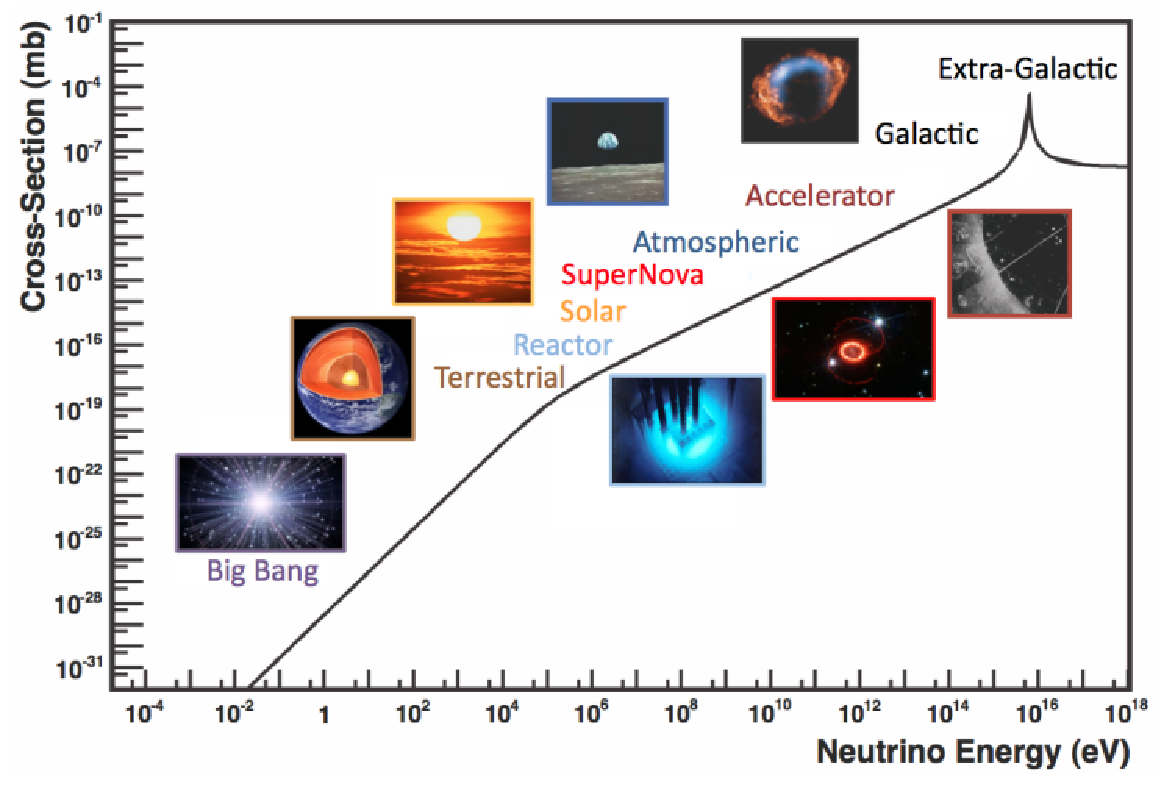
\includegraphics[width=\textwidth, trim={0mm 0mm 0mm 0mm}, clip,page=1]{Figures/Theory/EnergySpectrum.pdf}
  \end{subfigure}
  \caption{The cross-section of neutrinos from various natural and man-made sources as a function of neutrino energy. Taken from \cite{Formaggio:2012cpf}}
  \label{fig:NeutrinoOscillationPhysics_EnergySpectrum}
\end{figure}

\subsection{Solar Neutrinos}
\label{subsec:NeutrinoOscillationPhysics_SolarNeutrinos}

Solar neutrinos are emitted from fusion reaction chains at the center of the Sun. The solar neutrino flux, given as a function of neutrino energy for different fusion and decay chains, is illustrated in \autoref{fig:NeutrinoOscillationPhysics_SolarNeutrinoFlux}. Whilst proton-proton fusion generates the largest flux of neutrinos, the neutrinos are of low energy and are difficult to reconstruct due to the IBD interaction threshold of \quickmath{1.8\text{MeV}}. Consequently, most experiments focus on the neutrinos from the decay of \quickmath{^{8}B} (via \quickmath{^{8}B \rightarrow ^{8}Be^{*} + e^{+} + \nu_{e}}), which are higher energy.

\begin{figure}[h]
  \begin{subfigure}[t]{0.80\textwidth}
    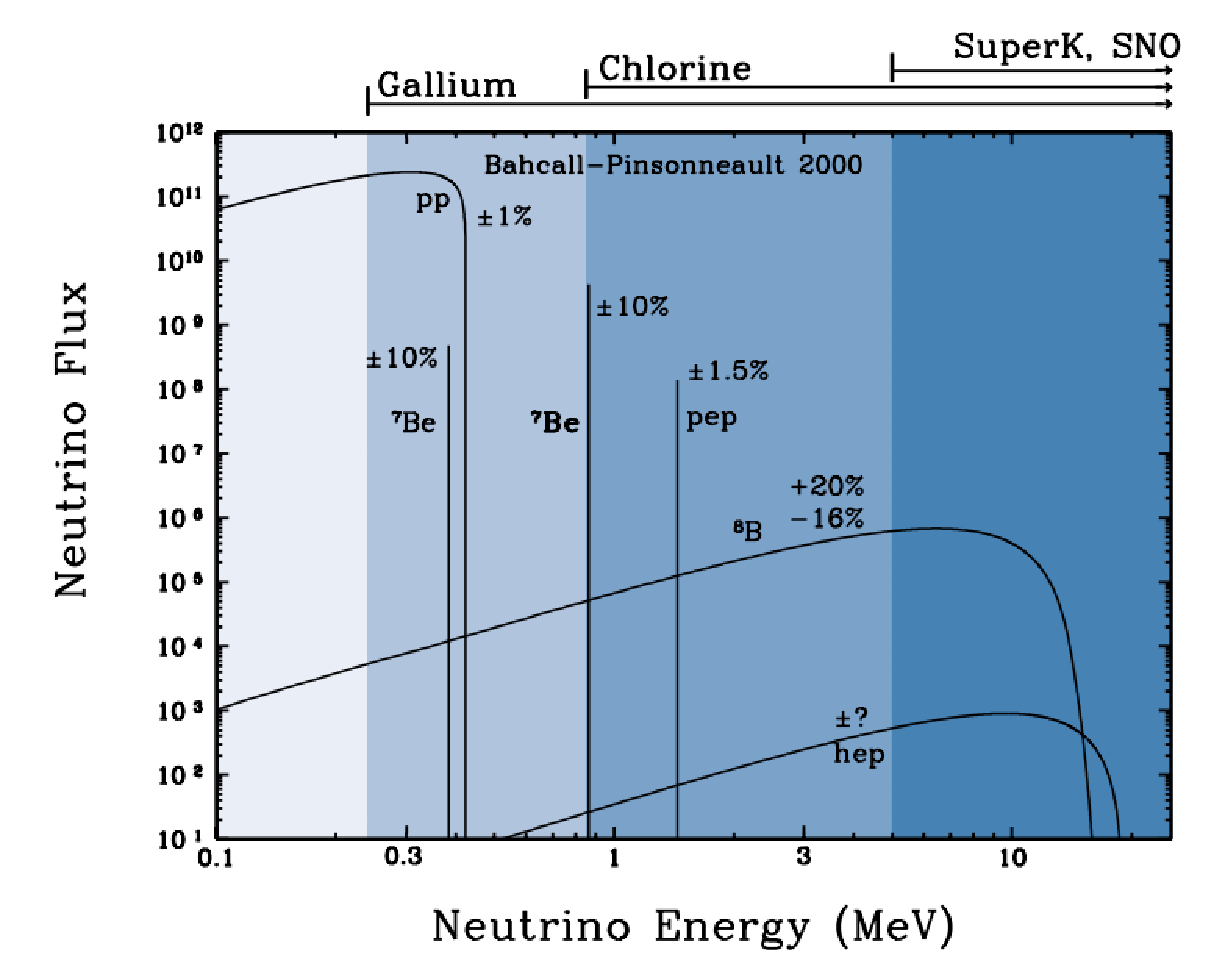
\includegraphics[width=\textwidth, trim={0mm 0mm 0mm 0mm}, clip,page=1]{Figures/Theory/SolarNeutrinoFlux.pdf}
  \end{subfigure}
  \caption{The solar neutrino flux as a function of neutrino energy for various fusion reactions and decay chains as predicted by the Standard Solar Model. Taken from \cite{Bellerive2004-ur}.}
  \label{fig:NeutrinoOscillationPhysics_SolarNeutrinoFlux}
\end{figure}

The first measurements of solar neutrinos observed a significant reduction in the event rate compared to predictions from the Standard Solar Model \cite{PhysRevLett.20.1205, Vinyoles2017-vv}. The proposed solution to this ``solar neutrino problem'' was \quickmath{\nu_{e} \leftrightarrow \nu_{\mu}} oscillations in a precursory version of the PMNS model \cite{Gribov1969-xi}. The Kamiokande \cite{PhysRevLett.63.16}, Gallex \cite{Hampel1999-of} and Sage \cite{PhysRevC.60.055801} experiments confirmed the \quickmath{\sim 0.5} factor deficit of solar neutrinos.

The conclusive solution to this problem was determined by the SNO collaboration \cite{Ahmad2002-zv}. Using a deuterium water target to observe \quickmath{^{8}B} neutrinos, the event rate of charged current (CC), neutral current (NC), and elastic scattering (ES) interactions (Given in \autoref{eq:NeutrinoOscillationPhysics_SNOInteractions}) was simultaneously measured. CC events can only occur for electron neutrinos, whereas the NC channel is agnostic to neutrino flavour, and the ES reaction has a slight excess sensitivity to electron neutrino interactions. This meant that there were direct measurements of the \quickmath{\nu_{e}} and \quickmath{\nu_x} neutrino flux. It was concluded that the CC and ES interaction rates were consistent with the deficit previously observed. Most importantly, the NC reaction rate was only consistent with the others under the hypothesis of flavour transformation.

\begin{equation}
  \label{eq:NeutrinoOscillationPhysics_SNOInteractions}
  \begin{split}
    \nu_{e} + d &\rightarrow p + p + e^{-} \hspace{2cm} (CC) \\
    \nu_{x} + d &\rightarrow p + n + \nu_{x} \hspace{2.02cm} (NC) \\
    \nu_{x} + e^{-} &\rightarrow \nu_{x} + e^{-} \hspace{2.55cm} (ES)
  \end{split}
\end{equation}

Many experiments have since measured the neutrino flux of different interaction chains within the sun \cite{Borexino_Collaboration2018-of, Aharmim2006-yb, Agostini2020-so}. The most recent measurement was that of CNO neutrinos which were recently observed with \quickmath{5\sigma} significance by the Borexino collaboration. Future neutrino experiments aim to further these spectroscopic measurements of different fusion chains within the Sun \cite{Andringa2016-zd, Beacom2017-ff, An2016-gm}. Solar neutrinos act as an irreducible background for dark matter experiments like DARWIN but oscillation parameter measurements can be made \cite{aalbers2020solar}.

\subsection{Atmospheric Neutrinos}
\label{subsec:NeutrinoOscillationPhysics_AtmosphericNeutrinos}

The interactions of primary cosmic ray protons in Earth's upper atmosphere generate showers of energetic hadrons. These are mostly pions and kaons which when they decay produce a natural source of neutrinos spanning energies of MeV to TeV \cite{Gaisser2002-gl}. The main decay is via

\begin{equation}
  \label{eq:NeutrinoOscillationPhysics_PionDecay}
  \begin{split}
    \pi^{\pm} &\rightarrow \mu^{\pm} + (\nu_{\mu},\bar{\nu}_\mu) \\
    \mu^{\pm} &\rightarrow e^{\pm} + (\nu_{\mu},\bar{\nu}_\mu) + (\nu_{e},\bar{\nu}_e)
  \end{split}
\end{equation}

such that for a single pion decay, three neutrinos are typically produced. The atmospheric neutrino flux energy spectra as predicted by the Bartol \cite{Barr_2004}, Honda \cite{Honda_2007, PhysRevD.70.043008, Honda:2011}, and FLUKA \cite{etde_20239111} models are illustrated in \autoref{fig:NeutrinoOscillationPhysics_AtmosphericNeutrinoFlux}. The flux distribution peaks at an energy of \quickmath{O(10) \text{GeV}}. The uncertainties associated with these models are dominated by the hadronic production of kaon and pions as well as the primary cosmic flux. 

\begin{figure}[h]
  \begin{subfigure}[t]{0.80\textwidth}
    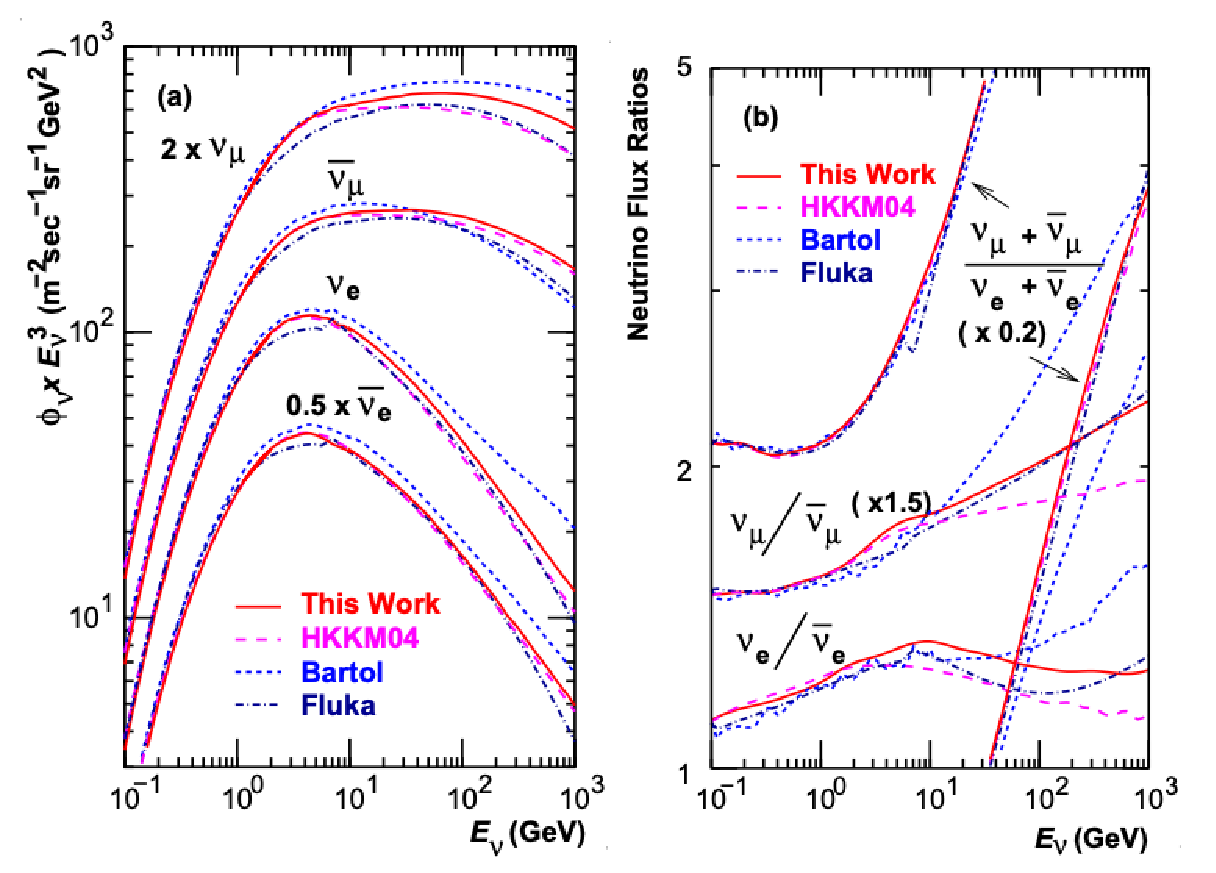
\includegraphics[width=\textwidth, trim={0mm 0mm 0mm 0mm}, clip,page=1]{Figures/Theory/AtmosphericNuFlux.pdf}
  \end{subfigure}
  \caption{Left panel: The atmospheric neutrino flux for different neutrino flavours as a function of neutrino energy as predicted by the 2007 Honda model (``This work'') \cite{Honda_2007}, the 2004 Honda model (``HKKM04'')\cite{PhysRevD.70.043008}, the Bartol model \cite{Barr_2004} and the FLUKA model \cite{etde_20239111}. Right panel: The ratio of the muon to electron neutrino flux as predicted by all the quoted models. Both figures taken from \cite{Honda_2007}.}
  \label{fig:NeutrinoOscillationPhysics_AtmosphericNeutrinoFlux}
\end{figure}

Unlike long-baseline experiments which have a fixed baseline, the distance atmospheric neutrinos propagate is dependent upon the zenith angle at which they interact. This is illustrated in \autoref{fig:NeutrinoOscillationPhysics_ZenithAngle}. Neutrinos that are generated directly above the detector (\quickmath{\cos(\theta)=1.0}) have a baseline equivalent to the height of the atmosphere whereas neutrinos that interact directly below the detector (\quickmath{\cos(\theta)=-1.0}) have to travel a length equal to the diameter of the  Earth. This means atmospheric neutrinos have a baseline that varies from \quickmath{O(20)\text{km}} to \quickmath{O(6 \times 10^{3})\text{km}}. Any neutrino generated at or below the horizon will be subject to matter effects as they propagate through the Earth.

\begin{figure}[h]
  \begin{subfigure}[t]{0.40\textwidth}
    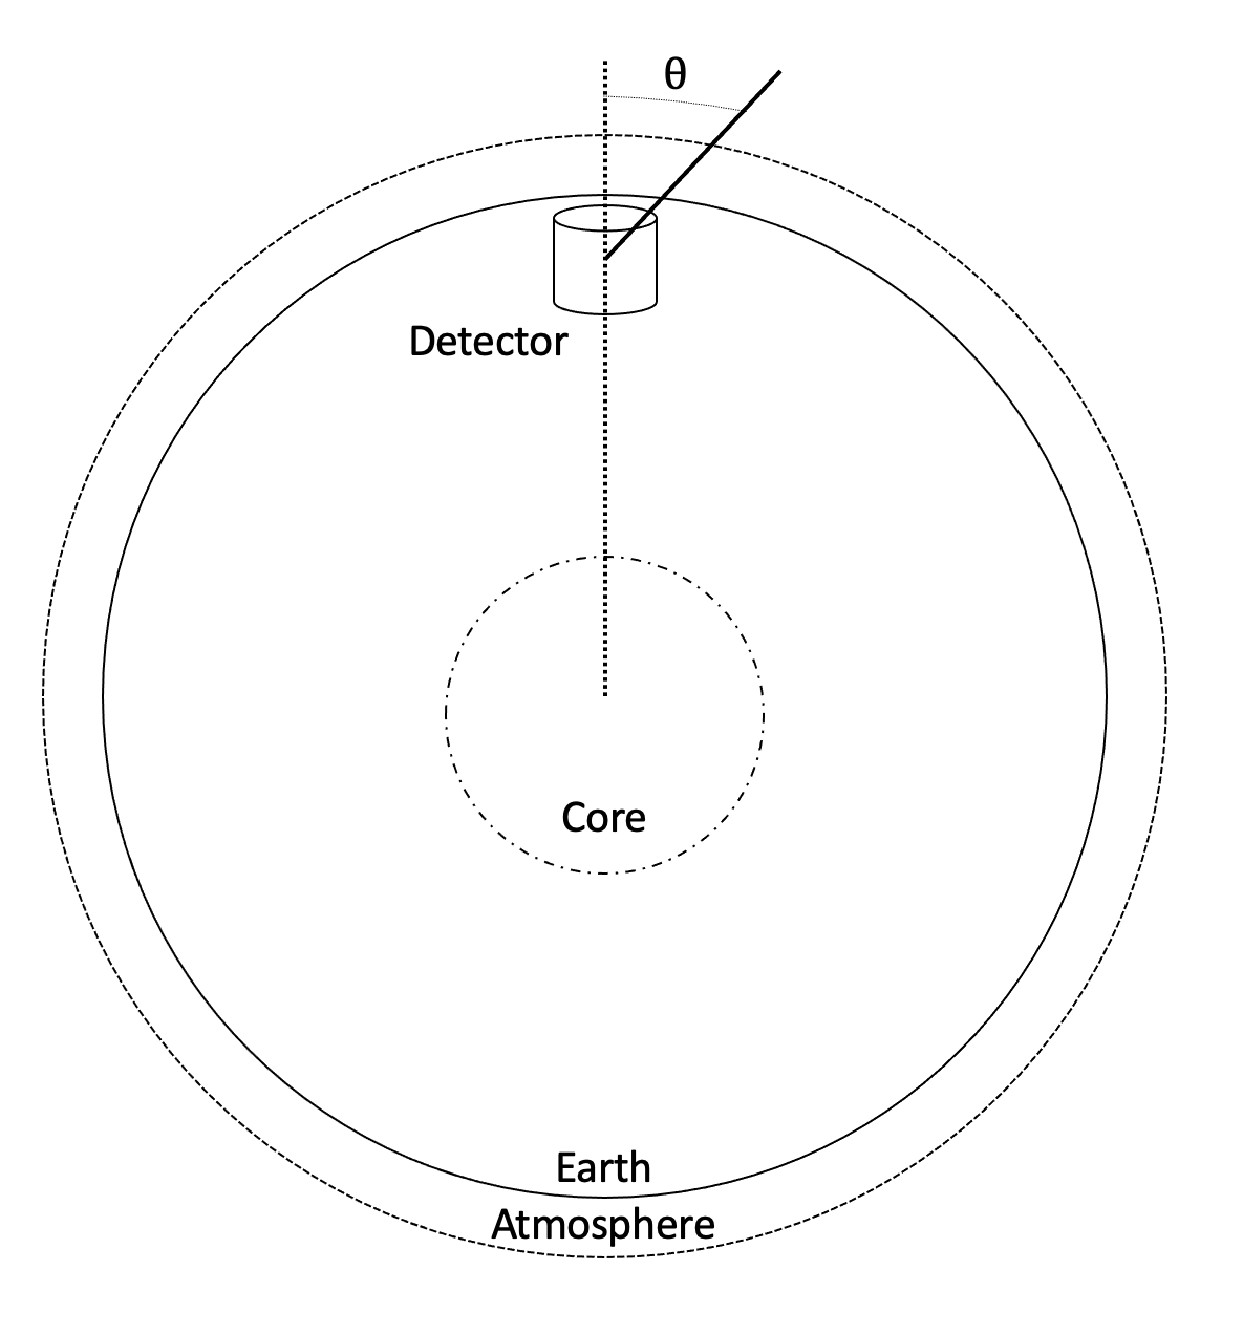
\includegraphics[width=\textwidth, trim={0mm 0mm 0mm 0mm}, clip,page=1]{Figures/Theory/ZenithAngle.pdf}
  \end{subfigure}
  \caption{A diagram illustrating the definition of zenith angle as used in the Super Kamiokande experiment \cite{Ashie_2005}.}
  \label{fig:NeutrinoOscillationPhysics_ZenithAngle}
\end{figure}

\autoref{fig:NeutrinoOscillationPhysics_NuFluxZenithAngleDep} highlights the neutrino flux as a function of the zenith angle for different slices of neutrino energy. For medium to high-energy neutrinos (and to a lesser degree for low-energy neutrinos), the flux is approximately symmetric around \quickmath{\cos(\theta)=0}. To the accuracy of this approximation, the systematic uncertainties associated with atmospheric flux for comparing upward-going and down-going neutrino cancels. This allows the down-going events, which are mostly insensitive to oscillation probabilities, to act as an unoscillated prediction (similar to a near detector in an accelerator neutrino experiment).

\begin{figure}[h]
  \begin{subfigure}[t]{0.90\textwidth}
    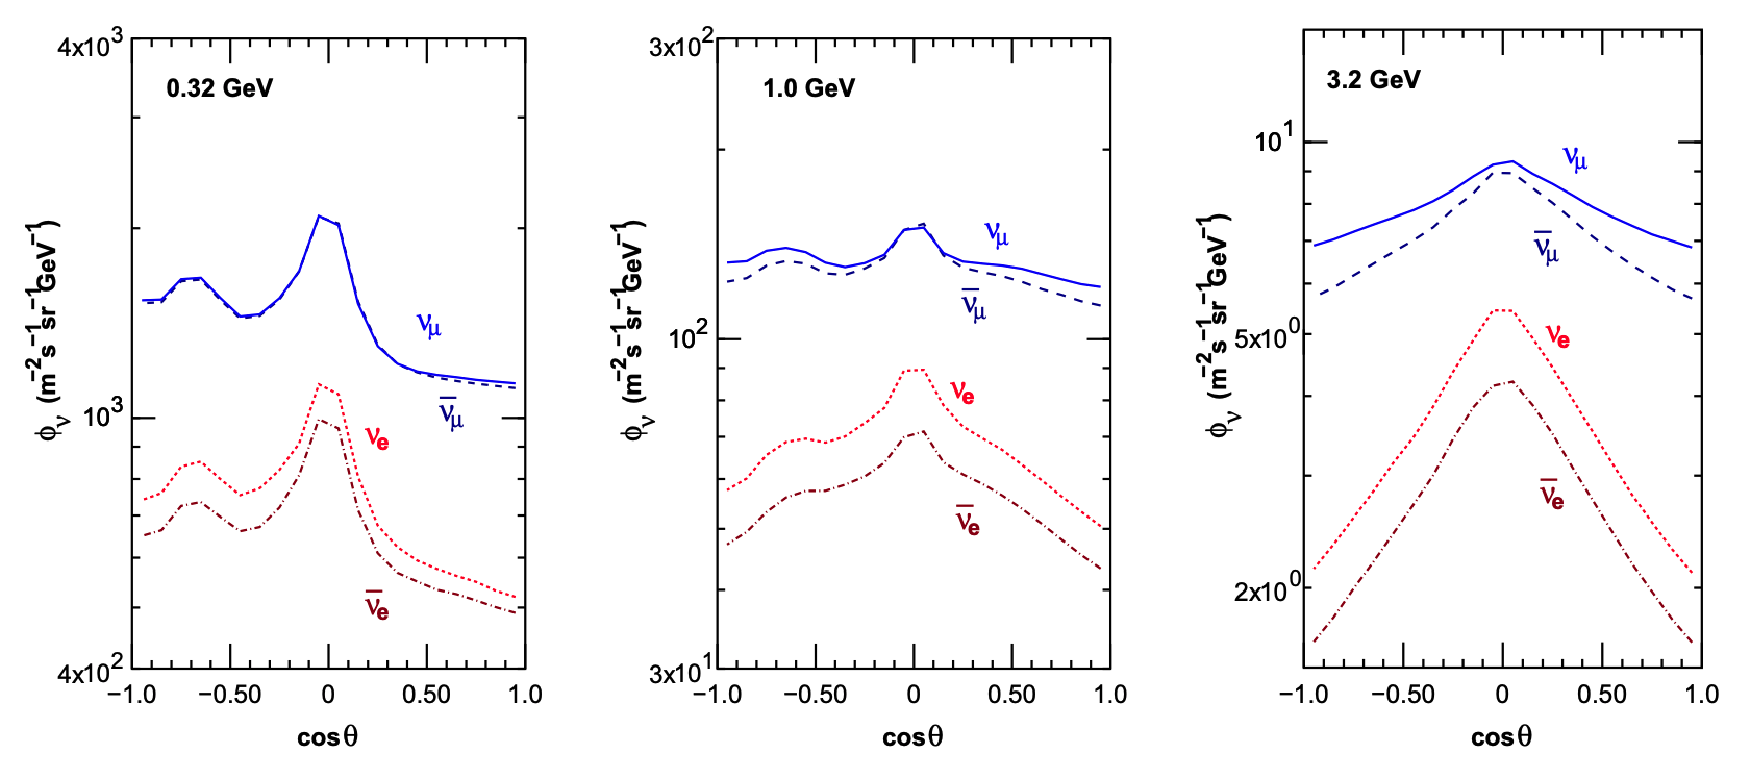
\includegraphics[width=\textwidth, trim={0mm 0mm 0mm 0mm}, clip,page=1]{Figures/Theory/NuFluxZenithAngleDep.pdf}
  \end{subfigure}
  \caption{Prediction of \quickmath{\nu_e, \bar{\nu}_{e}, \nu_{\mu}, \bar{\nu}_{\mu}} fluxes as a function of zenith angle as calculated by the HKKM model \cite{Honda:2011}. The left, middle and right panels represent three values of neutrino energy, \quickmath{0.32\text{GeV}}, \quickmath{1.0\text{GeV}} and \quickmath{3.2\text{GeV}} respectively. Predictions for other models including Bartol \cite{Barr_2004}, Honda \cite{Honda_2007} and FLUKA \cite{etde_20239111} are given in \cite{Ashie_2005}.}
  \label{fig:NeutrinoOscillationPhysics_NuFluxZenithAngleDep}
\end{figure}

Precursory hints of atmospheric neutrinos were observed in the mid-1960s searching for \quickmath{\overset{(-)}{\nu_\mu} + X \rightarrow X^{*} + \mu^{\pm}} \cite{Reines1965-cf}, although it was called an anomaly at the time of measurement. This was succeeded with the IMB-3 \cite{PhysRevLett.66.2561} and Kamiokande \cite{Hirata1992-qz} experiments which measured the ratio of muon neutrinos compared to electron neutrinos \quickmath{R(\nu_{\mu}/\nu_{e})}. Both experiments were found to have a consistent deficit of muon neutrinos, with \quickmath{R(\nu_{\mu}/\nu_{e}) = 0.67 \pm 0.17} and \quickmath{R(\nu_{\mu}/\nu_{e}) = 0.60 \substack{+ 0.07 \\ -0.06} \pm 0.05}. %Soudan-2 \cite{Allison1997-qz} determined similar measurements.
Super-Kamiokande (SK) \cite{Ashie_2005} extended this analysis by fitting oscillation parameters in \quickmath{P(\nu_\mu \rightarrow \nu_\tau)} which found best fit parameters \quickmath{\sin^{2}(2\theta) > 0.92} and \quickmath{1.5 \times 10^{-3} < \Delta m^{2} < 3.4 \times 10^{-3} \text{eV}^{2}}.

Since then, atmospheric neutrino experiments have been making precision measurements of the \sinsqatm and \quickmath{\Delta m^{2}_{32}} oscillation parameters.
%, and to a lesser extent the sign of \delmsqatm through the matter resonance present for any neutrinos passing through the Earth.
Atmospheric neutrino oscillation is dominated by \quickmath{P(\nu_{\mu} \rightarrow \nu_{\tau})}, where SK observed a \quickmath{4.6\sigma} discovery of \quickmath{\nu_{\tau}} appearance \cite{Li_2018}. \autoref{fig:NeutrinoOscillationPhysics_AtmosphericParamContour} illustrates the current estimates on the atmospheric mixing parameters from a wide range of atmospheric and accelerator neutrino observatories.

\begin{figure}[h]
  \begin{subfigure}[t]{0.90\textwidth}
    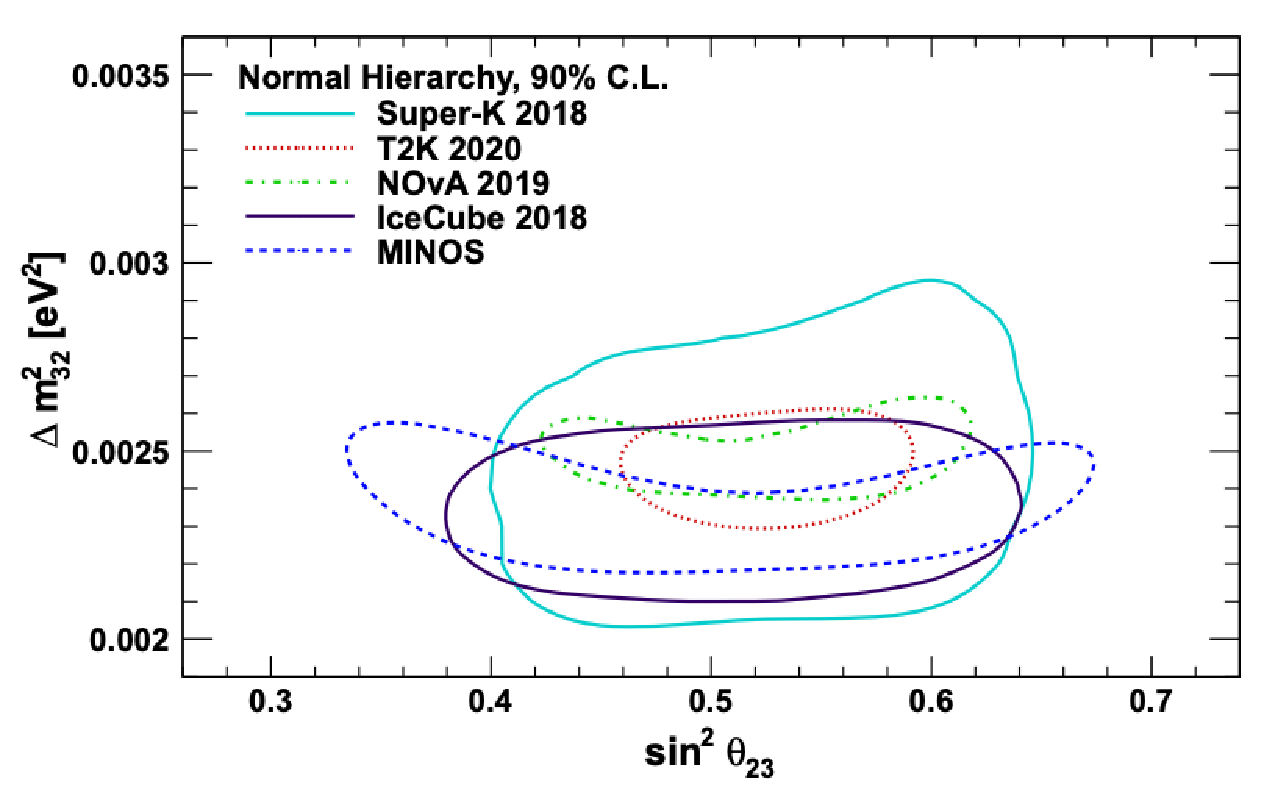
\includegraphics[width=\textwidth, trim={0mm 0mm 0mm 0mm}, clip,page=1]{Figures/Theory/AtmosphericParams.pdf}
  \end{subfigure}
  \caption{Constraints on the atmospheric oscillation parameters, \sinsqatm and \delmsqatm, from atmospheric and long baseline experiments: SK \cite{Kamiokande_Collaboration2017-nf}, T2K \cite{T2K_Collaboration2018-sm}, \quickmath{\text{NO}\nu\text{A}} \cite{Acero2019-rw}, IceCube \cite{Aartsen2018-cz} and MINOS \cite{Adamson2014-tt}. Figure taken from \cite{Athar_2022}.}
  \label{fig:NeutrinoOscillationPhysics_AtmosphericParamContour}
\end{figure}

\subsection{Accelerator Neutrinos}
\label{subsec:NeutrinoOscillationPhysics_AcceleratorNeutrinos}

The concept of using a man-made ``neutrino beam'' was first realised in 1962 \cite{Danby1962-ph}.
%and led to the first discovery that \quickmath{\nu_{e}} and \quickmath{\nu_{\mu}} were in fact different particles.
Since then, many experiments have followed which all use the same fundamental concepts. Typically, a proton beam is aimed at a target producing charged mesons that decay to neutrinos. The mesons can be sign-selected by the use of magnetic focusing horns to generate a neutrino or antineutrino beam.
%Absorbing material and the rock between the target and detector absorb all particles barring the neutrinos.
Pions are the primary meson that decay and depending on the orientation of the magnetic field, a muon (anti-)neutrino beam is generated via \quickmath{\pi^{+} \rightarrow \mu^{+} + \nu_{\mu}} or \quickmath{\pi^{-} \rightarrow \mu^{-} + \bar{\nu}_{\mu}}. The decay of muons and kaons does result in an irreducible intrinsic electron neutrino background. In T2K, this background contamination is \quickmath{O(<1\%)} \cite{Abe_2013}. There is also an approximately \quickmath{\sim 5\%} ``wrong-sign'' neutrino background of \quickmath{\bar{\nu}_{\mu}} generated via the same decays. As the beam is generated by proton interactions (rather than anti-proton interactions), the wrong-sign component in the antineutrino beam is larger when operating in neutrino mode.

Tuning the proton energy in the beam and using beam focusing techniques allows the neutrino energy to be set to a value that maximises the disappearance oscillation probability in the \quickmath{L/E} term in \autoref{eq:NeutrinoOscillationPhysics_PMNS_2FlavourOscProb}.
%As the inital proton beam can be tuned resulting in a tunable neutrino energy spectra, the advantage of these type of experiments is that they can be focused in on the oscillation dip presented by the \quickmath{L/E} term in \autoref{eq:NeutrinoOscillationPhysics_PMNS_2FlavourOscProb} using the two flavour approximation.
This means that accelerator experiments are typically more sensitive to the mixing parameters as compared to a natural neutrino source. However, the disadvantage compared to atmospheric neutrino experiments is that the baseline has to be shorter due to the lower flux. Consequently, there is typically less sensitivity to matter effects and the ordering of the neutrino mass eigenstates.

A neutrino experiment measures

\begin{equation}
  \label{eq:NeutrinoOscillationPhysics_DetectorMeasurement}
  R(\vec{x}) = \Phi(E_{\nu}) \times \sigma(E_{\nu}) \times \epsilon(\vec{x}) \times P(\nu_{\alpha} \rightarrow \nu_{\beta}),
\end{equation}

where \quickmath{R(\vec{x})} is the event rate of neutrinos at position \quickmath{\vec{x}}, \quickmath{\Phi(E_{\nu})} is the flux of neutrinos with energy \quickmath{E_{\nu}}, \quickmath{\sigma(E_{\nu})} is the cross-section of the neutrino interaction and \quickmath{\epsilon(\vec{x})} is the efficiency and resolution of the detector. In order to leverage the most out of an accelerator neutrino experiment, the flux and cross-section systematics need to be constrained. This is typically done via the use of a ``near detector'', situated at a baseline of \quickmath{O(1)\text{km}}. This detector observes the unoscillated neutrino flux and constrains the parameters used within the flux and cross-section model.

The first accelerator experiments to precisely measure oscillation parameters were MINOS \cite{PhysRevLett.97.191801} and K2K \cite{PhysRevLett.9.36}.
These experiments confirmed the \quickmath{\nu_{\mu}} disappearance seen in atmospheric neutrino experiments by finding consistent parameter values for \sinsqatm and \delmsqatm.
The current generation of accelerator neutrino experiments, T2K and \NOVA extended this field by observing \quickmath{\bar{\nu}_{\mu} \rightarrow \bar{\nu}_{e}} and lead the sensitivity to atmospheric mixing parameters as seen in \autoref{fig:NeutrinoOscillationPhysics_AtmosphericParamContour} \cite{PhysRevLett.123.151803}.
The two experiments differ in their peak neutrino energy, baseline, and detection technique.
The \NOVA experiment is situated at a baseline of \quickmath{810\text{km}} from the NuMI beamline which delivers \quickmath{2\text{GeV}} neutrinos.
The T2K neutrino beam is peaked around \quickmath{0.6 \text{GeV}} and propagates \quickmath{295\text{km}}.
The \NOVA experiment also uses functionally identical detectors (near and far) which allow the approximate cancellation of detector systematics whereas T2K uses a plastic scintillator technique at the near detector and a water Cherenkov far detector.
The future generation experiments DUNE \cite{Abi2020-cm} and Hyper-Kamiokande \cite{Hyper-Kamiokande_Proto-Collaboration2015-ac} will succeed these experiments as the high-precision era of neutrino oscillation parameter measurements develops.

Several anomalous results have been observed in the LSND \cite{PhysRevD.64.112007} and MiniBooNE \cite{PhysRevLett.110.161801} detectors which were designed with purposefully short baselines. Parts of the neutrino community attributed these results to oscillations induced by a fourth ``sterile'' neutrino \cite{Blanco_2020} but several searches in other experiments, MicroBooNE \cite{10.48550/arxiv.2110.14054} and KARMEN \cite{PhysRevD.65.112001}, found no hints of additional neutrino species. The solution to the anomalous results is still being determined.

\subsection{Reactor Neutrinos}
\label{subsec:NeutrinoOscillationPhysics_ReactorNeutrinos}

As illustrated in the first discovery of neutrinos (\autoref{sec:NeutrinoOscillationPhysics_Discovery}), nuclear reactors are a very useful man-made source of electron antineutrinos. For reactors that use low-enriched uranium \quickmath{^{235}\text{U}} as fuel, the antineutrino flux is dominated by the \quickmath{\beta}-decay fission of \quickmath{^{235}\text{U}}, \quickmath{^{238}\text{U}}, \quickmath{^{239}\text{Pu}} and \quickmath{^{241}\text{Pu}} \cite{Kim2013-ye} as illustrated in \autoref{fig:NeutrinoOscillationPhysics_ReactorNeutrinoProduction}.

\begin{figure}[h]
  \begin{subfigure}[t]{0.90\textwidth}
    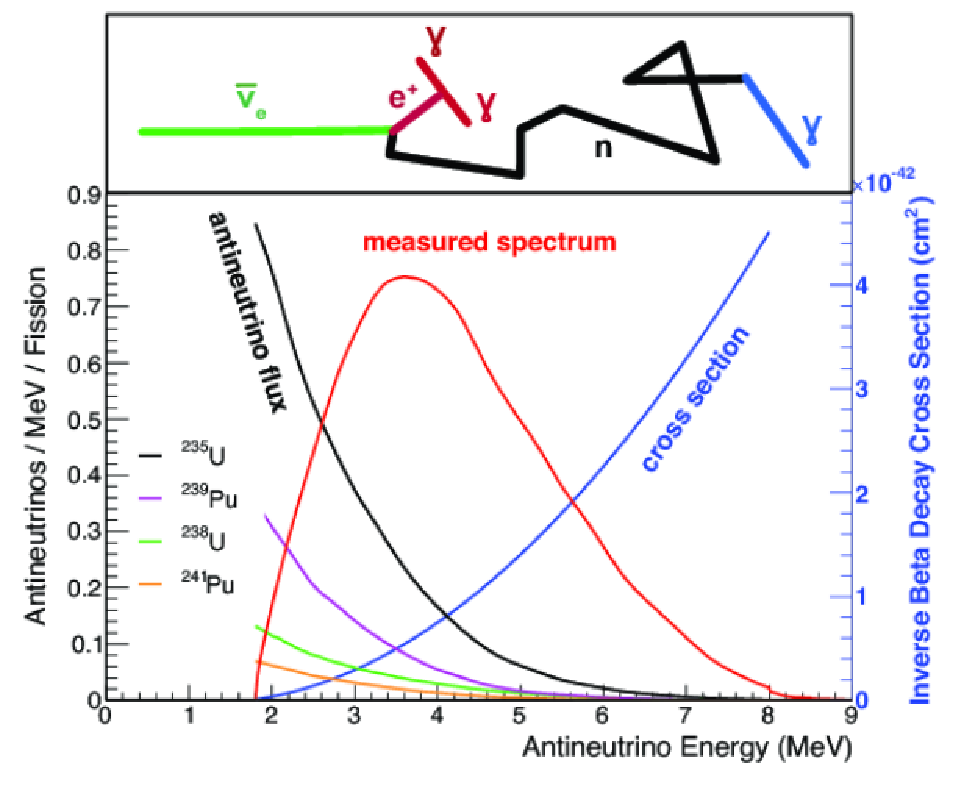
\includegraphics[width=\textwidth, trim={0mm 0mm 0mm 0mm}, clip,page=1]{Figures/Theory/ReactorNeutrinoProduction.pdf}
  \end{subfigure}
  \caption{Reactor electron antineutrino fluxes for \quickmath{^{235}\text{U}} (Black), \quickmath{^{238}\text{U}} (Green), \quickmath{^{239}\text{Pu}} (Purple), and \quickmath{^{241}\text{Pu}} (Orange) isotopes. The inverse \quickmath{\beta}-decay cross-section (Blue) and corresponding measurable neutrino spectrum (Red) are also given. Top panel: Schematic of Inverse \quickmath{\beta}-decay interaction including the eventual capture of the emitted neutron. This capture emits a \quickmath{\gamma}-ray which provides a second signal of the event. Taken from \cite{SajjadAthar:2021prg}.}
  \label{fig:NeutrinoOscillationPhysics_ReactorNeutrinoProduction}
\end{figure}

Due to their low energy, reactor electron antineutrinos predominantly interact via the inverse \quickmath{\beta}-decay (IBD) interaction. The typical signature contains two signals delayed by \quickmath{O(200)\mu\text{s}}; firstly the prompt photons from positron annihilation, and secondly the photons emitted (\quickmath{E_{tot}^{\gamma} = 2.2\text{MeV}}) from de-excitation after neutron capture on hydrogen. Searching for both signals improves the detector's ability to distinguish between background and signal events \cite{Abe2022-ij}. Recently, SK included gadolinium dopants into the ultra-pure water to increase the energy released from the photon cascade to \quickmath{\sim 8\text{MeV}} and reduce the time of the delayed signal to \quickmath{\sim 28 \mu \text{s}}.

There are many short baseline experiments (\quickmath{\text{L} \sim O(1)\text{km}}) that have measured the \sinsqreac and \delmsqatm oscillation parameters. Daya Bay \cite{PhysRevLett.108.171803}, RENO \cite{PhysRevLett.108.191802} and Double Chooz \cite{PhysRevLett.108.131801} have all provided precise measurements, with the first discovery of a non-zero \quickmath{\theta_{13}} made by Daya Bay and RENO (and complemented by T2K \cite{PhysRevLett.108.131801}). The constraints on \sinsqreac by the reactor experiments lead the field and are often used as external inputs to accelerator neutrino experiments to improve their sensitivity to \dcp and mass hierarchy determination.
%One curiosity of these short baseline reactor experiments is the `\quickmath{5 \text{MeV}} excess' \cite{Berryman_2019}. First observed in 2014 \cite{For_the_RENO_Collaboration2015-zy, Abe_2014}, all three experiments listed observed a shape excess in events around \quickmath{E_{\nu} \sim 5 \text{MeV}}. The reason behind this excess is speculated to be either oscillations to sterile neutrinos or a fault in the Huber-Mueller model \cite{Mueller_2011}. At this time, the latter is favoured as Daya Bay \cite{PhysRevLett.123.111801} observed substantial evidence (\quickmath{4.0\sigma}) of correlation between the excess and the \quickmath{^{235}\text{U}} electron antineutrino flux.
%Other neutrino experiments, PROSPECT \cite{PhysRevD.103.032001} and STEREO \cite{STEREO} show similar results data to help determine the cause of the excess.
JUNO-TAO \cite{junocollaboration2020tao}, a small collaboration within the larger JUNO experiment, is a next-generation reactor experiment that aims to precisely measure the isotopic antineutrino yields from the different fission chains. Alongside this, it aims to explain the `\quickmath{5 \text{MeV}} excess' \cite{For_the_RENO_Collaboration2015-zy, Abe_2014, PhysRevLett.123.111801} by conducting a search for sterile neutrinos with a mass scale of around \quickmath{1 \text{eV}}.

Kamland \cite{Decowski2016-hh} is the only experiment to have observed reactor neutrinos using a long baseline (flux weighted averaged baseline of \quickmath{L \sim 180\text{km}}) which allows it to have sensitivity to \delmsqsol. Combined with the SK solar neutrino experiment, the combined analysis puts the most stringent constraint on \delmsqsol \cite{PhysRevD.83.052002}.

\section{Summary}
\label{sec:Theory_Summary}

Since observing the first evidence of neutrino oscillations in the late 1990's, numerous measurements of the mixing parameters have been made. Many experiments use neutrinos as a tool for discovery of new physics (diffuse supernoave background, neutrinoless double beta decay and others) so the PMNS parameters are summarised in the Particle Data Group (PDG) review tables. The analysis presented in this thesis focuses on the 2020 T2K oscillation analysis presented in \cite{Dunne2020-uf} where the 2018 PDG constraints \cite{Tanabashi2018-hp} were used. These constraints are outlined in \autoref{tab:Theory_PDGConstraints}.

\begin{table}[ht!]
    \centering
    \begin{tabular}{c|c}
      \hline
      Parameter & 2018 Constraint \\
      \hline
      \quickmath{\sin^{2}(\theta_{12})} & \quickmath{0.307 \pm 0.013} \\
      \quickmath{\Delta m^{2}_{21}} & \quickmath{(7.53 \pm 0.18) \times 10^{-5} \text{eV}^{2}} \\
      \quickmath{\sin^{2}(\theta_{13})} & \quickmath{(2.12 \pm 0.08) \times 10^{-2}} \\
      \quickmath{\sin^{2}(\theta_{23})} (I.H., Q1) & \quickmath{0.421^{+0.033}_{-0.025}} \\
      \quickmath{\sin^{2}(\theta_{23})} (I.H., Q2) & \quickmath{0.592^{+0.023}_{-0.030}} \\
      \quickmath{\sin^{2}(\theta_{23})} (N.H., Q1) & \quickmath{0.417^{+0.025}_{-0.028}} \\
      \quickmath{\sin^{2}(\theta_{23})} (N.H., Q2) & \quickmath{0.597^{+0.024}_{-0.030}} \\
      \quickmath{\Delta m^{2}_{32}} (I.H.) & \quickmath{(-2.56 \pm 0.04) \times 10^{-3} \text{eV}^{2}} \\
      \quickmath{\Delta m^{2}_{32}} (N.H.) & \quickmath{(2.51 \pm 0.05) \times 10^{-3} \text{eV}^{2}} \\
      \hline
      \hline
    \end{tabular}
    \caption{The 2018 Particle Data Group constraints of the oscillation parameters taken from \cite{Tanabashi2018-hp}. The value of \delmsqatm is given for both normal hierarchy (N.H.) and inverted hierarchy (I.H.) and \sinsqatm is broken down by whether its value is below (Q1) or above (Q2) \quickmath{0.5}.}
    \label{tab:Theory_PDGConstraints}
\end{table}

The \sinsqreac measurement stems from the electron antineutrino disappearance, \quickmath{P(\bar{\nu}_{e} \rightarrow \bar{\nu}_{e})}, and is take as the  average best-fit from the combination of Daya Bay, Reno and Double Chooz. It is often used as a prior uncertainty within other neutrino oscillation experiments, typically termed the reactor constraint. The \sinsqsol parameter is predominantely measured through electron neutrino disappearance, \quickmath{P(\nu_{e} \rightarrow \nu_{\mu,\tau})}, in solar neutrino experiments. The long-baseline reactor neutrino experiment Kamland also has sensitivity to this parameter and is used in a joint fit to solar data from SNO and SK, using the reactor constraint. Measurements of \sinsqatm are made by long-baseline and atmospheric neutrino experiments. The PDG value is a joint fit of T2K, \NOVA, MINOS and IceCube DeepCore experiments. The latest T2K-only meaurement, provided at Neutrino2020 and is the basis of this thesis, is given as \quickmath{\sin^{2}(\theta_{23}) = 0.546^{+0.024}_{-0.046}} \cite{Dunne2020-uf}. The PDG constraint on \delmsqsol is provided by the KamLAND experiment using solar and geoneutrino data. This measurement utilised a \sinsqreac constraint from accelerator (T2K, MINOS) and reactor neutrino (Daya Bay, RENO, Double Chooz) experiments. Accelerator measurements make some of the most stringent constraints on \delmsqatm although atmospheric experiments have more sensitivity to the mass hierarchy determination. The PDG performs a joint fit of accelerator and atmospheric data, in both normal and inverted hierarchy separately. The latest T2K-only result is \quickmath{\Delta m^{2}_{32} = 2.49^{+0.058}_{-0.082} \times 10^{-3}\text{eV}^{2}} favouring normal hierarchy \cite{Dunne2020-uf}. The value of \dcp is largely undetermined. CP-conserving values of \quickmath{0} and \quickmath{\pi} were rejected with \quickmath{\sim 2\sigma} intervals, as published in Nature, although more recent analysis have reduced the rejection intervals to \quickmath{90\%}. Since the 2018 PDG publication, there has been a new measurement of \quickmath{\sin^{2}(\theta_{13}) = (2.20 \pm 0.07) \times 10^{-2}} \cite{Workman:2022ynf}, alongside updated \delmsqatm and \sinsqatm measurements.

Throughout this thesis, several sample spectra predictions and contours are presented which require oscillation parameters to be assumed. \autoref{tab:Theory_ParameterSets} defines two sets of oscillation parameters, with ``Asimov A'' set being close to the preferred values from a previous T2K-only fit \cite{PhysRevLett.112.181801} and ``Asimov B'' being CP-conserving and further from maximal \quickmath{\theta_{23}} mixing.

\begin{table}[ht!]
    \centering
    \begin{tabular}{c|c|c}
      \hline
      \hline
      Parameter & Asimov A & Asimov B \\
      \hline
      \quickmath{\Delta m^{2}_{12}} & \multicolumn{2}{c}{\quickmath{7.53 \times 10^{-5} \text{eV}^{2}}} \\ \hline
      \quickmath{\Delta m^{2}_{32}} & \multicolumn{2}{c}{\quickmath{2.509 \times 10^{-3} \text{eV}^{2}}} \\ \hline
      \quickmath{\sin^{2}\left(\theta_{12}\right)} & \multicolumn{2}{c}{\quickmath{0.304}} \\ \hline
      \quickmath{\sin^{2}\left(\theta_{13}\right)} & \multicolumn{2}{c}{\quickmath{0.0219}} \\ \hline
      \quickmath{\sin^{2}\left(\theta_{23}\right)} & \quickmath{0.528} & \quickmath{0.45} \\ \hline
      \quickmath{\delta_{CP}} & \quickmath{-1.601} & \quickmath{0.0} \\ \hline
      \hline
    \end{tabular}
    \caption{Reference values of the neutrino oscillation parameters for two different oscillation parameter sets.}
    \label{tab:Theory_ParameterSets}
\end{table}

  \chapter{T2K and SK Experiment Overview}
\label{chap:T2KSKExp}

As the successor of the Kamiokande experiment, the Super-Kamiokande (SK) collaboration has been leading atmospheric neutrino oscillation analyses for over two decades. The detector has provided some of the strongest constraints on proton decay and the first precise measurements of the \delmsqatm and \sinsqatm neutrino oscillation parameters.
%The ability of the detector to observe low-energy neutrino events has been significantly improved with the recent gadolinium doping of the ultra-pure water target.
The history, detection technique, and operation of the SK detector is described in \autoref{sec:T2KSKExp_SK}.

The Tokai-to-Kamioka (T2K) experiment was one of the first long-baseline experiments to use both neutrino and antineutrino beams to precisely measure the charge parity violation within the neutrino sector. The T2K experiment observed the first hints of a non-zero \sinsqreac measurement and continues to lead the field with the constraints it provides on \sinsqreac, \sinsqatm, \delmsqatm and \dcp.
In \autoref{sec:T2KSKExp_T2K}, the techniques that T2K use to generate the neutrino beam and constrain systematic parameter through near detector constraints are described.

%The techniques which T2K uses in generating its neutrino beam as well as the near-detector used to constrain the flux and cross-section parameters used in this analysis are documented in \autoref{sec:T2KSKExp_T2K}.

\section{The Super-Kamiokande Experiment}
\label{sec:T2KSKExp_SK}

The SK experiment began taking data in 1996 \cite{Fukuda1998-tw} and has had many modifications throughout its operation. There have been seven defined periods of data taking as noted in \autoref{tab:T2KSKExp_SKPeriods}. Data taking began in SK-I which ran for five years. Between the SK-I and SK-II periods, approximately \quickmath{55\%} of the PMTs were damaged during maintenance \cite{Abe_2014_SKCalib}. Those that survived were equally distributed throughout the detector in the SK-II era, which resulted in a reduced \quickmath{19\%} photo-coverage. From SK-III onwards, repairs to the detector meant the full suite of PMTs was operational recovering the \quickmath{40\%} photocoverage. Before the start of SK-IV, the data acquisition and electronic systems were upgraded. Between SK-IV and SK-V, a significant effort was placed into tank open maintenance and repair/replacement of defective PMTs, a task for which the author of this thesis was required. Consequently, the detector conditions were significantly different between the two operational periods. SK-VI marked the start of the SK-Gd era, with the detector being doped with gadolinium at a concentration of \quickmath{0.01\%}. SK-VII, which started during the writing of this thesis, has increased the gadolinium concentration to \quickmath{0.03\%} for continued operation \cite{10.5281/zenodo.6694761}.

The oscillation analysis presented within this thesis focuses on the SK-IV period of running and the data taking within it. This follows from the recent SK analysis presented in \cite{thesis_miao}. Therefore, the information presented within this section focuses on that period.

\begin{table}[ht!]
    \centering
    \begin{tabular}{c|l|l|c}
      \hline
      Period & Start Date & End Date & Live-time (days) \\
      \hline
      I & April 1996 & July 2001 & 1489.19 \\
      II & October 2002 & October 2005 & 798.59 \\
      III & July 2006 & September 2008 & 518.08 \\
      IV & September 2008 & May 2018 & 3244.4 \\
      V & January 2019 & July 2020 & 461.02 \\
      VI & July 2020 & May 2022 & 583.3 \\
      VII & May 2022 & Ongoing & N/A \\
      \hline 
      \hline
    \end{tabular}
    \caption{The various SK periods and respective live-time. The SK-VI live-time is calculated until \quickmath{1^{\text{st}}} April 2022. SK-VII started during the writing of this thesis.}
    \label{tab:T2KSKExp_SKPeriods}
\end{table}

\subsection{The SK Detector}
\label{subsec:T2KSKExp_SKDetector}

The basic structure of the Super-Kamiokande (SK) detector is a cylindrical tank with a diameter \quickmath{39.3\text{m}} and height \quickmath{41.1\text{m}} filled with ultrapure water \cite{Abe_2014_SKCalib}. A diagram of the significant components of the SK detector is given in \autoref{fig:T2KSKExp_SK_Diag}. The SK detector is situated in the Kamioka mine in Gifu, Japan. The mine is underground with roughly \quickmath{1\text{km}} rock overburden (\quickmath{2.7 \text{km}} water equivalent overburden) \cite{Fukuda2003-ly}. At this depth, the rate of cosmic ray muons is significantly decreased to a value of \quickmath{\sim 2\text{Hz}}. The top of the tank is covered with stainless steel which is designed as a working platform for maintenance, calibration, and location for high voltage and data acquisition electronics.

\begin{figure}[h]
  \begin{subfigure}[t]{0.95\textwidth}
    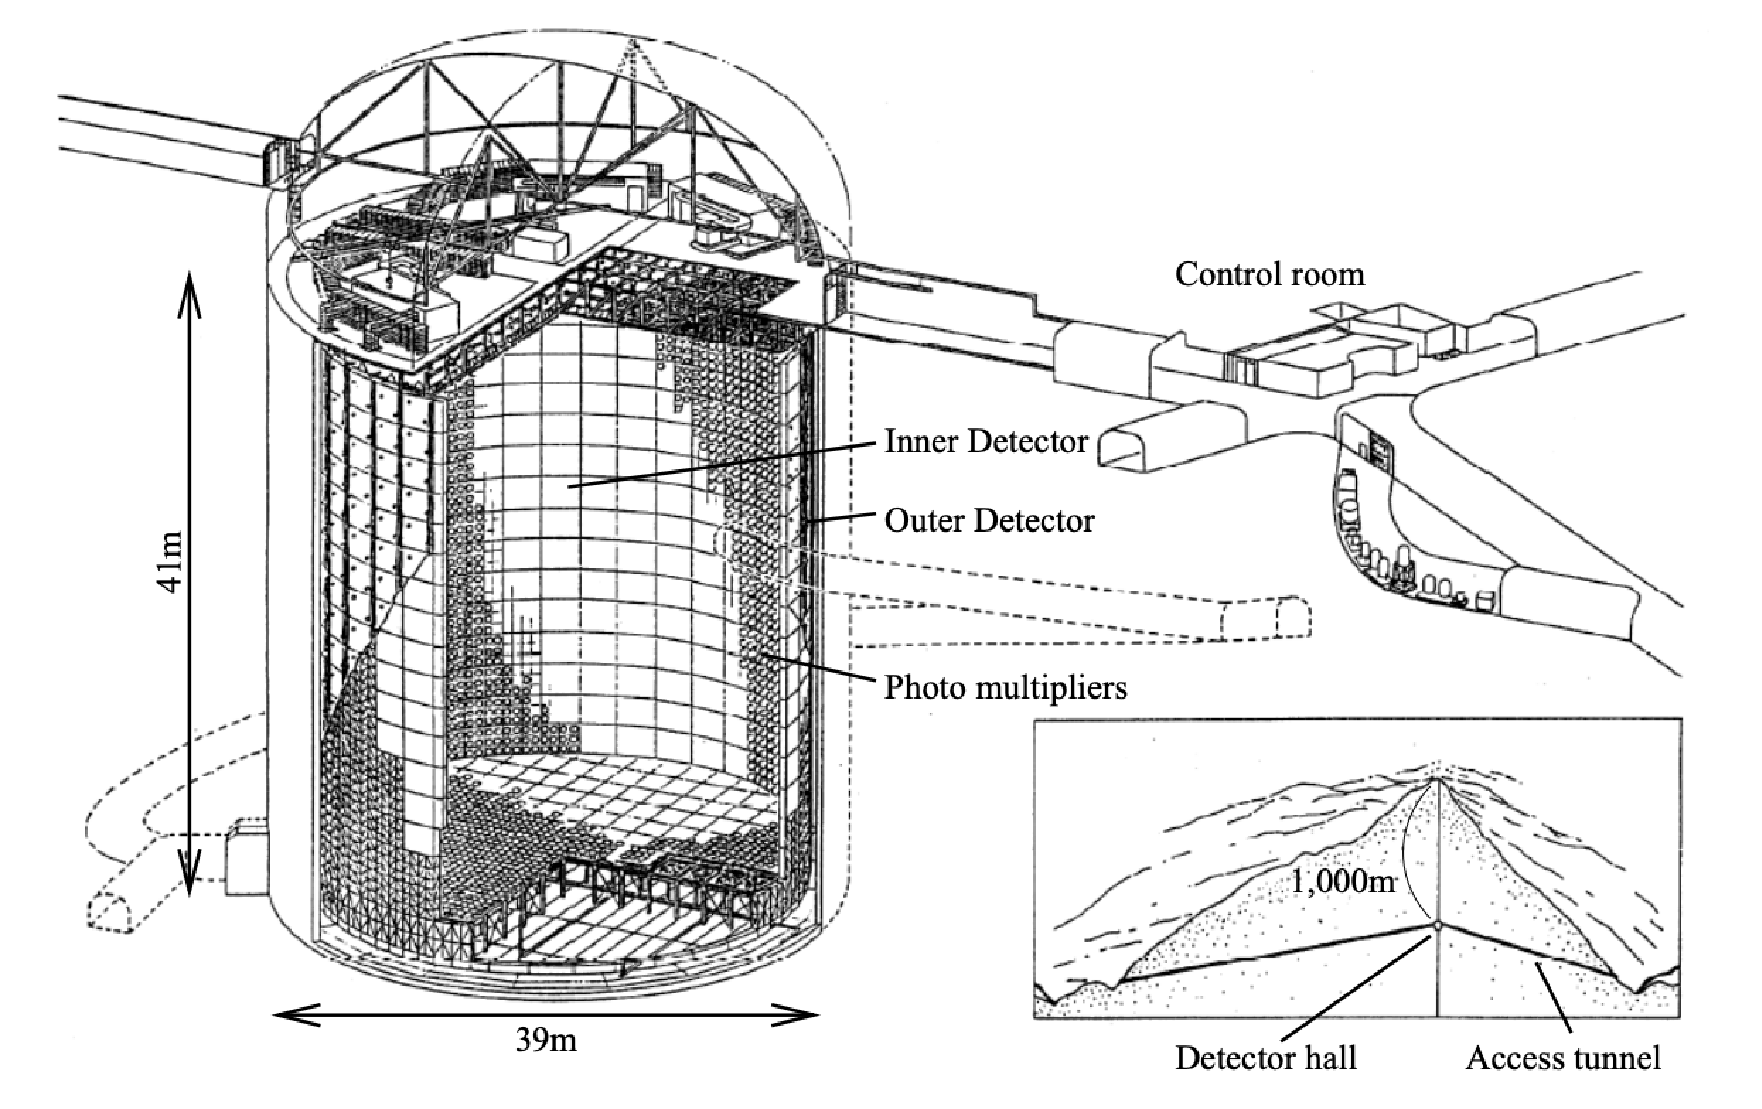
\includegraphics[width=\textwidth, trim={0mm 0mm 0mm 0mm}, clip,page=1]{Figures/Detectors/SKDiagram.pdf}
  \end{subfigure}
  \caption{A schematic diagram of the Super-Kamiokande Detector. Taken from \cite{Itow2001-bc}.}
  \label{fig:T2KSKExp_SK_Diag}
\end{figure}

A smaller cylindrical structure (\quickmath{36.2\text{m}} diameter, \quickmath{33.8\text{m}} height) is situated inside the tank, with an approximate \quickmath{2\text{m}} gap between this structure and the outer tank wall. The purpose of this structure is to support the photomultiplier tubes (PMTs). The volume inside and outside the support structure is referred to as the inner detector (ID) and outer detector (OD), respectively. In the SK-IV era, the ID and OD are instrumented by \quickmath{11,129} \quickmath{50\text{cm}} and \quickmath{1,885} \quickmath{20 \text{cm}} PMTs respectively \cite{Abe_2014_SKCalib}. The ID contains a \quickmath{32\text{kton}} mass of water. Many analyses performed at SK use a ``fiducial volume'' defined by the volume of water inside the ID excluding some distance to the ID wall. This reduces the volume of the detector which is sensitive to neutrino events but reduces radioactive backgrounds and allows for better reconstruction performance. The nominal fiducial volume is defined as the area contained inside \quickmath{2\text{m}} from the ID wall for a total of \quickmath{22.5\text{kton}} water \cite{Jiang2019-iw}.

The two regions of the detector (ID and OD) are optically separated with opaque black plastic hung from the support structure. The purpose of this is to determine whether an event entered or exited the ID. This allows cosmic ray muons and partially contained events to be tagged and separated from neutrino events entirely contained within the ID. This black plastic is also used to cover the area between the ID PMTs to reduce photon reflection from the ID walls. Opposite to this, the OD is lined with a reflective material to allow photons to reflect around inside the OD until collected by one of the PMTs. Furthermore, each OD PMT is optically coupled with \quickmath{50\times50\text{cm}} plates of wavelength shifting acrylic which increases the efficiency of light collection \cite{Fukuda2003-ly}.

In the SK-IV data-taking period, the photocathode coverage of the detector, or the fraction of the ID wall instrumented with PMTs, is \quickmath{\sim 40\%} \cite{Fukuda2003-ly}. The PMTs have a quantum efficiency (the ratio of detected electrons to incident photons) of \quickmath{\sim 21\%} for photons with wavelengths of \quickmath{360\text{nm} < \lambda < 390\text{nm}} \cite{Suzuki1993}. The proportion of photoelectrons that produce a signal in the dynode of a PMT, termed the collection efficiency, is \quickmath{>70 \%} \cite{Fukuda2003-ly}. The PMTs used within SK are most sensitive to photons with wavelength \quickmath{300\text{nm} \leq \lambda \leq 600\text{nm}} \cite{Fukuda2003-ly}. One disadvantage of using PMTs as the detection media is that the Earth's geomagnetic field can modify its response. Therefore, a set of compensation coils is built around the inner surface of the detector to mitigate this effect \cite{t2k_sk}.

As mentioned, the SK detector is filled with ultrapure water, which in a perfect world would contain no impurities. However, bacteria and organic compounds can significantly degrade the water quality. This decreases the attenuation length, which reduces the total number of photons that hit a PMT. To combat this, a sophisticated water treatment system has been developed \cite{Fukuda2003-ly, Nakano2020-sb}. UV lights, mechanical filters, and membrane degasifiers are used to reduce the bacteria, suspended particulates, and radioactive materials from the water. The flow of water within the tank is also critical as it can remove stagnant bacterial growth or build-up of dust on the surfaces within the tank. Gravity drifts impurities in the water towards the bottom of the tank which, if left uncontrolled, can create asymmetric water conditions between the top and bottom of the tank.
%The flow of water in the tank can be controlled via mechanically driven circulation or temperature driven convection.
Typically, the water entering the tank is cooled below the ambient temperature of the tank to control convection and inhibit bacteria growth. Furthermore, the rate of dark noise hits within PMTs is sensitive to the PMT temperature \cite{HamamatsuPMT} so controlling the temperature gradients within the tank is beneficial for stable measurements.

SK-VI is the first phase of the SK experiment to use gadolinium dopants within the ultrapure water \cite{10.5281/zenodo.6694761}. As such, the SK water system had to be replaced to avoid removing the gadolinium concentrate from the ultrapure water \cite{Abe2022-qq}. For an inverse \quickmath{\beta}-decay (IBD) interaction in a water target, the emitted neutron is thermally captured on hydrogen. This process releases \quickmath{2.2 \text{MeV}} \quickmath{\gamma} ray which are difficult to detect as the resulting Compton scattered electrons are very close to the Cherenkov threshold, limiting detection capability. Thermal capture of neutrons on gadolinium generates \quickmath{\gamma} rays with higher energy (\quickmath{8\text{MeV}} \cite{Abe2022-ij}) meaning they are more easily detected and reconstructed. SK-VI has \quickmath{0.01 \%} Gd loading (\quickmath{0.02\%} gadolinium sulphate by mass) which causes \quickmath{\approx 50\%} of neutrons emitted by IBD to be captured on gadolinium\cite{PhysRevLett.93.171101,Marti2020-le} . Whilst predominantly useful for low energy analyses, Gd loading allows better \quickmath{\nu/\bar{\nu}} separation for atmospheric neutrino event selections \cite{Marti2019-gu}. Efforts are currently in place to increase the gadolinium concentrate to \quickmath{0.03 \%} for \quickmath{\approx 75\%} neutron capture efficiency on gadolinium \cite{Vagins2022-sj}. The final stage of loading targets \quickmath{0.1 \%} concentrate targeting \quickmath{\approx 90\%} neutron capture efficiency on gadolinium.

\subsection{Calibration}
\label{subsec:T2KSKExp_SKCalibration}

The calibration of the SK detector is documented in \cite{Abe_2014_SKCalib} and summarised below. The analysis presented within this thesis is dependent upon `high energy events' (Charged particles with \quickmath{O(>100)\text{MeV}} momenta). These are events that are expected to generate a larger number of photons such that each PMT will be hit with multiple photons. The reconstruction of these events depends upon the charge deposited within each PMT and the timing response of each individual PMT. Therefore, the most relevant calibration techniques to this thesis are outlined.

Before installation, \quickmath{420} PMTs were calibrated to have identical charge responses and then distributed throughout the tank in a cross-shape pattern (As illustrated by \autoref{fig:T2KSKExp_SK_StandardPMTs}). These are used as a standardised measure for the rest of the PMTs installed at similar geometric positions within SK to be calibrated against.
%This allows each PMT to have it's high voltage set so that all PMTs give the same signal for an identical light collection.
To perform this calibration, a xenon lamp is located at the centre of the SK tank which flashes uniform light at \quickmath{1 \text{Hz}}. This allows for geometrical effects, water quality variation, and timing effects to be measured in-situ throughout normal data-taking periods.

\begin{figure}[h]
  \begin{subfigure}[t]{0.50\textwidth}
    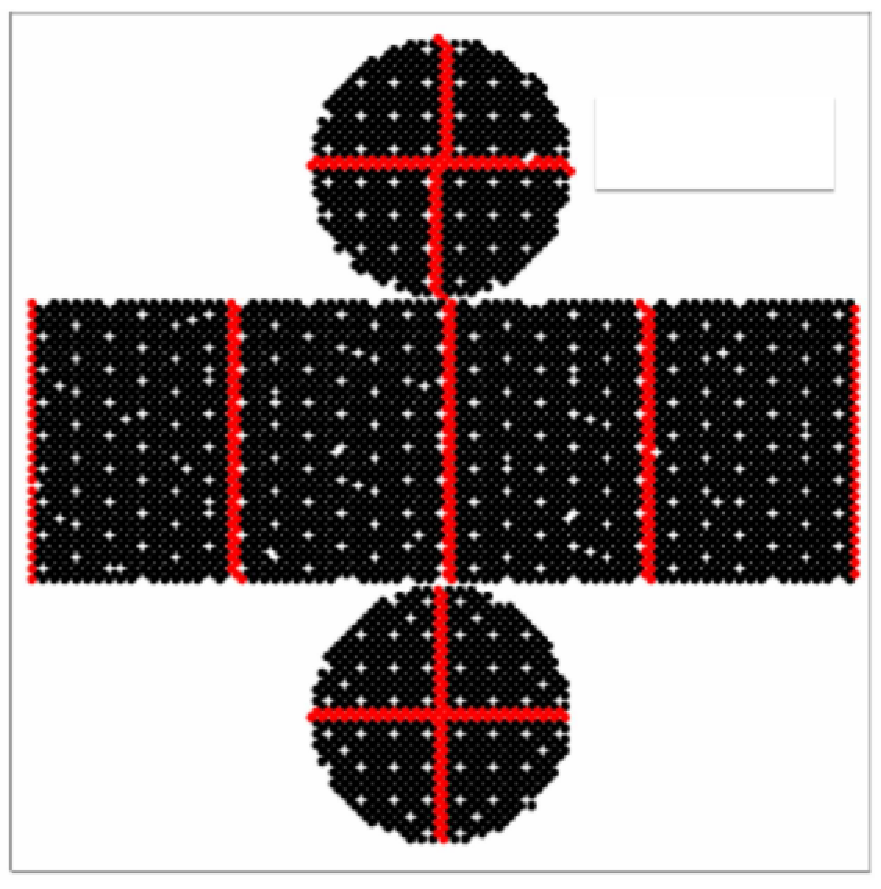
\includegraphics[width=\textwidth, trim={0mm 0mm 0mm 0mm}, clip,page=1]{Figures/Detectors/StandardPMTs.pdf}
  \end{subfigure}
  \caption{The location of ``standard PMTs'' (red) inside the SK detector. Taken from \cite{Abe_2014_SKCalib}.}
  \label{fig:T2KSKExp_SK_StandardPMTs}
\end{figure}

When specifically performing calibration of the detector (in out-of-data taking mode), the water in the tank was circulated to avoid top/bottom asymmetric water quality. Any non-uniformity within the tank significantly affects the PMT hit probability through scattering or absorption. This becomes a dominant effect for the very low-intensity light sources discussed later which are designed such that only one photon is incident upon a given PMT.

The ``gain'' of a PMT is defined as the ratio of the total charge of the signal produced compared to the charge of photoelectrons emitted by the photocathodes within the PMT. To calibrate the signal of each PMT, the ``relative'' and ``absolute'' gain values are measured. The relative gain is the variation of gain among each of the PMTs whereas the absolute gain is the average gain of all PMTs. 

The relative gain is calibrated as follows. A laser is used to generate two measurements: a high-intensity flash that illuminates every PMT with a sufficient number of photons, and a low-intensity flash in which only a small number of PMTs collect light. The first measurement creates an average charge, \quickmath{Q_{obs}(i)} on PMT \quickmath{i}, whereas the second measurement ensures that each hit PMT only generates a single photoelectron. For the low-intensity measurement, the number of times each PMT records a charge larger than \quickmath{1/4} photoelectrons, \quickmath{N_{obs}(i)}, is counted. The values measured can be expressed as

\begin{equation}
  \label{eq:T2KSKExp_RelativeGainCalib}
  \begin{split}
    Q_{obs}(i) &\propto I_{H} \times f(i) \times \epsilon(i) \times G(i), \\
    N_{obs}(i) &\propto I_{L} \times f(i) \times \epsilon(i),
  \end{split}
\end{equation}

Where \quickmath{I_{H}} and \quickmath{I_{L}} is the intensity of the high and low flashes, \quickmath{f(i)} is the acceptance efficiency of the \quickmath{i^{\text{th}}} PMT, \quickmath{\epsilon(i)} is the product of the quantum and collection efficiency of the \quickmath{i^{\text{th}}} PMT and \quickmath{G(i)} is the gain of the \quickmath{i^{\text{th}}}	PMT. The relative gain for each PMT can determined by taking the ratio of these quantities.

The absolute gain calibration is performed by observing fixed energy \quickmath{\gamma}-rays of \quickmath{E_{\gamma} \sim 9\text{MeV}} emitted isotropically from neutron capture on a NiCf source situated at the centre of the detector. This generates a photon yield of about \quickmath{0.004} photoelectrons/PMT/event, meaning that \quickmath{>99\%} of PMT signals are generated from single photoelectrons. A charge distribution is generated by performing this calibration over all PMTs, and the average value of this distribution is taken to be the absolute gain value.
%It has been found that the absolute gain increases as a function of time despite there being no known reason for this behaviour.

As mentioned in \autoref{subsec:T2KSKExp_SKDetector}, the average quantum and collection efficiency for the SK detector PMTs is \quickmath{\sim 21\%} and \quickmath{>70 \%} respectively. However, these values do differ between each PMT and need to be calibrated accordingly. Consequently, the NiCf source is also used to calibrate the ``quantum \quickmath{\times} collection'' efficiency (denoted ``QE'') value of each PMT.
%This value is calculated as calibrating the signal generated by one incident photon is of more importance than the individual efficiency of photoelectron emission or detection on the dynode.
The NiCf low-intensity source is used as the PMT hit probability is proportional to the QE (\quickmath{N_{obs}(i) \propto \epsilon(i)} in \autoref{eq:T2KSKExp_RelativeGainCalib}). A Monte Carlo prediction which includes photon absorption, scattering, and reflection is made to estimate the number of photons incident on each PMT and the ratio of the number of predicted to observed hits is calculated. The difference is attributed to the QE efficiency of that PMT. This technique is extended to calculate the relative QE efficiency by normalizing the average of all PMTs which removes the dependence on the light intensity.

Due to differing cable lengths and readout electronics, the timing response between a photon hitting the PMT and the signal being captured by the data acquisition can be different between each PMT. Due to threshold triggers (Described in \autoref{subsec:T2KSKExp_SKTriggering}), the time at which a pulse reaches a threshold is dependent upon the size of the pulse. This is known as the `time-walk' effect and also needs to be accounted for in each PMT. To calibrate the timing response, a pulse of light with width \quickmath{0.2\text{ns}} is emitted into the detector through a diffuser. Two-dimensional distributions of time and pulse height (or charge) are made for each PMT and are used to calibrate the timing response. This is performed in-situ during data taking with the light source pulsing at \quickmath{0.03\text{Hz}}.

The top/bottom water quality asymmetry is measured using the NiCf calibration data and cross-referencing these results to the ``standard PMTs''. The water attenuation length is continuously measured by the rate of vertically-downgoing cosmic-ray muons which enter via the top of the tank.

%In the ultra-relativistic approximation that \quickmath{\beta=1}, a charged particle will generate Cherenkov photons with a characteristic pitch angle of \quickmath{42^{\circ}}. By calculating the ratio of the charge deposited on PMTs within this cone angle to that outside of the cone, the rate of photon scattering can be calculated. This value is dependent upon the water quality inside the tank. Performing this calculation using cosmic ray muons allows the water quality to be monitored in real time. A more complex analysis, which uses a collimated laser to inject photons at different wavelengths is performed to determine the Rayleigh scattering, Mie scattering and absorption coefficients. This methodology divides the tank into five horizontal slices, where the timing and spatial distribution of hits PMTs in each slice can be compared between data and various Monte Carlo predictions. The coefficients which minimise the \quickmath{\chi^2} between data and Monte Carlo are selected and utilised within the detector simulation.

Dark noise is where a PMT registers a pulse that is consistent with a single photoelectron emitted from photon detection despite the PMT being in complete darkness. This is predominately caused by two processes. Firstly there is intrinsic dark noise which is where photoelectrons gain enough thermal energy to be emitted from the photocathode, and secondly, the radioactive decay of contaminants inside the structure of the PMT. Typical dark noise rate for PMTs used within SK are \quickmath{O(3)\text{kHz}} \cite{Fukuda2003-ly}. This is lower than the expected number of photons generated for a `high energy event' (As described in \autoref{subsec:T2KSKExp_Cherenkov}) but instability in this value can cause biases in reconstruction. Dark noise is related to the gain of a PMT and is calibrated using hits inside a time window recorded before an event trigger \cite{thesis_focht}.

\subsection{Data Acquisition and Triggering}
\label{subsec:T2KSKExp_SKTriggering}

%The maximum distance that a photon can travel within the SK detector is \quickmath{\sim 200\text{ns}} \cite{PhysRevD.73.112001}.
As the analysis presented in this thesis only uses the SK-IV period of the SK experiment so this subsection focuses on the relevant points of the data acquisition and triggering systems to that SK period. The earlier data acquisition and triggering systems are documented in \cite{34489,PhysRevD.73.112001}. 

Before the SK-IV period started, the existing front-end electronics were replaced with ``QTC-Based Electrons with Ethernet, QBEE'' systems \cite{Nishino2009-wh}. When the QBEE observes a signal above a \quickmath{1/4} photoelectron threshold, the charge-to-time (QTC) converter generates a rectangular pulse. The start of the rectangular pulse indicates the time at which the analog photoelectron signal was received and the width of the pulse indicates the total charge integrated throughout the signal. This is then digitized by time-to-digital converters and sent to the ``front-end'' PCs. The digitized signal from every QBEE is then chronologically ordered and sent to the ``merger'' PCs. It is the merger PCs that apply the software trigger. Any triggered events are passed to the ``organizer'' PC. This sorts the data stream of multiple merger PCs into chronologically ordered events which are then saved to disk. The schematic of data flow from PMTs to disk is illustrated in \autoref{fig:T2KSKExp_SK_DataFlow}.

\begin{figure}[h]
  \begin{subfigure}[t]{0.80\textwidth}
    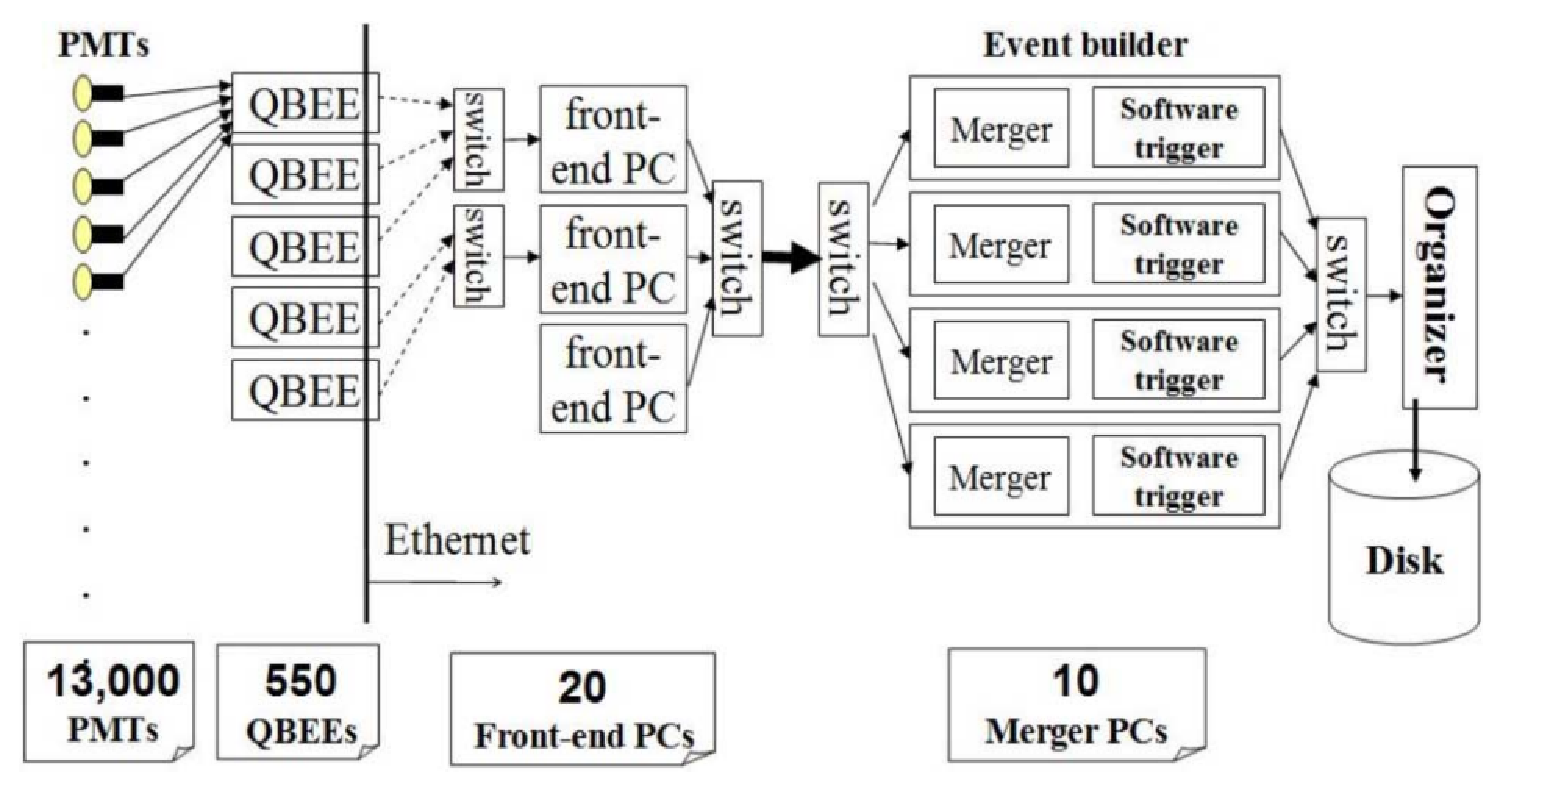
\includegraphics[width=\textwidth, trim={0mm 0mm 0mm 0mm}, clip,page=1]{Figures/Detectors/SKDataFlow.pdf}
  \end{subfigure}
  \caption{Schematic view of the data flow through the data acquisition and online system. Taken from \cite{5446533}.}
  \label{fig:T2KSKExp_SK_DataFlow}
\end{figure}

%The software trigger applied in SK-IV replaces the hardware trigger applied in SK-I to SK-III.
The software trigger (described in \cite{Yamada2007-cp}) operates by determining the number of PMT hits within a \quickmath{200\text{ns}} sliding window, \quickmath{N_{200}}. This window coincides with the maximum time that a Cherenkov photon would take to traverse the length of the SK tank \cite{PhysRevD.73.112001}. For lower energy events that generate fewer photons, this technique is useful for eliminating background processes like dark noise and radioactive decay which would be expected to separate in time. When the value of \quickmath{N_{200}} exceeds some threshold, a software trigger is issued. There are several trigger thresholds used within the SK-IV period which are detailed in \autoref{tab:T2KSKExp_TriggerThreshold}. If one of these thresholds is met, the PMT hits within an extended time window are also read out and saved to disk.
%The length of the time window is also included in the tabulated threshold conditions.
In the special case of an event that exceeds the SHE trigger but does not exceed the OD trigger, the AFT trigger looks for delayed coincidences of \quickmath{2.2 \text{MeV}} gamma rays emitted from neutron capture in a \quickmath{535 \mu\text{s}} window after the SHE trigger. A similar but more complex ``Wideband Intelligent Trigger (WIT)'' has been deployed and is described in \cite{Carminati2015-zx}.

\begin{table}[ht!]
    \centering
    \begin{tabular}{l|c|c|c}
      \hline
      Trigger & Acronym & Condition & Extended time window (\quickmath{\mu \text{s}}) \\
      \hline
      Super Low Energy & SLE & >34/31 hits & 1.3 \\
      Low Energy & LE & >47 hits & 40 \\
      High Energy & HE & >50 hits & 40 \\
      Super High Energy & SHE & >70/58 hits & 40 \\
      Outer Detector & OD & >22 hits in OD & N/A \\
      \hline
      \hline
    \end{tabular}
    \caption{The trigger thresholds and extended time windows saved around an event which were utilised throughout the SK-IV period. The exact thresholds can change and the values listed here represent the thresholds at the start and end of the SK-IV period.}
    \label{tab:T2KSKExp_TriggerThreshold}
\end{table}

\subsection{Cherenkov Radiation}
\label{subsec:T2KSKExp_Cherenkov}

Cherenkov light is emitted from any highly energetic charged particle traveling with relativistic velocity, \quickmath{\beta}, greater than the local speed of light in a medium \cite{Cerenkov1937-tl}.
%with refractive index \quickmath{n>1.0} 
%This occurs due to the charged particle exciting the polarised media, which de-excites via photon emission. From Huygen's principal, the emitted waves propagate outwards but only generate coherent wavefronts when the charged particle moves faster than the phase velocity of that media. Consequently,
Cherenkov light is formed at the surface of a cone with characteristic pitch angle,

\begin{equation}
  \label{eq:T2KSKExp_CherenkovConeAngle}
  \cos(\theta)=\frac{1}{\beta n}.
\end{equation}

where \quickmath{n} is the refractive index of the medium. Consequently, the Cherenkov momentum threshold, \quickmath{P_{thres}}, is dependent upon the mass, \quickmath{m}, of the charged particle moving through the medium, 

\begin{equation}
  P_{thres} = \frac{m}{\sqrt{n^{2}-1}}
\end{equation}

For water, where \quickmath{n = 1.33}, the Cherenkov threshold momentum and energy for various particles are given in \autoref{tab:T2KSKExp_CherenkovThreshold}. In contrast, \quickmath{\gamma}-rays are detected indirectly via the combination of photons generated by Compton scattering and pair production. The threshold for detection in the SK detector is typically higher than the threshold for photon production. This is due to the fact that the attenuation of photons in the water means that typically \quickmath{\sim 75\%} of Cherenkov photons reach the ID PMTs. Then the collection and quantum efficiencies described in \autoref{subsec:T2KSKExp_SKDetector} result in the number of detected photons being lower than the number of photons which reach the PMTs. 

\begin{table}[ht!]
    \centering
    \begin{tabular}{l|c|c}
      \hline
      Particle & Threshold Momentum (MeV) & Threshold Energy (MeV)\\
      \hline
      Electron & 0.5828 & 0.7751 \\
      Muon & 120.5 & 160.3 \\
      Pion & 159.2 & 211.7 \\
      Proton & 1070.0 & 1423.1 \\
      \hline
      \hline
    \end{tabular}
    \caption{The threshold momentum and energy for a particle to generate Cherenkov light in ultrapure water, as calculated in \autoref{eq:T2KSKExp_CherenkovConeAngle} in ultrapure water which has refractive index \quickmath{n = 1.33}.}
    \label{tab:T2KSKExp_CherenkovThreshold}
\end{table}

The Frank-Tamm equation \cite{Frank1991-wj} describes the relationship between the number of Cherenkov photons generated per unit length, \quickmath{dN/dx}, the wavelength of the photons generated, \quickmath{\lambda}, and the relativistic velocity of the charged particle,

\begin{equation}
  \label{eq:T2KSKExp_FrankTammFormula}
  \frac{d^2N}{dxd\lambda} = 2\pi\alpha \left(1 - \frac{1}{n^2 \beta^2} \right)\frac{1}{\lambda^2} .
\end{equation}

where \quickmath{\alpha} is the fine structure constant. For a \quickmath{100\text{MeV}} momentum electron, approximately \quickmath{330} photons will be produced per centimeter in the \quickmath{300\text{nm} \leq \lambda \leq 700\text{nm}} region which the ID PMTs are most sensitive to \cite{Fukuda2003-ly}.

\section{The Tokai to Kamioka Experiment}
\label{sec:T2KSKExp_T2K}

The Tokai to Kamioka (T2K) experiment is a long-baseline neutrino oscillation experiment located in Japan. Proposed in the early 2000s \cite{jhf_loi, Itow2001-vw} to replace K2K \cite{The_K2K_Collaboration2001-oo}, T2K was designed to observe electron neutrino appearance whilst precisely measuring the oscillation parameters associated with muon neutrino disappearance \cite{t2k_proposal}. The experiment consists of a neutrino beam generated at the Japan Proton Accelerator Research Complex (J-PARC), a suite of near detectors situated \quickmath{280\text{m}} from the beam target, and the Super Kamiokande far detector positioned at a \quickmath{295\text{km}} baseline. The cross-section view of the T2K experiment is drawn in \autoref{fig:T2KSKExp_T2K_Overview}.

\begin{figure}[h]
  \begin{subfigure}[t]{0.95\textwidth}
    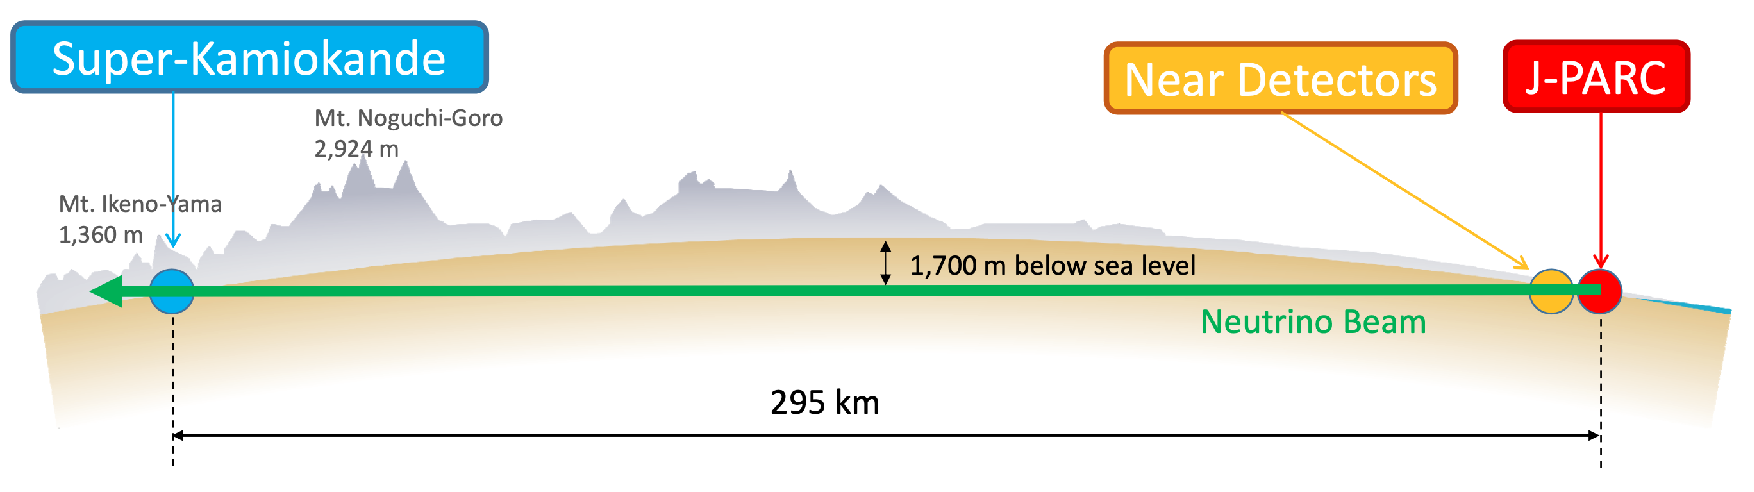
\includegraphics[width=\textwidth, trim={0mm 0mm 0mm 0mm}, clip,page=1]{Figures/Detectors/T2KCrossSection.pdf}
  \end{subfigure}
  \caption{The cross-section view of the Tokai to Kamioka experiment illustrating the beam generation facility at J-PARC, the near detector situated at a baseline of \quickmath{280\text{m}} and the Super Kamiokande far detector situated \quickmath{295\text{km}} from the beam target.}
  \label{fig:T2KSKExp_T2K_Overview}
\end{figure}

The T2K collaboration makes world-leading measurements of the \sinsqatm, \delmsqatm, and \dcp oscillation parameters. Improvements in the precision and accuracy of parameter estimates are still being made by including new data samples and developing the models which describe the neutrino interactions and detector responses \cite{Bronner2022-wd}. Electron neutrino appearance was first observed at T2K in 2014 \cite{2014_Abe_ElectronNuApp} with \quickmath{7.3\sigma} significance.

The near detectors provide constraints on the beam flux and cross-section model parameters used within the oscillation analysis by observing the unoscillated neutrino beam. There are a host of detectors situated in the near detector hall (As illustrated in \autoref{fig:T2KSKExp_T2K_ND280Pit}): ND280 (\autoref{subsec:T2KSKExp_T2K_ND280}), INGRID (\autoref{subsec:T2KSKExp_T2K_INGRID}), NINJA \cite{ninja}, WAGASCI \cite{wagasci}, and Baby-MIND \cite{baby_mind}. The latter three are not currently used within the oscillation analysis presented within this thesis.

\begin{figure}[h]
  \begin{subfigure}[t]{0.5\textwidth}
    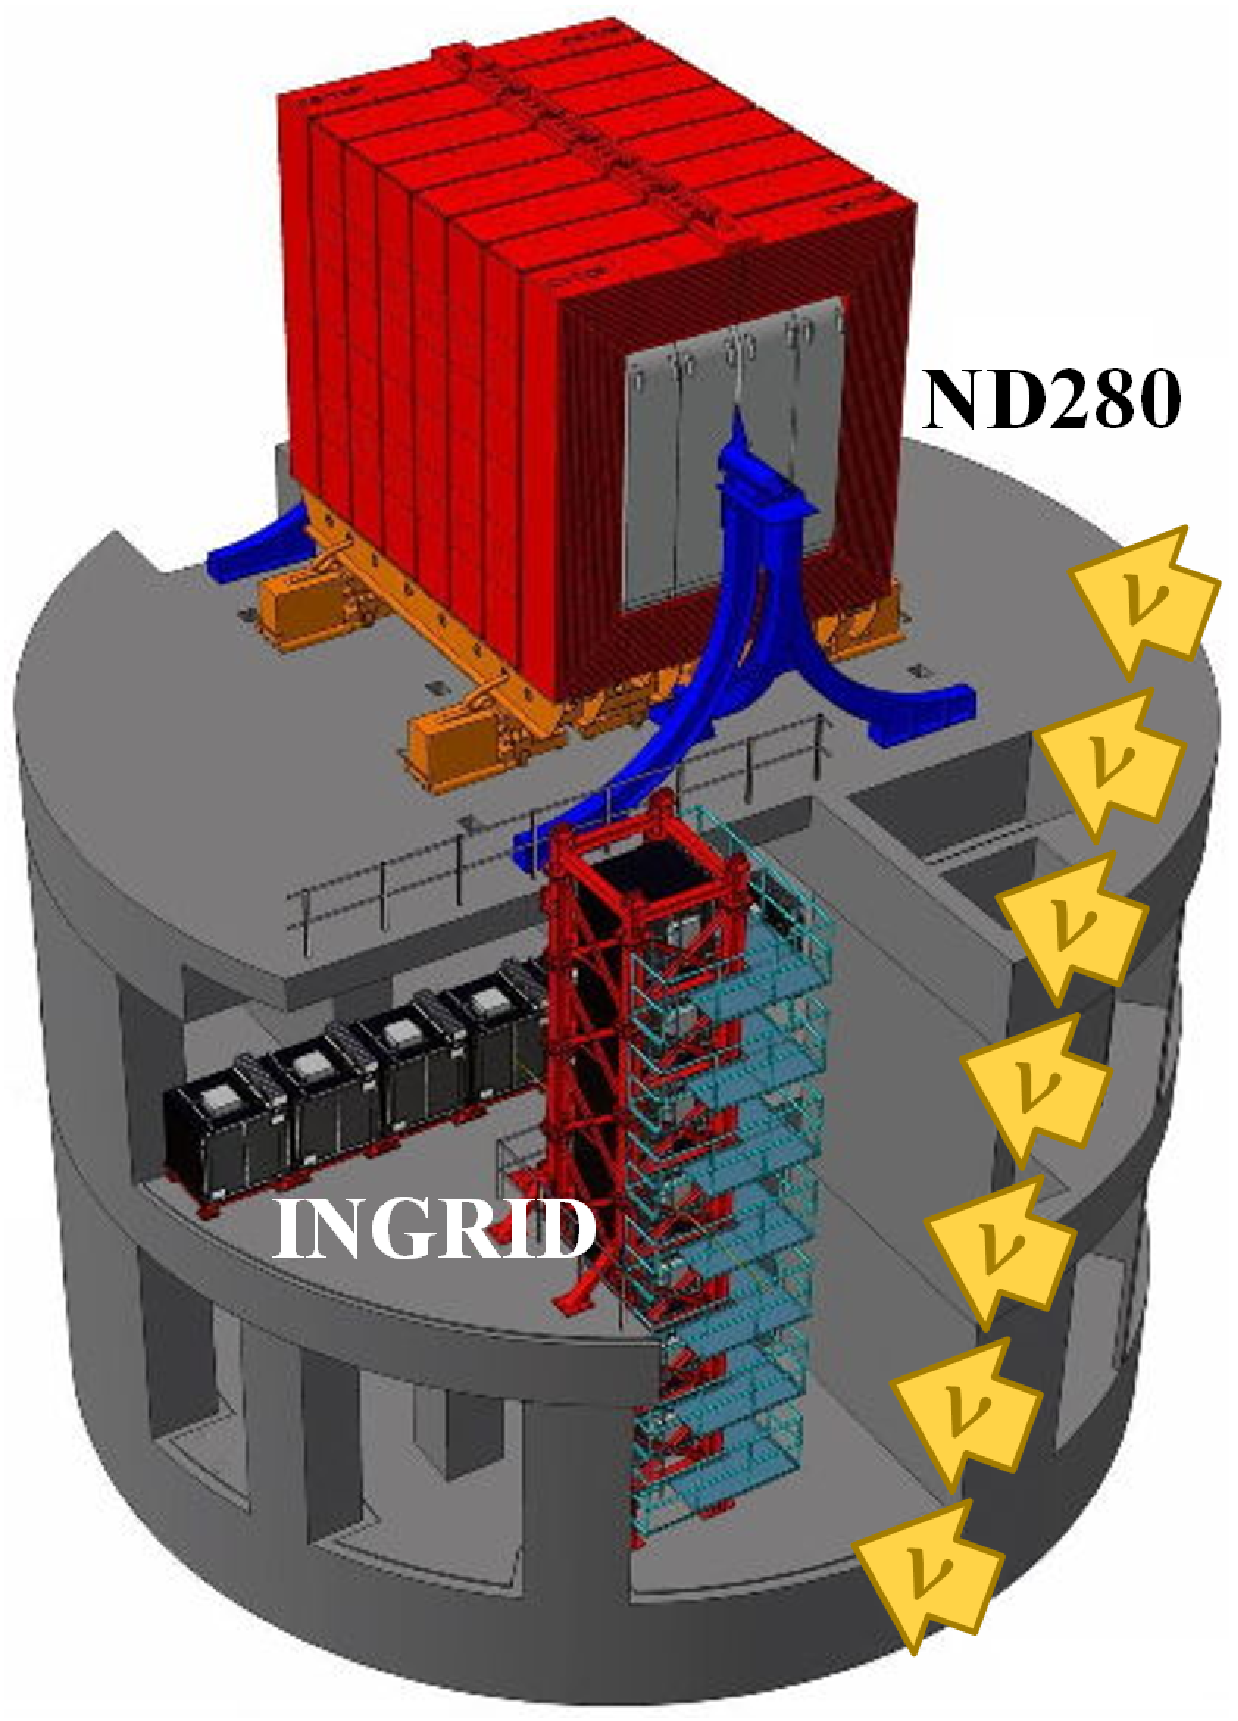
\includegraphics[width=\textwidth, trim={0mm 0mm 0mm 0mm}, clip,page=1]{Figures/Detectors/T2KND280Hall.pdf}
  \end{subfigure}
  \caption{The near detector suite for the T2K experiment showing the ND280 and INGRID detectors. The distance between the detectors and the beam target is \quickmath{280\text{m}}.}
  \label{fig:T2KSKExp_T2K_ND280Pit}
\end{figure}

Whilst this thesis presents the ND280 in terms of its purpose for the oscillation analysis, the detector can also make many cross-section measurements at neutrino energies of \quickmath{O(1)\text{GeV}} for the different targets within the detector \cite{PhysRevD.102.012007,10.1093/ptep/ptab014}. These measurements are of equal importance as they can lead the way in determining the model parameters used in the interaction models for the future high-precision era of neutrino physics.

There are two independent fitters, \texttt{MaCh3} and \texttt{BANFF}, which perform the near detector fit. \texttt{MaCh3} is the basis of this analysis and uses a bayesian Markov Chain Monte Carlo fitting technique, whereas \texttt{BANFF} uses a frequentist gradient descent technique. The output of each fitter is converted into a covariance matrix to describe the error and correlations between all the flux and cross-section parameters. This is then propagated to the far-detector oscillation analysis group for use in the \texttt{P-Theta} and \texttt{VALOR} fitting framework. As \texttt{MaCh3} can handle both near and far detector samples, it does not use this covariance matrix and instead opts for a simultaneous fit of the two detector measurements. This is an analysis choice which removes the assumption of Gaussian posterior distributions required when building the post-fit covariance matrix.

\finish{MaCh3 vs PTheta and Valor}

There are three particular tunes of the T2K flux and low energy cross section model typically considered. Firstly, the ``generated'' tune which is the set of dial values with which the Monte Carlo was generated. Secondly, the set of dial values which are taken from external data measurements and used as inputs. These are the ``pre-fit'' dial values. The reason these two sets of dial values are different is that the external data measurements are continually updated but it is very computationally intensive to regenerate a Monte Carlo prediction after each update. The final tune is the ``post-fit'', ``post-ND fit'' or ``post-BANFF'' dial values. These are the values taken from the fit to the beam near detector data.

\subsection{The Neutrino Beam}
\label{subsec:T2KSKExp_T2K_NeutrinoBeam}

The neutrino beam used within the T2K experiment is described in \cite{t2k_det, Abe_2013} and summarised below. The accelerating facility at J-PARC is composed of two sections; the primary and secondary beamlines. \autoref{fig:T2KSKExp_T2K_Beamline} illustrates a schematic of the beamline, focusing mostly on the components of the secondary beamline. The primary beamline has three accelerators that progressively accelerate protons; a linear accelerator, a rapid-cycling synchrotron, and the main-ring (MR) synchrotron. Once fully accelerated by the MR, the protons have a kinetic energy of \quickmath{30\text{GeV}}. Eight bunches of these protons, separated by \quickmath{500\text{ns}}, are extracted per ``spill'' from the MR and directed towards a graphite target (a rod of length \quickmath{91.4\text{cm}} and diameter \quickmath{2.6\text{cm}}).
Spills are extracted at \quickmath{~0.5\text{Hz}} with \quickmath{\sim 3\times10^{14}} protons contained per spill.
%A total of \quickmath{\sim 3\times 10^{14}} protons are contained in each spill. The rate of extracted spills is \quickmath{\sim 0.5\text{Hz}} although the width of the spill is \quickmath{\sim 5 \mu\text{s}}.

\begin{figure}[h]
  \begin{subfigure}[t]{0.7\textwidth}
    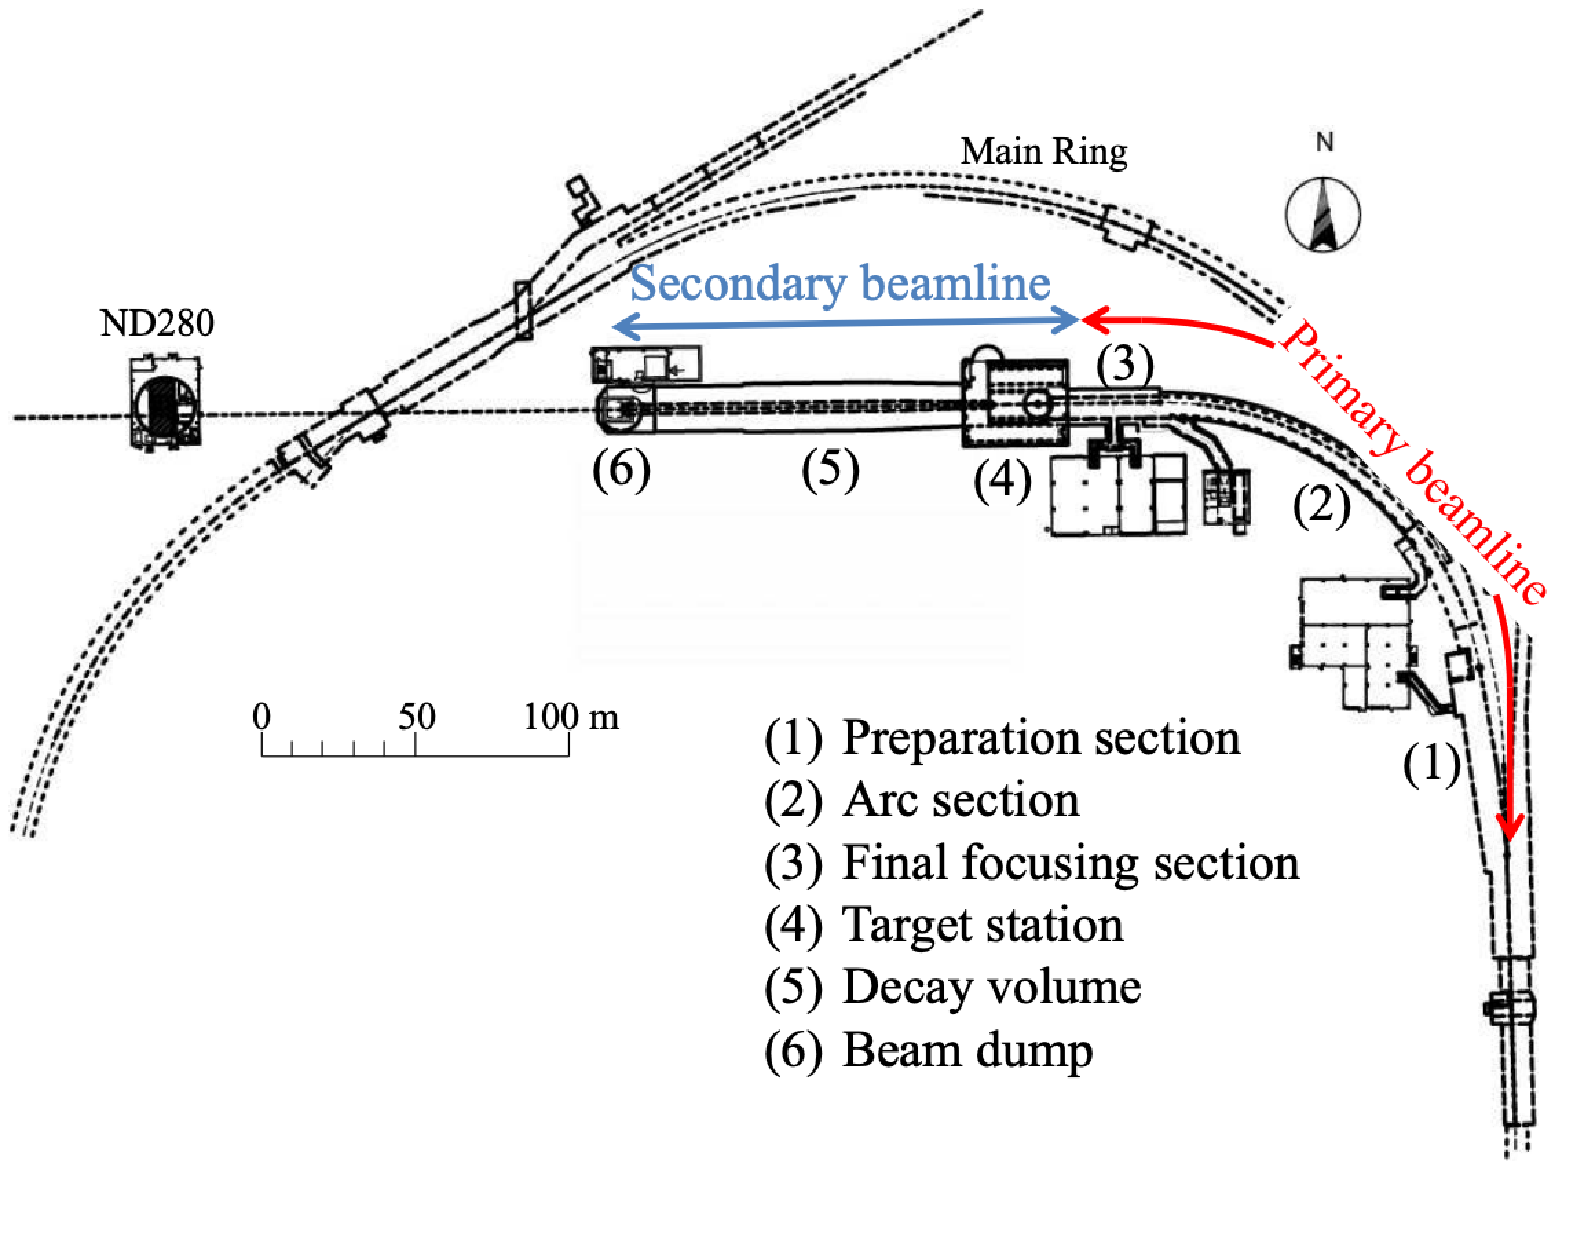
\includegraphics[width=\textwidth, trim={0mm 0mm 0mm 0mm}, clip,page=1]{Figures/Detectors/T2KBeamline.pdf}
    \subcaption{Primary and secondary beamline}
  \end{subfigure}
  \begin{subfigure}[t]{0.95\textwidth}
    \vspace{0.5cm}
    \includegraphics[width=\textwidth, trim={0mm 0mm 0mm 0mm}, clip,page=1]{Figures/Detectors/T2KSecondaryBeamline.pdf}
    \subcaption{Secondary beamline}
  \end{subfigure}
  \caption{Top panel: Bird's eye view of the most relevant part of primary and secondary beamline used within the T2K experiment. The primary beamline is the main-ring proton synchrotron, kicker magnet, and graphite target. The secondary beamline consists of the three focusing horns, decay volume, and beam dump. Figure taken from \cite{t2k_det}. Bottom panel: The side-view of the secondary beamline including the focusing horns, beam dump and neutrino detectors. Figure taken from \cite{MuMon}.}
  \label{fig:T2KSKExp_T2K_Beamline}
\end{figure}

The secondary beamline consists of three main components: the target station, the decay volume, and the beam dump. The target station is comprised of the target, beam monitors, and three magnetic focusing horns. The proton beam interacts with the graphite target to form a secondary beam of mostly pions and kaons. The secondary beam travels through a \quickmath{96\text{m}} long decay volume, generating neutrinos through the following decays \cite{Abe_2013},

\begin{minipage}{.45\linewidth}
  \begin{equation}
    \begin{split}
      \pi^+ &\rightarrow \mu^+ + \nu_\mu \\
      K^+ &\rightarrow \mu^+ + \nu_\mu \\
      &\rightarrow \pi^0 + e^+ + \nu_e \\
      &\rightarrow \pi^0 + \mu^+ + \nu_\mu \\
      K^0_L &\rightarrow \pi^- + e^+ + \nu_e \\
      &\rightarrow \pi^- + \mu^+ + \nu_\mu \\
      \mu^+ &\rightarrow e^+ + \bar{\nu}_\mu + \nu_e  \notag
    \end{split}
  \end{equation}
\end{minipage}%
\begin{minipage}{.45\linewidth}
  \begin{equation}
    \begin{split}
      \pi^- &\rightarrow \mu^- + \bar{\nu}_\mu\\
      K^- &\rightarrow \mu^- + \bar{\nu}_\mu \\
      &\rightarrow \pi^0 + e^- + \bar{\nu}_e\\
      &\rightarrow \pi^0 + \mu^- + \bar{\nu}_\mu \\
      K^0_L &\rightarrow \pi^+ + e^- + \bar{\nu}_e \\
      &\rightarrow \pi^+ + \mu^- + \bar{\nu}_\mu \\
      \mu^- &\rightarrow e^- + \nu_\mu + \bar{\nu}_e  \notag
    \end{split}
  \end{equation}
\end{minipage}

The electrically charged component of the secondary beam is focused towards the far detector by the three magnetic horns. These horns direct charged particles of a particular polarity towards SK whilst defocusing the oppositely charged particles. This allows a mostly neutrino or mostly antineutrino beam to be used within the experiment, denoted as ``forward horn current (FHC)'' or ``reverse horn current (RHC)'' respectively.

\autoref{fig:T2KSKExp_T2K_NuFluxPerMode} illustrates the different contributions to the FHC and RHC neutrino flux. The low energy flux is dominated by the decay of pions whereas kaon decay becomes the dominant source of neutrinos for \quickmath{E_\nu > 3\text{GeV}}. The ``wrong-sign'' component, which is the \quickmath{\bar{\nu}_\mu} background in a \quickmath{\nu_\mu} beam, and the intrinsic irreducible \quickmath{\nu_e} background, are predominantly due to muon decay for \quickmath{E_\nu < 2\text{GeV}}. As the antineutrino production cross-section is smaller than the neutrino cross-section, the wrong-sign component is more dominant in the RHC beam as compared to that in the FHC beam.

\begin{figure}[h]
  \begin{subfigure}[t]{0.45\textwidth}
    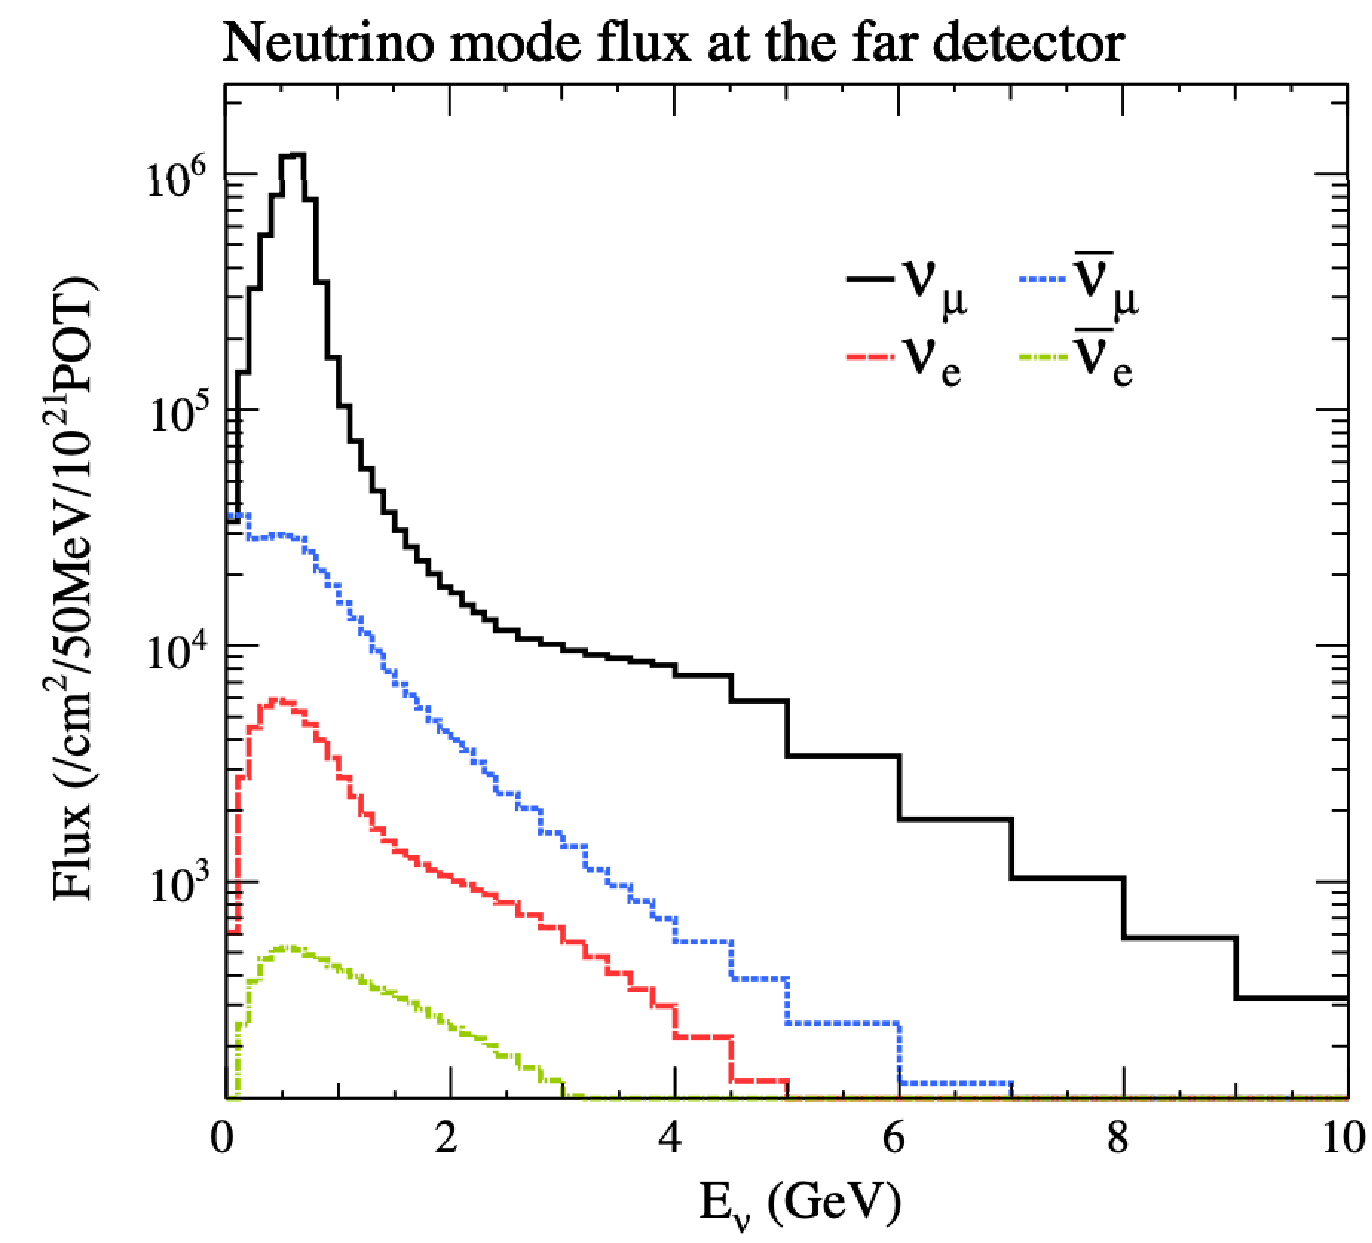
\includegraphics[width=\textwidth, trim={0mm 0mm 0mm 0mm}, clip,page=1]{Figures/Detectors/T2KFluxInNuMode.pdf}
  \end{subfigure}%
  \begin{subfigure}[t]{0.45\textwidth}
    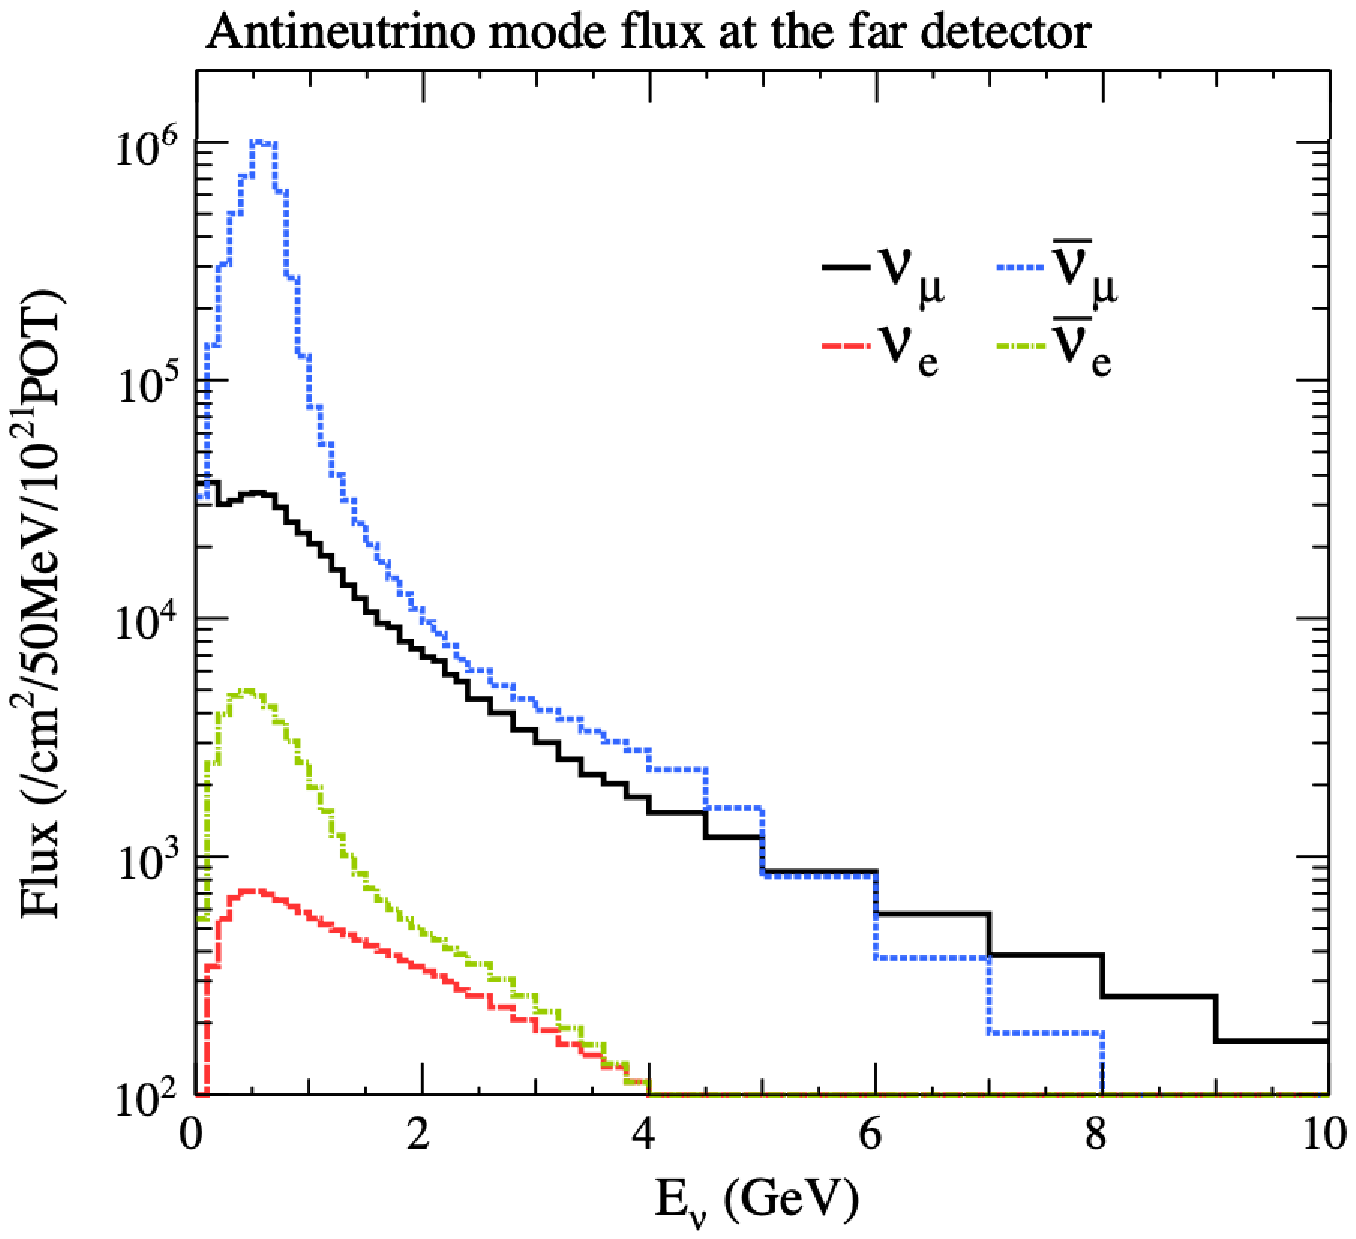
\includegraphics[width=\textwidth, trim={0mm 0mm 0mm 0mm}, clip,page=1]{Figures/Detectors/T2KFluxInANuMode.pdf}
  \end{subfigure}
  \caption{The Monte Carlo prediction of the energy spectrum for each flavour of neutrino (\quickmath{\nu_e}, \quickmath{\bar{\nu}_e}, \quickmath{\nu_\mu} and \quickmath{\bar{\nu}_\mu}) in the neutrino dominated beam FHC mode (Left) and antineutrino dominated beam RHC mode (Right) expected at SK. Taken from \cite{Abe2021-tr}.}
  \label{fig:T2KSKExp_T2K_NuFluxPerMode}
\end{figure}

The beam dump, situated at the end of the decay volume, stops all charged particles other than highly energetic muons (\quickmath{p_\mu > 5\text{GeV}}). The MuMon detector monitors the penetrating muons to determine the beam direction and intensity which is used to constrain some of the beam flux systematics within the analysis \cite{MuMon, Vladisavljevic2020-gv}. 

The T2K experiment uses an off-axis beam to narrow the neutrino energy distribution. This was the first implementation of this technique in a long-baseline neutrino oscillation experiment after its original proposal \cite{Beavis1995-qf}. Pion decay, \quickmath{\pi \rightarrow \mu + \nu_\mu}, is a two-body decay. Consequently, the neutrino energy, \quickmath{E_\nu}, can be determined based on the pion energy, \quickmath{E_\pi}, and the angle at which the neutrino is emitted, \quickmath{\theta},

\begin{equation}
  E_\nu = \frac{m^{2}_{\pi} - m^{2}_{\mu}}{2\left(E_\pi - p_\pi \cos(\theta) \right)},
\end{equation}

where \quickmath{m_{\pi}} and \quickmath{m_{\mu}} are the mass of the pion and muon respectively. For a fixed energy pion, the neutrino energy distribution is dependent upon the angle at which the neutrinos are observed from the initial pion beam direction. For the \quickmath{295\text{km}} baseline at T2K, \quickmath{E_\nu = 0.6\text{GeV}} maximises the electron neutrino appearance probability, \quickmath{P(\nu_\mu \rightarrow \nu_e)}, whilst minimising the muon disappearance probability, \quickmath{P(\nu_\mu \rightarrow \nu_\mu)}. \autoref{fig:T2KSKExp_T2K_OffAxisTrick} illustrates the neutrino energy distribution for a range of off-axis angles, as well as the oscillation probabilities most relevant to T2K.

\begin{figure}[h]
  \begin{subfigure}[t]{0.7\textwidth}
    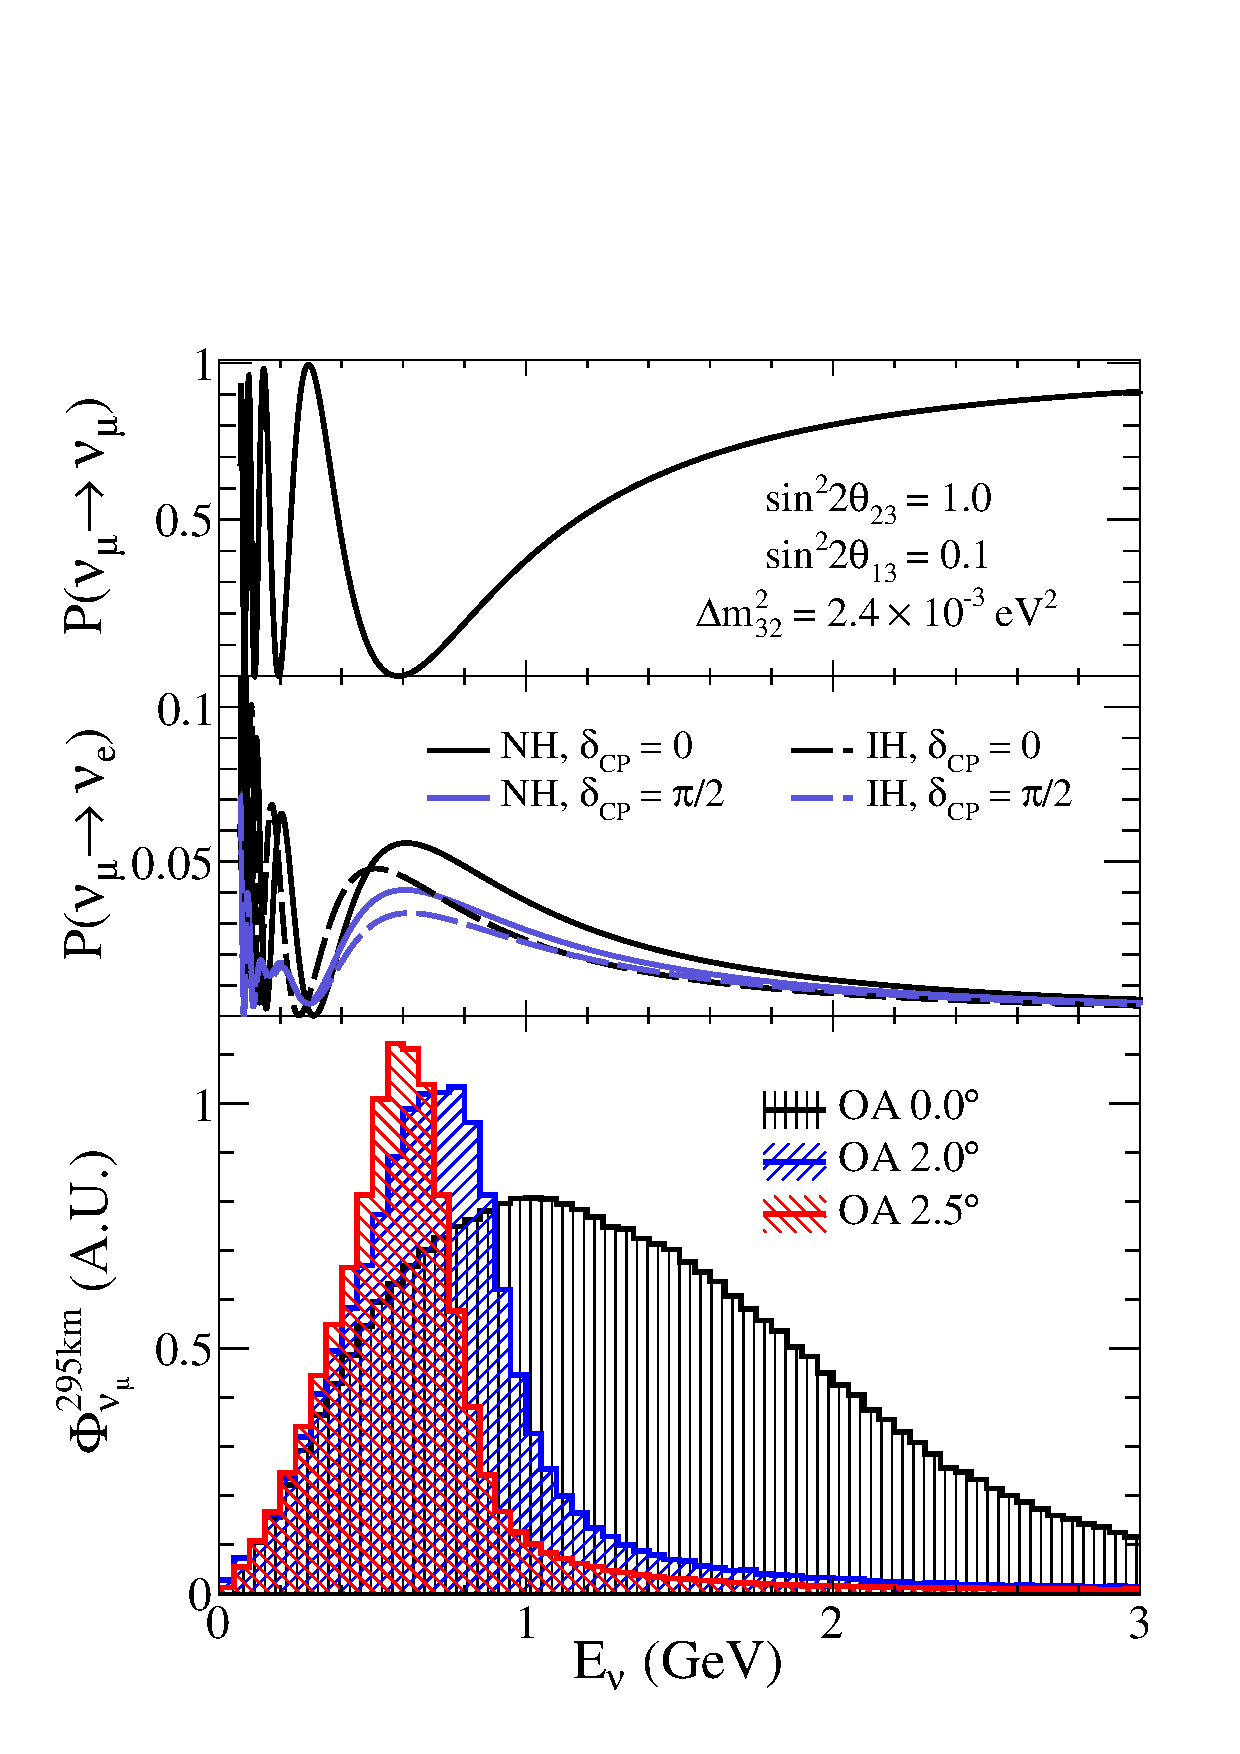
\includegraphics[width=\textwidth, trim={0mm 0mm 0mm 0mm}, clip,page=1]{Figures/Detectors/T2KOffAxisTrick.pdf}
  \end{subfigure}
  \caption{Top panel: T2K muon neutrino disappearance probability as a function of neutrino energy. Middle panel: T2K electron neutrino appearance probability as a function of neutrino energy. Bottom panel: The neutrino flux distribution for three different off-axis angles (Arbitrary units) as a function of neutrino energy.}
  \label{fig:T2KSKExp_T2K_OffAxisTrick}
\end{figure}

\subsection{The Near Detector at \quickmath{280\text{m}}}
\label{subsec:T2KSKExp_T2K_ND280}

Whilst all the near detectors are situated in the same ``pit'' located at \quickmath{280\text{m}} from the beamline, the ``ND280'' detector is the off-axis detector which is situated at the same off-axis angle as the Super-Kamiokande far detector. It has two primary functions; firstly it measures the neutrino flux and secondly it counts the event rates of different types of neutrino interactions. Both of these constrain the flux and cross-section systematics invoked within the model for a more accurate prediction of the expected event rate at the far detector.
%It is designed to observe the unoscillated neutrino flux to measure the beam flux whilst also counting the event rate of the different interaction modes in which a neutrino can interact through. This allows the systematics used within the model to be constrained for a more accurate prediction of the expected event rate at the far detector.

\begin{figure}[h]
  \begin{subfigure}[t]{0.7\textwidth}
    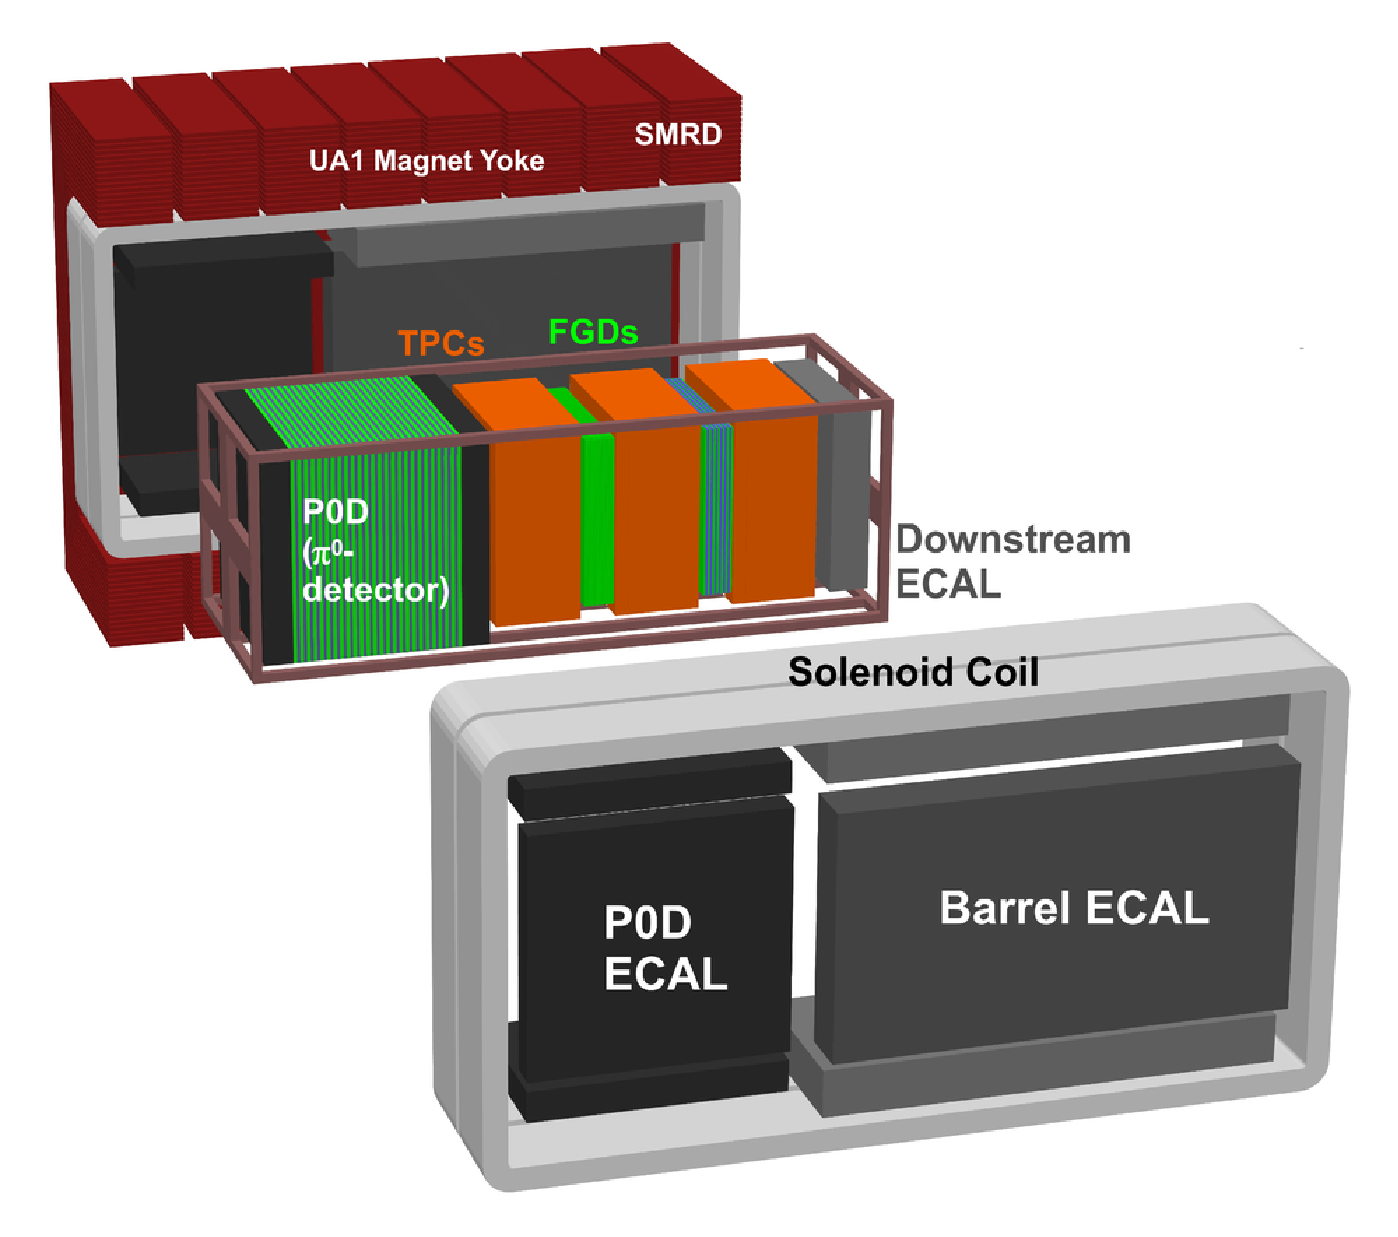
\includegraphics[width=\textwidth, trim={0mm 0mm 0mm 0mm}, clip,page=1]{Figures/Detectors/T2KND280.pdf}
  \end{subfigure}
  \caption{The components of the ND280 detector. The neutrino beam travels from left to right. Taken from \cite{t2k_det}.}
  \label{fig:T2KSKExp_T2K_ND280}
\end{figure}

As illustrated in \autoref{fig:T2KSKExp_T2K_ND280}, the ND280 detector consists of several sub-detectors. The most important part of the detector for this analysis is the tracker region. This is comprised of two time projection chambers (TPCs) sandwiched between three fine grain detectors (FGDs). The FGDs contain both hydrocarbon plastics and water targets for neutrino interactions and provide track reconstruction near the interaction vertex. The emitted charged particles can then propagate into the TPCs which provide particle identification and momentum reconstruction. The FGDs and TPCs are further described in \autoref{subsubsec:T2KSKExp_T2K_FGDs} and \autoref{subsubsec:T2KSKExp_T2K_TPCs} respectively. The electromagnetic calorimeter (ECAL) encapsulates the tracker region alongside the \quickmath{\pi^0} detector (P0D). The ECAL measures the deposited energy from photons emitted from interactions within the FGD. The P0D constrains the cross-section of neutral current interactions which generate neutral pions, which is one of the largest backgrounds in the electron neutrino appearance oscillation channel. The P0D and ECAL detectors are detailed in \autoref{subsubsec:T2KSKExp_T2K_P0D} and \autoref{subsubsec:T2KSKExp_T2K_ECAL} respectively. The entire detector is located within a large yoke magnet which produces a \quickmath{0.2\text{T}} magnetic field. This design of the magnet also includes a scintillating detector called the side muon range detector (SMRD) which is used to track high-angle muons as well as acting as a cosmic veto. The SMRD is described in \autoref{subsubsec:T2KSKExp_T2K_SMRD}.  

\subsubsection{Fine Grained Detectors}
\label{subsubsec:T2KSKExp_T2K_FGDs}

The T2K tracker region is comprised of two fine grained detectors (FGD) and three Time Projection Chambers (TPC). A detailed description of the FGD design, construction, and assembly is found in \cite{Amaudruz2012} and summarised below. The FGDs are the primary target for neutrino interactions with a mass of \quickmath{1.1} tonnes per FGD.
%material which are \quickmath{1.1} tonnes of target material per FDG for the neutrinos to interaction with.
Alongside this, the FGDs are designed to be able to track short-range particles which do not exit the FGD. Typically, short-range particles are low momentum and are observed as tracks that deposit a large amount of energy per unit length. This means the FGD needs good granularity to resolve these particles. The FGDs have the best timing resolution (\quickmath{\sim 3\text{ns}}) of any of the sub-detectors of the ND280 detector. As such, the FGDs are used for time of flight measurements to distinguish forward going positively charged particles from backward going negatively charged particles. Finally, any tracks which pass through multiple sub-detectors are required to be track matched to the FGD.

Both FGDs are made from square scintillator planes of side length \quickmath{186\text{cm}} and width \quickmath{2.02\text{cm}}. Each plane consists of two layers of 192 scintillator bars in an X or Y orientation. A wavelength shifting fiber is threaded through the centre of each bar and is read out by a multi-pixel photon counter (MPPC). FGD1 is the most upstream of the two FGDs and contains 15 planes of carbon plastic scintillator which is a common target in external neutrino scattering data. As the far detector is a pure water target, 7 of the 15 scintillator planes in FGD2 have been replaced with a hybrid water-scintillator target. Due to the complexity of the nucleus, nuclear effects can not be extrapolated between different nuclei. Therefore having the ability to take data on one target which is the same as external data and another target which is the same as the far detector target is beneficial for reliable model parameter estimates.

\begin{figure}[h]
  \begin{subfigure}[t]{0.7\textwidth}
    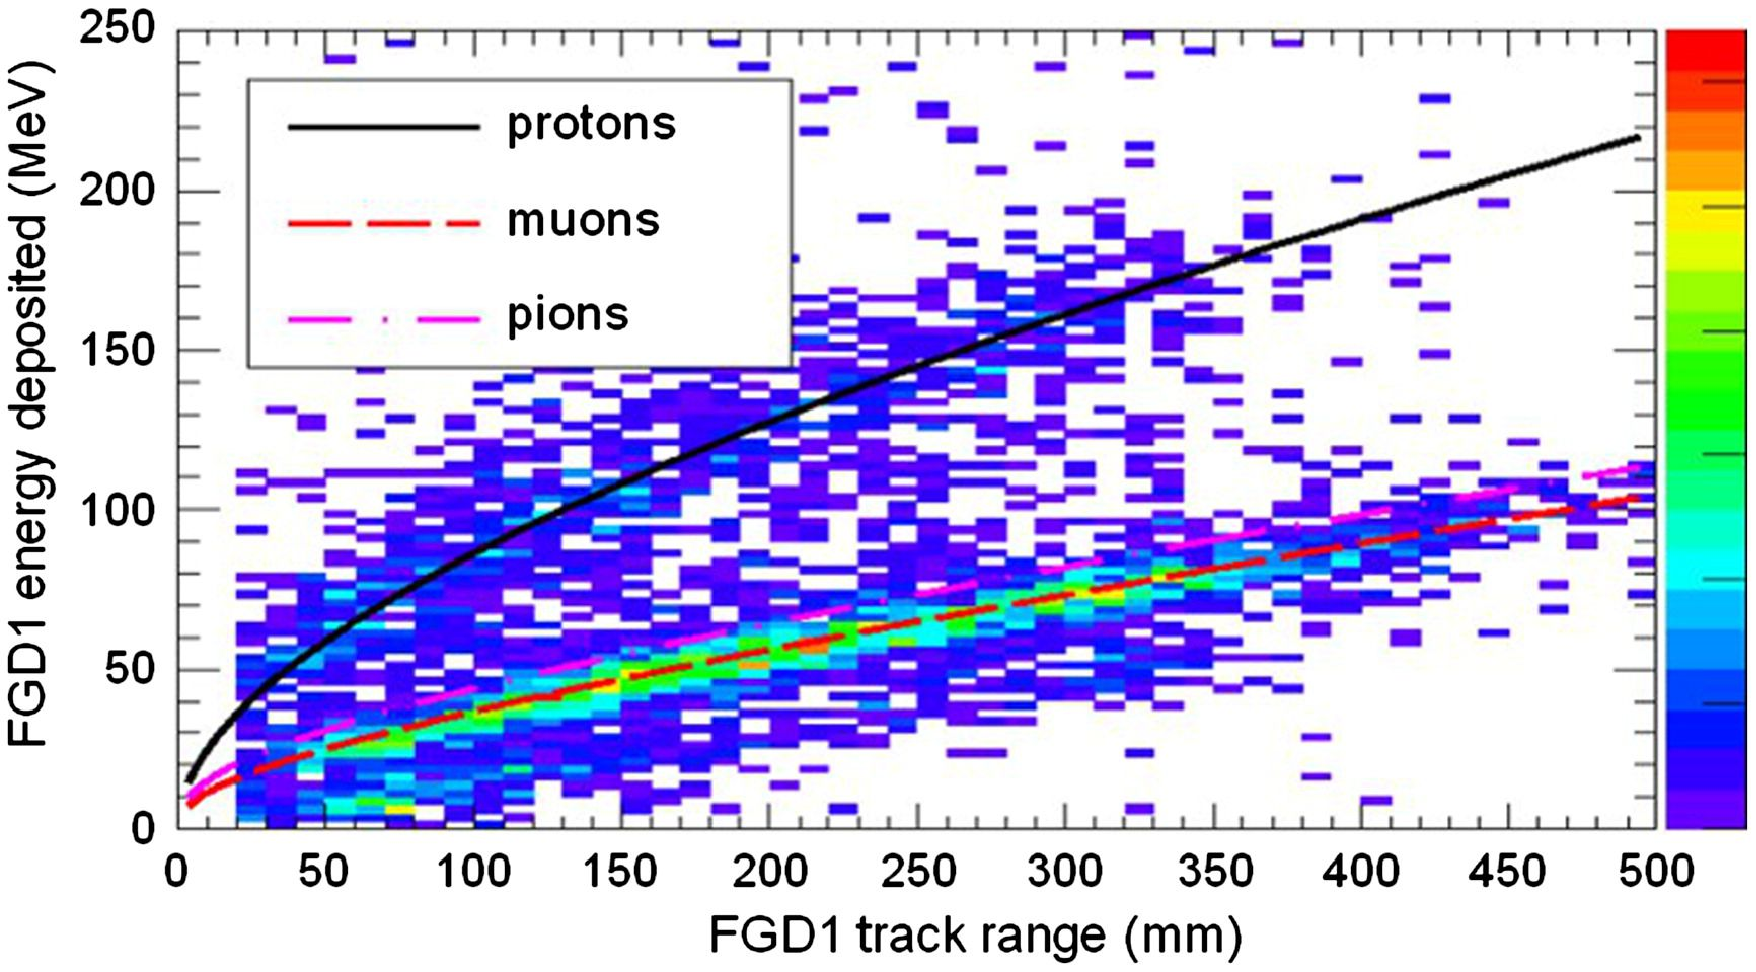
\includegraphics[width=\textwidth, trim={0mm 0mm 0mm 0mm}, clip,page=1]{Figures/Detectors/T2KFGDPID.pdf}
  \end{subfigure}
  \caption{Comparison of data to Monte Carlo prediction of integrated deposited energy as a function of track length for particles that stopped in FGD1. Taken from \cite{Amaudruz2012}.}
  \label{fig:T2KSKExp_T2K_FGDPID}
\end{figure}

The integrated deposited energy is used for particle identification. The FGD can distinguish protons from other charged particles by comparing the integrated deposited energy from data to Monte Carlo prediction as seen in \autoref{fig:T2KSKExp_T2K_FGDPID}.

\subsubsection{Time Projection Chambers}
\label{subsubsec:T2KSKExp_T2K_TPCs}

The majority of particle identification and momentum measurements within ND280 are provided by three Time Projection Chambers (TPCs) \cite{Abgrall2011}. The TPCs are located on either side of the FGDs. They are located inside of the magnetic field meaning the momentum of a charged particle can be determined from the bending of the track.
%They are designed with a momentum resolution of \quickmath{0.2\%} in order not to limit the determination of \delmsqatm at the far detector. Furthermore, to measure the intrinsic \quickmath{\nu_e} contamination of the beam, the resolution of the ionization energy loss is better than \quickmath{10\%} to ensure reliable particle identification.

Each TPC module consists of two gas-tight boxes, as shown in \autoref{fig:T2KSKExp_T2K_TPCDesign}, which are made of non-magnetic material. The outer box is filled with \quickmath{\text{CO}_2} which acts as an electrical insulator between the inner box and the ground. The inner box forms the field cage which produces a uniform electric drift field of \quickmath{\sim 275 \text{V/cm}} and is filled with an argon gas mixture. Charged particles moving through this gas mixture ionize the gas and the ionised charge is drifted towards micromegas detectors which measure the ionization charge. The time and position information in the readout allows a three-dimensional image of the neutrino interaction.

\begin{figure}[h]
  \begin{subfigure}[t]{0.55\textwidth}
    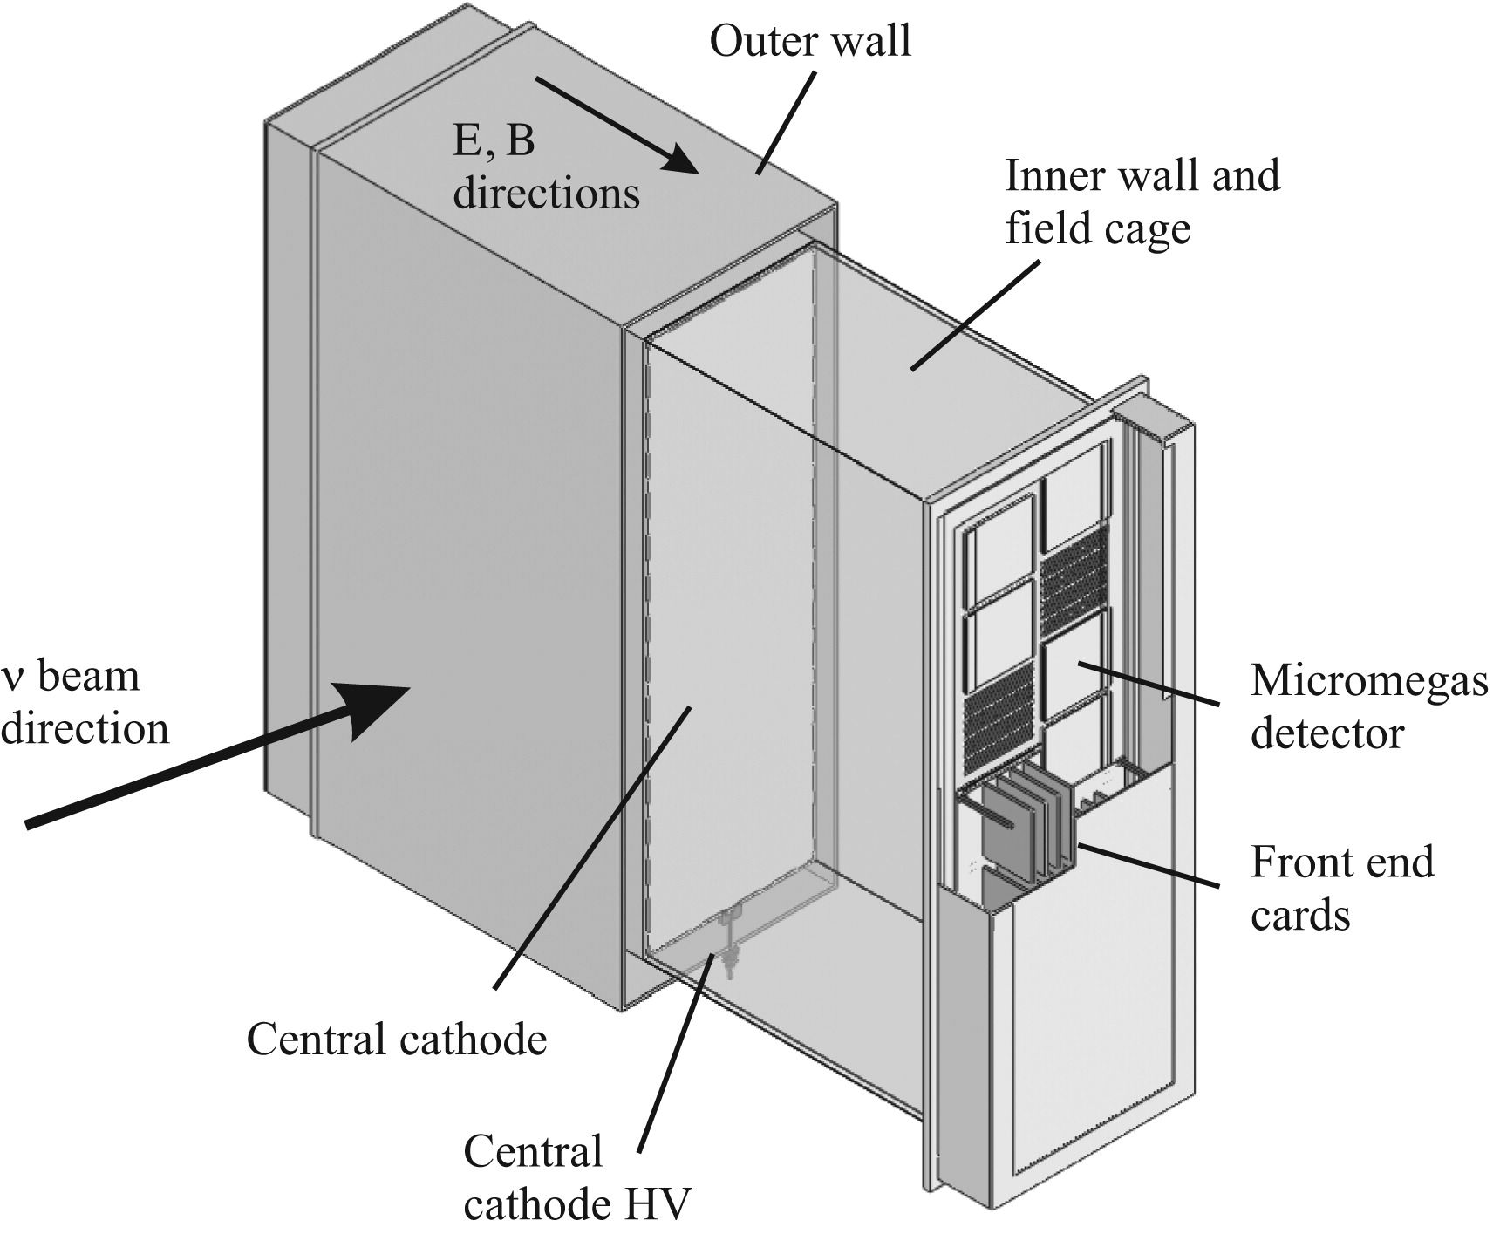
\includegraphics[width=\textwidth, trim={0mm 0mm 0mm 0mm}, clip,page=1]{Figures/Detectors/T2KTPCDesign.pdf}
  \end{subfigure}
  \caption{Schematic design of a Time Projection Chamber detector. Taken from \cite{Abgrall2011}.}
  \label{fig:T2KSKExp_T2K_TPCDesign}
\end{figure}

The particle identification of tracks that pass through the TPCs is performed using dE/dx measurements. \autoref{fig:T2KSKExp_T2K_TPC_dEdx} illustrates the data to Monte Carlo distributions of the energy lost by a charged particle passing through the TPC as a function of the reconstructed particle momentum. The resolution is \quickmath{7.8 \pm 0.2\%} meaning that electrons and muons can be distinguished. This allows reliable measurements of the intrinsic \quickmath{\nu_e} component of the beam.

\begin{figure}[h]
  \begin{subfigure}[t]{0.48\textwidth}
    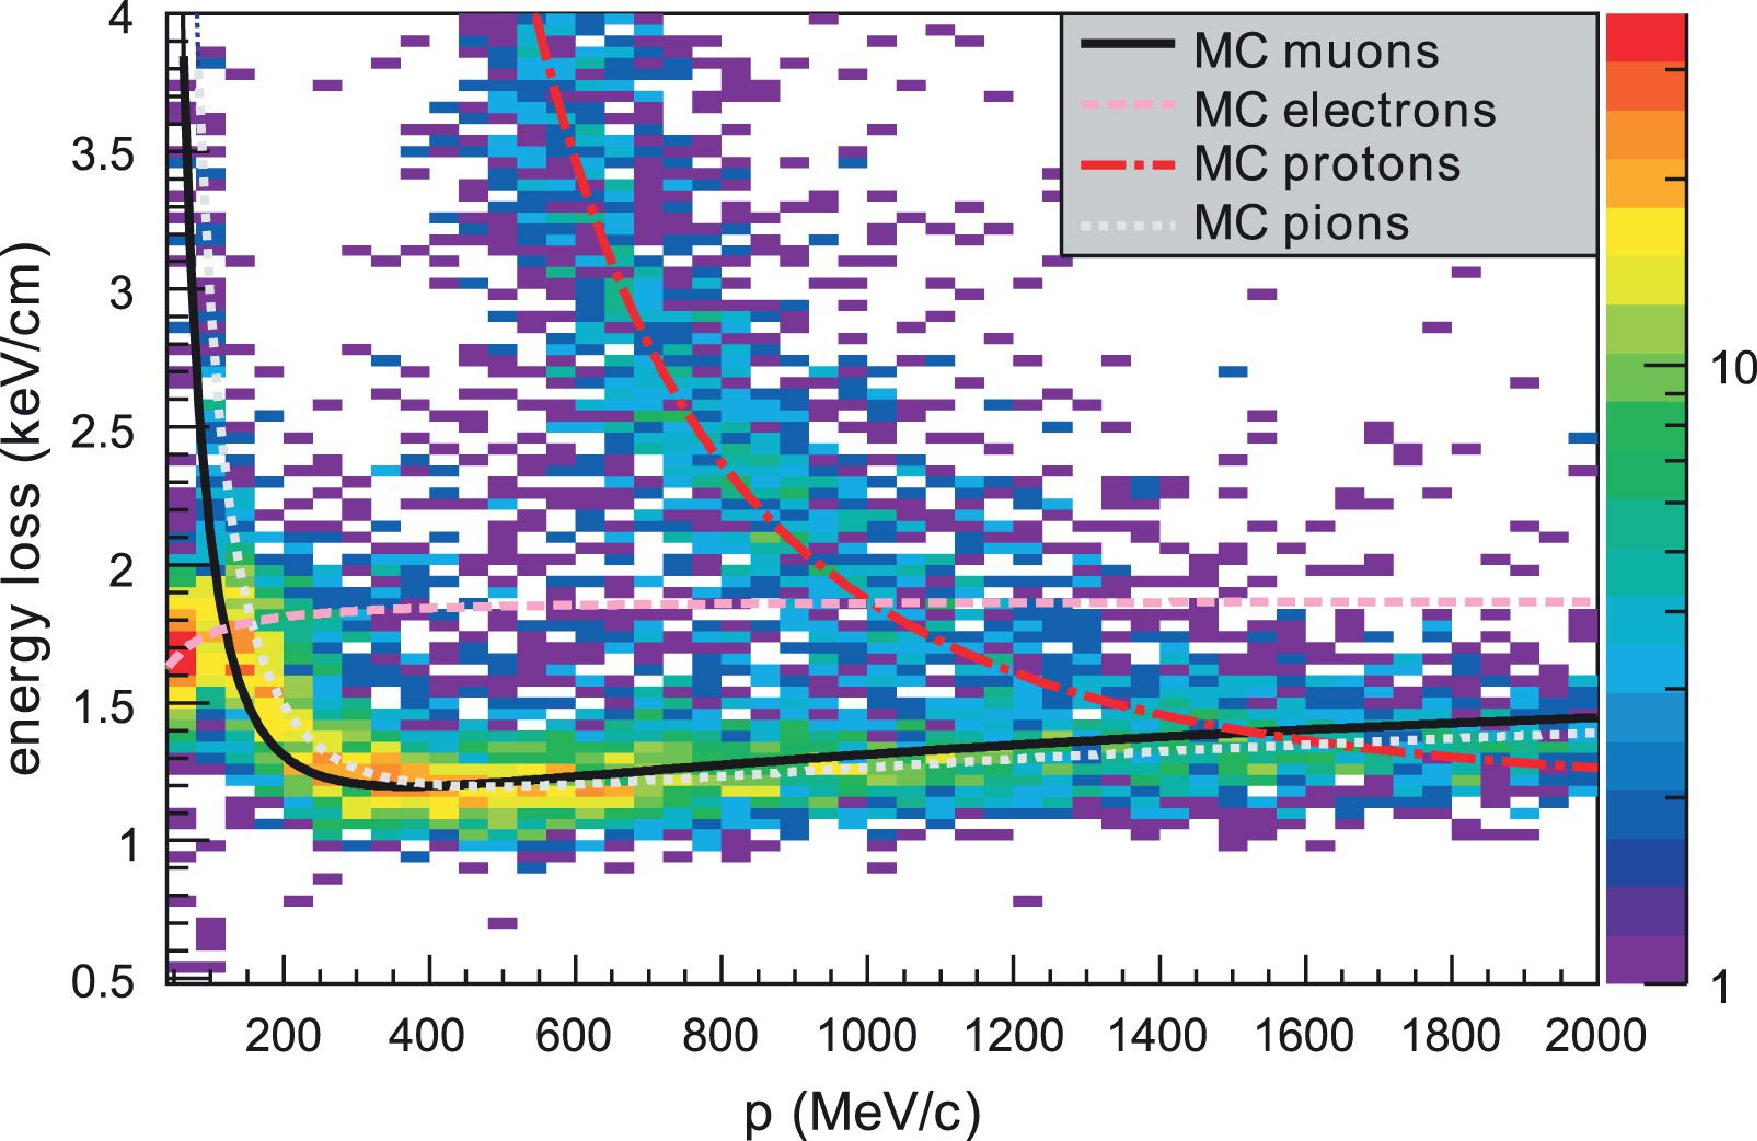
\includegraphics[width=\textwidth, trim={0mm 0mm 0mm 0mm}, clip,page=1]{Figures/Detectors/T2K_TPCdEdx_Positive.pdf}
    \subcaption{Positively charged particles}
  \end{subfigure}%
  \begin{subfigure}[t]{0.48\textwidth}
    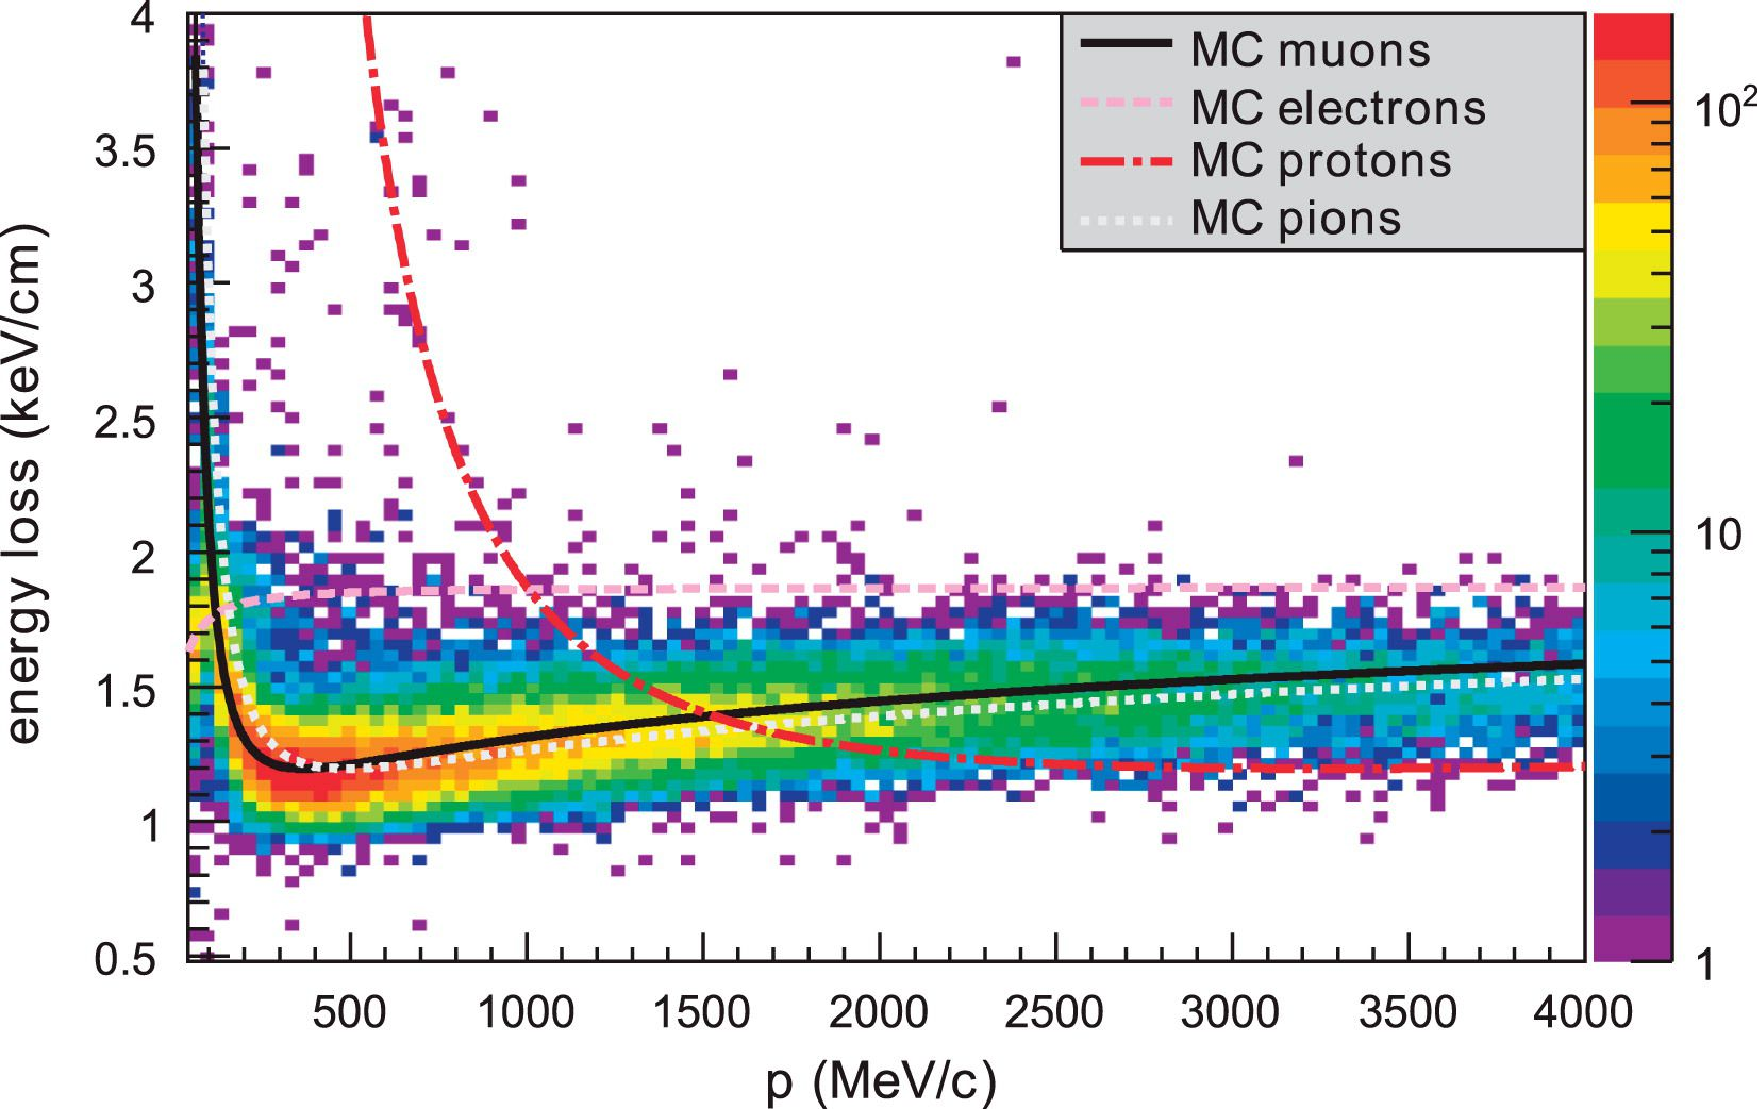
\includegraphics[width=\textwidth, trim={0mm 0mm 0mm 0mm}, clip,page=1]{Figures/Detectors/T2K_TPCdEdx_Negative.pdf}
    \subcaption{Negatively charged particles}
  \end{subfigure}
  \caption{The distribution of energy loss as a function of reconstructed momentum for charged particles passing through the TPC, comparing data to Monte Carlo prediction. Taken from \cite{Abgrall2011}.}
  \label{fig:T2KSKExp_T2K_TPC_dEdx}
\end{figure}

\subsubsection{\quickmath{\pi^0} Detector}
\label{subsubsec:T2KSKExp_T2K_P0D}

If one of the \quickmath{\gamma}-rays from a \quickmath{\pi^0 \rightarrow 2\gamma} decay is missed at the far detector, the reconstruction will determine that event to be a charge current \quickmath{\nu_{e}}-like event. This is one of the main backgrounds hindering the electron neutrino appearance searches. The \quickmath{\pi^0} detector (P0D) measures the cross-section of the neutral current induced neutral pion production on a water target to constrain this background.

The P0D is a cube of approximately \quickmath{2.5\text{m}} length consisting of layers of scintillating bars, brass and lead sheets, and water bags as illustrated in \autoref{fig:T2KSKExp_T2K_P0DDesign}. Two electromagnetic calorimeters are positioned at the most upstream and most downstream position in the sub-detector and the water target is situated in between them. The scintillator layers are built from two triangular bars orientated in opposite directions to form a rectangular layer. Each triangular scintillator bar is threaded with optical fiber which is read out by MPPCs. The high-Z brass and lead regions produce electron showers from the photons emitted in \quickmath{\pi^0} decay.

\begin{figure}[h]
  \begin{subfigure}[t]{0.55\textwidth}
    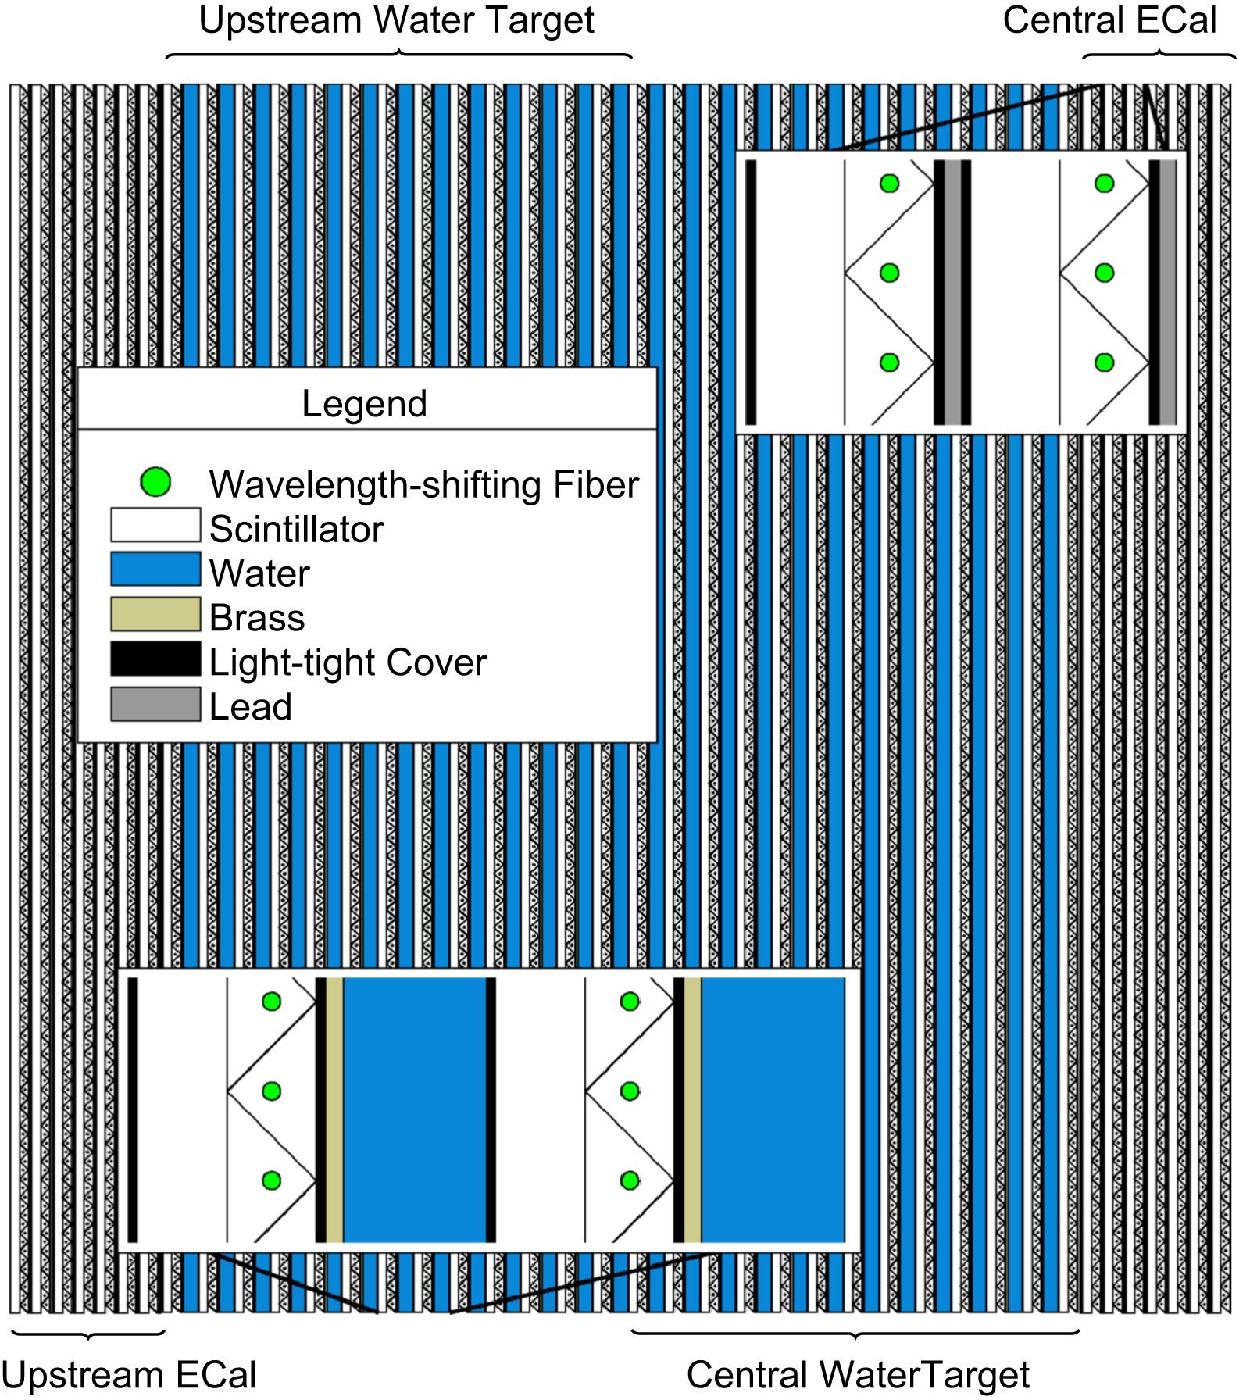
\includegraphics[width=\textwidth, trim={0mm 0mm 0mm 0mm}, clip,page=1]{Figures/Detectors/T2KP0DDesign.pdf}
  \end{subfigure}
  \caption{A schematic of the P0D side-view. Taken from \cite{Assylbekov2012}.}
  \label{fig:T2KSKExp_T2K_P0DDesign}
\end{figure}

The sub-detector can generate measurements of NC\quickmath{1\pi^0} cross-sections on a water target by measuring the event rate both with and without the water target, with the cross-section on a water target being determined as the difference. The total active mass is \quickmath{16.1} tonnes when filled with water and \quickmath{13.3} tonnes when empty.

\subsubsection{Electromagnetic Calorimeter}
\label{subsubsec:T2KSKExp_T2K_ECAL}

The electromagnetic calorimeter \cite{Allan_2013} (ECal) encapsulates the P0D and tracking sub-detectors. Its primary purpose is to aid \quickmath{\pi^0} reconstruction from any interaction in the tracker. To do this, it measures the energy and direction of photon showers from \quickmath{\pi^0 \rightarrow 2\gamma} decay. It can also distinguish pion and muon tracks depending on the shape of the photon shower deposited.

The ECal is comprised of three sections; the P0D ECal which surrounds the P0D, the barrel ECal which encompasses the tracking region, and the downstream ECal which is situated downstream of the tracker region. The barrel and downstream ECals are tracking calorimeters that focus on electromagnetic showers from high-angle particles emitted from the tracking sub-detectors. Particularly in  the TPC, high-angle tracks (those which travel perpendicularly to the beam-axis) can travel along a single scintillator bar resulting in very few hits. The width of the barrel and downstream ECal corresponds to \quickmath{\sim 11} electron radiation lengths to ensure a significant amount of the \quickmath{\pi^{0}} energy is contained. As the P0D has its own calorimetry which reconstructs showers, the P0D ECal determines the energy which escapes the P0D.

Each ECal is constructed of multiple layers of scintillating bars sandwiched between lead sheets. The scintillating bars are threaded with optical fiber and read out by MPPCs. Each sequential layer of the scintillator is orientated perpendicular to the previous which allows a three dimensional event reconstruction. The target mass of the P0D ECal, barrel ECal, and downstream ECal are \quickmath{1.50}, \quickmath{4.80} and \quickmath{6.62} tonnes respectively.

\subsubsection{Side Muon Range Detector}
\label{subsubsec:T2KSKExp_T2K_SMRD}

As illustrated in \autoref{fig:T2KSKExp_T2K_ND280}, the ECal, FGDs, P0D, and TPCs are enclosed within the UA1 magnet. Originally designed for the NOMAD \cite{Vannucci2014} experiment and reconditioned for use in the T2K experiment \cite{cerncourier_2022}, the UA1 magnet provides a uniform horizontal magnetic field of 0.2\text{T} with an uncertainty of \quickmath{2\times10^{-4}\text{T}}.

Built into the UA1 magnet, the side muon range detector (SMRD)\cite{Aoki2013} monitors high-energy muons which leave the tracking region and permeate through the ECal. It additionally acts as a cosmic muon veto and trigger. 

\subsection{The Interactive Neutrino GRID}
\label{subsec:T2KSKExp_T2K_INGRID}

The Interactive Neutrino GRID (INGRID) detector is situated within the same ``pit'' as the other near detectors. It is aligned with the beam in the ``on-axis'' position and measures the beam direction, spread, and intensity. The detector was originally designed with 16 identical modules \cite{t2k_det} (two modules have since been decommissioned) and a ``proton'' module. The design of the detector is cross-shaped with length and height \quickmath{10\text{m} \times 10\text{m}} as illustrated in \autoref{fig:T2KSKExp_T2K_INGRID}.

Each module is composed of iron sheets interlaced with eleven tracking scintillator planes for a total target mass of \quickmath{7.1} tonnes per module. The scintillator design is an X-Y pattern of 24 bars in both orientations, where each bar contains wave-length shifting fibers which are connected to multi-pixel photon counters (MPPCs). Each module is encapsulated inside veto planes to aid the rejection of charged particles entering the module.

The proton module is different from the other modules in that it consists of entirely scintillator planes with no iron target. The scintillator bars are also smaller than those used in the other modules to increase the granularity of the detector and improve tracking capabilities. The module sits in the centre of the beamline and is designed to give precise measurements of quasi-elastic charged current interactions to evaluate the performance of the Monte Carlo simulation of the beamline. 

\begin{figure}[h]
  \begin{subfigure}[t]{0.45\textwidth}
    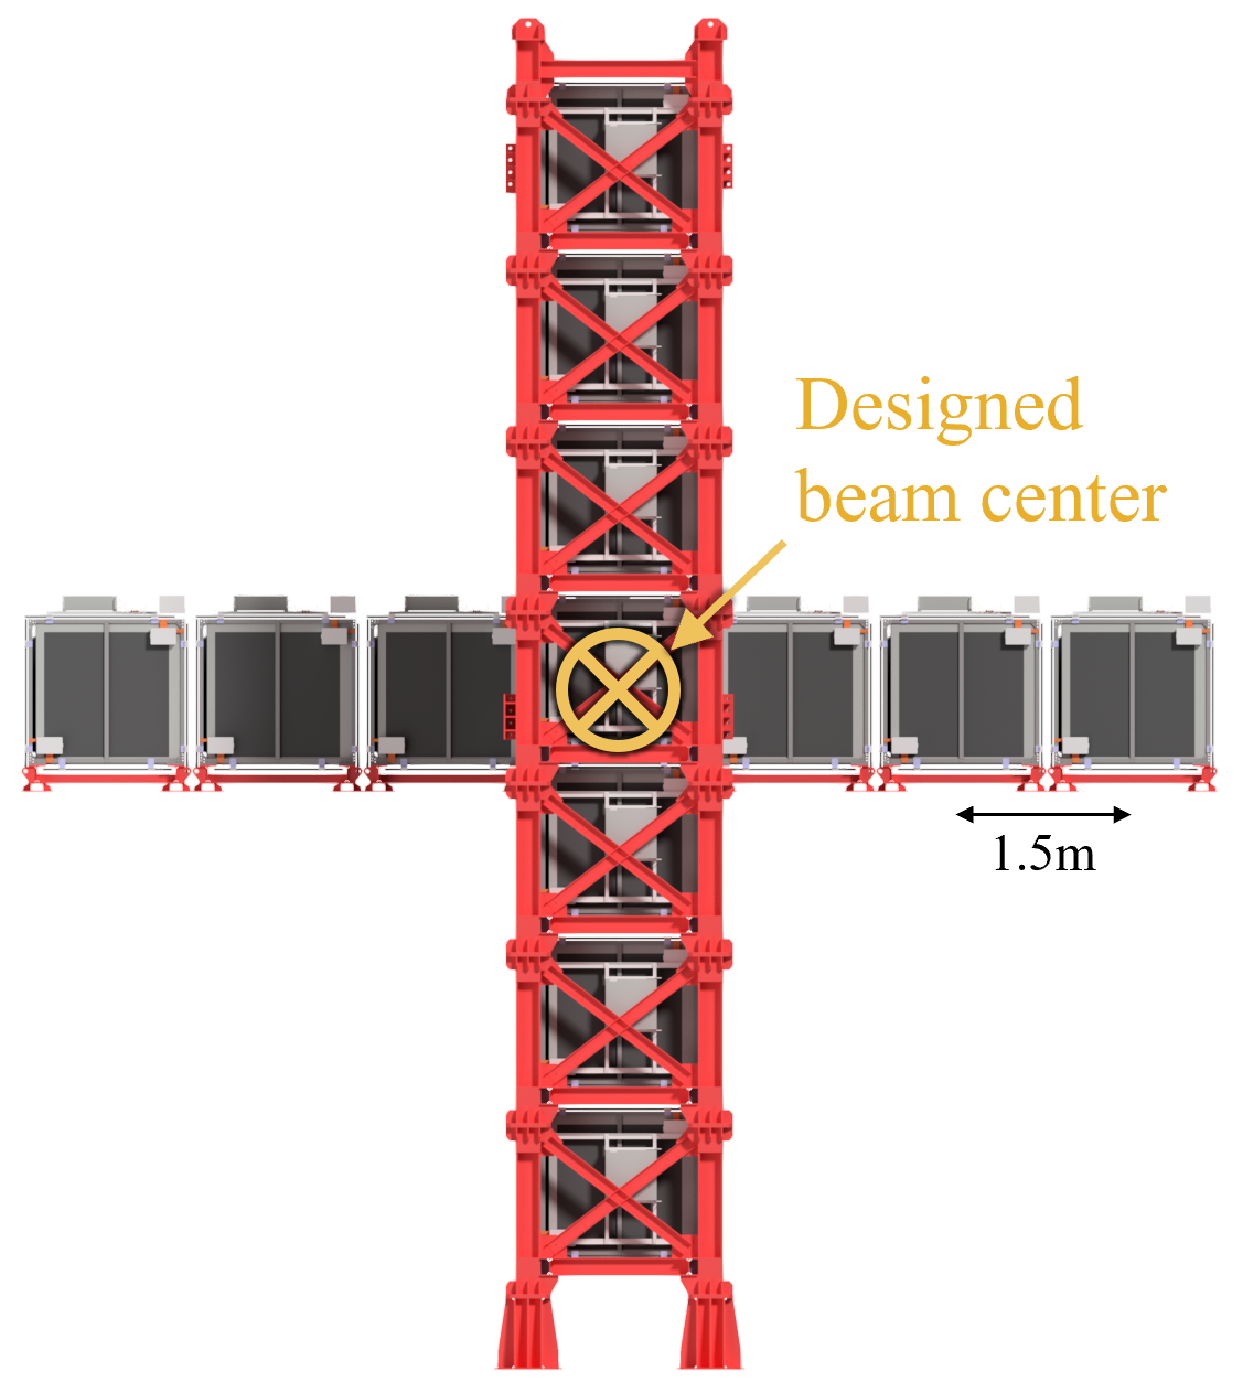
\includegraphics[width=\textwidth, trim={0mm 0mm 0mm 0mm}, clip,page=1]{Figures/Detectors/T2KINGRIDDiagram.pdf}
  \end{subfigure}%
  \begin{subfigure}[t]{0.55\textwidth}
    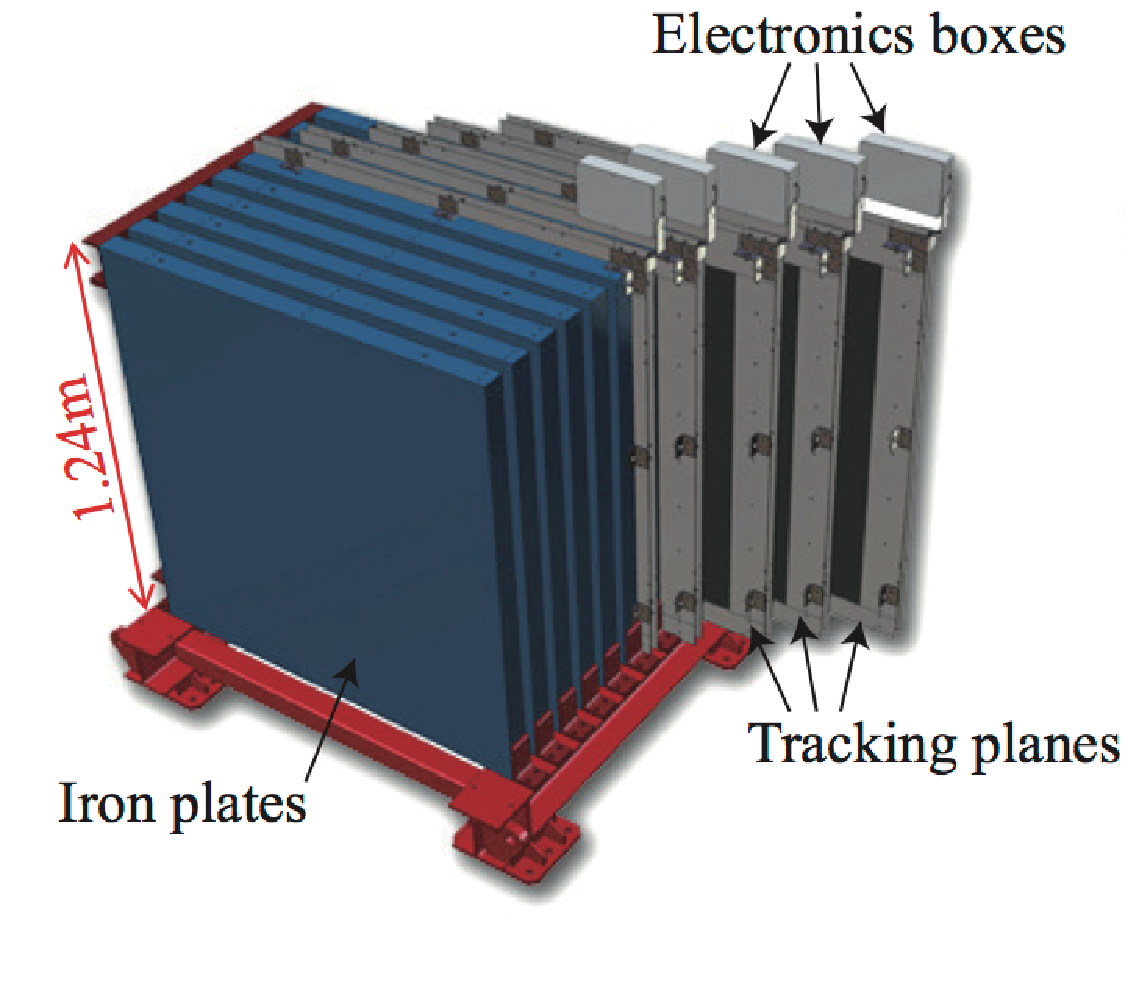
\includegraphics[width=\textwidth, trim={0mm 0mm 0mm 0mm}, clip,page=1]{Figures/Detectors/T2KINGRIDModule.pdf}
  \end{subfigure}%
  \caption{Left panel: The Interactive Neutrino GRID on-axis Detector. 14 modules are arranged in a cross-shape configuration, with the centre modules being directly aligned with the on-axis beam. Right panel: The layout of a single module of the INGRID detector. Both figures are recreated from \cite{t2k_det}.}
  \label{fig:T2KSKExp_T2K_INGRID}
\end{figure}

The INGRID detector can measure the beam direction to an uncertainty of \quickmath{0.4\text{mrad}} and the beam centre within a resolution of \quickmath{10 \text{cm}} \cite{t2k_det}. The beam direction in both the vertical and horizontal directions is discussed in \cite{Suzuki_2015} and it is found to be in good agreement with the MUMON monitor described in \autoref{subsec:T2KSKExp_T2K_NeutrinoBeam}.


  \chapter{Bayesian Statistics and Markov Chain Monte Carlo Techniques}
\label{chap:MarkovChainMonteCarlo}
This thesis presents a Bayesian oscillation analysis. To extract the oscillation parameters, a Markov Chain Monte Carlo (MCMC) method is used. This chapter explains the theory of how parameter estimates can be determined using this technique and condenses the material found in the literature \cite{mcmc_handbook, mcmc_practice, thesis_clarence, thesis_kirsty}.

The oscillation parameter determination presented here is built upon a simultaneous fit to neutrino beam data in the near detector, beam data at SK, and atmospheric data at SK. In total, there are four oscillation parameters of interest (\quickmath{\sin^{2}(\theta_{23})}, \quickmath{\sin^{2}(\theta_{13})}, \quickmath{\Delta m^{2}_{32}}, and \quickmath{\delta_{CP}}), two oscillation parameters to which this study will not be sensitive (\quickmath{\sin^{2}(\theta_{12})}, \quickmath{\Delta m^{2}_{21}}) and  many nuisance parameters that control the systematic uncertainty models.
%The systematic uncertainties can be grouped into categories depending on how they are defined: $574$ bin-normalisations due to the near detector response, $45$ bin-normalisations to describe the far detector response to neutrino beam events, $27$ parameters to describe the detector response to atmospheric neutrino events, $100$ to model the bin-normalisation due to beam flux uncertainties, $18$ which model the atmospheric flux uncertainties, and $87$ to describe the correlated cross-section model. An alternative parameterisation, where the far detector response is correlated between the beam and atmospheric samples, replaces the bin-normalisation parameters with $224$ shift and smear systematics. Section Link to Systematics Chapter describes the systematic model in more depth.

This analysis uses a Monte Carlo technique to generate a multi-dimensional probability distribution across all of the model parameters used in the fit. To determine an estimate for each parameter, this multi-dimensional object is integrated over all other parameters. This process is called Marginalisation and is described in \autoref{sec:MarkovChainMonteCarlo_Marginalisation}. Monte Carlo techniques approximate the probability distribution of each parameter within the limit of generating infinite samples. As ever, generating a large number of samples is time and resource-dependent. Therefore, an MCMC technique is utilised within this analysis to reduce the required number of steps to sufficiently sample the parameter space. This technique is described in further detail in \autoref{sec:MarkovChainMonteCarlo_MarkovChainMC}.

\finish{Introduce MaCh3 and say what I did on it}

\section{Bayesian Statistics}
\label{sec:MarkovChainMonteCarlo_BayesianStatistics}

Bayesian inference treats observable data, \quickmath{D}, and model parameters, \quickmath{\vec{\theta}}, on equal footing such that a probability model of both data and parameters is required. This is the joint probability distribution \quickmath{P(D, \vec{\theta})} and can be described by the prior distribution for model parameters \quickmath{P(\vec{\theta})} and the likelihood of the data given the model parameters \quickmath{P(D|\vec{\theta})},

\begin{equation}
  P(D,\vec{\theta}) = P(D|\vec{\theta})P(\vec{\theta}).
\end{equation}

The prior distribution, \quickmath{P(\vec{\theta})}, describes all previous knowledge about the parameters within the model. For example, if the risk of developing health problems is known to increase with age, the prior distribution would describe the increase. For the purpose of this analysis, the prior distribution is typically the best-fit values taken from external data measurements with a Gaussian uncertainty. The prior distribution can also contain correlations between model parameters. In an analysis using Monte Carlo techniques, the likelihood of measuring some data assuming some set of model parameters is calculated by comparing the Monte Carlo prediction generated at that particular set of model parameters to the data.

It is parameter estimation that is important for this analysis and as such, we apply Bayes' theorem \cite{Bayes:1764vd} to calculate the probability for each parameter to have a certain value given the observed data, \quickmath{P(\vec{\theta}|D)}, which is known as the posterior distribution (often termed the posterior). This can be expressed as

\begin{equation}
  \label{eq:MarkovChainMonteCarlo_PosteriorDistribution}
  P(\vec{\theta}|D) = \frac{ P(D|\vec{\theta}) P(\vec{\theta}) }{\int P(D|\vec{\theta}) P(\vec{\theta}) d\vec{\theta}}.
\end{equation}

The denominator in \autoref{eq:MarkovChainMonteCarlo_PosteriorDistribution} is the integral of the joint probability distribution over all values of all parameters used within the fit. For brevity, we say that the posterior distribution is

\begin{equation}
  \label{eq:MarkovChainMonteCarlo_PosteriorDistributionReduced}
  P(\vec{\theta}|D) \propto P(D|\vec{\theta}) P(\vec{\theta}).
\end{equation}

%In \autoref{sec:MarkovChainMonteCarlo_Marginalisation}, we see that for the cases used within this analysis, it is reasonable to know the posterior to some normalisation constant.
For the purposes of this analysis, it is acceptable to neglect the normalisation term and focus on this proportional relationship.

\subsection{Application of Prior Knowledge}
\label{sec:MarkovChainMonteCarlo_Priors}

The posterior distribution is proportional to the prior uncertainty applied to each parameter, as illustrated by \autoref{eq:MarkovChainMonteCarlo_PosteriorDistributionReduced}. This means that it is possible to change the prior after the posterior distribution has been determined. The prior uncertainty of a particular parameter can be `divided' out of the posterior distribution and the resulting distribution can be reweighted using the new prior uncertainty that is to be applied. The methodology and implementation of changing the prior follows that described in \cite{thesis_artur}. 

An example implementation that is useful for this analysis is the application of the ``reactor constraint''. As discussed in \autoref{sec:Theory_Summary}, an external constraint on \quickmath{\sin^{2}(\theta_{13})} is determined from measurements taken from reactor experiments. However, the sensitivities from just using the T2K and SK samples is equally as important. Without this technique, two fits would have to be run, doubling the required resources. Therefore, the key benefit for this analysis is the fact that only a single `fit' has to be performed and can be used to build the two posterior distributions of the with and without reactor constraint applied.

\section{Monte Carlo Simulation}
\label{sec:MarkovChainMonteCarlo_MonteCarloSimulation}
Monte Carlo techniques are used to numerically solve a complex problem that does not necessarily have an analytical solution. These techniques rely on building a large ensemble of samples from an unknown distribution and then using the ensemble to approximate the properties of the distribution.

An example that uses Monte Carlo techniques is to calculate the area underneath a curve. For example, take the problem of calculating the area under a straight line with gradient \quickmath{M = 0.4} and intercept \quickmath{C = 1.0}. Analytically, one can calculate the area under the line is equal to 30 units for \quickmath{0 \leq x \leq 10}. Using Monte Carlo techniques, one can calculate the area under this line by throwing many random values for the \quickmath{x} and \quickmath{y} components of each sample and then calculating whether that point falls below the line. The area can then be calculated by the ratio of points below the line to the total number of samples thrown multiplied by the total area in which samples were scattered. The study is shown in \autoref{fig:MCMC_MCTechnique} highlights this technique and finds the area under the curve to be \quickmath{29.9} compared to an analytical solution of \quickmath{30.0}. The deviation of the numerical to analytical solution can be attributed to the number of samples used in the study. The accuracy of the approximation in which the properties of the Monte Carlo samples replicate those of the desired distribution is dependent on the number of samples used. Replicating this study with a differing number of Monte Carlo samples used in each study (As shown in \autoref{fig:MCMC_MCTechniqueNThrowsStudy}) highlights how the Monte Carlo techniques are only accurate within the limit of a high number of samples.

Whilst the above example has an analytical solution, these techniques are just as applicable to complex solutions. Clearly,  any numerical solution is only as useful as its efficiency. As discussed, the accuracy of the Monte Carlo technique is dependent upon the number of samples generated to approximate the properties of the distribution. Furthermore, if the positions at which the samples are evaluated are not `cleverly' picked, the efficiency of the Monte Carlo technique significantly drops. Given the example in \autoref{fig:MCMC_MCTechnique}, if the region in which the samples are scattered significantly extends passed the region of interest, many calculations will be calculated but do not add to the ability of the Monte Carlo technique to achieve the correct result. For instance, any sample evaluated at a \quickmath{y \geq 5} could be removed without affecting the final result. This does bring in an aspect of the `chicken and egg' problem in that to achieve efficient sampling, one needs to know the distribution beforehand.

\begin{figure}[h]
  \begin{subfigure}[t]{0.80\textwidth}
    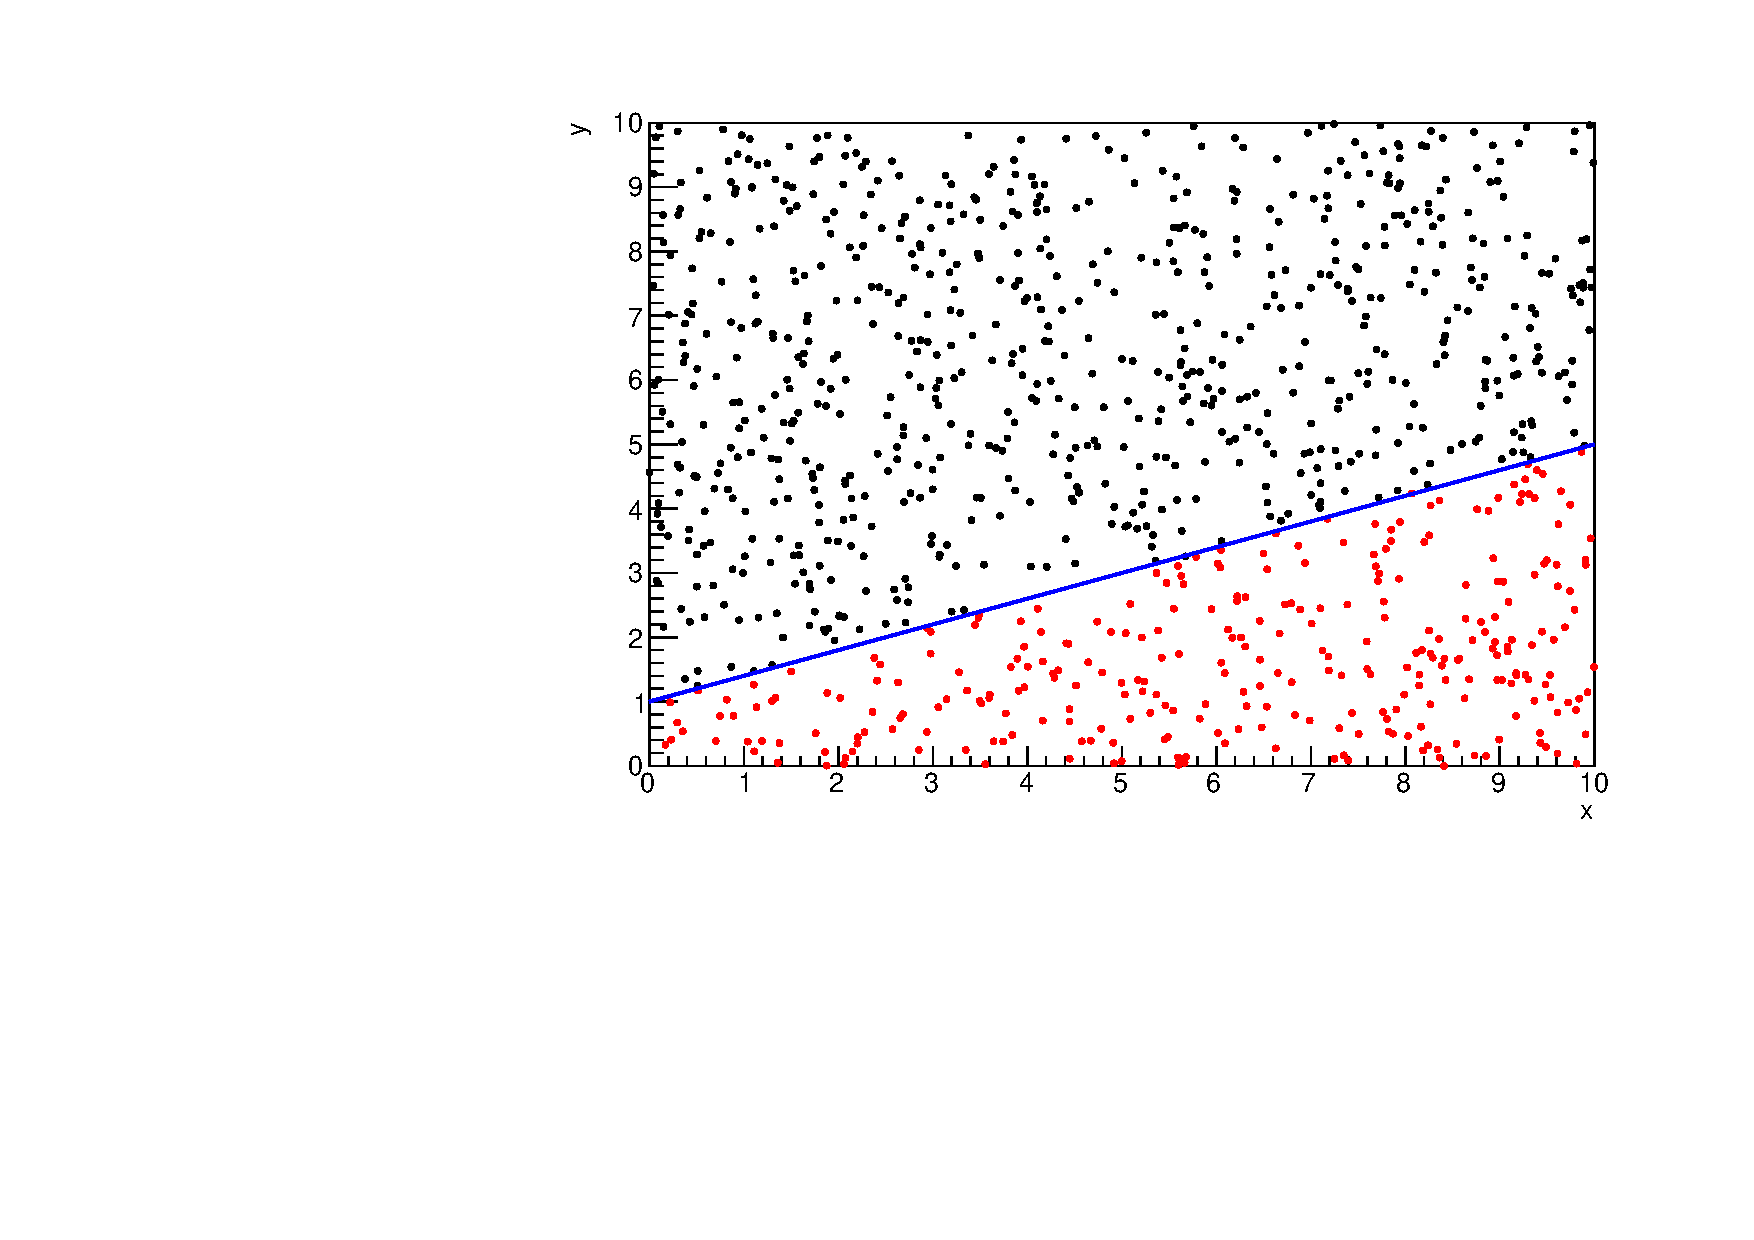
\includegraphics[width=\textwidth, trim={0mm 0mm 0mm 0mm}, clip,page=1]{Figures/MCMC/MCTechnique.pdf}
  \end{subfigure}
  \caption{Example of using Monte Carlo techniques to find the area under the blue line. The gradient and intercept of the line are \quickmath{0.4} and \quickmath{1.0} respectively. The area found to be under the curve using one thousand samples is \quickmath{29.9} units.}
  \label{fig:MCMC_MCTechnique}
\end{figure}

\begin{figure}[h]
  \begin{subfigure}[t]{0.80\textwidth}
    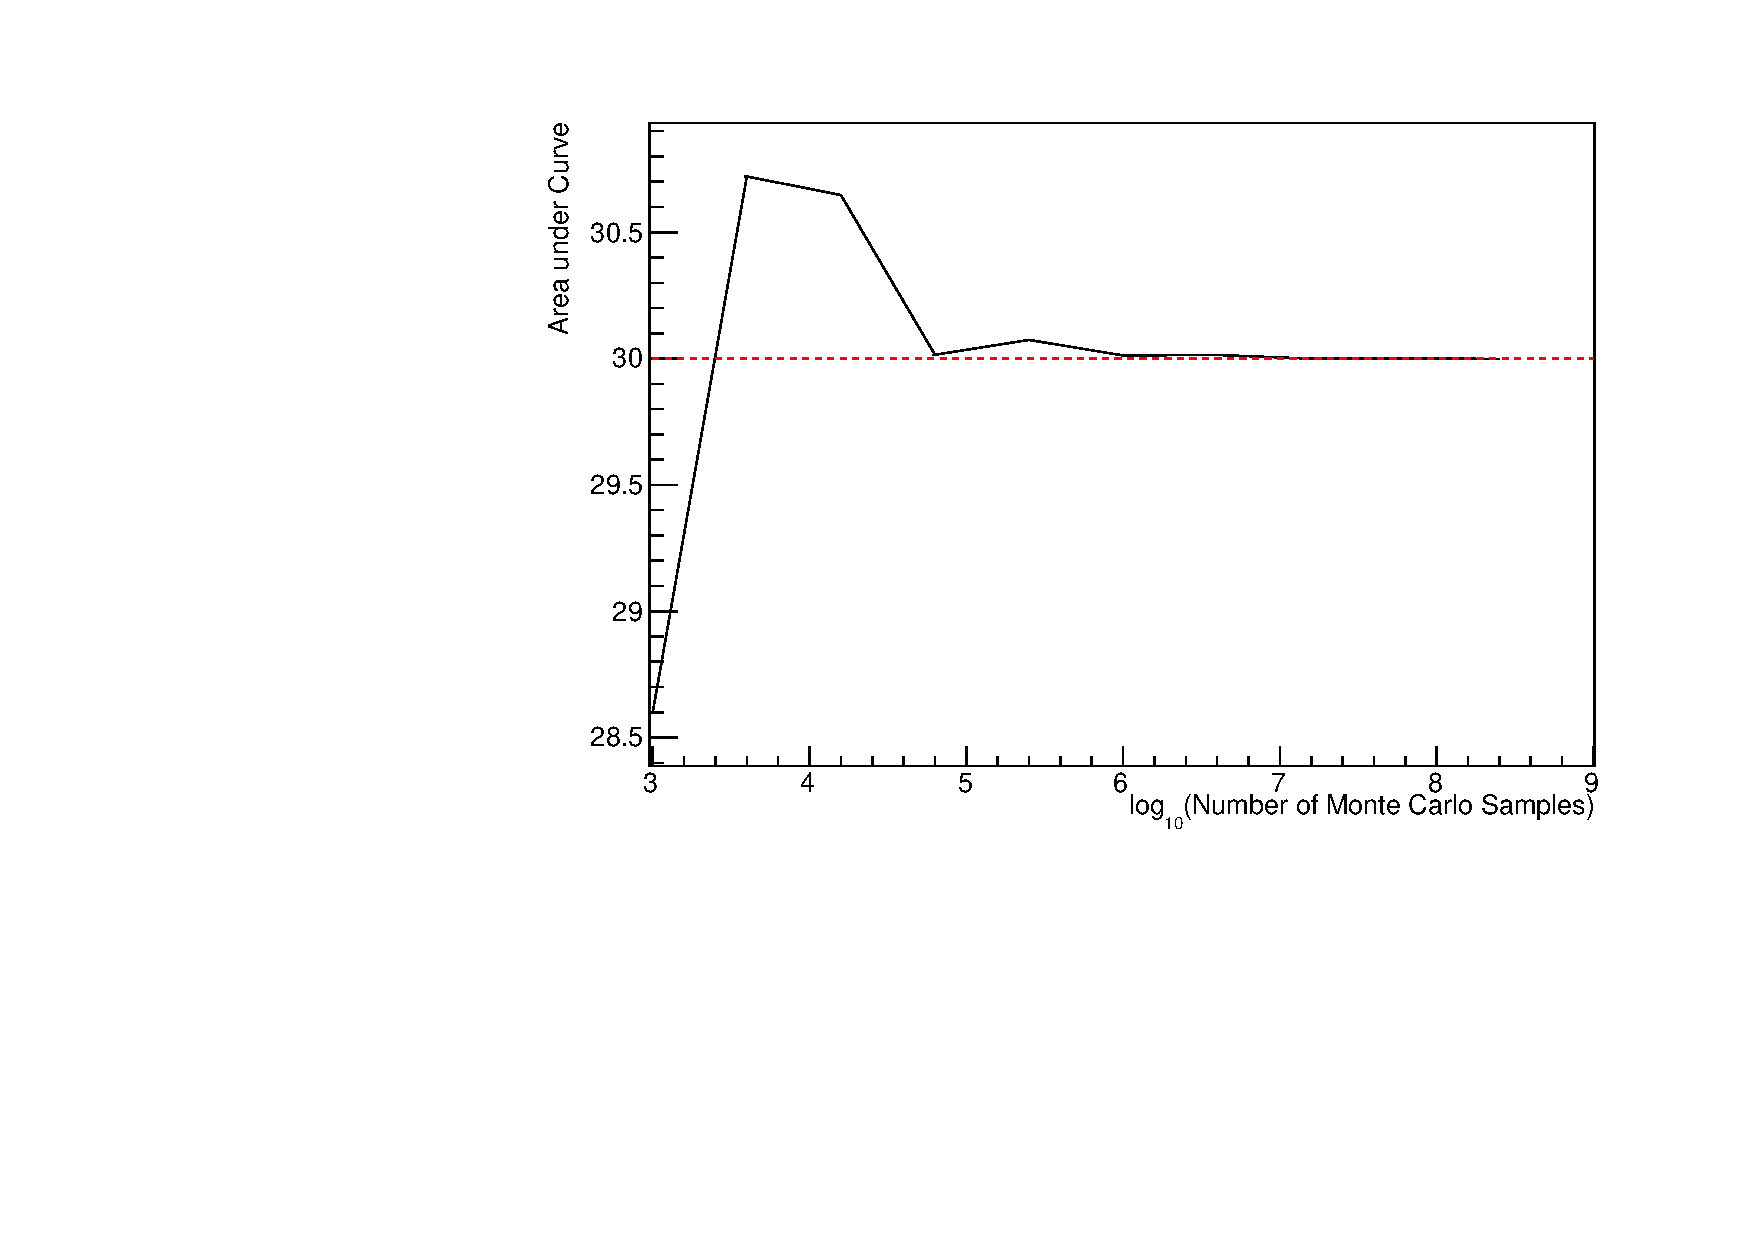
\includegraphics[width=\textwidth, trim={0mm 0mm 0mm 0mm}, clip,page=1]{Figures/MCMC/MCTechnique_NThrowsStudy.pdf}
  \end{subfigure}
  \caption{The area under a line of gradient \quickmath{0.4} and intercept \quickmath{1.0} for the range \quickmath{0 \leq x \leq 10} as calculated using Monte Carlo techniques as a function of the number of samples used in each repetition. The analytical solution to the area is 30 units as given by the red line.}
  \label{fig:MCMC_MCTechniqueNThrowsStudy}
\end{figure}

\subsection{Markov Chain Monte Carlo}
\label{sec:MarkovChainMonteCarlo_MarkovChainMC}
This analysis utilises a multi-dimensional probability distribution, with some dimensions being significantly more constrained than others. These constraints can be from prior knowledge of parameter distributions from external data or un-physical regions in which parameters can not exist. To maximise the efficiency of building the posterior distribution, a Markov Chain Monte Carlo (MCMC) technique is used. This employs a Markov chain to select the points at which to sample the posterior distribution. It performs a semi-random stochastic walk through the allowable parameter space. This builds a posterior distribution which has the property that the density of sampled points is proportional to the probability density of that parameter. This means that the samples produced by this technique are not statistically independent but they will cover the space of the distribution.

A Markov chain functions by selecting the position of step \quickmath{\vec{x}_{i+1}} based on the position of \quickmath{\vec{x}_{i}}. The space in which the Markov chain selects samples is dependent upon the total number of parameters utilised within the fit, where a discrete point in this space is described by the N-dimensional space \quickmath{\vec{x}}. In a perfectly operating Markov chain, the position of the next step depends solely on the previous step and not on the further history of the chain (\quickmath{\vec{x}_{0}}, \quickmath{\vec{x}_{1}}, etc.). However, in solving the multi-dimensionality of the fit used within this analysis, each step becomes correlated with several of the steps preceding itself.
%This behaviour is further explained in \autoref{sec:MarkovChainMonteCarlo_MCMCOptimisation}.
Providing the MCMC chain is well optimised, it will begin to converge towards a unique stationary distribution. The period between the chain's initial starting point and the convergence to the unique stationary distribution is colloquially known as the burn-in period.
%This is discussed further in \autoref{sec:MarkovChainMonteCarlo_MCMCOptimisation}.
Once the chain reaches the stationary distribution, all points sampled after that point will look like samples from that distribution.

Further details of the theories underpinning MCMC techniques are discussed in \cite{mcmc_practice} but can be summarised by the requirement that the chain satisfies the three `regularity conditions':

\begin{itemize}
\item Irreducibility: From every position in the parameter space \quickmath{\vec{x}}, there must exist a non-zero probability for every other position in the parameter space to be reached.
\item Recurrence: Once the chain arrives at the stationary distribution, every step following from that position must be samples from the same stationary distribution.
\item Aperiodicity: The chain must not repeat the same sequence of steps at any point throughout the sampling period.
\end{itemize}

The output of the chain after burn-in (i.e. the sampled points after the chain has reached the stationary distribution) can be used to approximate the posterior distribution and model parameters \quickmath{\vec{\theta}}. To achieve the requirement that the unique stationary distribution found by the chain be the posterior distribution, one can use the Metropolis-Hastings algorithm. This guides the stochastic process depending on the likelihood of the current proposed step compared to that of the previous step. %Implementation and other details of this technique are discussed in \autoref{sec:MarkovChainMonteCarlo_MetropoliseHastingsAlgorithm}.

\subsection{Metropolis-Hastings Algorithm}
\label{sec:MarkovChainMonteCarlo_MetropoliseHastingsAlgorithm}

As a requirement for MCMCs, the Markov chain implemented in this technique must have a unique stationary distribution that is equivalent to the posterior distribution. To ensure this requirement and that the regularity conditions are met, this analysis utilises the Metropolis-Hastings (MH) algorithm \cite{metropolis, hastings}. For the \quickmath{i^{th}} step in the chain, the MH algorithm determines the position in the parameter space to which the chain moves to based on the current step, \quickmath{\vec{x}_{i}}, and the proposed step, \quickmath{\vec{y}_{i+1}}. The proposed step is randomly selected from some proposal function \quickmath{f(\vec{x}_{i+1}|\vec{x}_{i})}, which depends solely on the current step (ie. not the further history of the chain). The next step in the chain \quickmath{\vec{x}_{i+1}} can be either the current step or the proposed step determined by whether the proposed step is accepted or rejected. To decide if the proposed step is selected, the acceptance probability, \quickmath{\alpha(\vec{x}_{i},\vec{y}_{i})}, is calculated as

\begin{equation}
  \label{eq:MarkovChainMonteCarlo_FullAcceptanceProbability}
  \alpha(\vec{x}_{i},\vec{y}_{i+1}) = \min\left(1,\frac{P(\vec{y}_{i+1}|D)f(\vec{x}_{i}|\vec{y}_{i+1})}{P(\vec{x}_{i}|D)f(\vec{y}_{i+1}|\vec{x}_{i})} \right).
\end{equation}

Where \quickmath{P(\vec{y}_{i+1}|D)} is the posterior distribution as introduced in \autoref{sec:MarkovChainMonteCarlo_BayesianStatistics}. To simplify this calculation, the proposal function is required to be symmetric such that \quickmath{f(\vec{x}_{i}|\vec{y}_{i+1}) = f(\vec{y}_{i+1}|\vec{x}_{i})}. In practice, a multi-variate Gaussian distribution is used to throw parameter proposals. This reduces \autoref{eq:MarkovChainMonteCarlo_FullAcceptanceProbability} to

\begin{equation}
  \label{eq:MarkovChainMonteCarlo_ReducedAcceptanceProbability}
  \alpha(\vec{x}_{i},\vec{y}_{i+1}) = \min\left(1,\frac{P(\vec{y}_{i+1}|D)}{P(\vec{x}_{i}|D)} \right).
\end{equation}

\finish{Figure out what Giles means}

After calculating this quantity, a random number, \quickmath{\beta}, is generated uniformly between 0 and 1. If \quickmath{\beta \leq \alpha(\vec{x}_{i},\vec{y}_{i+1})}, the proposed step is accepted. Otherwise, the chain sets the next step equal to the current step. This procedure is repeated for subsequent steps. This can be interpreted as if the posterior probability of the proposed step is greater than that of the current step, (\quickmath{P(\vec{y}_{i+1}|D) \geq P(\vec{x}_{i}|D)}), the proposed step will always be accepted. If the opposite is true, (\quickmath{P(\vec{y}_{i+1}|D) \leq P(\vec{x}_{i}|D)}), the proposed step will be accepted with probability \quickmath{P(\vec{x}_{i}|D) / P(\vec{y}_{i+1}|D)}. This ensures that the Markov chain does not get trapped in any local minima in the potentially non-Gaussian posterior distribution. The outcome of this technique is that the density of steps taken in a discrete region is directly proportional to the probability density in that region.

\subsection{MCMC Optimisation}
\label{sec:MarkovChainMonteCarlo_MCMCOptimisation}
As discussed in \autoref{sec:MarkovChainMonteCarlo_MetropoliseHastingsAlgorithm}, the proposal function invoked within the MH algorithm can take any form and the chain will still converge to the stationary distribution. At each set of proposed parameter values, a prediction of the same spectra has to be generated which requires significant computational resources. Therefore, the number of steps taken before the unique stationary distribution is found should be minimised as only steps after convergence add information to the oscillation analysis. Furthermore, the chain should entirely cover the allowable parameter space to ensure that all values have been considered. Tuning the distance that the proposal function jumps between steps on a parameter-by-parameter basis can both minimise the length of the burn-in period and ensure that the correlation between step \quickmath{\vec{x}_{i}} and \quickmath{\vec{x}_{j}} is sufficiently small.

The effect of changing the width of the proposal function is highlighted in \autoref{fig:MCMC_MCTechniqueStepSizeStudy}. Three scenarios, each with the same underlying stationary distribution (A Gaussian of width \quickmath{1.0} and mean \quickmath{0.}), are presented. The only difference between the three scenarios is the width of the proposal function, colloquially known as the `step size \quickmath{\sigma}'. Each scenario starts at an initial parameter value of \quickmath{10.0} which would be considered an extreme variation. For the case where \quickmath{\sigma = 0.1}, it is clear to see that the chain takes a long time to reach the expected region of the parameter. This indicates that this chain would have a large burn-in period and does not converge to the stationary distribution until step \quickmath{\sim 500}. Furthermore, whilst the chain does move towards the expected region, each step is significantly correlated with the previous. Considering the case where \quickmath{\sigma = 5.0}, the chain approaches the expected parameter region almost instantly meaning that the burn-in period is not significant. However, there are clearly large regions of steps where the chain does not move. This is likely due to the chain proposing steps in the tails of the distribution which have a low probability of being accepted. Consequently, this chain would take a significant number of steps to fully span the allowable parameter region. For the final scenario, where \quickmath{\sigma = 0.5}, you can see a relatively small burn-in period of approximately \quickmath{100} steps. Once the chain reaches the stationary distribution, it moves throughout the expected region of parameter values many times, sufficiently sampling the full parameter region. This example is a single parameter varying across a continuous distribution and does not fully reflect the difficulties in the many-hundred multi-variate parameter distribution used within this analysis. However, it does give a conceptual idea of the importance of selecting the proposal function and associated step size. 

\begin{figure}[h]
  \begin{subfigure}[t]{\textwidth}
    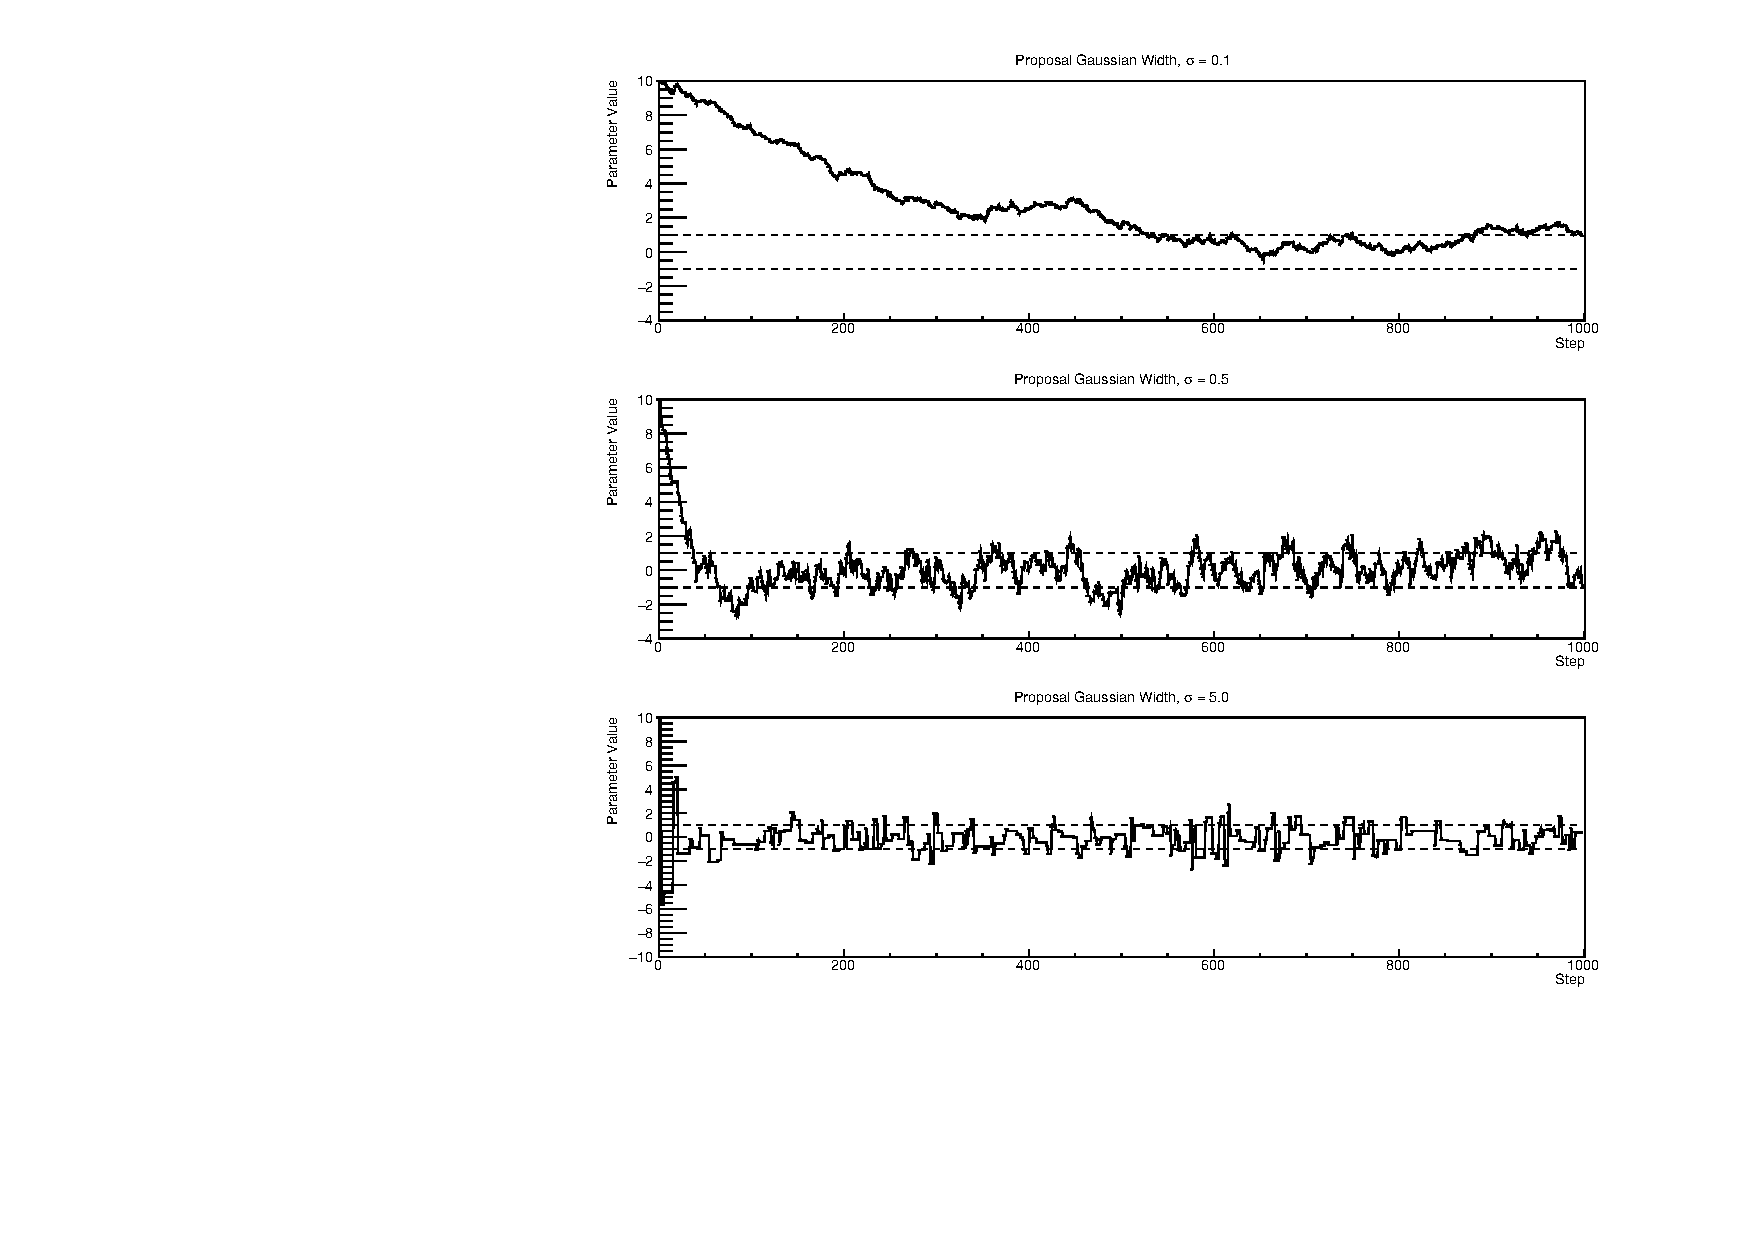
\includegraphics[width=\textwidth, trim={10mm 0mm 18mm 0mm}, clip,page=1]{Figures/MCMC/MCMCTechnique_StepSizes.pdf}
  \end{subfigure}
  \caption{Three MCMC chains, each with a stationary distribution equal to a Gaussian centered at \quickmath{0} and width \quickmath{1} (As indicated by the black dotted lines). All of the chains use a Gaussian proposal function but have different widths (or `step size \quickmath{\sigma}'). The top panel has \quickmath{\sigma = 0.1}, middle panel has \quickmath{\sigma = 0.5} and the bottom panel has \quickmath{\sigma = 5.0}.}
  \label{fig:MCMC_MCTechniqueStepSizeStudy}
\end{figure}

As discussed, step size tuning directly correlates to the average step acceptance rate. If the step size is too small, many steps will be accepted but the chain moves slowly. If the opposite is true, many steps will be rejected as the chain proposes steps in the tails of the distribution. Discussion in \cite{Dunkley2005-xz} suggests that the `ideal' acceptance rate of a high dimension MCMC chain should be approximately \quickmath{\sim 25\%}. An ``ideal'' step size \cite{Dunkley2005-xz} of

\begin{equation}
  \label{eq:MCMC_IdealStepSize}
  \sigma = \frac{2.4}{N_{p}},
\end{equation}

where \quickmath{N_{p}} is the number of parameters included in the MCMC fit. However, the complex correlations between systematics mean that some parameters have to be hand-tuned and many efforts have been taken to select a set of parameter-by-parameter step sizes to approximately reach the ideal acceptance rate.

\autoref{fig:MCMC_MCTechniqueLLHVsStep} highlights the likelihood as calculated by the fit in \finish{Link to AsimovA Sensitivity Section} as a function of the number of steps in each chain. In practice, many independent MCMC chains are run simultaneously to parallelise the task of performing the fit. This figure overlays the distribution found in each chain. As seen, the likelihood decreases from its initial value and converges towards a stationary distribution after \quickmath{\sim 1 \times 10^{5}} steps.

\begin{figure}[h]
  \begin{subfigure}[t]{0.8\textwidth}
    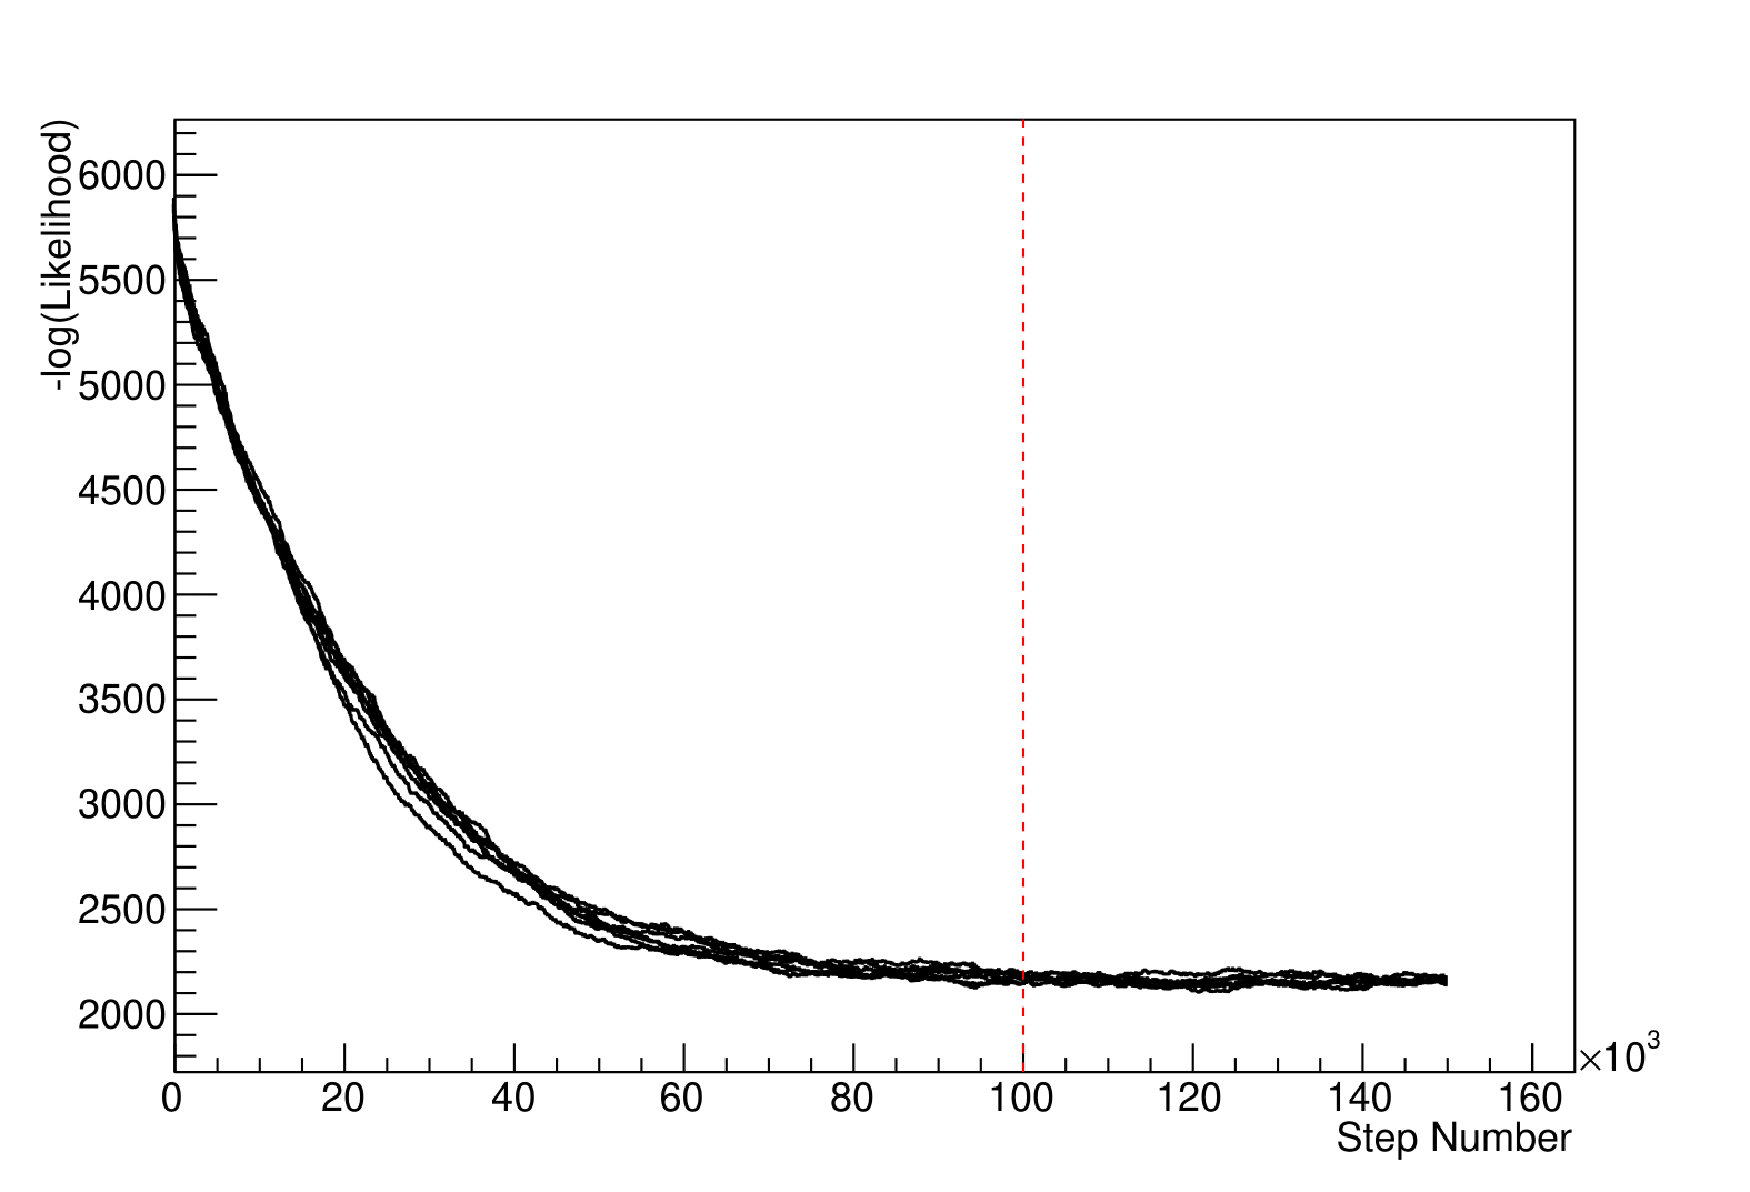
\includegraphics[width=\textwidth, trim={0mm 0mm 0mm 0mm}, clip,page=1]{Figures/MCMC/MCTechnique_LLHStep.pdf}
  \end{subfigure}
  \caption{The log-likelihood from the fit detailed in \finish{Link to AsimovA Sensitivity Section} as a function of the number of steps accumulated in each fit. Many independent MCMC chains were run in parallel and overlaid on this plot. The red line indicates the \quickmath{1 \times 10^{5}} step burn-in period after which the log-likelihood becomes stable.}
  \label{fig:MCMC_MCTechniqueLLHVsStep}
\end{figure}

Multiple configurations of this analysis have been performed throughout this thesis where different samples or systematics have been used. For all of these configurations, it was found that a burnin period of \quickmath{1 \times 10^{5}} was sufficient in all cases.

\section{Understanding the MCMC Results}
\label{sec:MarkovChainMonteCarlo_UnderstandingMCMCResults}

The previous sections have described how to generate the posterior probability distribution using Bayesian MCMC techniques. However, this analysis focuses on oscillation parameter determination. The posterior distribution output from the chain is a high-dimension object, with as many dimensions as there are parameters included in the oscillation analysis. However, this multi-dimensional object is difficult to conceptualize so parameter estimations are often presented in one or two-dimensional projections of this probability distribution. To do this, we invoke the marginalisation technique highlighted in \autoref{sec:MarkovChainMonteCarlo_Marginalisation}.

\subsection{Marginalisation}
\label{sec:MarkovChainMonteCarlo_Marginalisation}

The output of the MCMC chain is a highly dimensional probability distribution which is very difficult to interpret. From the standpoint of an oscillation analysis experiment, the one or two-dimensional `projections' of the oscillation parameters of interest are most relevant. Despite this, the best fit values and uncertainties on the oscillation parameters of interest should correctly encapsulate the correlations to the other systematic uncertainties (colloquially called `nuisance' parameters). For this joint beam and atmospheric analysis, the oscillation parameters of interest are \quickmath{\sin^{2}(\theta_{23})}, \quickmath{\sin^{2}(\theta_{13})}, \quickmath{\Delta m^{2}_{32}}, and\quickmath{\delta_{CP}}. All other parameters (including the oscillation parameters this fit is insensitive to) are deemed nuisance parameters. To generate these projections, we rely upon integrating the posterior distribution over all nuisance parameters. This is called marginalisation. This technique also explains why it is acceptable to neglect the normalisation constant of the posterior distribution, which was discussed in \autoref{sec:MarkovChainMonteCarlo_BayesianStatistics}.

A simple example of the marginalisation technique is to imagine the scenario where two coins are flipped. To determine the probability that the first coin returned a `head', the exact result of the second coin flip is disregarded and simply integrated over. For the parameters of interest, \quickmath{\vec{\theta}_{i}}, we can calculate the marginalised posterior by integrating over the nuisance parameters, \quickmath{\vec{\theta}_{n}}. In this case, \autoref{eq:MarkovChainMonteCarlo_PosteriorDistribution} becomes

\begin{equation}
P(\vec{\theta}_{i}|D) = \frac{\int P(D|\vec{\theta}_{i},\vec{\theta}_{n}) P(\vec{\theta}_{i},\vec{\theta}_{n}) d\vec{\theta}_{n}}{\int P(D|\vec{\theta}) P(\vec{\theta}) d\vec{\theta}}
\end{equation}

Where \quickmath{P(\vec{\theta}_{i},\vec{\theta}_{n})} encodes the prior knowledge about the uncertainty and correlations between the parameters of interest and the nuisance parameters. In practice, this is simply taking the one or two-dimensional projection of the multi-dimensional probability distribution.

While in principle an easy solution to a complex problem, correlations between the interesting and nuisance parameters can bias the marginalised results. A similar effect is found when the parameters being marginalised over have non-Gaussian probability distributions. For example, \autoref{fig:MCMC_MCTechniqueMarginalisationProblems} highlights the marginalisation bias in the probability distribution found for a parameter when requiring a correlated parameter to have a positive parameter value. Due to the complex nature of the oscillation parameter fit presented in this thesis, there are correlations occurring between the oscillation parameters of interest and the other nuisance parameters included in the fit.

\begin{figure}[h]
  \begin{subfigure}[t]{0.48\textwidth}
    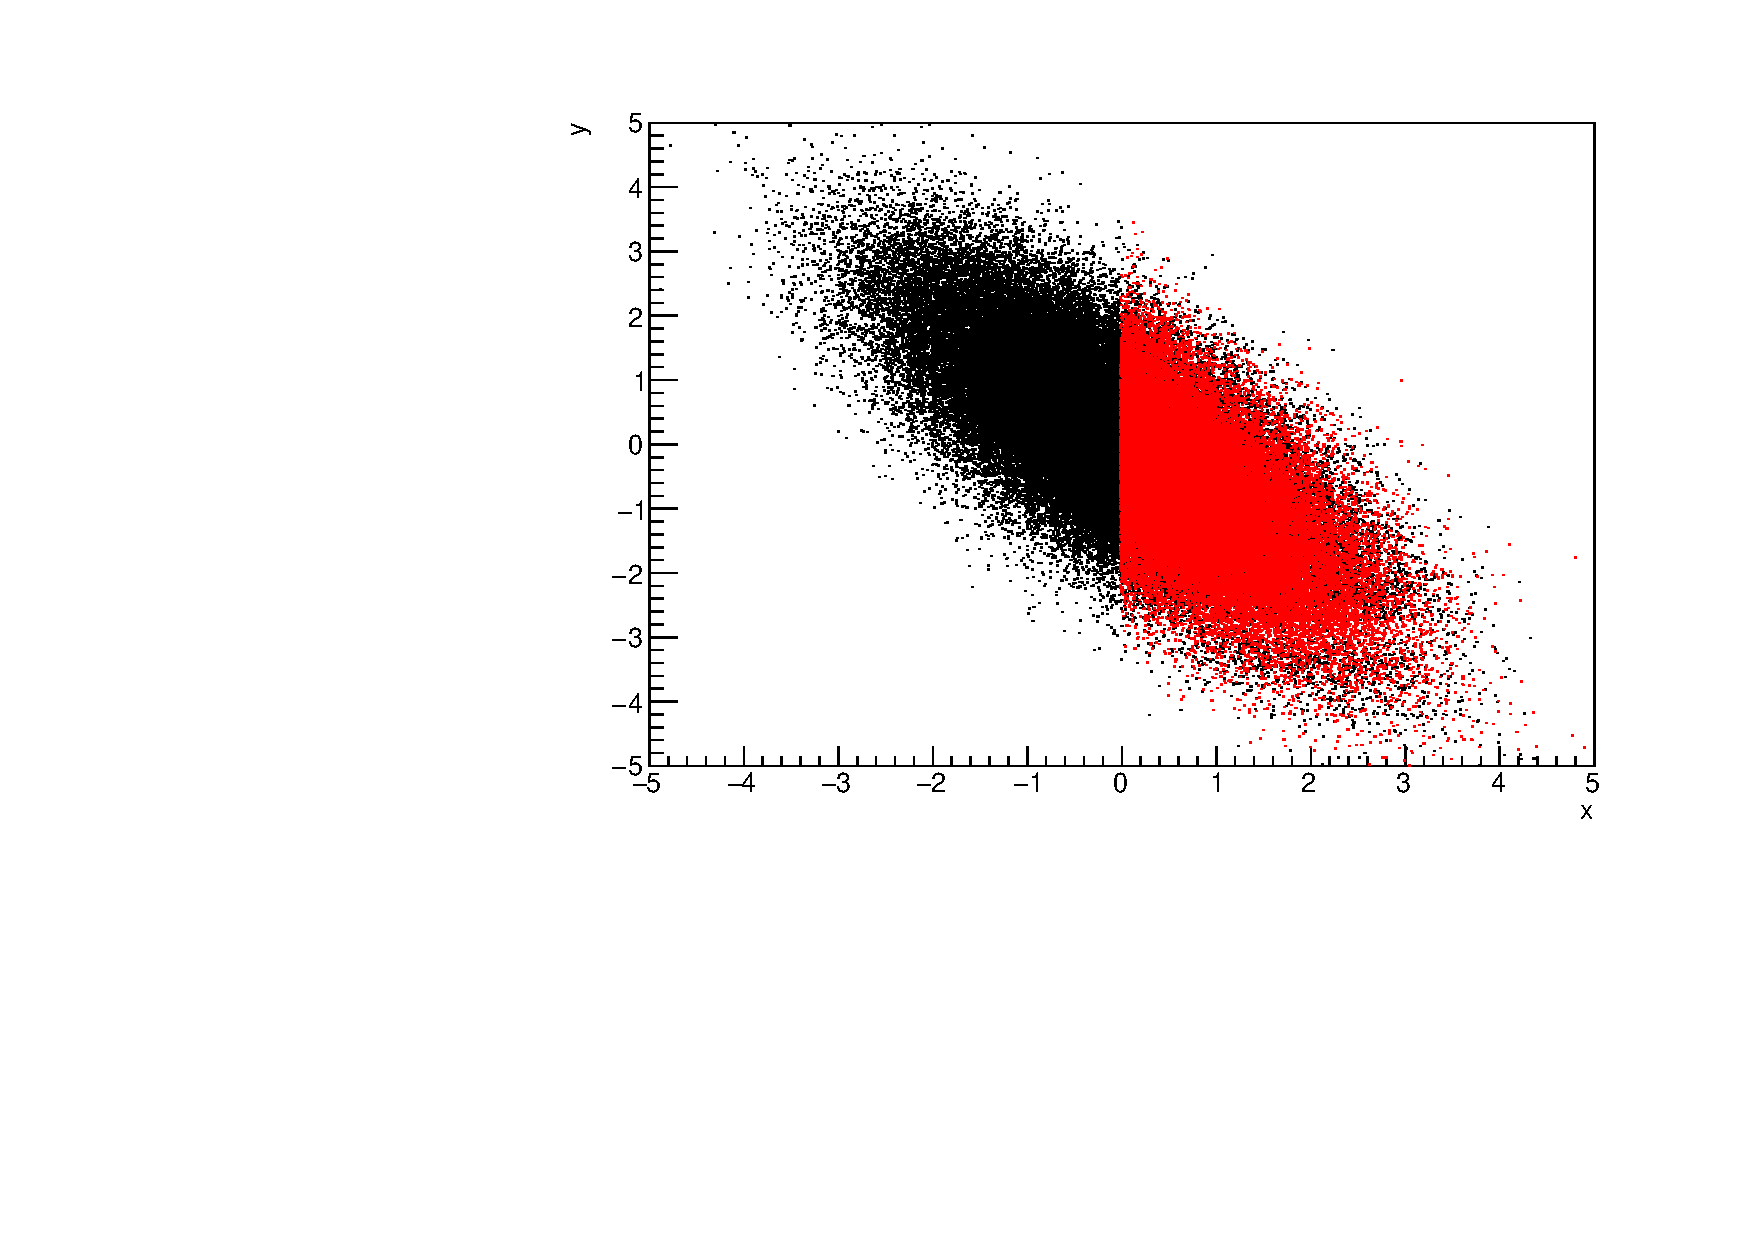
\includegraphics[width=\textwidth, trim={0mm 0mm 0mm 0mm}, clip,page=1]{Figures/MCMC/MCTechnique_Marginalisation2D_Double_Correlations.pdf}
  \end{subfigure} %
    \begin{subfigure}[t]{0.48\textwidth}
    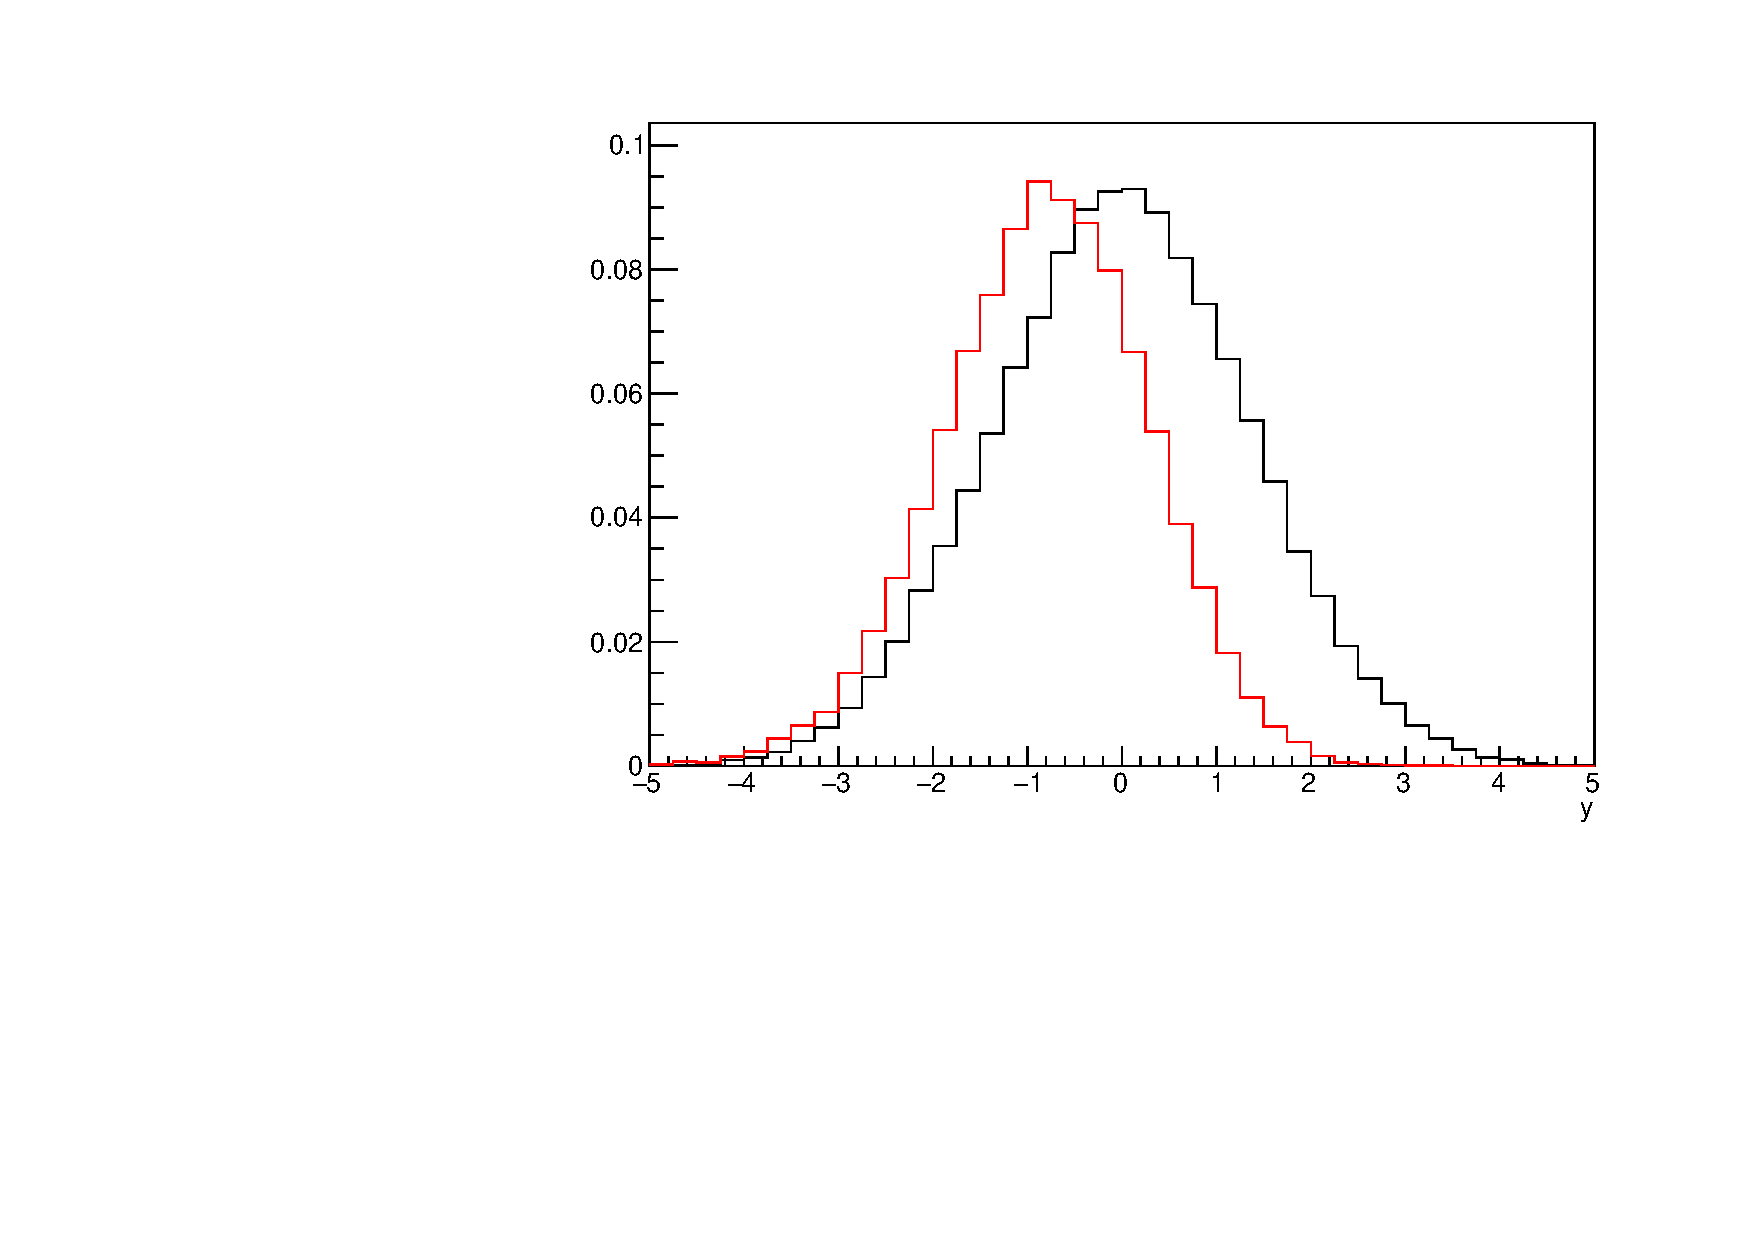
\includegraphics[width=\textwidth, trim={0mm 0mm 0mm 0mm}, clip,page=1]{Figures/MCMC/MCTechnique_Marginalisation1D_Double_Correlations.pdf}
  \end{subfigure}

  \caption{Left: The two-dimensional probability distribution for two correlated parameters \quickmath{x} and \quickmath{y}. The red distribution shows the two-dimensional probability distribution when \quickmath{0 \leq x \leq 5}. Right: The marginalised probability distribution for the \quickmath{y} parameter found when requiring the \quickmath{x} to be bound between \quickmath{-5 \leq x \leq 5} and \quickmath{0 \leq x \leq 5} for the black and red distribution, respectively.}
  \label{fig:MCMC_MCTechniqueMarginalisationProblems}
\end{figure}

\subsection{Parameter Estimation and Credible Intervals}
\label{sec:MarkovChainMonteCarlo_ParameterEstimation}

The purpose of this analysis is to determine the best fit values for the oscillation parameters that the beam and atmospheric samples are sensitive to: \quickmath{\sin^{2}(\theta_{23})}, \quickmath{\sin^{2}(\theta_{13})}, \quickmath{\Delta m^{2}_{32}}, and \quickmath{\delta_{CP}}.
%Typically, the results presented take the form of one or two-dimension marginalised probability distributions for the appearance (\quickmath{\sin^{2}(\theta_{13})} and \quickmath{\delta_{CP}}) and disappearance (\quickmath{\sin^{2}(\theta_{23})} and \quickmath{\Delta m^{2}_{32}}) parameters.
The posterior probability density, taken from the output MCMC chain, is binned in these parameters. The parameter best-fit point is then taken to be the value that has the highest posterior probability. This is performed in both one and two-dimensional projections.

However, the single best-fit point in a given parameter is not of much use on its own. We would also like to determine the uncertainty, or credible interval, on that best-fit point. The definition of the \quickmath{1\sigma} credible interval is that we have \quickmath{68\%} belief that the parameter is within those bounds. For a more generalised definition, the credible interval is the region, \quickmath{R}, of the posterior distribution that contains a specific fraction of the total probability, such that

\begin{equation}
\int_{R} P(\theta|D)d\theta = \alpha
\end{equation}

Where \quickmath{\theta} is the parameter on which we calculate the credible interval. This technique then calculates the \quickmath{\alpha \times 100\%} credible interval.

In practice, this analysis uses the highest posterior density (HPD) credible intervals which are calculated through the following method. First, the probability distribution is area-normalised such that it has an integrated area equal to \quickmath{1.0}. The bins of probability are then summed from the highest to lowest until the sum exceeds the \quickmath{1\sigma} level (\quickmath{0.68} in this example). This process is repeated for a range of credible intervals, notably the \quickmath{1\sigma}, \quickmath{2\sigma} and \quickmath{3\sigma} along with other levels where the critical values for each level can be found in \cite{Particle_Data_Group2020-ms}. This process can be repeated for the two-dimensional probability distributions by creating two-dimensional contours of credible intervals rather than a one-dimensional result. 

\subsection{Bayesian Model Comparisons}
\label{sec:MarkovChainMonteCarlo_BayesTheorem}
Due to the matter resonance, this analysis has some sensitivity to the mass hierarchy of neutrino states (whether \quickmath{\Delta m^{2}_{32}} is positive or negative) and the octant of \quickmath{\sin^{2}(\theta_{23})}. The Bayesian approach utilised within this analysis gives an intuitive method of model comparison by determining which hypothesis is most favourable. Taking the ratio of \autoref{eq:MarkovChainMonteCarlo_PosteriorDistributionReduced} for the two hypotheses of normal hierarchy, \quickmath{NH}, and inverted hierarchy, \quickmath{IH}, gives

\begin{equation}
  \frac{P(\vec{\theta}_{NH}|D)}{P(\vec{\theta}_{IH}|D)} = \frac{P(D|\vec{\theta}_{NH})}{P(D|\vec{\theta}_{IH})} \times \frac{P(\vec{\theta}_{NH})}{P(\vec{\theta}_{IH})}.
\end{equation}

The middle term defines the Bayes factor, \quickmath{B(\text{NH}/\text{IH})}, which is a data-driven interpretation of how strong the data prefers one hierarchy to the other. For this analysis, equal priors on both mass hierarchy hypotheses are chosen (\quickmath{P(\vec{\theta}_{NH}) = P(\vec{\theta}_{IH})} = 0.5). In practice, the MCMC chain proposes a value of \quickmath{|\Delta m^{2}_{32}|} and then applies a \quickmath{50\%} probability that the value is sign flipped. Consequently, the Bayes factor can be calculated from the ratio of the probability density in either hypothesis. This equates to counting the number of steps taken in the normal and inverted hierarchies and taking the ratio. The same approach can be taken to compare the upper octant (UO) compared to the lower octant (LO) hypothesis of \quickmath{\sin^{2}(\theta_{23})}.

\begin{table}[ht!]
    \centering
    \begin{tabular}{c|c|l}
      \hline
      $\log_{10}(B_{AB})$ & $B_{AB}$ & Strength of Preference \\
      \hline
      \hline
      \quickmath{<0.0} & \quickmath{<1} & No preference for hypothesis A (Supports hypothesis B) \\
      \quickmath{0.0 - 0.5} & \quickmath{1.0 - 3.16} & Preference for hypothesis A is weak \\
      \quickmath{0.5 - 1.0} & \quickmath{3.16 - 10.0} & Preference for hypothesis A is substantial \\
      \quickmath{1.0 - 1.5} & \quickmath{10.0 - 31.6} & Preference for hypothesis A is strong \\
      \quickmath{1.5 - 2.0} & \quickmath{31.6 - 100.0} & Preference for hypothesis A is very strong \\
      \quickmath{>2.0 }& \quickmath{>100.0} & Decisive preference for hypothesis A \\
      \hline
      \hline
      
      \hline
    \end{tabular}
    \caption{Jeffreys scale for strength of preference for two models \quickmath{A} and \quickmath{B} as a function of the calculated Bayes factor (\quickmath{B_{AB} = B(A/B)}) between the two models \cite{Jeffreys:1939xee}. The original scale is given in terms of \quickmath{\log_{10}(B(A/B))} but converted to linear scale for easy comparison throughout this thesis.}
    \label{tab:MarkovChainMonteCarlo_JeffreysScale}
\end{table}

Whilst the value of the Bayes factor should always be shown, the Jeffreys scale \cite{Jeffreys:1939xee} (highlighted in \autoref{tab:MarkovChainMonteCarlo_JeffreysScale}) gives an indication of the strength of preference for one model compared to the other. Other interpretations of the strength of preference of a model exist, e.g. the Kass and Raferty Scale \cite{Kass1995-nl}.

\subsection{Comparison of MCMC Output to Expectation}
\label{sec:MarkovChainMonteCarlo_Predictives}

To ensure the fit is performing well, a best-fit spectrum is produced using the posterior probability distribution and compared with the data, allowing easy by-eye comparisons to be made. A simple method of doing this is to perform a comparison in the fitting parameters (For instance, the reconstructed neutrino energy and lepton direction for T2K far detector beam samples) of the spectra generated by the MCMC chain to `data'. This `data' could be true data or some variation of Monte Carlo prediction. This allows easy comparison of the MCMC probability distribution to the data. To perform this, \quickmath{N} steps from the post-burnin MCMC chain are randomly selected. From these, the Monte Carlo prediction at each step is generated by reweighting the model parameters to the values specified at that step. Due to the probability density being directly correlated with the density of steps in a certain region, parameter values close to the best fit value are most likely to be selected.

In practice, for each bin of the fitting parameters has a probability distribution of event rates, with one entry per sampled MCMC step. This distribution is binned where the bin with the highest probability is selected as the mean and an error on the width of this probability distribution is calculated using the approach highlighted in \autoref{sec:MarkovChainMonteCarlo_ParameterEstimation}. Consequently, the best fit distribution in the fit parameter is not necessarily that which would be attained by reweighting the Monte Carlo prediction to the most probable parameter values.

A similar study can be performed to illustrate the freedom of the model parameter space prior to the fit. This can be done by throwing parameter values from the prior uncertainty of each parameter.
%This becomes troublesome for parameters with no prior uncertainty as the range is technically infinite. Where applicable solutions to remove these have been addressed.

  \chapter{Simulation, Reconstruction, and Event Reduction}
\label{chap:Simulations}

As a crucial part of the oscillation analysis, an accurate prediction of the expected neutrino spectrum at the far detector is required. This includes modeling the flux generation, neutrino interactions, and detector effects. All of the simulation packages required to do this are briefly described in \autoref{sec:Simulations_Simulation}. The reconstruction of neutrino events inside the far detector, including the \fq algorithm, is documented in \autoref{sec:Simulation_Reconstruction}. This also includes data quality checks of the SK-V data which the author performed for the T2K oscillation analysis presented at Neutrino 2020 \cite{Dunne2020-uf}. Finally, \autoref{sec:Simulations_Reduction} describes the steps taken in the SK detector to trigger on events of interest whilst removing the comparatively large rate of cosmic ray muon events.

\section{Simulation}
\label{sec:Simulations_Simulation}

In order to generate a Monte Carlo prediction of the expected event rate at the far detector, all the processes in the beam and atmospheric flux, neutrino interaction, and detector need to be modeled. Each of these parts is individually modeled and each of them is detailed below.

The beamline simulation consists of three distinct parts: the initial hadron interaction modeled by FLUKA \cite{fluka2011}, the target station geometry and particle tracking performed by JNUBEAM, \cite{geant3, PhysRevD.87.012001} and any hadronic re-interactions simulated by GCALOR \cite{gcalor}. The primary hadronic interactions are \quickmath{O(10)\text{GeV}}, where FLUKA matches external cross-section data better than GCALOR \cite{t2k_tn_flux}. However, FLUKA is not very adaptable so a small simulation is built to model the interactions in the target and the output is then passed to JNUBEAM and GCALOR for propagation. The hadronic interactions are tuned to data from the NA61/SHINE \cite{Abgrall_2011, Abgrall_2012, NA61_pions_rep} and HARP \cite{harp} experiments. The tuning is done by reweighting the FLUKA and GCALOR predictions to match the external data multiplicity and cross-section measurements, based on final state particle kinematics \cite{t2k_tn_flux}. The culmination of this simulation package generates the predicted flux for neutrino and antineutrino beam modes which are illustrated in \autoref{fig:T2KSKExp_T2K_NuFluxPerMode}.

The atmospheric neutrino flux predictions are simulated by the HKKM model \cite{Honda_2007, Honda:2011}. The primary cosmic ray flux is tuned to AMS \cite{Blau2002} and BESS \cite{Haino2004} data assuming the US-standard atmosphere `76 \cite{USStandardAtm} density profile and includes geomagnetic field effects. The primary cosmic rays interact to generate pions and muons. The interaction of these secondary particles to generate neutrinos is handled by DPMJET-III \cite{Roesler2001} for energies above \quickmath{32\text{GeV}} and JAM \cite{Niita2006, Honda:2011} for energies below that value \finish{Question for Giles: Why different generators for above/below 32GeV?}. These hadronic interactions are tuned to BESS and L3 data \cite{Sanuki_2002, Achard_2004} using the same methodology as the tuning of the beamline simulation. The energy and cosine zenith predictions of \quickmath{\nu_{e}, \bar{\nu}_{e}, \nu_{\mu}, \bar{\nu}_{\mu}} flux are given in \autoref{fig:NeutrinoOscillationPhysics_AtmosphericNeutrinoFlux} and \autoref{fig:NeutrinoOscillationPhysics_NuFluxZenithAngleDep}, respectively. The flux is approximately symmetrical and peaked around the horizon (\quickmath{\cos(\theta_{Z}) = 0.0}). This is because horizontally-going pions and kaons can travel further than their vertically-going counterparts resulting in a larger probability of decaying to neutrinos. The symmetry is broken in low-energy neutrinos due to geomagnetic effects, which modify the track of the primary cosmic rays. Updates to the HKKM model are currently ongoing \cite{Sato2022-ss}.

Once a flux prediction has been made for all three detectors, NEUT 5.4.0 \cite{Hayato2021, neut} models the interactions of the neutrinos in the detectors. For the purposes of this analysis, quasi-elastic (QE), meson exchange (MEC), single meson production (PROD), coherent pion production (COH), and deep inelastic scattering (DIS) interactions are simulated. These interaction categories can be further broken down by whether they were propagated via a \quickmath{W^{\pm}} boson in Charged Current (CC) interactions or via a \quickmath{Z^{0}} boson in Neutral Current (NC) interactions. CC interactions have a charged lepton in the final state, which can be flavour-tagged in reconstruction to determine the flavour of the neutrino. In contrast, NC interactions have a neutrino in the final state so no flavour information can be determined from the observables left in the detector after an interaction. This is the reason why NC events are assumed to not oscillate within this analysis. Both CC and NC interactions are modeled for all the above interaction categories, other than MEC interactions which are only modeled for CC events. The SK detector is only sensitive to charged particles, so all charged current interactions are simulated whilst only neutral current processes that produce charged mesons (NCDIS, NCCOH, and NCPROD) are modeled. NC MEC interactions can only produce charged particles through secondary re-interactions which is a low cross-section process.

\begin{figure}[h]
  \begin{subfigure}[t]{0.8\textwidth}
    \includegraphics[width=\textwidth, trim={0mm 0mm 0mm 0mm}, clip,page=1]{Figures/Simulations/NEUTCrossSection.pdf}
  \end{subfigure}
  \caption{The NEUT prediction of the \quickmath{\nu_{\mu}}-H2O cross-section overlaid on the T2K \quickmath{\nu_{\mu}} flux. The charged current (black, solid) and neutral current (black, dashed) inclusive, charged current quasi-elastic (blue, solid), charged current 2p2h (blue, dashed), charged current single pion production (pink), and charged current multi--\quickmath{\pi} and DIS (Purple) cross-sections are illustrated. Figure taken from \cite{Hayato2021}.}
  \label{fig:Simulations_CrossSection}
\end{figure}

As illustrated in \autoref{fig:Simulations_CrossSection}, CC QE interactions dominate the low-energy cross-section of neutrino interactions. The NEUT implementation adopts the Llewellyn Smith \cite{llewelyn-smith} model for neutrino-nucleus interactions, where the nuclear ground state of any bound nucleons (neutrino-oxygen interactions) is approximated by a spectral-function \cite{Benhar1989} model that simulates the effects of Fermi momentum and Pauli blocking. The cross-section of QE interactions are controlled by vector and axial-vector form factors parameterised by the BBBA05 \cite{bbba05} model and a dipole form factor with \quickmath{M_{A}^{QE} = 1.21\text{GeV}} fit to external data \cite{Aguilar_Arevalo_2010}, respectively. NEUT implements the Valencia \cite{nieves2} model to simulate MEC events, where two nucleons and two holes in the nuclear target are produced (Often called 2p2h interactions).

For neutrinos of energy \quickmath{O(1)\text{GeV}}, PROD interactions become dominant. These predominantly produce charged and neutral pions although \quickmath{\gamma}, kaon, and \quickmath{\eta} production is also considered. To simulate these interactions, the Berger-Sehgal \cite{PhysRevD.76.113004} model is implemented within NEUT. It simulates the excitation of a nucleon from a neutrino interaction, production of an intermediate baryon, and the consequential decay to a single meson or \quickmath{\gamma}. Pions can also be produced through COH interactions, which occur when the incoming neutrino interacts with the entire oxygen nuclei target leaving a single pion outside of the nucleus. NEUT utilises the Berger-Sehgal \cite{Berger_Sehgal_coh} model to simulate these COH interactions.

DIS and multi-\quickmath{\pi} producing interactions become the most dominant for energies \quickmath{>O(5)\text{GeV}}. PYTHIA \cite{Sjstrand1994} is used to simulate any interaction with invariant mass, \quickmath{W > 2\text{GeV/c}^{2}}, which produces at least one meson. For any interaction which produces at least two mesons but has \quickmath{W < 2\text{GeV/c}^{2}}, the Bronner model is invoked \cite{Bronner2016}. Both of these models use Parton distribution functions based on the Bodek-Yang model \cite{Gl_ck_1998,10.48550/arxiv.1011.6592,10.48550/arxiv.1012.0261}. 

\begin{figure}[h]
  \begin{subfigure}[t]{0.8\textwidth}
    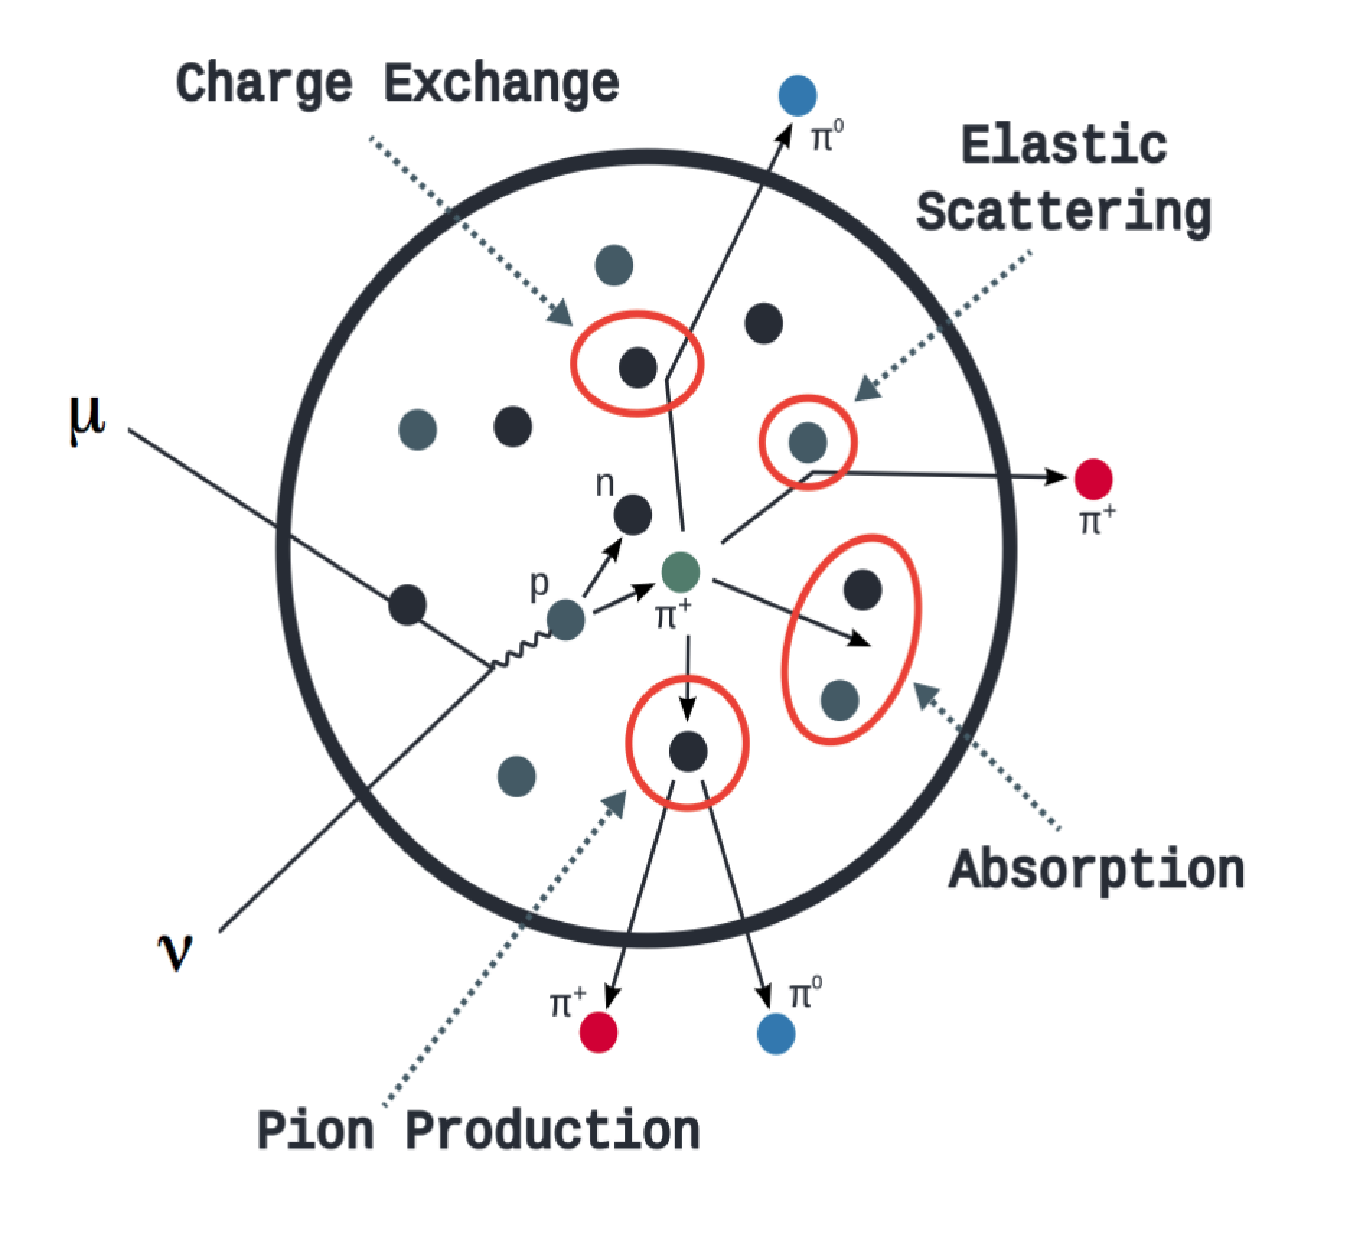
\includegraphics[width=\textwidth, trim={0mm 0mm 0mm 0mm}, clip,page=1]{Figures/Simulations/FSIDiagram.pdf}
  \end{subfigure}
  \caption{Illustration of the various processes which a pion can undergo before exiting the nucleus. Taken from \cite{10.48550/arxiv.1602.05299}.}
  \label{fig:Simulations_FSIDiagram}
\end{figure}

Any pion which is produced within the nucleus can re-interact through final state interactions before it exits, as illustrated by the scattering, absorption, production, and exchange interactions in \autoref{fig:Simulations_FSIDiagram}. These re-interactions alter the observable particles within the detector. For instance, if the charged pion from a CC PROD interaction is absorbed, the observables would mimic a CC QE interaction. To simulate these effects, NEUT uses a semi-classical intranuclear cascade model \cite{Hayato2021}. This cascade functions by stepping the pion through the nucleus in fixed-length steps equivalent to \quickmath{dx = R_{N}/100}, where \quickmath{R_{N}} is the radius of the nucleus. At each step, the simulation allows the pion to interact through scattering, charged exchange, absorption, or production with an interaction-dependent probability calculated from a fit to external data \cite{PhysRevD.99.052007}. This cascade continues until the pion is absorbed or exits the nucleus.

Once the final state particle kinematics have been determined from NEUT, they are passed into the detector simulation. The near detectors, ND280 and INGRID, are simulated using a \texttt{GEANT4} package \cite{t2k_det,geant4} to simulate the detector geometry, particle tracking, and energy deposition. The response of the detectors is simulated using the elecSim package \cite{t2k_det}. The far detector simulation is based upon the original Kamiokande experiment software which uses the \texttt{GEANT3}-based SKDETSIM \cite{Brun:1987ma,t2k_det} package. This controls the interactions of particles in the water as well as Cherenkov light production. The water quality and PMT calibration measurements detailed in \autoref{subsec:T2KSKExp_SKCalibration} are also used within this simulation to make accurate predictions of the detector response.

\section{Event Reconstruction at SK}
\label{sec:Simulation_Reconstruction}

Any above Cherenkov threshold event which occurs in SK will be recorded by the PMT array, where each PMT records the time and accumulated charge. This recorded information is shown in event displays similar to those illustrated in \autoref{fig:Simulations_SKEventDisplays}. To be useful for physics analyses, this series of PMT hit information needs to be reconstructed to determine the particle's identity and kinematics (or track parameters): four-vertex, direction, and momenta. This is because the charge and timing distribution of photons generated by a particular particle in an event is dependent upon its initial kinematics. The concept of distinguishing electron and muon events is from the ``fuzziness'' of the ring. Muons are heavier and less affected by scattering or showering meaning they typically produce ``crisp'' rings. Electrons are more likely to interact via electromagnetic showering or scattering which results in larger variations of their direction from the initial direction. Consequently, electrons typically produce ``fuzzier'' rings compared to muons. 

For the purposes of this analysis, the \fq reconstruction algorithm is utilised. Its core function is to compare a prediction of the accumulated charge and timing distribution from each PMT, generated for a particular particle identity and track parameters, to that observed in the neutrino event. It determines the preferred values by minimising a likelihood function which includes information from PMTs which were hit and those that were not hit. The \fq algorithm improves upon the \apfit reconstruction algorithm which has been used for many previous SK analyses.
\apfit fits the vertex from timing information and then fits the momentum and direction of the particle from PMT hits within a \quickmath{43\deg} Cherenkov cone (which assumes an ultra-relativistic particle). It then fits the particle identity once the track parameters have been fit. Conversely, \fq performs a simultaneous fit of particle kinematics and identity, improving both the accuracy of the fit parameters and the rejection of neutral current \quickmath{\pi^{0}} events \cite{Abe2018, Abe2015}. The \fq algorithm is based on the key concepts of the MiniBooNE reconstruction algorithm \cite{Patterson_2009} and is described in \cite{t2k_tn_146} which is summarised below.

\begin{figure}[h]
  \begin{subfigure}[t]{0.5\textwidth}
    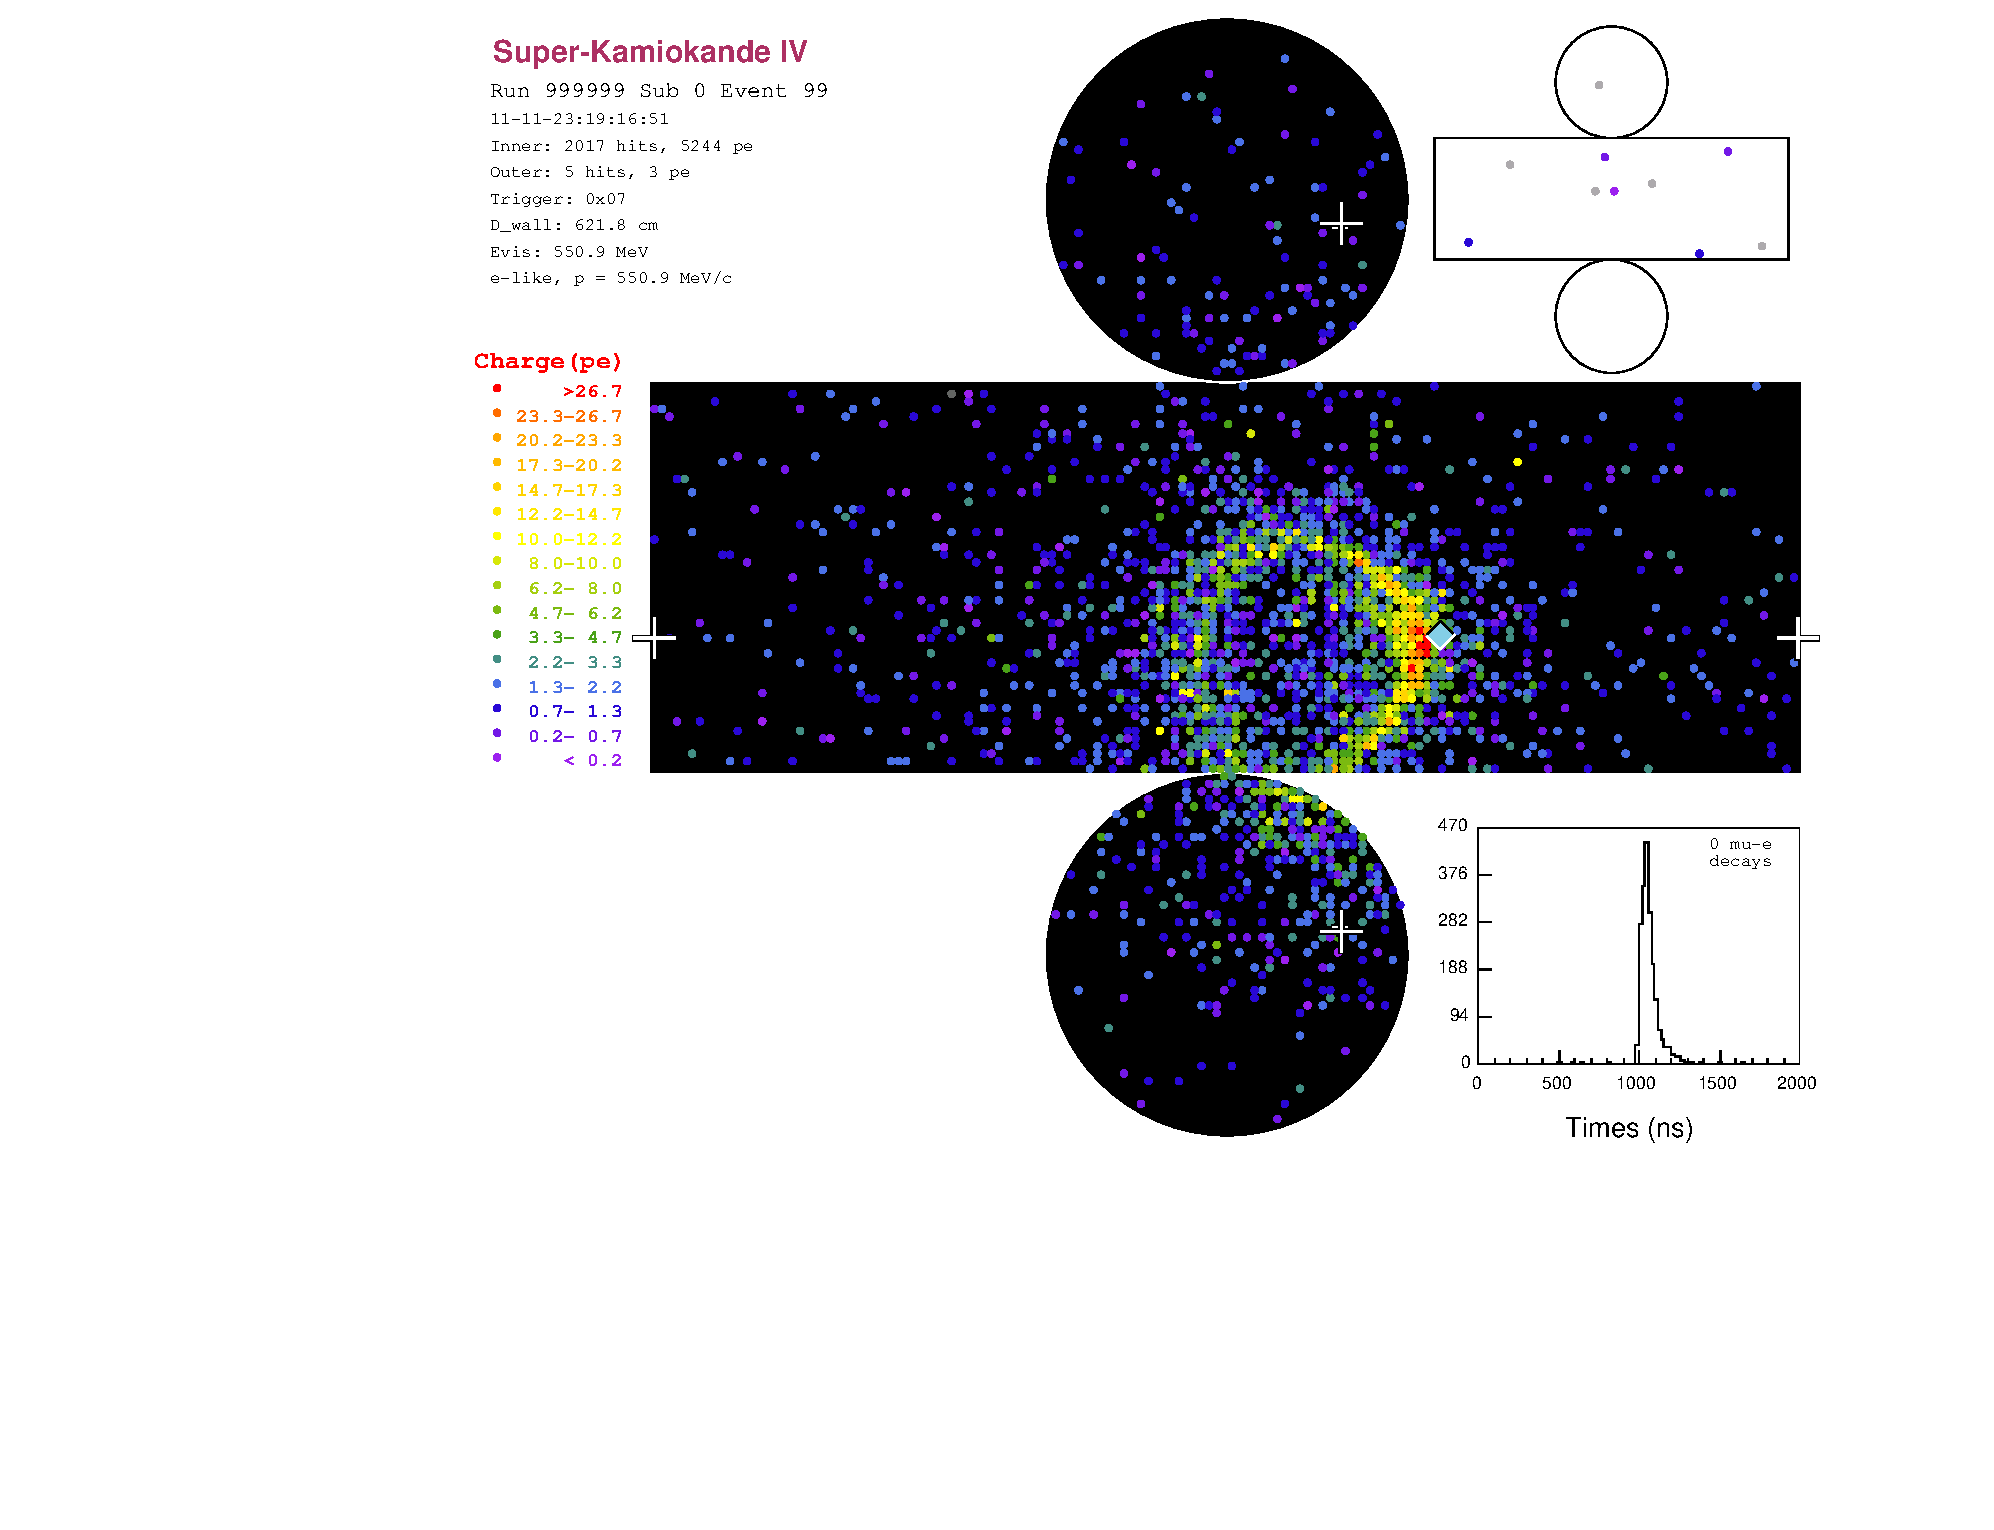
\includegraphics[width=\textwidth, trim={0mm 0mm 0mm 0mm}, clip,page=1]{Figures/Simulations/NuECandidate.pdf}
    \subcaption{\quickmath{\nu_{e}}}
  \end{subfigure}%
  \begin{subfigure}[t]{0.5\textwidth}
    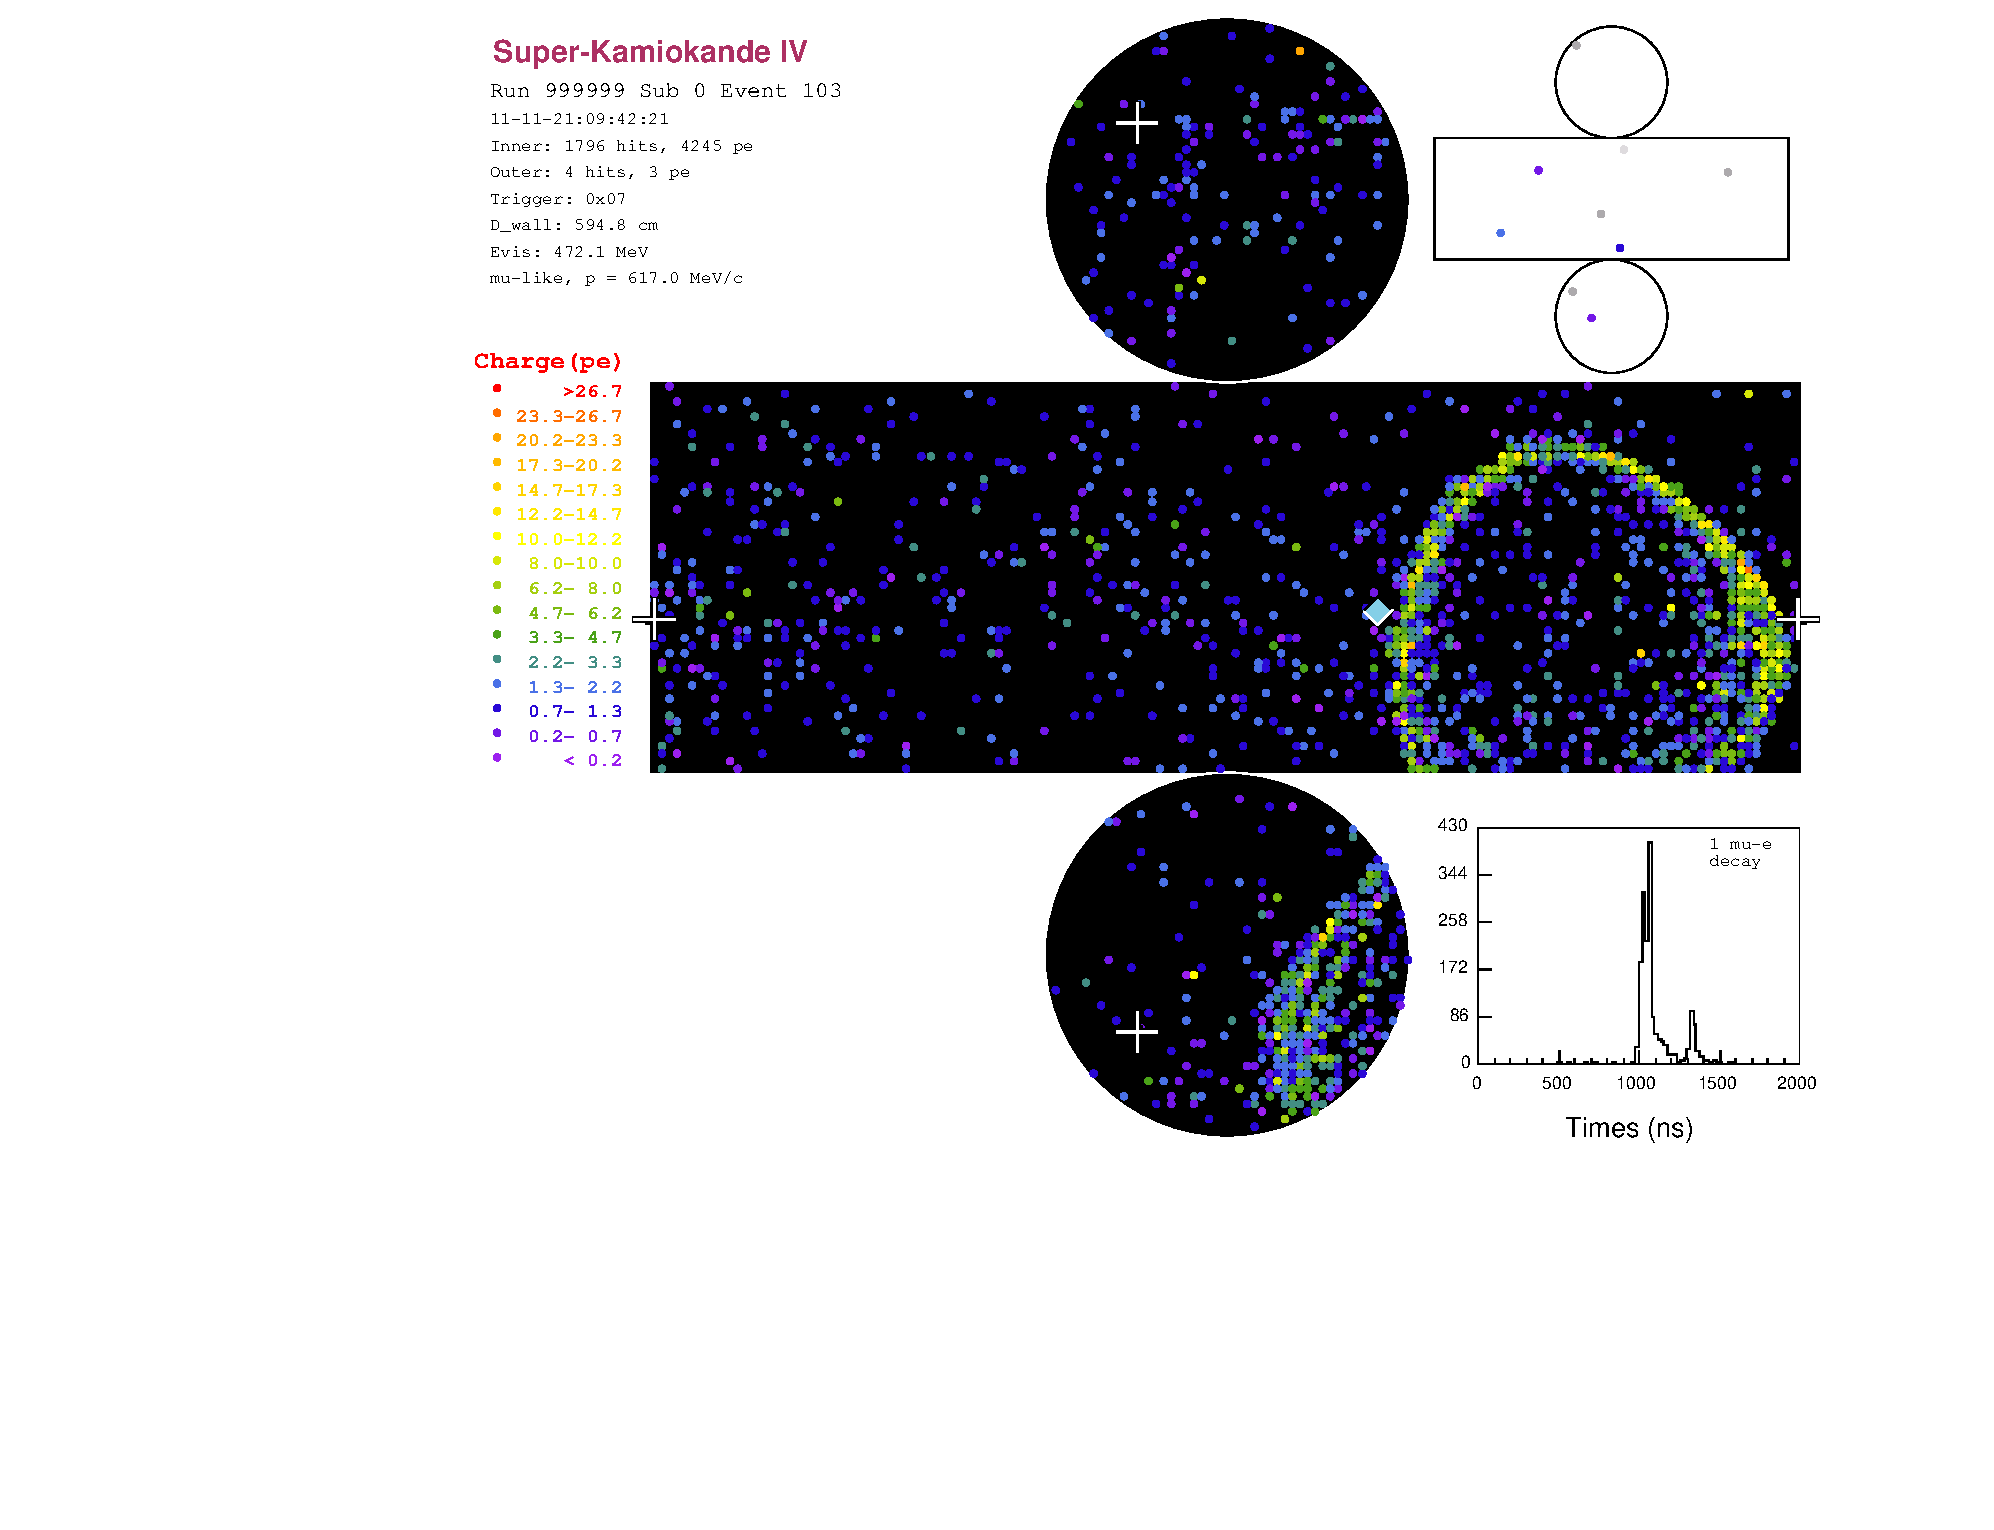
\includegraphics[width=\textwidth, trim={0mm 0mm 0mm 0mm}, clip,page=1]{Figures/Simulations/NuMuCandidate.pdf}
    \subcaption{\quickmath{\nu_{\mu}}}
  \end{subfigure}
  \caption{Event displays from Super Kamiokande illustrating the ``crisp'' ring from a muon and the typically ``fuzzier'' electron ring. Each pixel represents a PMT and the color scheme denotes the accumulated charge deposited on that PMT. Figures taken from \cite{t2k_tn_219}.}
  \label{fig:Simulations_SKEventDisplays}
\end{figure}

%An event in SK can consist of multiple ``sub-events''. For example, a muon neutrino interaction will generate a muon which will subsequently decay into an electron. Both the muon and electron can generate Cherenkov photons but both subevents need to be reconstructed separately. Therefore, to avoid assigning photons generated by the decay-electron to the muon, each event is divided into time clusters, termed ``subevents'', where subevent is defined to contain at most one hit for each PMT. To find the subevents, a vertex goodness metric is calculated for some vertex position \quickmath{\vec{x}} and time \quickmath{t},

An event in SK can consist of multiple particles. For example, a charge current muon neutrino interaction can generate two particles that have the potential of generating Cherenkov photons: the primary muon, and the secondary decay-electron from the muon. To ensure both subevents are reconstructed separately, each event is divided into time clusters which are called ``subevents''. The number of subevents is equal to the number of decay electrons minus one (the primary event). To find all the subevents in an event, a vertex goodness metric is calculated for some vertex position \quickmath{\vec{x}} and time \quickmath{t},

\begin{equation}
  G(\vec{x},t) = \sum^{\texttt{hit PMTs}}_{i} \exp \left( - \frac{1}{2} \left( \frac{T_{Res}^{i}(\vec{x},t)}{\sigma} \right)^{2} \right)
\end{equation}

where

\begin{equation}
  T_{Res}^{i}(\vec{x},t) = t^{i} - t - \left| R^{i}_{PMT} - \vec{x} \right|/c_{n}
\end{equation}

is the residual hit time. It is the difference in time between the PMT hit time, \quickmath{t^{i}}, of the \quickmath{i^{th}} PMT and the expected time of the PMT hit if the photon was emitted at the start of the vertex. \quickmath{R^{i}_{PMT}} is the position of the \quickmath{i^{th}} PMT, \quickmath{c_{n}} is the speed of light in water and \quickmath{\sigma = 4\text{ns}} which is comparable to the time resolution of the PMT. When the proposed fit values of time and vertex are close to the true values, \quickmath{T_{Res}^{i}(\vec{x},t)} tends to zero resulting in subevents appearing as spikes in the goodness metric. The proposed fit vertex and time are grid-scanned, and the values which maximise the goodness metric are selected as the ``pre-fit vertex''. Whilst this predicts a vertex for use in the clustering algorithm, the final vertex is fit using the higher-precision maximum likelihood method described below.

Once the pre-fit vertex has been determined, the goodness metric is scanned as a function of \quickmath{t} to determine the number of subevents. A peak-finding algorithm is then used on the goodness metric, requiring the goodness metric to exceed some threshold and drop below a reduced threshold before any subsequent additional peaks are considered. The thresholds are set such that the rate of false peak finding is minimised while still attaining good data to Monte Carlo agreement. To improve performance, the pre-fit vertex for each delayed subevent is re-calculated after PMT hits from the previous subevent are masked. This improves the decay-electron tagging performance. Once all subevents have been determined, the time window around each subevent is then defined by the earliest and latest time which satisfies \quickmath{-180 < T_{Res}^{i} < 800 \text{ns}}. The subevents and associated time windows are then used as seeds for further reconstruction.

For a given subevent, the \fq algorithm constructs a likelihood based on the accumulated charge \quickmath{q_{i}} and time information \quickmath{t_{i}} from the \quickmath{i^{th}} PMT,

\begin{equation}
  L(\Gamma, \vec{\theta}) = \prod^{\text{unhit}}_{j} P_{j}(\text{unhit}|\Gamma,\vec{\theta}) \prod^{\text{hit}}_{i} \{ 1 - P_{i}(\text{unhit}|\Gamma,\vec{\theta}) \}   f_{q}(q_{i} | \Gamma, \vec{\theta}) f_{t}(t_{i} | \Gamma, \vec{\theta}),
\end{equation}

where \quickmath{\vec{\theta}} defines the track parameters; vertex position, direction vector and momenta, and \quickmath{\Gamma} represents the particle hypothesis. \quickmath{P_{i}(\text{unhit}|\Gamma,\vec{\theta})} defines the probability of the \quickmath{i^{th}} tube to not register a hit given the track parameters and particle hypothesis. The charge likelihood, \quickmath{f_{q}(q_{i} | \Gamma, \vec{\theta})}, and time likelihood, \quickmath{f_{t}(t_{i} | \Gamma,\vec{\theta})}, respresent the probability density function of observing charge \quickmath{q_{i}} and time \quickmath{t_{i}} on the \quickmath{i^{th}} PMT given the specified track parameters and particle hypothesis.

As the generation and propagation of the optical photons are independent of the PMT and electronics response, it is natural to split the calculation into two. Firstly, the expected number of photoelectrons (or predicted charge), \quickmath{\mu_{i} = \mu_{i}(\vec{\theta},\Gamma)}, at the \quickmath{i^{th}} PMT is calculated. This value is then substituted into the likelihood function. This allows the charge likelihood density \quickmath{f_{q}(q_{i} | \mu_{i})} and unhit probability \quickmath{P_{i}(\text{unhit}|\mu_{i})} to be expressed via quantities that are only dependent on the response of the PMT. 

The predicted charge is calculated based on contributions from both the direct light and the scattered light. The direct light contribution is determined based on the integration of the Cherenkov photon profile along the track. PMT angular acceptance, water quality, and calibration measurements discussed in \autoref{subsec:T2KSKExp_SKCalibration} are included to accurately predict the charge probability density at each PMT. The scattered light is calculated in a similar way, although it includes a scattering function that depends on the vertex of the particle and the position of the PMT. The charge likelihood is calculated by comparing the prediction to the observed charge in the PMT.

The time likelihood is approximated to depend on the vertex \quickmath{\vec{x}}, direction \quickmath{\vec{d}}, and time \quickmath{t} of the track parameters as well as the particle hypothesis. The expected time for PMT hits is calculated by assuming unscattered photons being emitted from the midpoint of the track, \quickmath{S_{mid}},

\begin{equation}
  t_{exp}^{i} = t + S_{mid}/c + |R_{PMT}^{i} - \vec{x} - S_{mid}\vec{d}|/c_{n},
\end{equation}

where \quickmath{c} is the speed of light in a vacuum. The time likelihood is then expressed in terms of the residual difference between the PMT hit time and the expected hit time, \quickmath{t_{Res}^{i} = t^{i} - t_{exp}^{i}}.
%As the first photon hit defines the PMT hit time, the time likelihood density profile is narrower for higher momenta particles which introduces a dependence on the predicted charge.
The particle hypothesis and momentum also affect the Cherenkov photon distribution. These parameters modify the shape of the time likelihood density since in reality not all photons are emitted at the midpoint of the track. As with the charge likelihood, the contributions from both the direct and scattered light to the time likelihood density are calculated separately, which are both calculated from particle gun studies.

The track parameters and particle identity which maximise \quickmath{L(\Gamma , \vec{\theta})} are defined as the best-fit parameters. In practice MINUIT \cite{James:2296388} is used to minimise the value of \quickmath{-\ln L(\Gamma, \vec{\theta})}. The \fq algorithm considers an electron-like, muon-like, and charged pion-like hypothesis for events with a single final state particle, denoted ``single-ring events''. The particle's identity is determined by taking the ratio of the likelihood of each of the hypotheses. For instance, electrons and muons are distinguished by considering the value of \quickmath{\ln \left( L(e,\vec{\theta}_{e})/L(\mu,\vec{\theta}_{\mu}) \right)} in comparison to the reconstructed momentum of the electron hypothesis \cite{t2k_tn_146}. This distance from this criteria is termed the PID parameter and is illustrated in \autoref{fig:Simulations_EMUPIDParamDistribution}. 

\begin{figure}[h]
  \begin{subfigure}[t]{0.9\textwidth}
    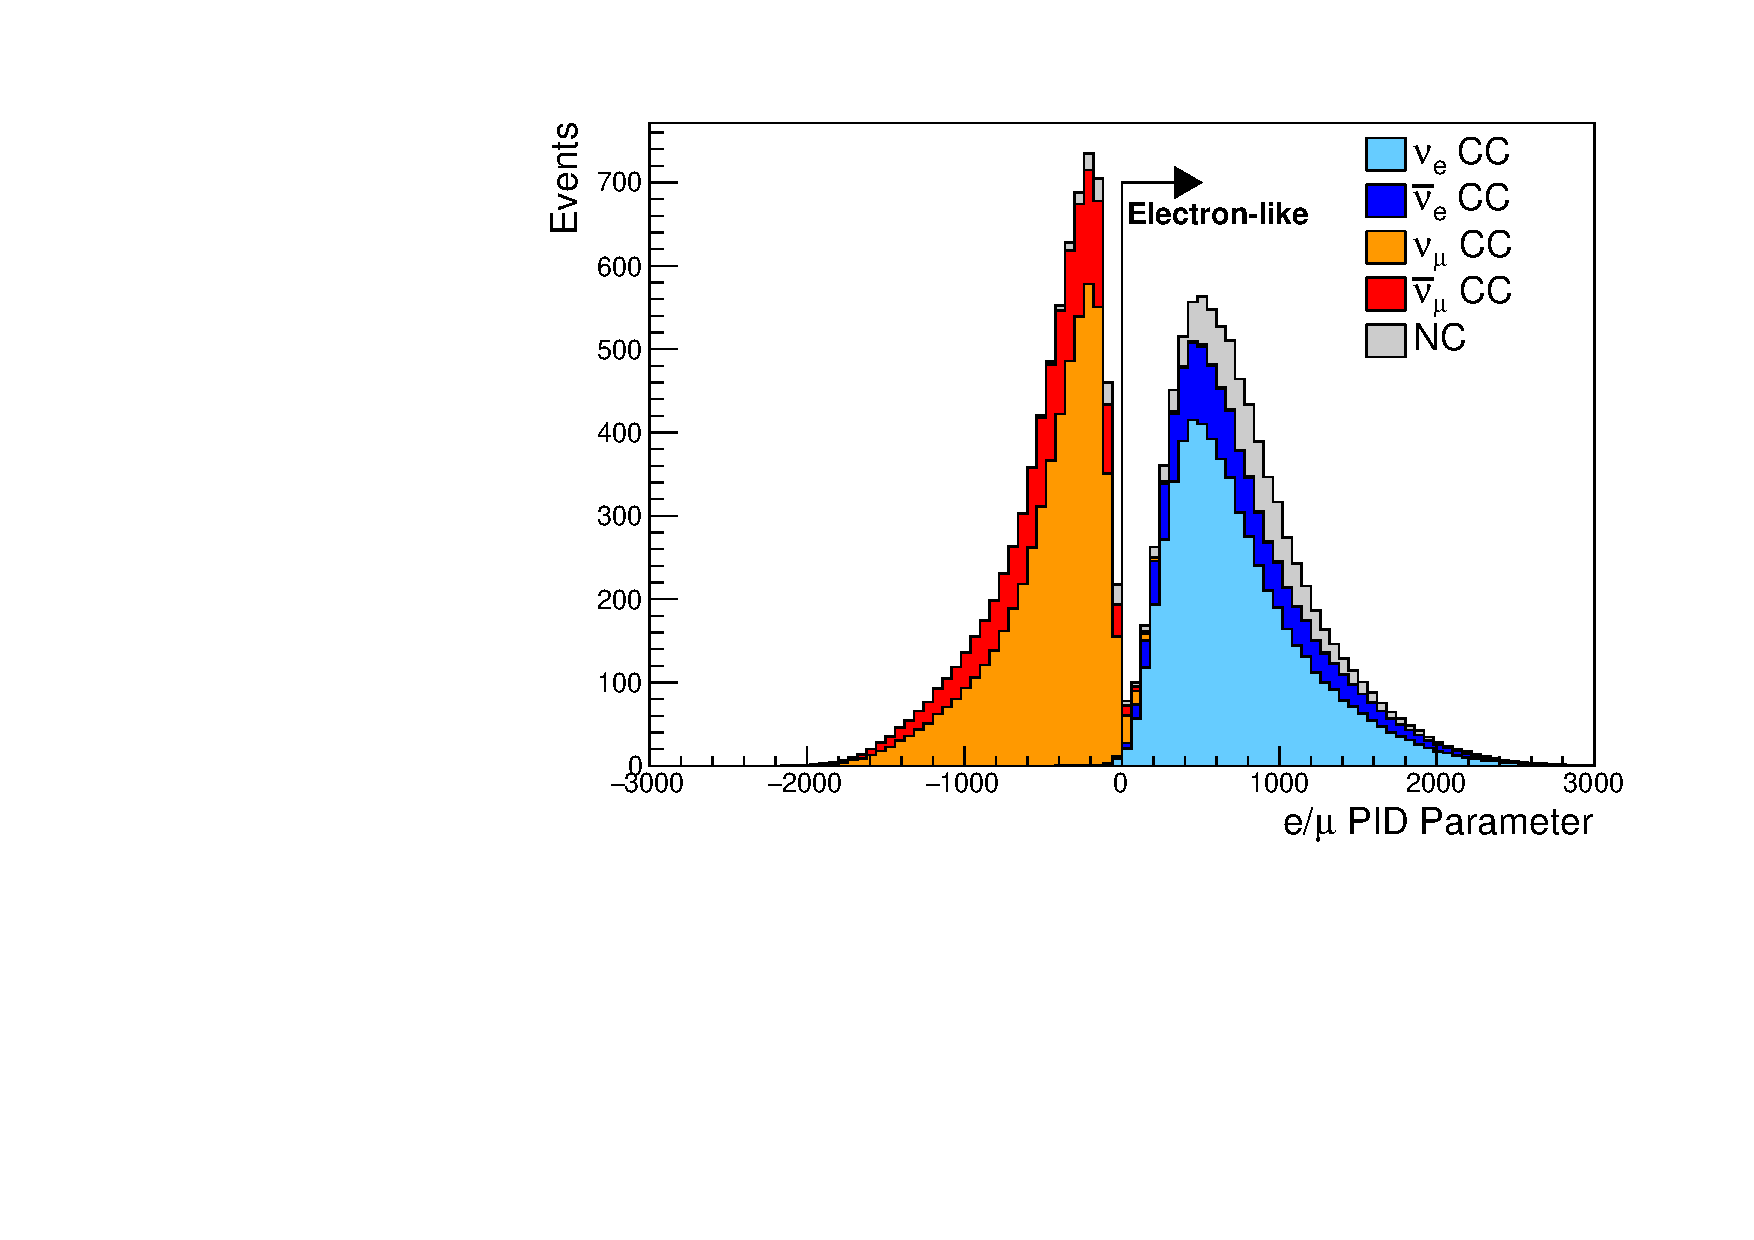
\includegraphics[width=\textwidth, trim={0mm 0mm 0mm 0mm}, clip, page=1]{Figures/Simulations/PIDParameter.pdf}
  \end{subfigure}
  \caption{The electron/muon PID separation parameter for all sub-GeV single-ring events in SK-IV. The charged current (CC) component is broken down in four flavours of neutrino (\quickmath{\nu_{\mu}}, \quickmath{\bar{\nu}_{\mu}}, \quickmath{\nu_{e}} and \quickmath{\bar{\nu}_{e}}). Events with positive values of the parameter are determined to be electron-like.}
  \label{fig:Simulations_EMUPIDParamDistribution}
\end{figure}

The \fq algorithm also considers a \quickmath{\pi^{0}} hypothesis. To do this, it performs a fit looking for two standard electron-hypothesis tracks which point to the same four-vertex. This assumes the electron tracks are generated from photon-conversion so the electron tracks actually appear offset from the proposed \quickmath{\pi^{0}} vertex. For these fits, the conversion length, direction, and momenta of each photon are also considered as track parameters which are then fit in the same methodology as the standard single-ring hypotheses. 

Whilst low energy events are predominately single-ring events, higher energy neutrino events can generate finals states with multiple particles which generate Cherenkov photons. These ``multi-ring'' hypotheses are also considered in the \fq algorithm. When calculating the charge likelihood density, the predicted charge associated with each ring is calculated separately and then merged to calculate the total accumulated charge on each PMT. Similarly, the time likelihood for the multi-ring hypothesis is calculated assuming each ring is independent. Each track is time-ordered based on the time of flight from the center of the track to the PMT and the direct light from any ring incident on the PMT is assumed to arrive before any scattered light. To reduce computational resources, the multi-ring fits only consider electron-like and charged pion-like rings as the pion fit can be used as a proxy for a muon fit due to their similar mass.

Multi-ring fits proceed by proposing another ring to the previous fit and then fitting the parameters in the method described above. Typically, multi-ring fits have the largest likelihood because of the additional degrees of freedom introduced. Consequently, the additional ring is only added if the ratio of likelihoods passes a criterion, which is determined by Monte Carlo studies.

As an example of how the reconstruction depends on the detector conditions, the author of this thesis assessed the quality of event reconstruction for SK-V data. The detector systematics invoked within the T2K-only oscillation analysis are determined using data to Monte Carlo comparisons using the SK-IV data \cite{t2k_tn_326}. Due to tank-open maintenance occurring between SK-IV and SK-V, the dark rate of each PMT was observed to increase in SK-V due to light exposure for a significant time during the repairs. This increase can be seen in \autoref{fig:Simulations_DarkRateVariation}. Run-10 of the T2K experiment was conducted in the SK-V period, so the consistency of SK-IV and SK-V data needs to be studied to determine whether the SK-IV-defined systematics can be applied to the run-10 data. This comparison study was performed using the stopping muon data set for both the SK-IV and SK-V periods. This data sample is used due to the high rate of interactions (\quickmath{O(200)} events per hour) as well as having similar energies to muons from CCQE \quickmath{\nu_{\mu}} interactions from beam interactions. The rate of cosmic muons does depend on the solar activity cycle \cite{Maghrabi2021} but has been neglected in this comparison study. This is because the shape of the distributions is most important for the purposes of being compared to the detector systematics. The SK-IV and SK-V data samples consist of \quickmath{2398.42} and \quickmath{626.719} hours of data which equates to \quickmath{686\text{k}} and \quickmath{192\text{k}} events respectively.

\begin{figure}[h]
  \begin{subfigure}[t]{\textwidth}
    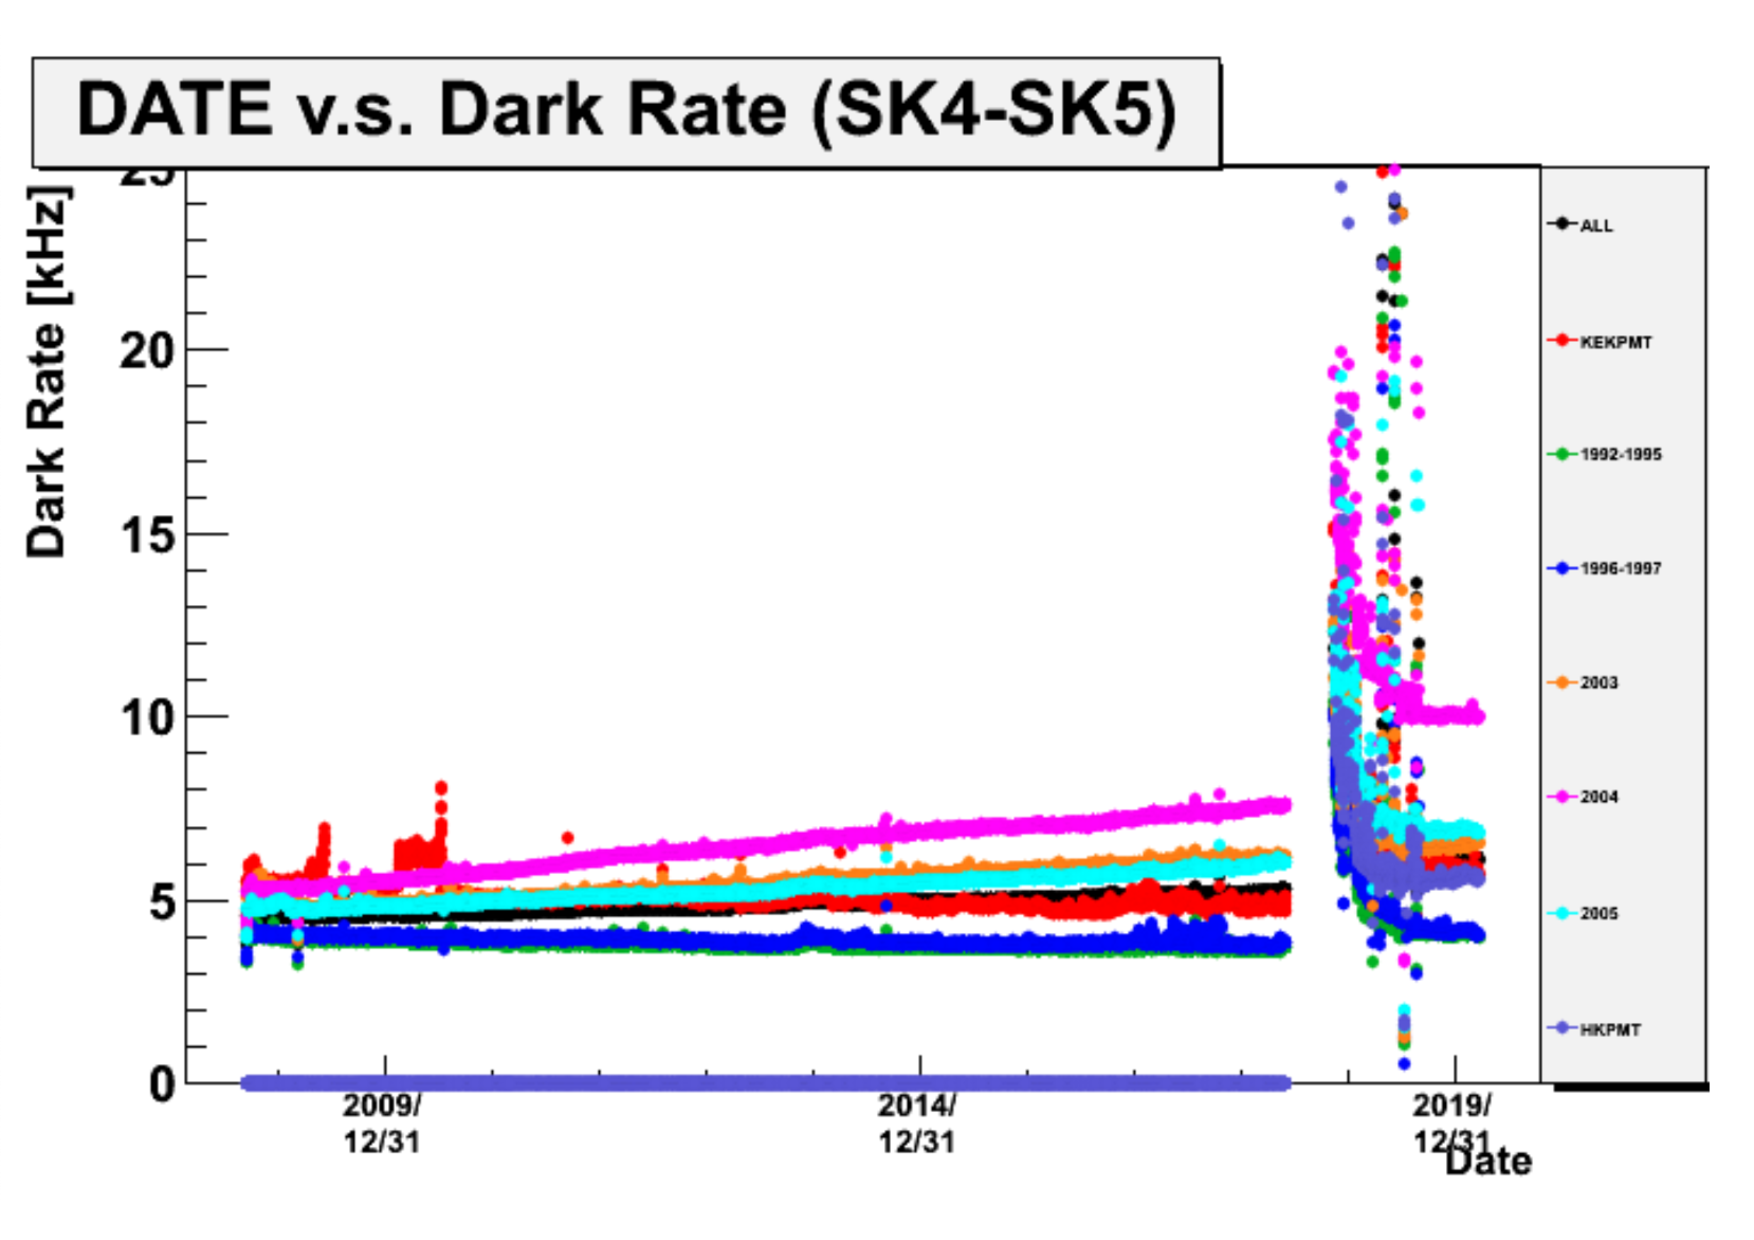
\includegraphics[width=\textwidth, trim={0mm 0mm 0mm 0mm}, clip, page=1]{Figures/Simulations/DarkRate.pdf}
  \end{subfigure}
  \caption{The variation of the measured dark rate as a function of date, broken down by PMT type. The SK-IV and SK-V periods span September 2008 to May 2018 and January 2019 to July 2020, respectively. The break in measurement in 2018 corresponds to the period of tank repair and refurbishment. Figure adapted from \cite{t2k_tn_326}.}
  \label{fig:Simulations_DarkRateVariation}
\end{figure}

The predicted charge calculated in the \fq charge likelihood prediction includes a contribution from the photoelectron emission due to dark noise. Therefore, the increase in the SK-V dark rate needs to be accounted for. In practice, the average dark rate in each SK period is calculated and used as an input in the reconstruction. This is calculated by averaging the dark rate per run for each period separately, using the calibration measurements detailed in \autoref{subsec:T2KSKExp_SKCalibration}. The average dark rate from SK-IV and SK-V were found to be \quickmath{4.57\text{kHz}} and \quickmath{6.30\text{kHz}}, respectively. The associated charge with the muon and decay electron subevents are illustrated in \autoref{fig:Simulations_MeasuredChargeDistribution}. The photoelectron emission from dark noise will be more noticeable for events that have lower energy. This is because this contribution becomes more comparable to the number of photoelectrons emitted from incident photons in low-energy events. This behaviour is observed in the data, where the charge deposited by the muon subevent is mostly unaffected by the increase in dark rate, whilst the charge associated with the decay-electron is clearly affected.

\begin{figure}[h]
  \begin{subfigure}[t]{0.48\textwidth}
    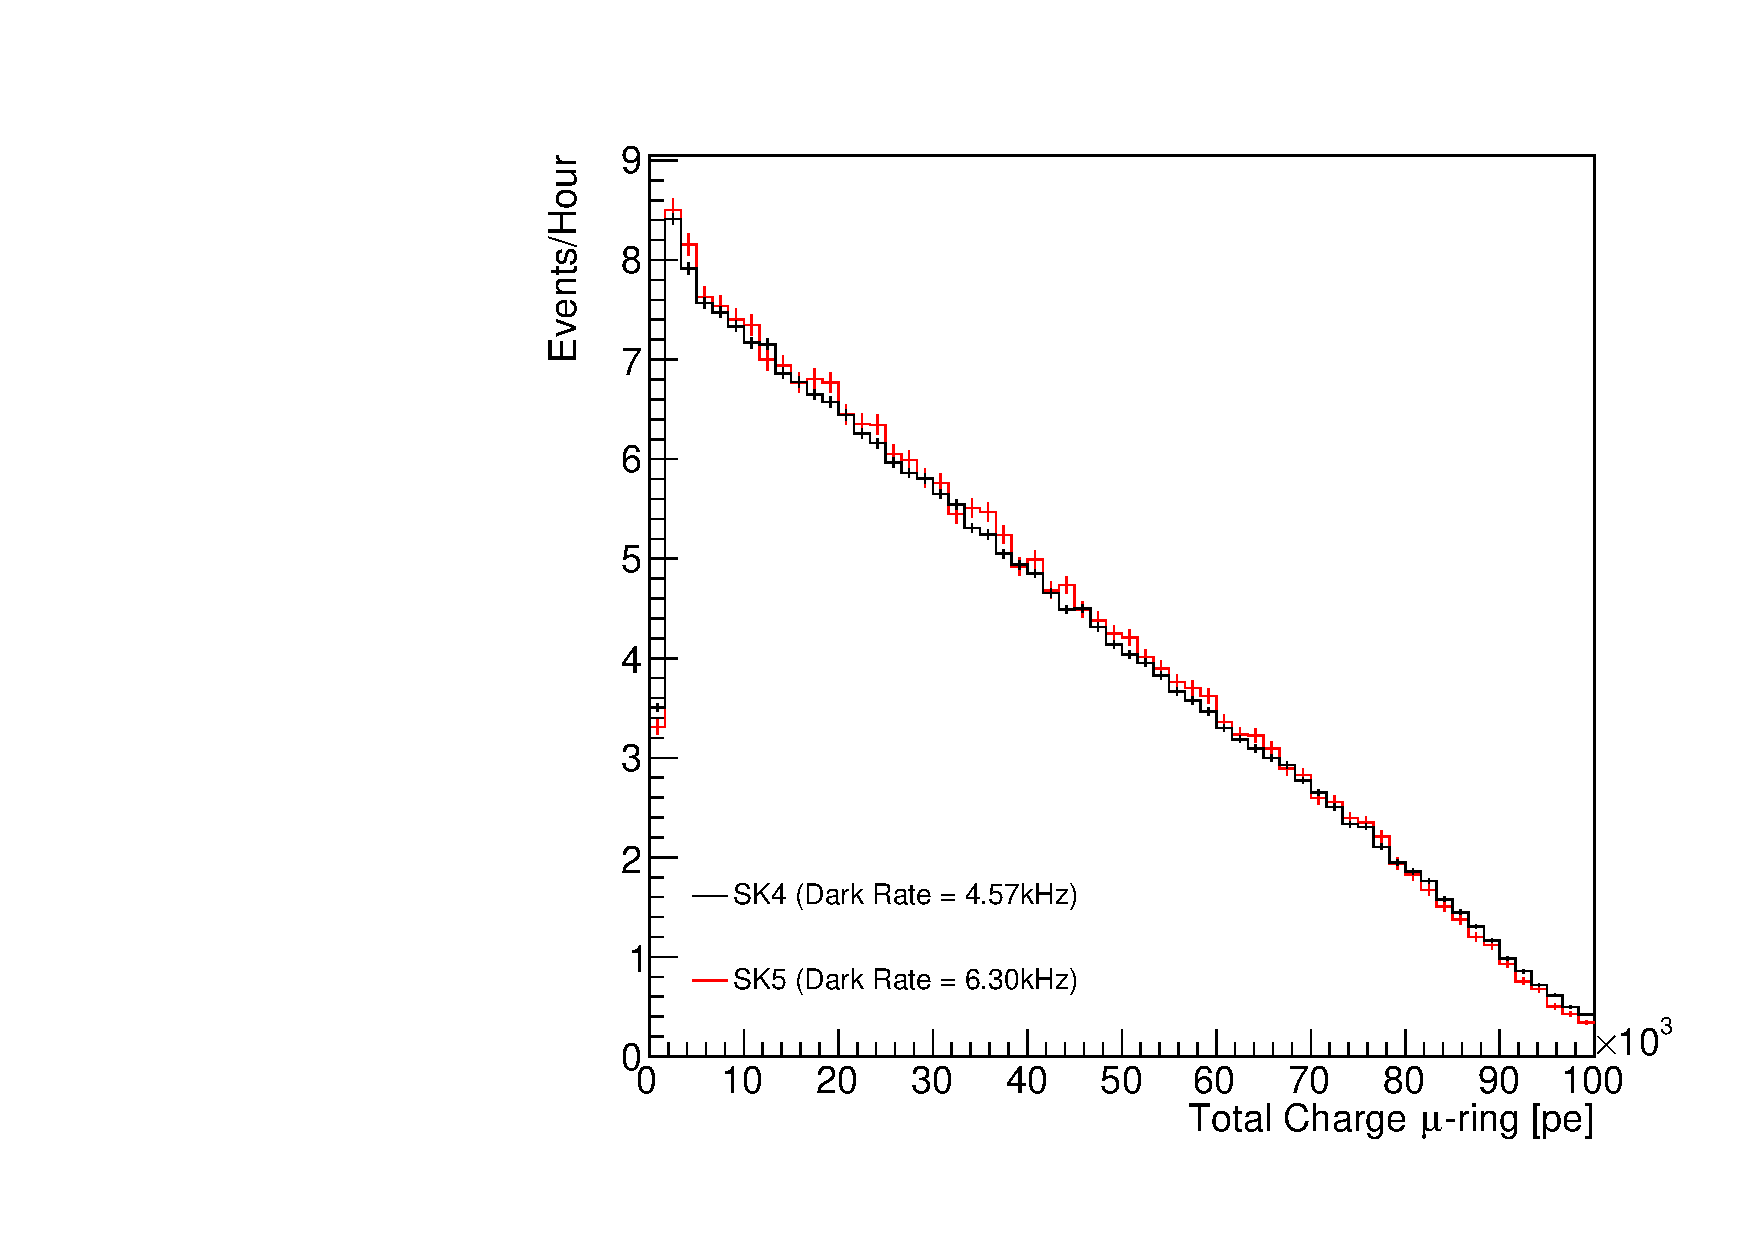
\includegraphics[width=\textwidth, trim={0mm 0mm 0mm 0mm}, clip, page=1]{Figures/Simulations/ChargeAssociatedWithMuon.pdf}
    \subcaption{Muon}
  \end{subfigure}%
  \begin{subfigure}[t]{0.48\textwidth}
    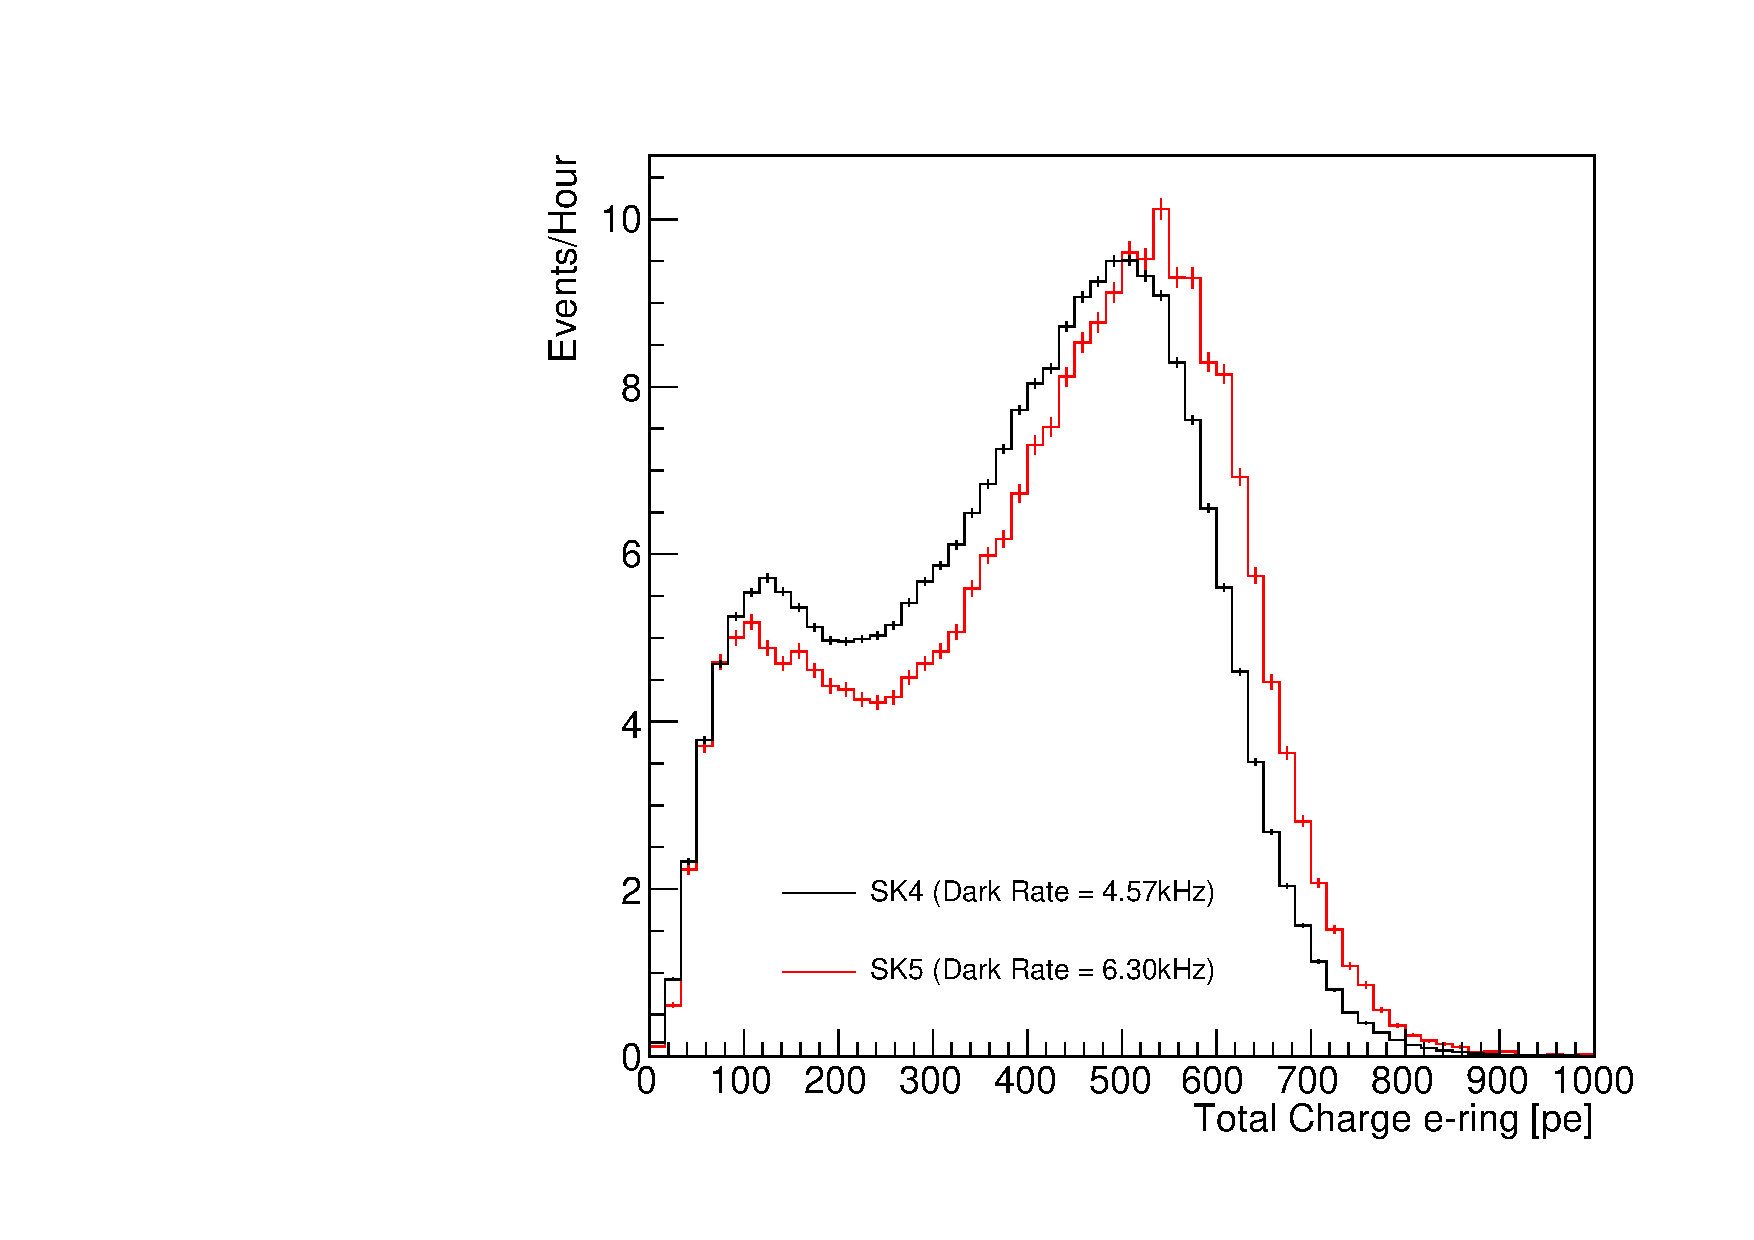
\includegraphics[width=\textwidth, trim={0mm 0mm 0mm 0mm}, clip, page=1]{Figures/Simulations/ChargeAssociatedWithDecayE.pdf}
    \subcaption{Decay Electron}
  \end{subfigure}  
  \caption{Comparison of the measured raw charge deposited per event from the stopping muon data samples between SK-IV (Blue) and SK-V (Red), split by the primary muon subevent and the associated decay electron subevent.}
  \label{fig:Simulations_MeasuredChargeDistribution}
\end{figure}

The energy scale systematic for the SK-IV period was determined to be \quickmath{2.1\%} \cite{sk_2017}. It is defined to be equal to the difference between data and Monte Carlo prediction in the stopping muon data sample. To determine the consistency of the SK-IV and SK-V with respect to the energy scale systematic, the muon momentum distribution is compared between the two SK periods. As the total number of Cherenkov photons is integrated across the track length, the reconstructed momentum divided by track length (or range) is compared between SK-IV and SK-V as illustrated in \autoref{fig:Simulations_MuonMomentumByRange}.

\begin{figure}[h]
  \begin{subfigure}[t]{\textwidth}
    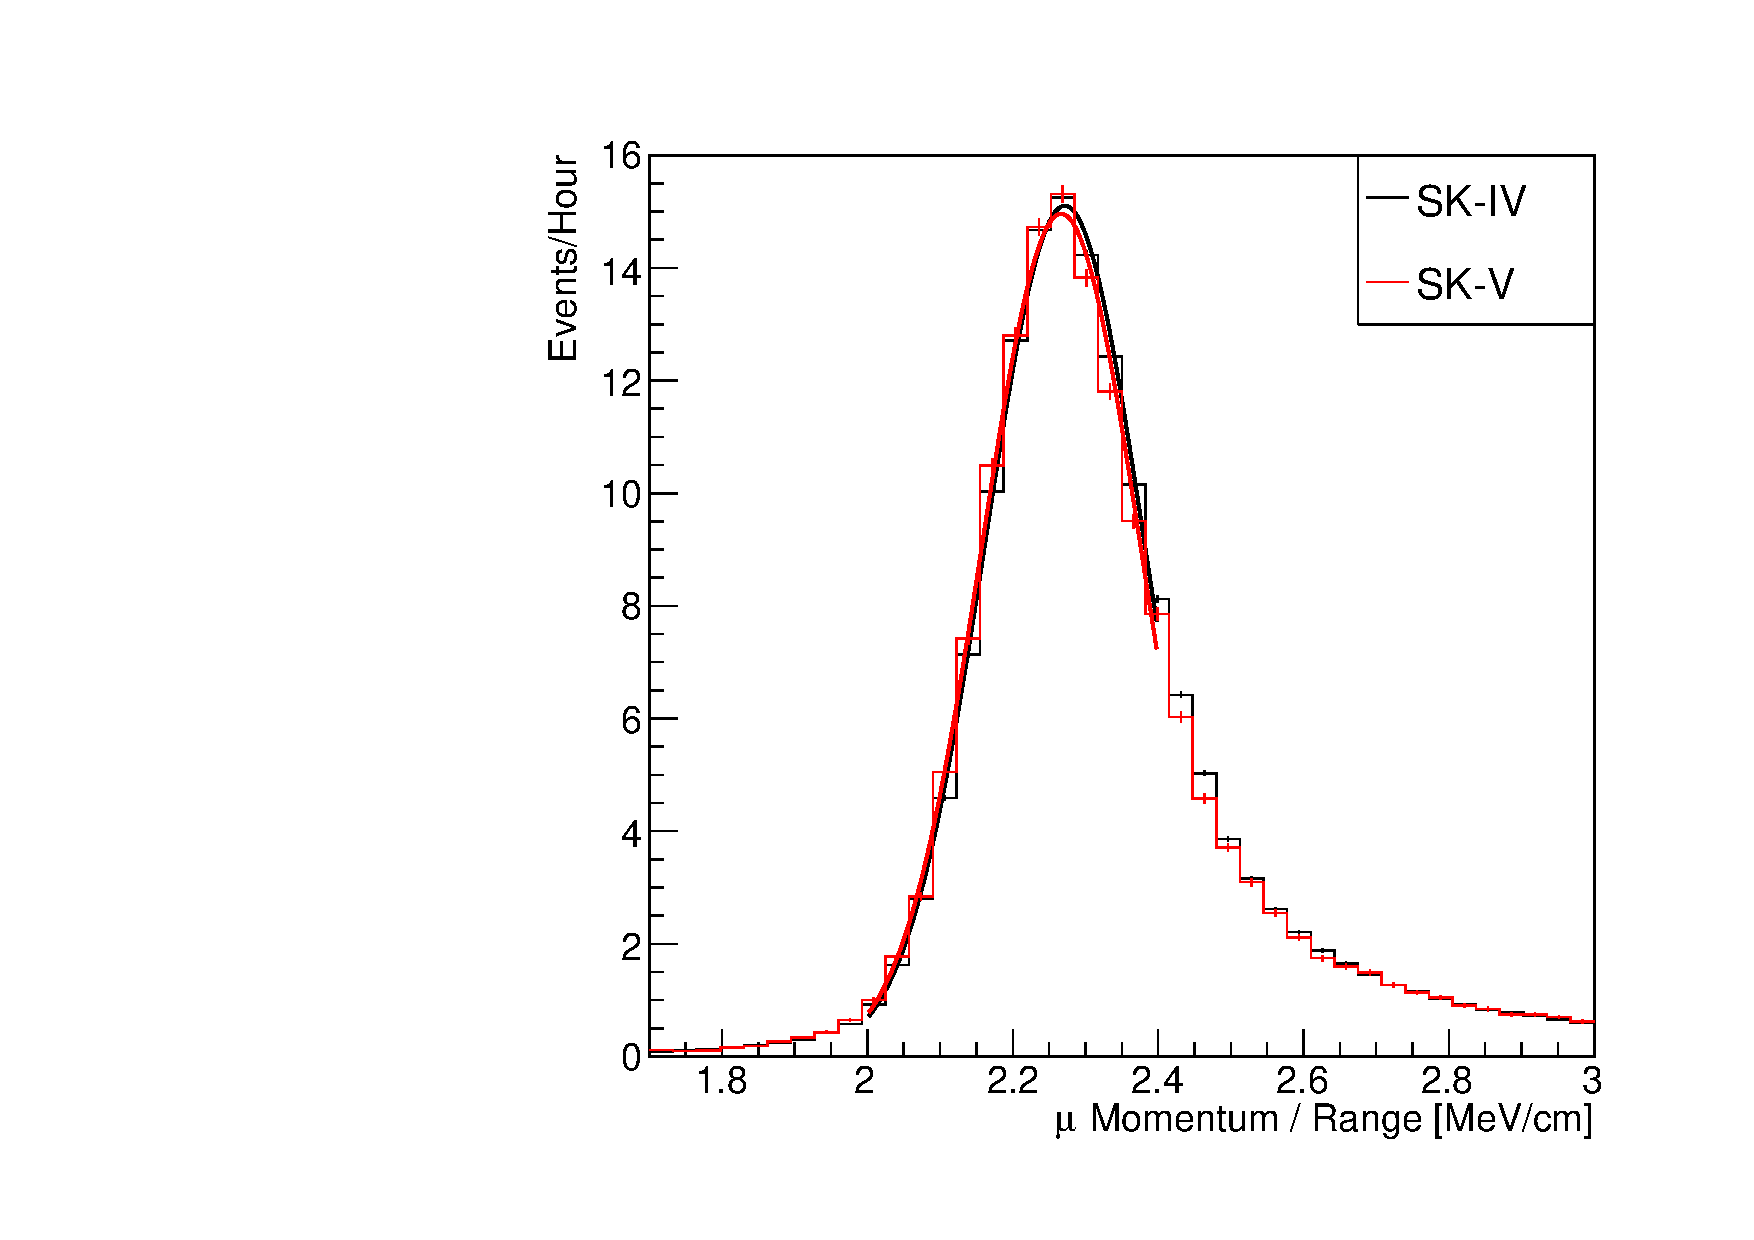
\includegraphics[width=\textwidth, trim={0mm 0mm 0mm 0mm}, clip, page=1]{Figures/Simulations/MuonRangeComparison.pdf}
  \end{subfigure}
  \caption{The distribution of the reconstructed momentum from the muon ring divided by the distance between the reconstructed muon and decay electron vertices as found in the stopping muon data sets of SK-IV (Black) and SK-IV (Red). Only events with one tagged decay electron are considered. A Gaussian fit is considered in the range \quickmath{[2.0,2.4] \text{MeV/cm}} and illustrated as the solid curve.}
  \label{fig:Simulations_MuonMomentumByRange}
\end{figure}

The consistency between these distributions has been computed in two ways. Firstly, a Gaussian is fit to each distribution separately. The mean of which is found to be \quickmath{(2.272 \pm 0.003) \text{MeV/cm}} and \quickmath{(2.267 \pm 0.006) \text{MeV/cm}} for SK-IV and SK-V respectively. The ratio of these is equal to \quickmath{1.002 \pm 0.003}. The mean of the Gaussian fits are consistent with the expected stopping power of a minimum ionising muon for a target material (water) with \quickmath{Z/A \sim 0.5} \cite{PhysRevD.86.010001}. The second consistency check is performed by introducing a nuisance parameter, \quickmath{\alpha}, which modifies the SK-V distribution. The value of \quickmath{\alpha} which minimises the \quickmath{\chi^{2}} value between the SK-IV and SK-V is determined by scanning across a range of values. This is repeated by applying the nuisance parameter as both a multiplicative factor and an additive shift. The \quickmath{\chi^{2}} distributions for different values of \quickmath{\alpha} is illustrated in \autoref{fig:Simulations_MuonMomentumByRangeChi2Scan}. The values which minimise the \quickmath{\chi^{2}} are found to be \quickmath{0.0052} and \quickmath{1.0024} for the additive and multiplicative implementations, respectively. No evidence of shifts larger than the \quickmath{2.1\%} uncertainty on the energy scale systematic has been found in the reconstructed momentum distribution of SK-IV and SK-V.

\begin{figure}[h]
  \begin{subfigure}[t]{\textwidth}
    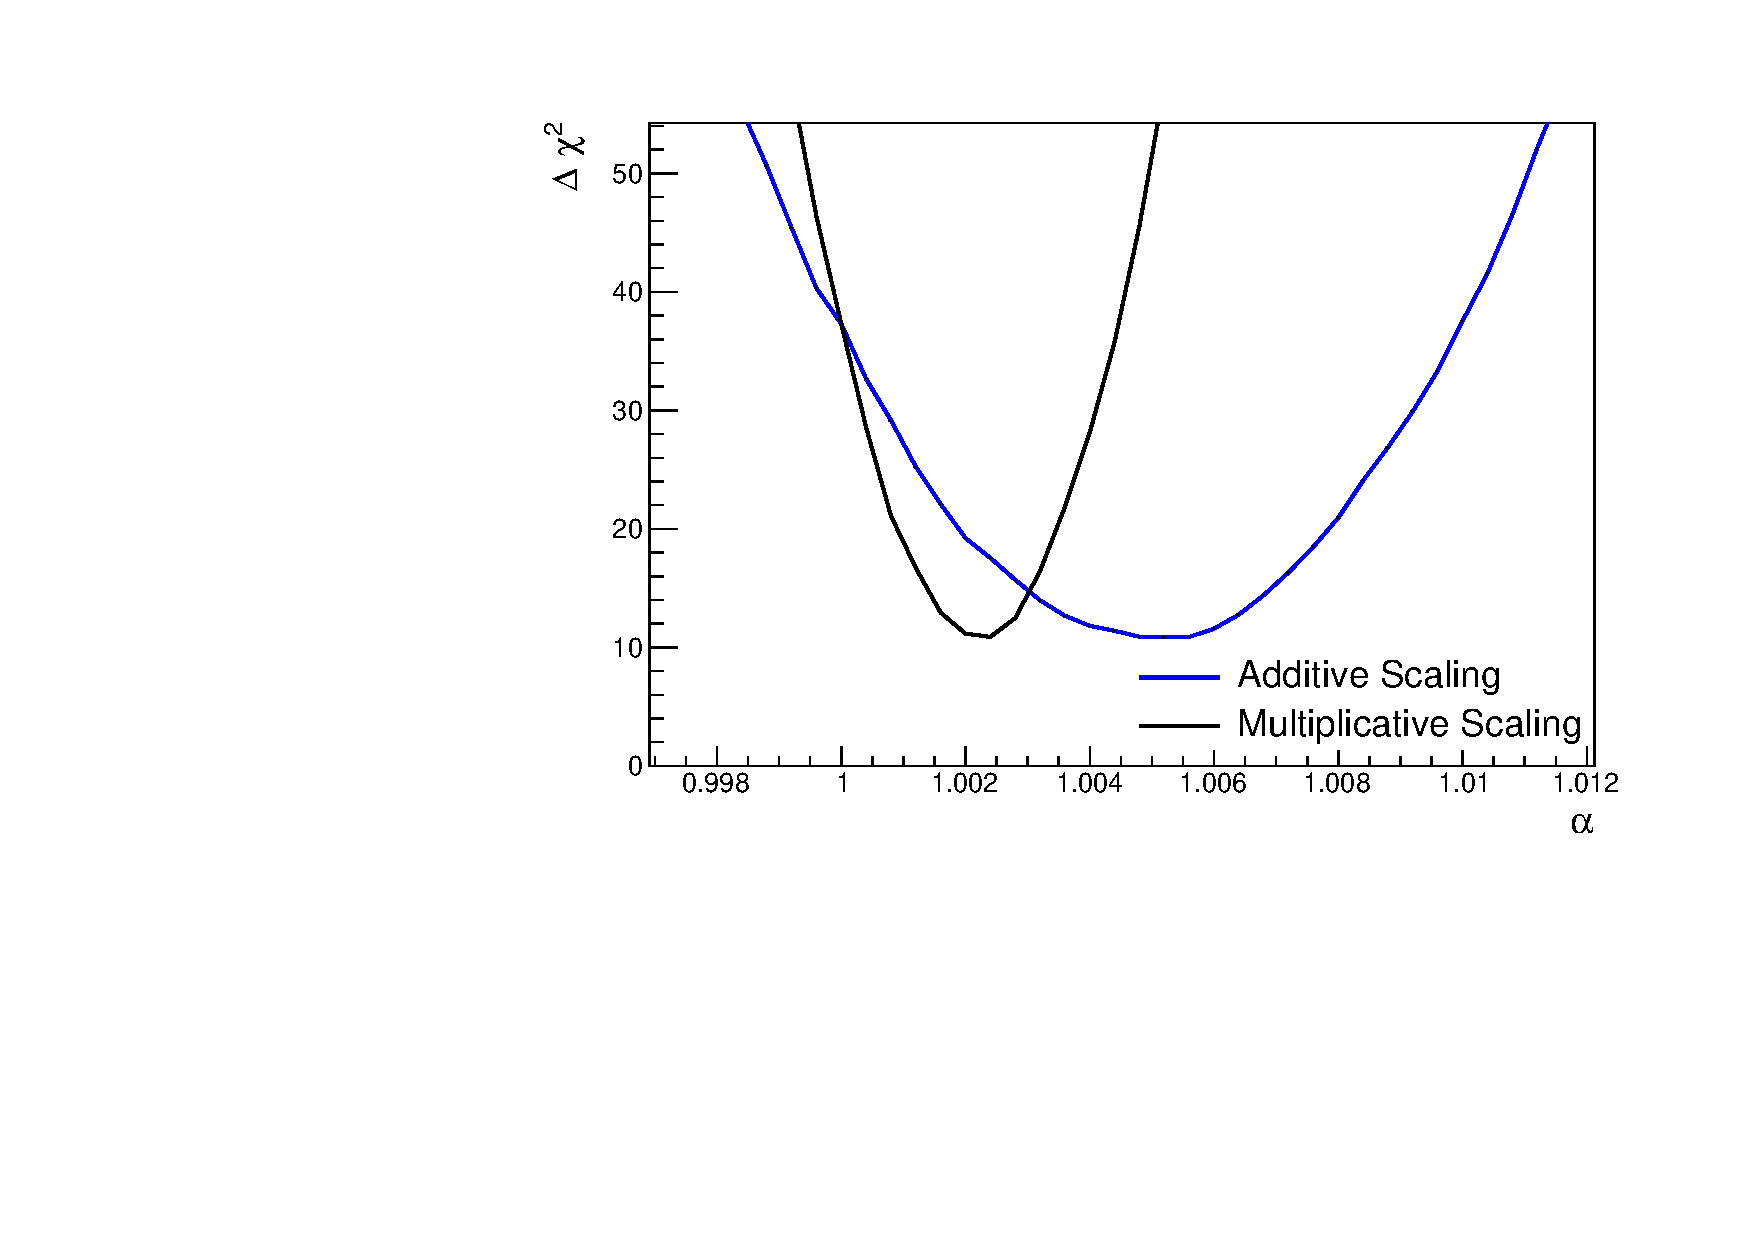
\includegraphics[width=\textwidth, trim={0mm 0mm 0mm 0mm}, clip, page=1]{Figures/Simulations/MuonRange_Chi2Scan.pdf}
  \end{subfigure}
  \caption{The \quickmath{\chi^{2}} difference between the SK-IV and SK-V reconstructed muon momentum divided by range when the SK-V is modified by the scaling parameter \quickmath{\alpha}. Both additive (Blue) and multiplicative (Black) scaling factors have been considered. In practice, the additive scaling factor actually uses the value of (\quickmath{\alpha-1.0}) but is illustrated like this so the results can be shown on the same axis range.}
  \label{fig:Simulations_MuonMomentumByRangeChi2Scan}
\end{figure}

\section{Event Reduction at SK}
\label{sec:Simulations_Reduction}

Atmospheric neutrino events observed in the SK detector are categorised into three different types of samples: fully contained (FC), partially contained (PC) and up-going muon (Up-$\mu$), using PMT hit signatures in the inner and outer detector (ID and OD, respectively). To identify FC neutrino events, it is required that the neutrino interacts inside the fiducial volume of the ID such that no significant OD activity is observed. For this analysis, an event is defined to be in the fiducial volume providing the event vertex is at least $0.5$m away from the ID walls. PC events have the same ID requirements but can have a larger signal present inside the OD. Typically these events are higher energy muon interactions that penetrate the ID walls. The Up-$\mu$ sample contains events where muons are created from neutrino interactions in the OD water or rock below the tank. They then propagate upwards through the detector. The reason downward-going muons generated from neutrino interactions above the tank are neglected is due to the difficulty in separating their signature from the cosmic muon shower background. The sample categories are visually depicted in Figure \ref{fig:Simulations_AtmosphericSampleTopology}.

\begin{figure}[ht!]
    \centering
    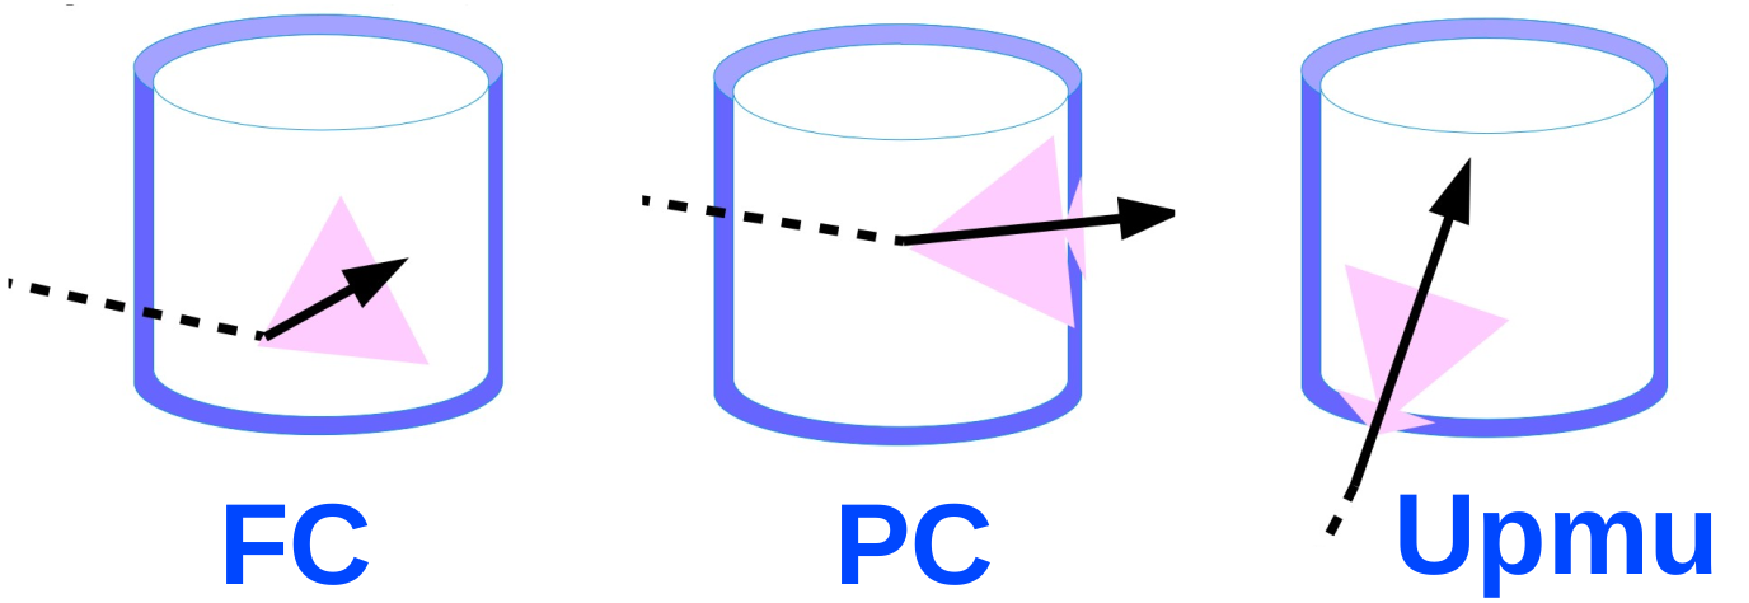
\includegraphics[width=0.8\textwidth]{Figures/Simulations/Atmo_topology.pdf}
    \caption{A depiction of the topology patterns for fully-contained (FC), partially-contained (PC) and up-going muon (\quickmath{\text{Up-}\mu}) samples included in this analysis.}
    \label{fig:Simulations_AtmosphericSampleTopology}
\end{figure}

Based on the event characteristics, as defined by the \fq event reconstruction software, the FC events are categorised by

\begin{itemize}
    \item \textbf{Visible Energy}: equal to the sum of the reconstructed kinetic energy above the Cerenkov threshold for all rings present in the event. The purpose is to separate events into sub-GeV and multi-GeV categories. 
    \item \textbf{Number of observed Cerenkov rings}. The purpose is to separate single-ring and multi-ring events, where single-ring events predominantly consist of quasi-elastic interactions and multi-ring events are typically resonant pion production or deep inelastic scattering events.
    \item \textbf{Particle identification parameter of the most energetic ring}: A value determined from the maximum likelihood value based on \texttt{fiTQun}'s electron, muon, or pion hypothesis. The purpose is to separate electron-like and muon-like events.
    \item \textbf{Number of decay electrons}: The purpose is to separate quasi-elastic events (which have one decay electron emitted from the muon decay) and resonant pion production events (which have two decay electrons emitted from the muon and pion).
\end{itemize}

The PC and \quickmath{\text{Up-}\mu} categories are broken down into ``through-going'' and ``stopping'' samples depending on whether the muon left the detector. This is because the stopping events deposit the entire energy of the interaction into the detector, resulting in better reconstruction. The energy of events that exit the detector has to be estimated which introduces much larger systematic uncertainties. Through-going \quickmath{\text{Up-}\mu} samples are further broken down by whether any hadronic showering was observed in the event which typically indicates DIS interactions. The expected neutrino energy for the different categories is given in \autoref{fig:Simulations_NeutrinoEnergyDistribution}. FC sub-GeV and multi-GeV events peak around \quickmath{0.7\text{GeV}} and \quickmath{3\text{GeV}} respectively, with slightly different peak energies for \quickmath{\nu_{x} \rightarrow \nu_{e}} and \quickmath{\nu_{x} \rightarrow \nu_{\mu}} oscillation channels. PC and \quickmath{\text{Up-}\mu} are almost entirely comprised of \quickmath{\nu_{x} \rightarrow \nu_{\mu}} events and peak around \quickmath{7\text{GeV}} and \quickmath{100\text{GeV}}, respectively.

\begin{figure}[h]
  \begin{subfigure}[t]{0.49\textwidth}
    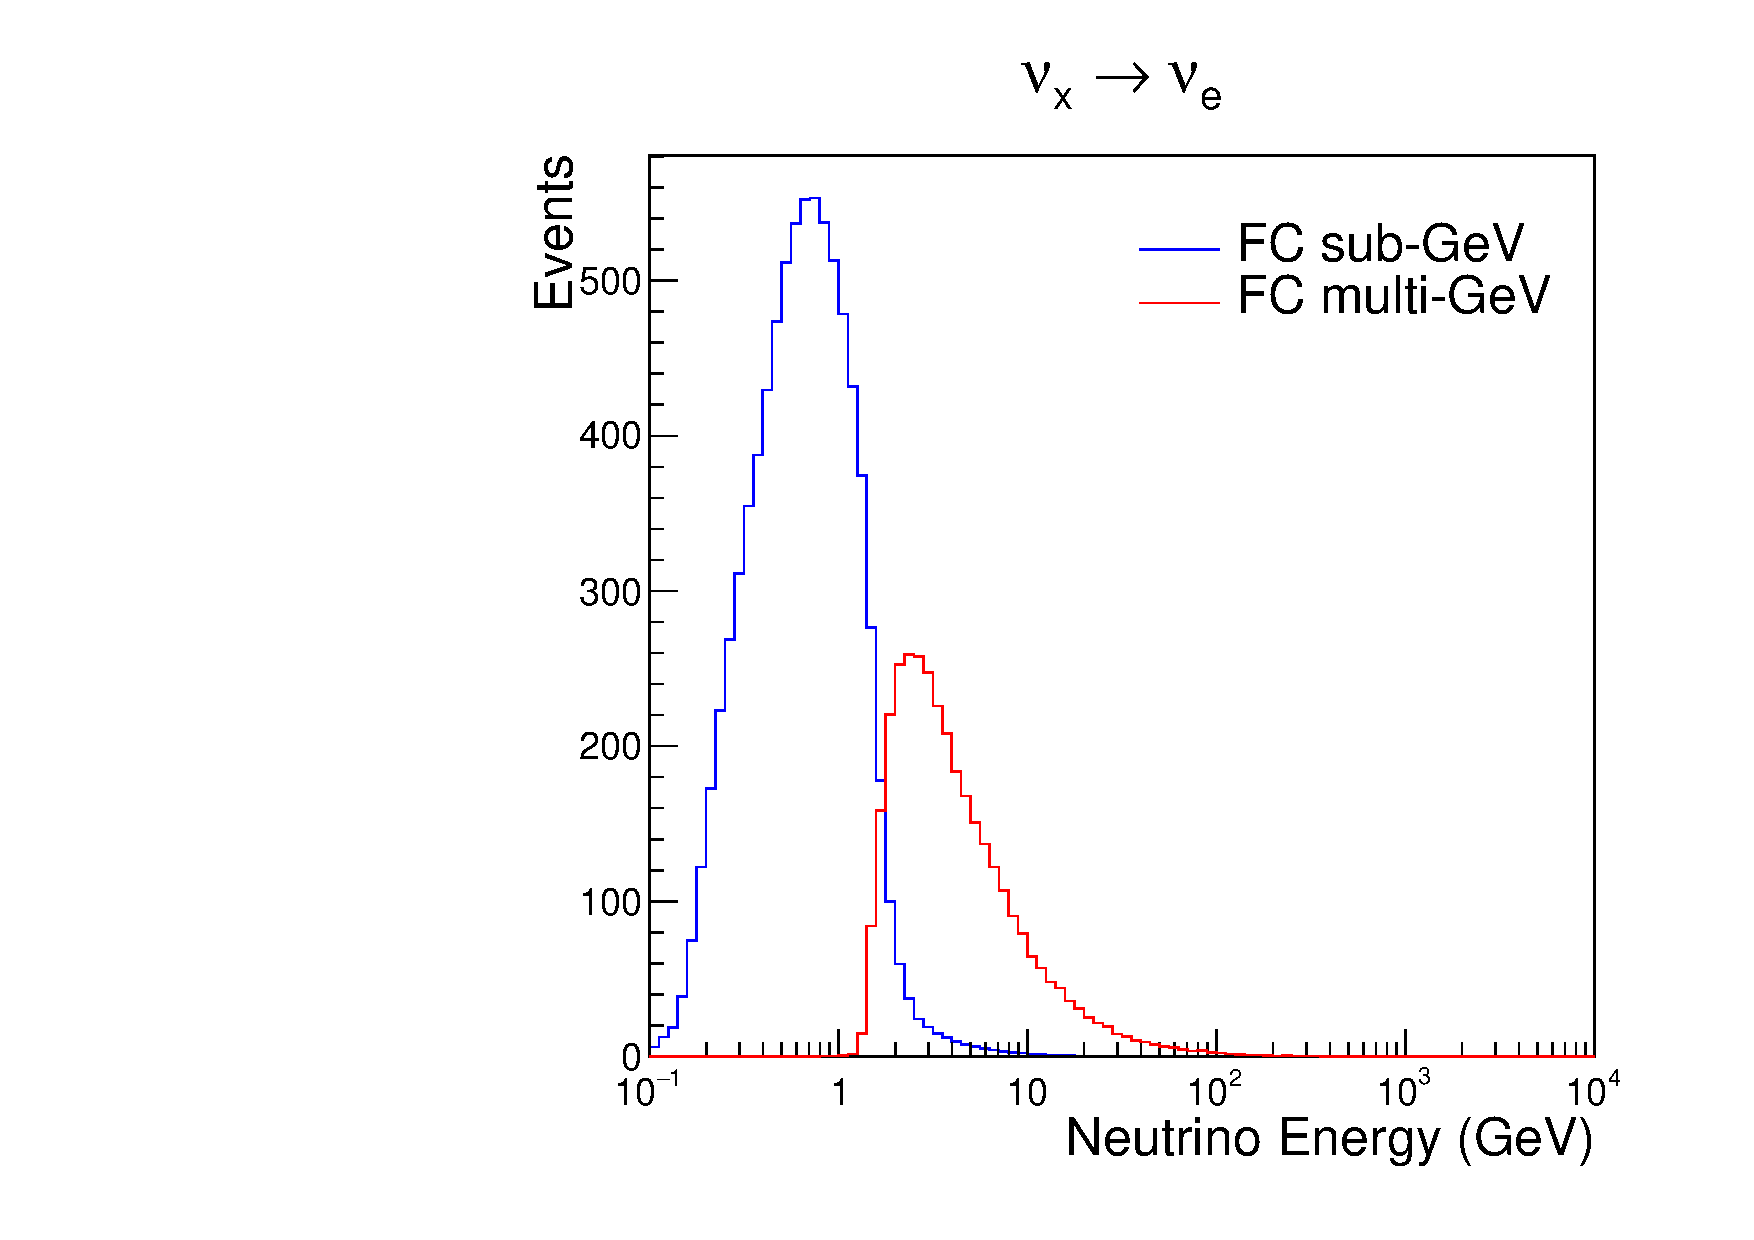
\includegraphics[width=\textwidth, trim={0mm 0mm 0mm 0mm}, clip,page=1]{Figures/Simulations/NeutrinoEnergyDist_NuE.pdf}
  \end{subfigure}%
  \begin{subfigure}[t]{0.49\textwidth}
    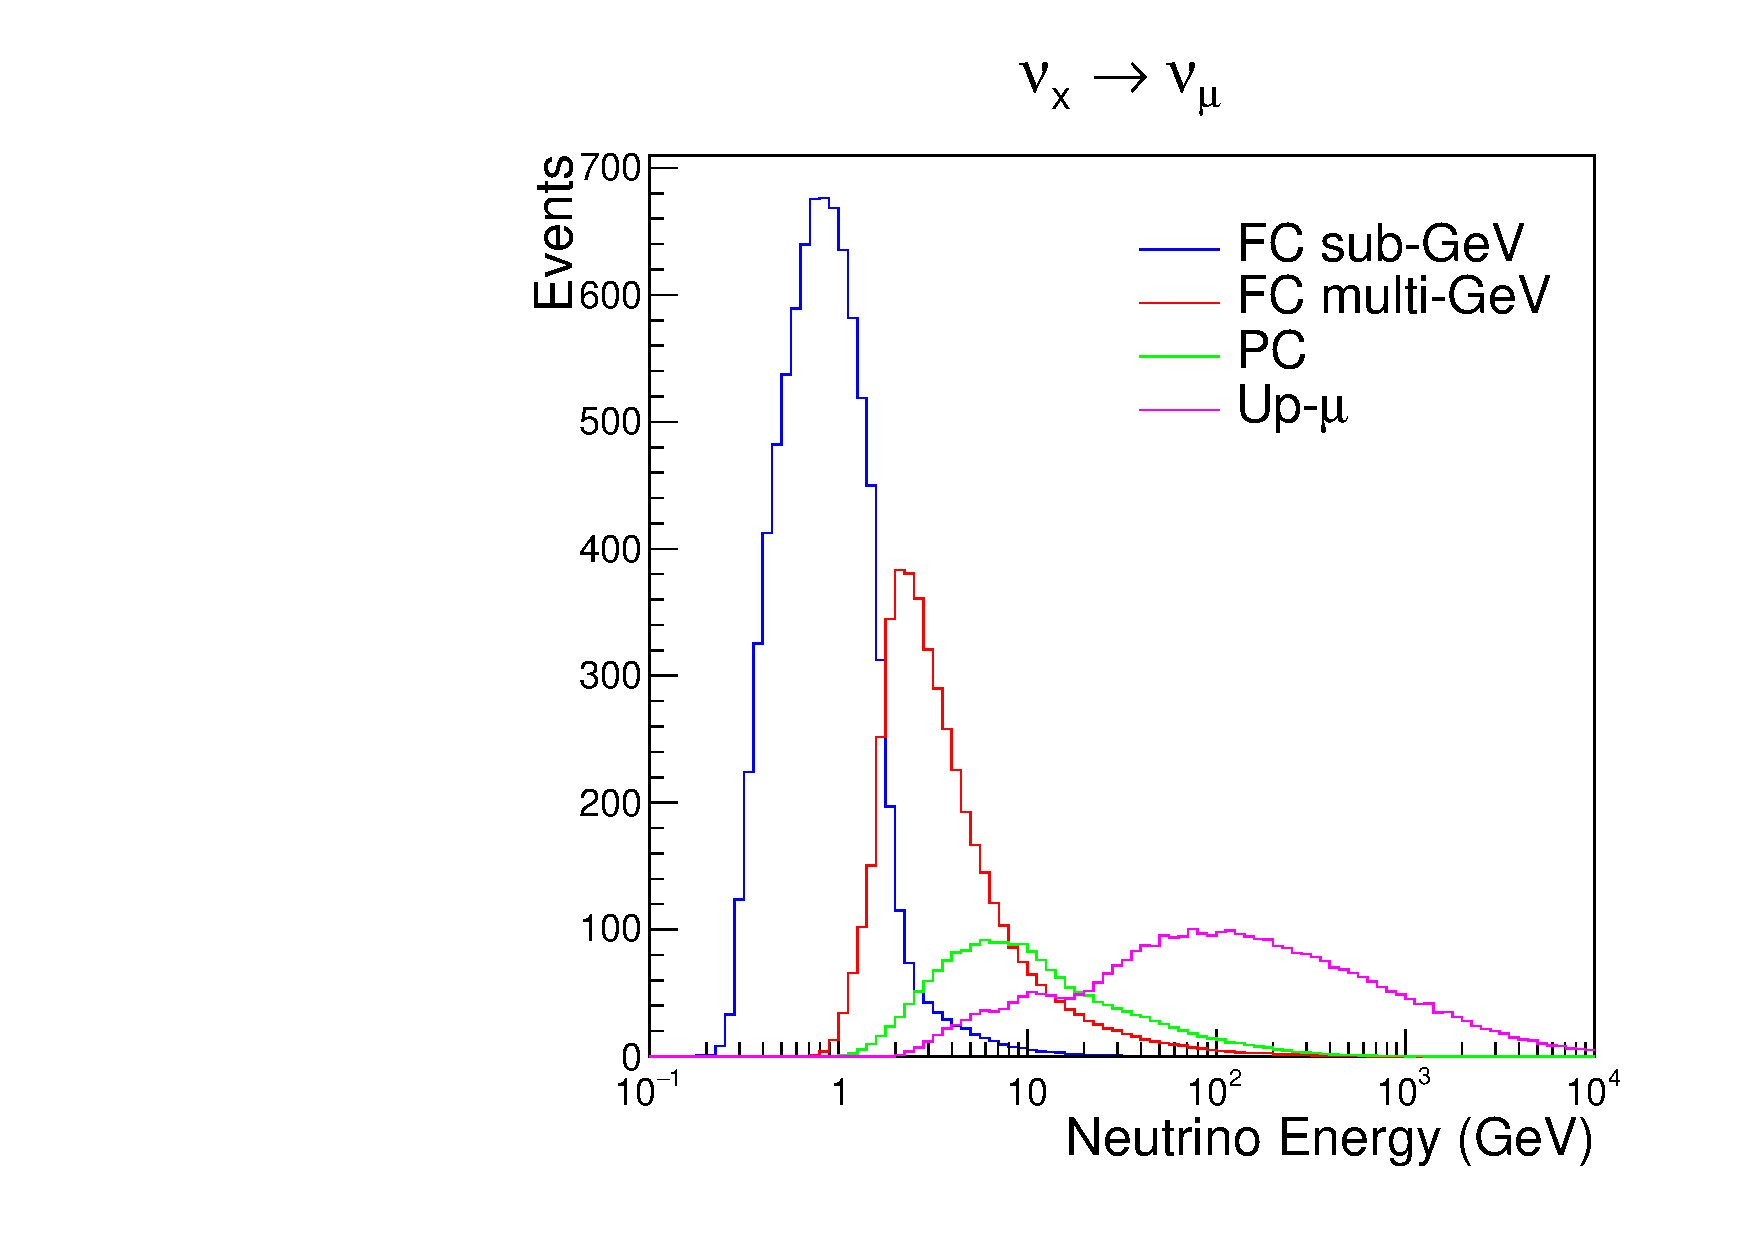
\includegraphics[width=\textwidth, trim={0mm 0mm 0mm 0mm}, clip,page=1]{Figures/Simulations/NeutrinoEnergyDist_NuMu.pdf}
  \end{subfigure}
  \begin{subfigure}[t]{0.49\textwidth}
    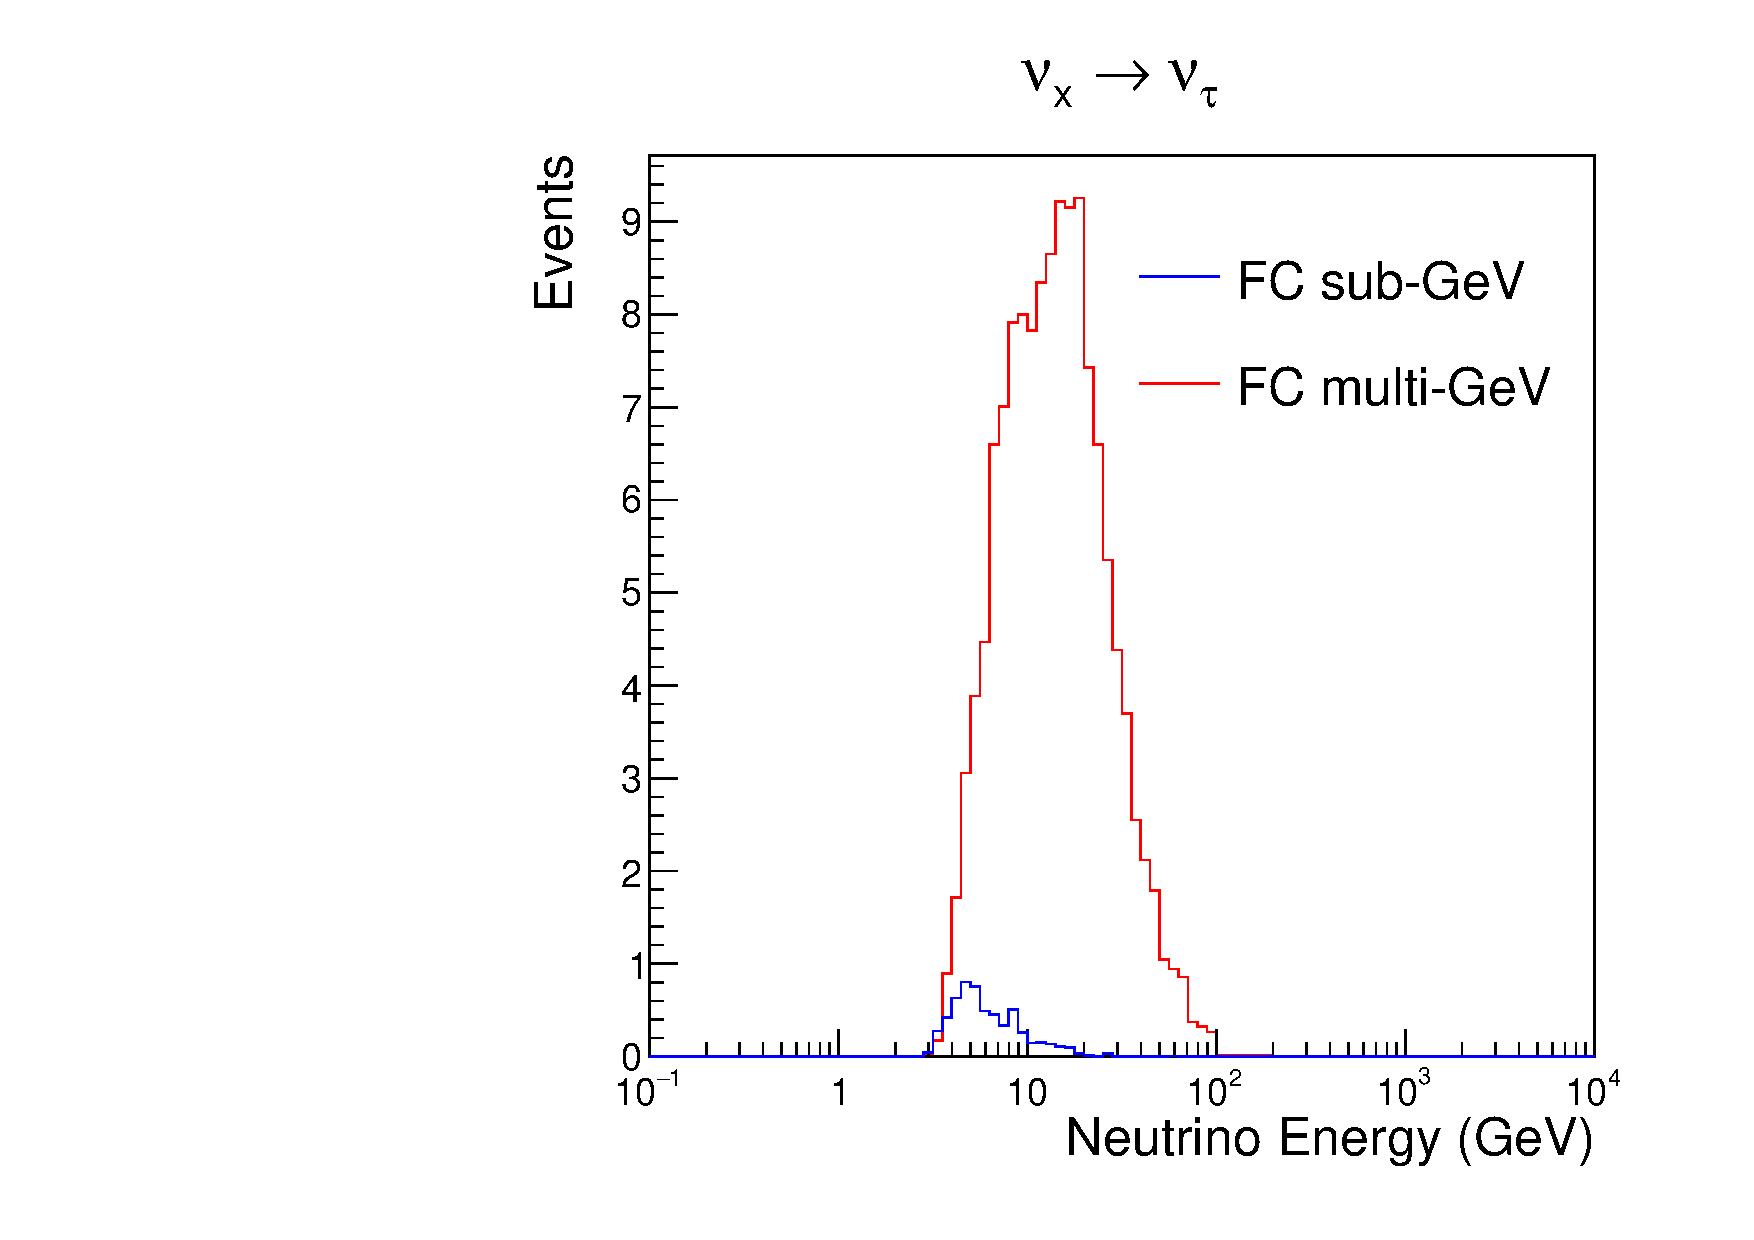
\includegraphics[width=\textwidth, trim={0mm 0mm 0mm 0mm}, clip,page=1]{Figures/Simulations/NeutrinoEnergyDist_NuTau.pdf}
  \end{subfigure}%
  \caption{The predicted neutrino flux of the fully contained (FC) sub-GeV and multi-GeV, partially contained (PC), and upward-going muon (\quickmath{\text{Up-}\mu}) events. The prediction is broken down by the \quickmath{\nu_{x} \rightarrow \nu_{e}} prediction (top left), \quickmath{\nu_{x} \rightarrow \nu_{\mu}} prediction (top right) and \quickmath{\nu_{x} \rightarrow \nu_{\tau}} prediction (bottom). All systematic dials are set to their nominal values and the Asimov A oscillation parameters are assumed.}
  \label{fig:Simulations_NeutrinoEnergyDistribution}
\end{figure}

In normal data-taking operations, the SK detector observes many background events alongside the beam and atmospheric neutrino signal events of physics interest. Cosmic ray muons and flasher events, which are the spontaneous discharge of a given PMT, contribute the largest amount of background events in the energy range relevant to any analysis searching for neutrino events. Lower energy analyses like DSNB searches are also subject to radioactive backgrounds \cite{Nakano_2017}. Therefore the data recorded is reduced with the aim of removing these background events. The reduction process is detailed in \cite{Ashie_2005, Jiang2019-iw} and briefly summarised below.

The first two steps in the FC reconstruction remove the majority of cosmic ray muons by requiring a significant amount of ID activity compared to that measured in the OD. Events that pass this cut are typically very high momentum muons or events that leave very little activity in the OD. Consequently, a third reduction step is then applied to select cosmic-ray muons that pass the initial reduction step. A purpose-built cosmic muon fitter is used to determine the entrance (or exit) position of the muon and a cut is applied to OD activity contained within \quickmath{8\text{m}} of this position. Flasher events are removed in the fourth reduction step which is based on the close proximity of PMT hits surrounding the PMT producing the flash. Events that pass all these reduction steps are reconstructed with the \apfit algorithm. The fifth step of the reduction uses information from the more precise fitter to repeat the previous two steps with tighter cuts. Muons below the Cherenkov threshold can not generate optical photons in the ID but the associated decay electron can due to its lower mass. These are the types of events targeted in the fifth reduction step. The final cuts require the event vertex to be within the fiducial volume (\quickmath{0.5\text{m}} from the wall although the nominal distance is \quickmath{2.0\text{m}}), visible energy \quickmath{E_{vis} > 30\text{MeV}} and fewer than 16 hits within the higher energy OD cluster. The culmination of the fully contained reduction results in \quickmath{8.09} events/day in the nominal fiducial volume \cite{thesis_miao}. The uncertainty in the reconstruction is calculated by comparing Monte Carlo prediction to data. The largest discrepancy is found to be \quickmath{1.3\%} in the fourth reduction step.

The PC and \quickmath{\text{Up-}\mu} events are processed through their own reduction processes detailed in \cite{Ashie_2005}. Both of these samples are reconstructed with the \apfit algorithm rather than \fq. This is because the efficiency of reconstructing events that leave the detector has not been sufficiently studied for reliable systematic uncertainties. The PC and \quickmath{\text{Up-}\mu} samples attain events at approximately \quickmath{0.66} and \quickmath{1.44} events/day.

Events due to beam neutrinos undergo the same reduction steps as FC events and are then subject to further cuts \cite{t2k_tn_027}. The GPS system which links the timing between the beam facility and SK needs to be operating correctly and there should be no activity within the detector in the previous \quickmath{100 \mu\text{s}} before the trigger. The events then need to triggered between \quickmath{-2 \mu\text{s}} and \quickmath{10\mu\text{s}} of the expected spill timing.

Due to the lower energy beam neutrinos, the T2K samples are not dependent upon the visible energy neutrino as the range of neutrino energies are smaller than that found in atmospheric neutrinos. Furthermore, the 2020 T2K-only oscillation analysis only considers events which contain a single ring. Similar to atmospheric event selection, the number of decay electrons is used as a proxy for distinguishing CCQE and CCRES events. The expected neutrino energy, broken down by number of decay electrons, is given in \autoref{fig:Simulations_NeutrinoEnergyDistribution_T2K}.

\begin{figure}[h]
  \begin{subfigure}[t]{0.49\textwidth}
    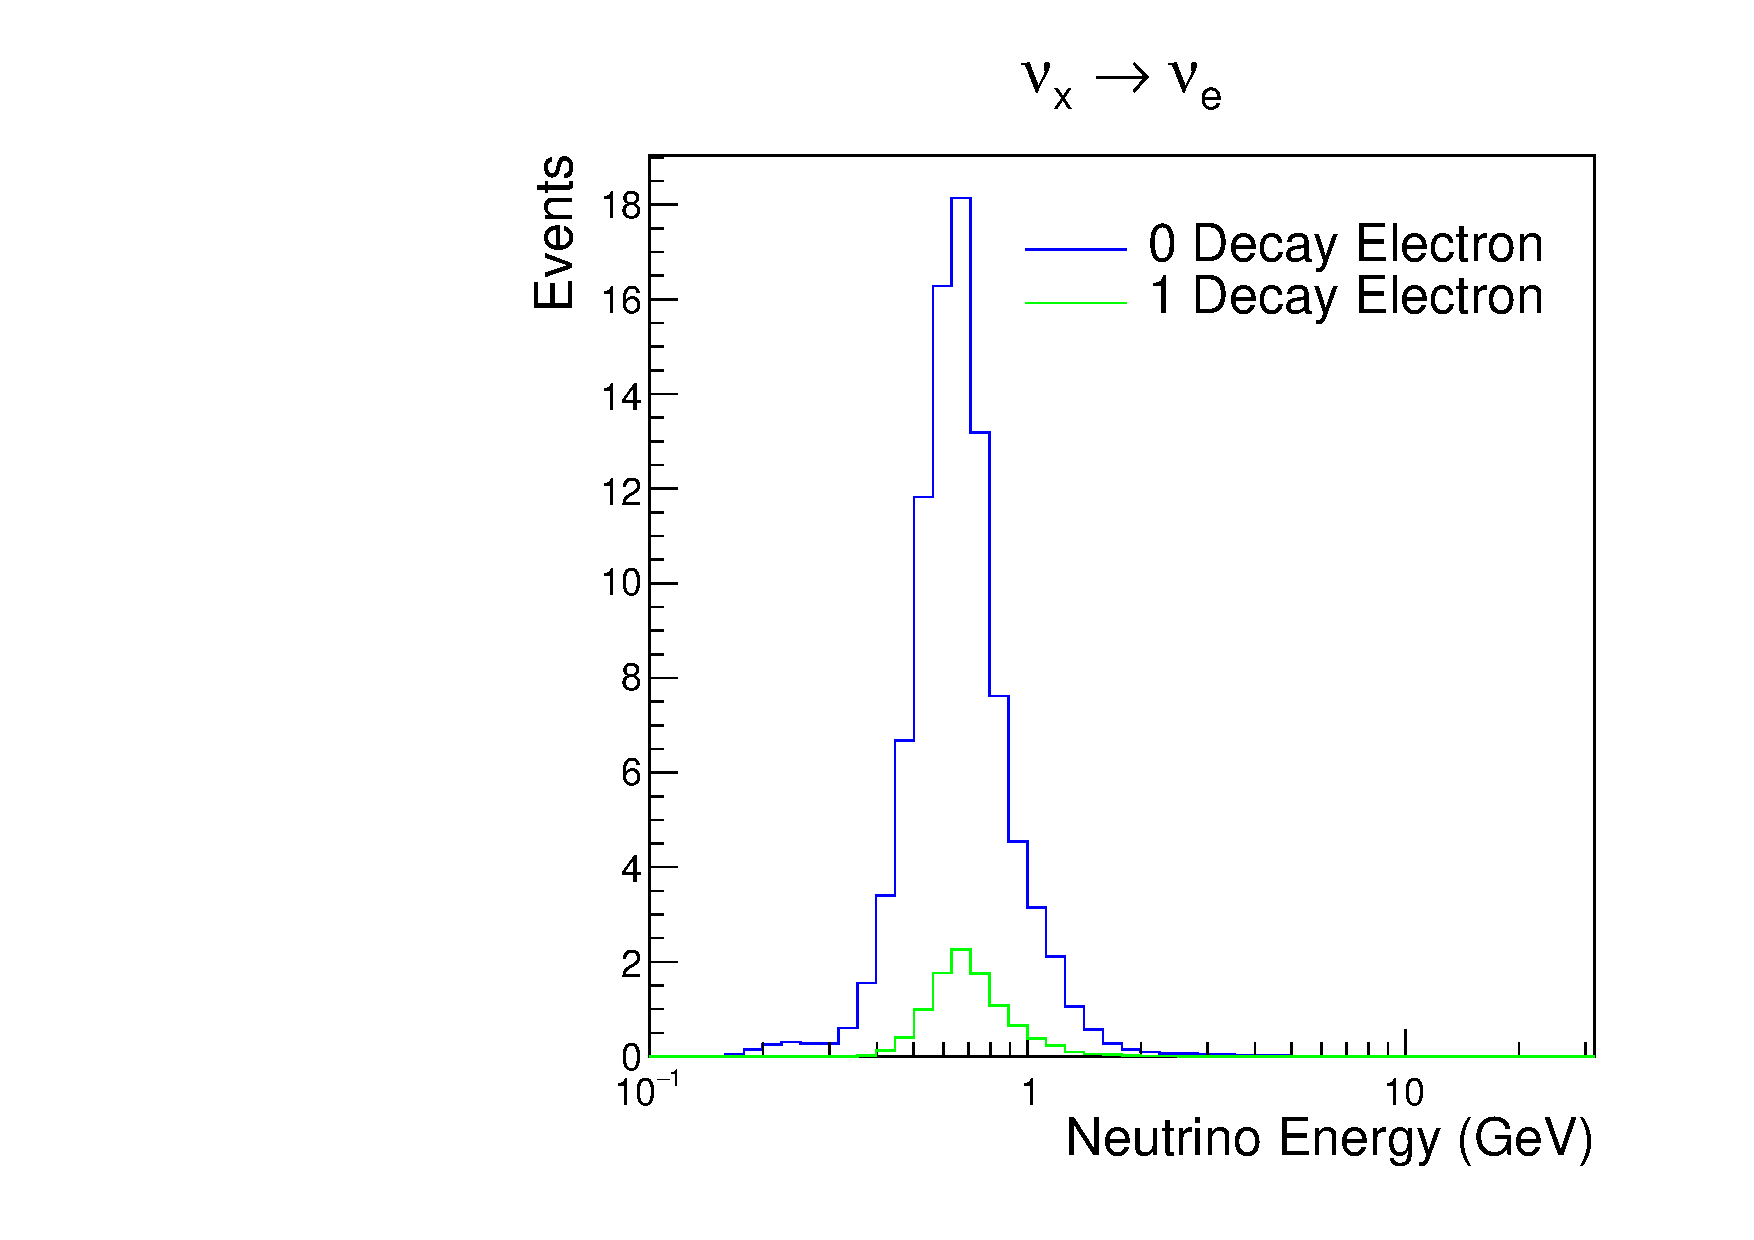
\includegraphics[width=\textwidth, trim={0mm 0mm 0mm 0mm}, clip,page=1]{Figures/Simulations/NeutrinoEnergyDist_T2K_NuE.pdf}
  \end{subfigure}%                                                                                                                                                                                         
  \begin{subfigure}[t]{0.49\textwidth}
    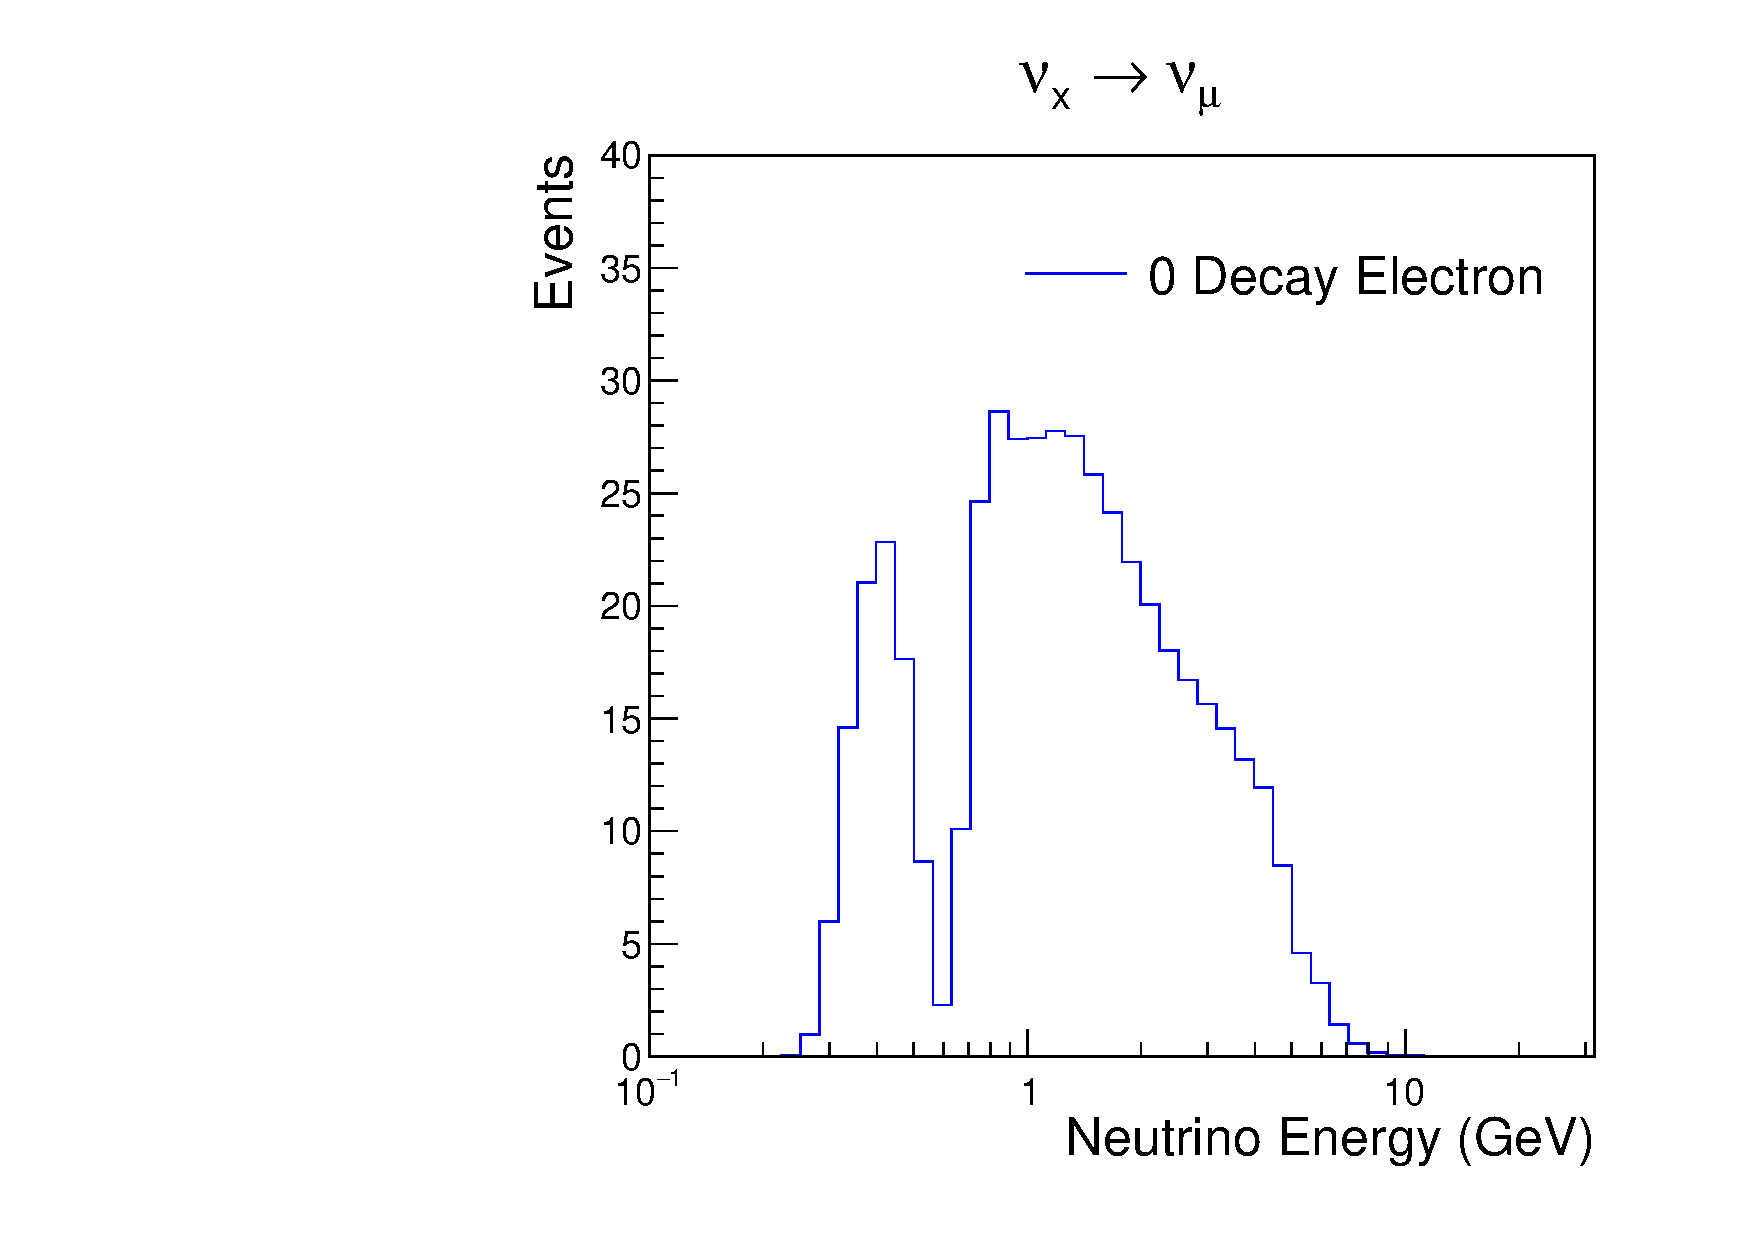
\includegraphics[width=\textwidth, trim={0mm 0mm 0mm 0mm}, clip,page=1]{Figures/Simulations/NeutrinoEnergyDist_T2K_NuMu.pdf}
  \end{subfigure}
  \caption{The predicted neutrino flux of the beam neutrinos, illustrated as a function of neutrino energy. The predictions are broken down by the number of decay electrons associated with the particular events. All systematic dials are set to their nominal values and the Asimov A oscillation parameters are assumed.}
  \label{fig:Simulations_NeutrinoEnergyDistribution_T2K}
\end{figure}

  \chapter{Sample Selections and Systematics}
\label{chap:SelsAndSysts}

\section{Systematic Uncertainties}
\label{sec:SelsAndSysts_Systs}

The systematics for this uncertainty are split into the groups, or blocks, depending on their purpose. They consist of flux uncertainties, neutrino-matter interaction systematics and detector efficiencies. There are also uncertainties on the oscillation parameters which this analysis will not be sensitive to, \delmsqsol and \sinsqsol. As described in \autoref{chap:MarkovChainMonteCarlo}, each model parameter used within this analysis requires a prior uncertainty. This is provided via separate covariance matrices for each block. The covariance matrices can include prior correlations between parameters within a single block, but the separate treatment means prior uncertainties can not be included for parameters in different groups. Alternatively, some parameters have no reasonably motivated uncertanities. These parameters are assigned flat priors which do not change the likelihood penalty. The flux, neutrino interaction and detector modelling has already been discussed in \autoref{sec:Simulations_Simulation}. The uncertainties invoked within these models are described below.

\subsection{Beam Flux}
\label{sec:SelsAndSysts_Systs_BeamFlux}

The neutrino beam flux systematics are based upon our uncertainty in the modelling of the components of the beam. This includes: the hadron production model and their re-interactions, the shape, intensity and alignment of the beam with respect to the target, and the uniformity of the magnetic field produced by the horn, alongside other effects. The uncertainty, as a function of neutrino energy, is illustrated in \autoref{fig:SelsAndSysts_BeamFluxSysts} which includes the total uncertainty as well as the individual components. The uncertainty for events below, and much higher than, the peak neutrino energy is dominated by hadron production and re-interaction systematics. The beam profile and alignment of the proton beam dominates the systematic uncertainty for events with \quickmath{E_{\nu} \sim 1\text{GeV}}. 

\begin{figure}[h]
  \begin{subfigure}[t]{\textwidth}
    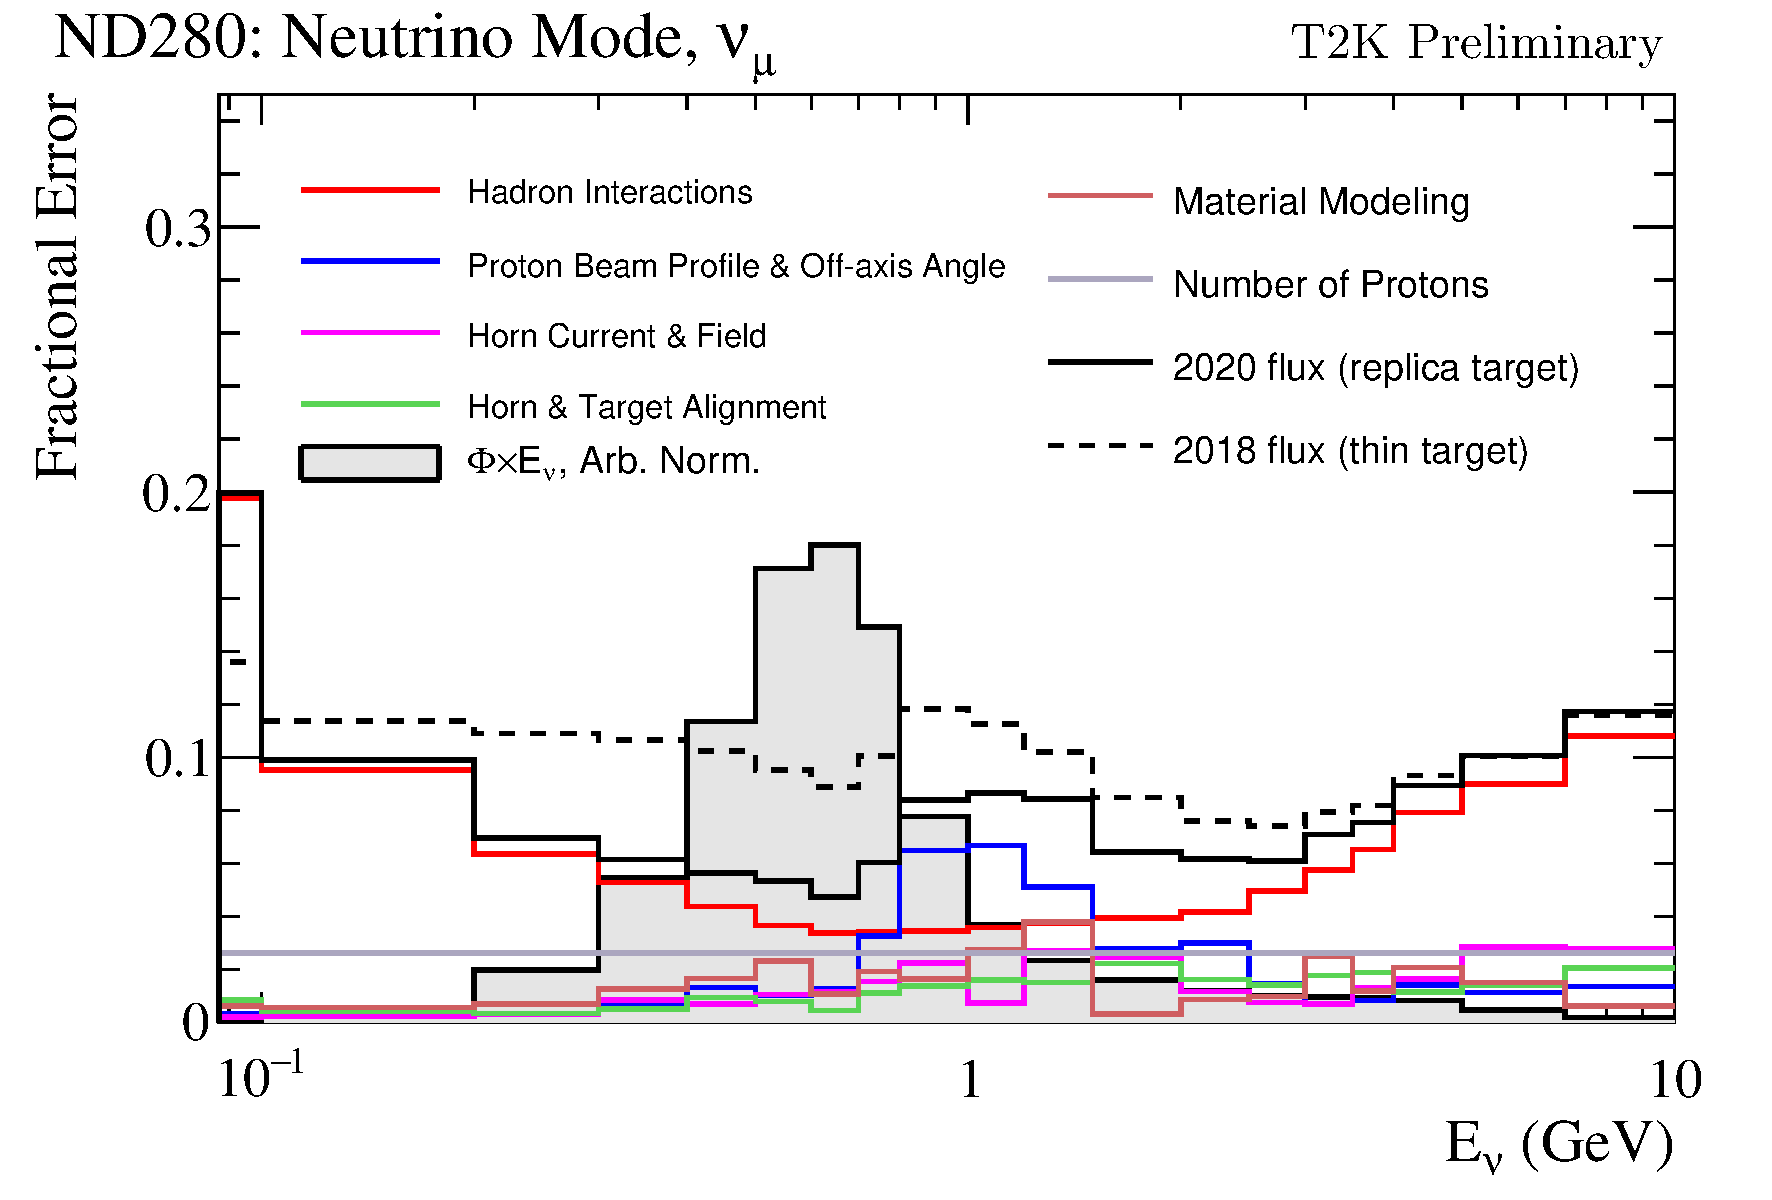
\includegraphics[width=\textwidth, trim={0mm 0mm 0mm 0mm}, clip,page=1]{Figures/Selections/flux_uncertainty_covariance_plots_addcorrnd_compwv3_flux_error_t2k_nd5_fhc_numu.pdf}
  \end{subfigure}
  %\begin{subfigure}[t]{\textwidth}
  %  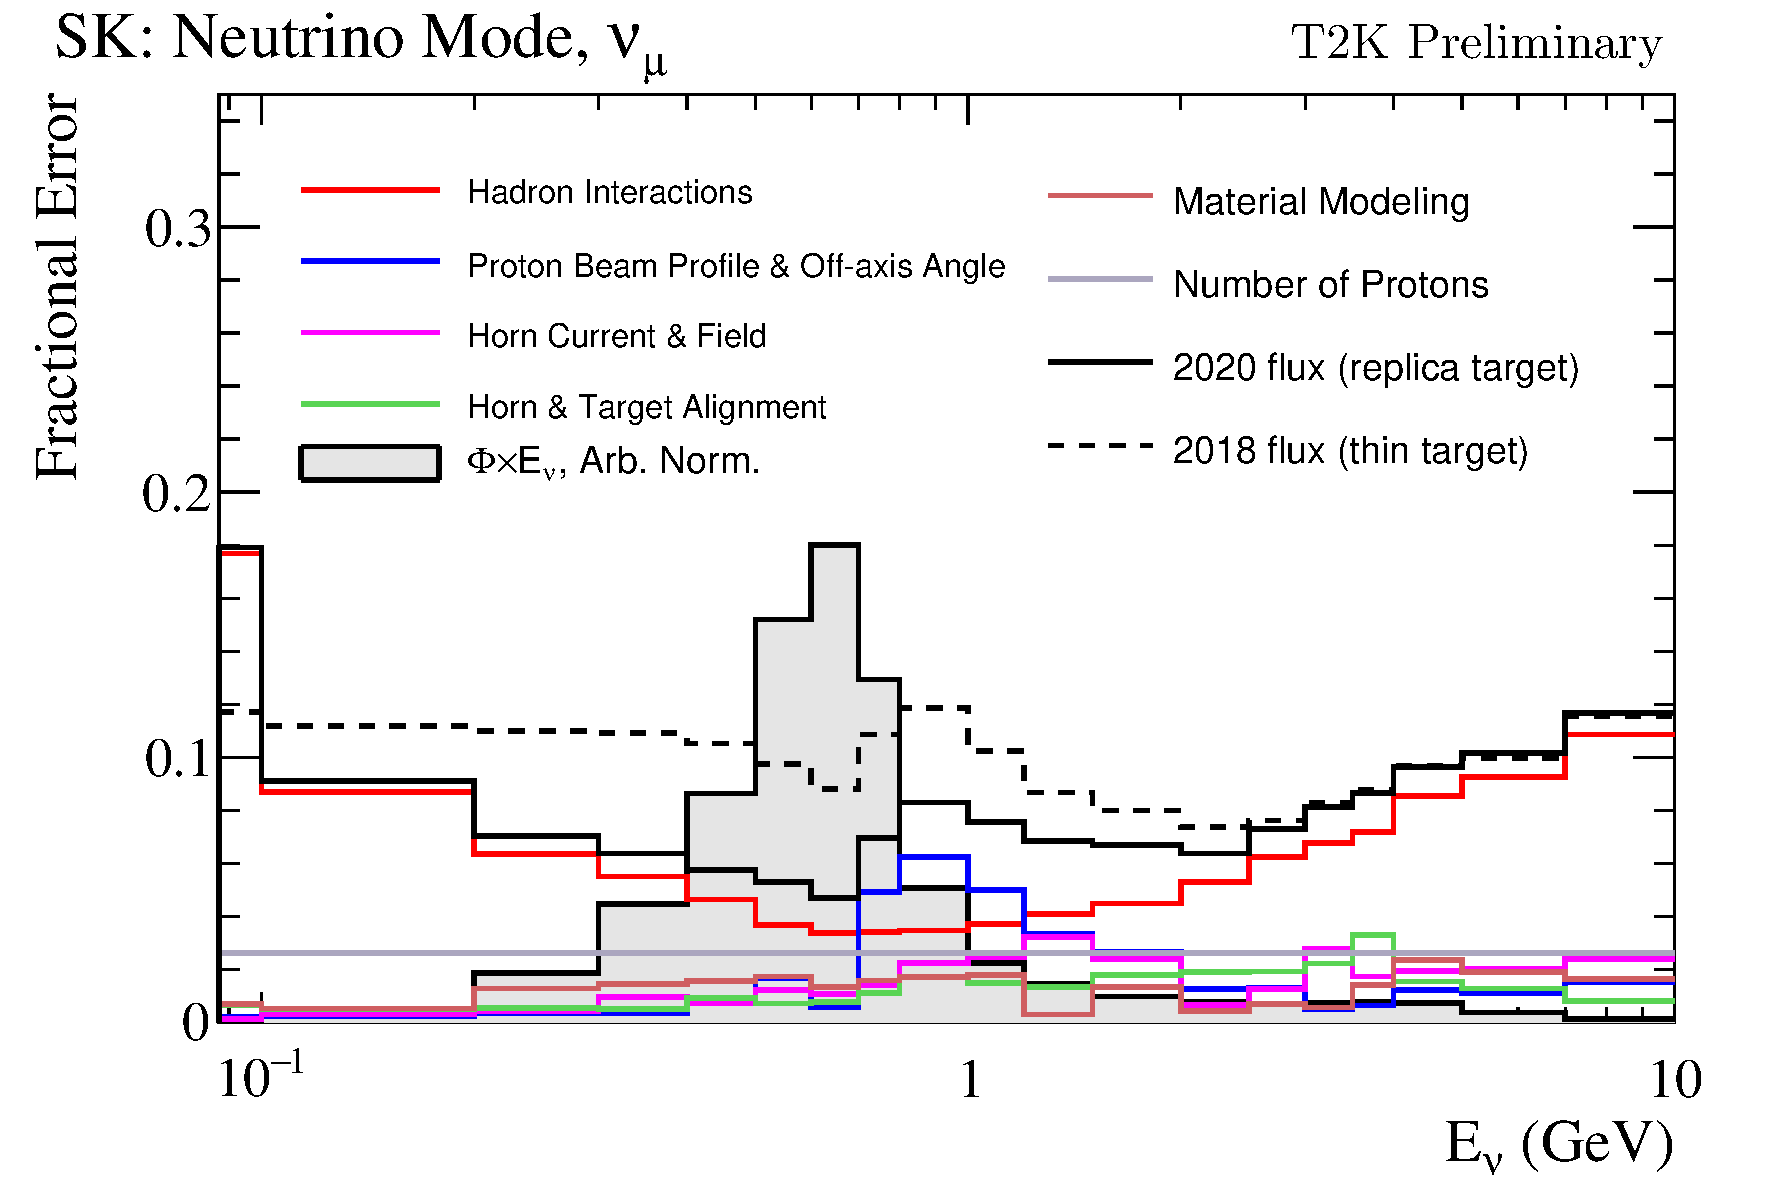
\includegraphics[width=\textwidth, trim={0mm 0mm 0mm 0mm}, clip,page=1]{Figures/Selections/flux_uncertainty_covariance_plots_addcorrnd_compwv3_flux_error_t2k_sk_fhc_numu.pdf}
  %\end{subfigure}
  \caption{The total uncertainty evaluated on the near detector \quickmath{\nu_{\mu}} flux prediction constrained by the replica-target data, illustrated as a function of neutrino energy. The solid(dashed) line indicates the uncertainty used within this analysis(the T2K 2018 analysis). The solid histogram indicates the neutrino flux as a function of energy. Figure taken from \cite{t2k_tn_354}.}
  \label{fig:SelsAndSysts_BeamFluxSysts}
\end{figure}

The beam flux uncertainties are described by one hundred parameters. They are split between both ND280 and SK detectors and binned by neutrino flavour: \quickmath{\nu_{\mu}}, \quickmath{\bar{\nu}_{\mu}}, \quickmath{\nu_{e}} and \quickmath{\bar{\nu}_{e}}. The response is then broken down as a function of neutrino energy. The bin density in the neutrino energy is the same for the FHC-\quickmath{\nu_{\mu}} and RHC-\quickmath{\bar{\nu}_{\mu}}, and narrows for neutrino energies close to the oscillation maxima of \quickmath{E_{\nu} = 0.6\text{GeV}}. This binning is specified in \autoref{tab:SelsAndSysts_BeamFluxBinEdges}. All of these systematic uncertanties are applied as normalisation parameters with Gaussian priors centered at \quickmath{1.0} and error specified from a covariance matrix provided by the T2K beam group.

\begin{table}[ht!]
    \centering
    \begin{tabular}{c|c|c}
      \hline
      Neutrino Flavour & Sign & Neutrino Energy Bin Edges (GeV) \\
      \hline
      \quickmath{\mu} & Right & \quickmath{0.,0.4,0.5,0.6,0.7,1.,1.5,2.5,3.5,5.,7.,30.} \\
      \quickmath{\mu} & Wrong & \quickmath{0.,0.7,1.,1.5,2.5,30.} \\
      \quickmath{e} & Right & \quickmath{0.,0.5,0.7,0.8,1.5,2.5,4.,30.} \\
      \quickmath{e} & Wrong & \quickmath{0.,2.5,30.} \\
      \hline
      \hline
    \end{tabular}
    \caption{The neutrino energy binning for the different neutrino flavours. ``Right'' sign indicates neutrinos in the FHC beam and antineutrinos in the RHC beam mode. ``Wrong'' sign indicates antineutrinos in the FHC beam and neutrinos in the RHC beam mode. The binning of the detector response is identical for the FHC and RHC modes as well as at ND280 and SK.}
    \label{tab:SelsAndSysts_BeamFluxBinEdges}
\end{table}

\subsection{Atmospheric Flux}
\label{sec:SelsAndSysts_Systs_AtmFlux}
The atmospheric neutrnio flux is modelled by the HKKM model, however 16 systematic uncertainties are applied to control the normalisation of each neutrino flavour, energy and direction. All of the parameters are given Gaussian priors centered at \quickmath{0} and width \quickmath{1.}. They are summarised below:

\begin{itemize}
\item \textbf{Absolute Normalisation}: The overall normalisation of each neutrino flavour is controlled by two indpendent systematic uncertainties, for \quickmath{E_{\nu} < 1\text{GeV}} and \quickmath{E_{\nu} > 1\text{GeV}}, respectively. This is driven mostly by hadronic interaction uncertainties for the production of pions and kaons \cite{Honda_2007}. The strength of the response is dependent upon the neutrino energy.
\item \textbf{Relative Normalisation}: Uncertainties on the ratio of \quickmath{(\nu_{\mu} + \bar{\nu}_{\mu})/(\nu_{e} + \bar{\nu}_{e})} are controlled by the difference between the HKKM model \cite{Honda_2007}, FLUKA \cite{etde_20239111} and Bartol models \cite{Barr_2004}. Three independent parameters are applied in the energy ranges: \quickmath{E_{\nu} < 1\text{GeV}}, \quickmath{1\text{GeV} < E_{\nu} < 10 \text{GeV}}, and \quickmath{E_{\nu} > 10\text{GeV}}.
\item \textbf{\quickmath{\nu}/\quickmath{\bar{\nu}} Normalisation}: The uncertainties in the \quickmath{\pi^{+}/\pi^{-}} (and kaon equivalent) produce uncertainties in the flux of \quickmath{\nu/\bar{\nu}}. The response is applied in the same way as the relative normalisation parameters.
\item \textbf{Up/Down and Vertical/Horizontal Ratio}: Similar to the above two systematics, the difference between the HKKM, FLUKA and Bartol model predictions, as a function of \quickmath{\cos(\theta_{Z})}, is used to control the normalisation of events as a function of zenith angle.
\item{\textbf{\quickmath{K/\pi} Ratio}}: Higher energy neutrinos (\quickmath{E_{\nu} < 10\text{GeV}}) become dependent upon kaon decay as the dominant source of neutrinos. Measurements of the ratio of \quickmath{K/\pi} \cite{Ambrosini1998-er} are used to control the systematic uncertainty of the expected ratio of pion and kaon production.
\item \textbf{Solar Activity}: As the 11-year solar cycle can affect the Earth's magnetic field, the flux of primary cosmic rays is modulated across the same period. The uncertainity is calculated by taking a \quickmath{\pm 1} year variation, equating to a \quickmath{10\%} uncertainty for the SK-IV period.
\item \textbf{Atmospheric Density}: The height of the interaction of the primary cosmic rays is dependent upon the atmospheric density. The HKKM assumes the US standard 1976 \cite{USStandardAtm} profile. This systematic controls the uncertainty in that model.
\end{itemize}

Updates to the HKKM and Bartol models are underway to use a similar tuning technique to that used in the beam flux predictions. After those updates, it may be possible to include correlations in the hadron production uncertanty systematics for beam and atmospheric flux predictions.

\subsection{Neutrino Interaction}
\label{sec:SelsAndSysts_Systs_Interaction}


  \chapter{Oscillation Probability Calculation}
\label{chap:OscillationProbability}

It is important to understand how and where the sensitivity to the oscillation parameters comes from for both atmospheric and beam samples. An overview of how these samples observe changes in \dcp, \delmsqatm, and \sinsqatm affect these samples is given in \autoref{sec:Oscillation_Overview}. This section also explains the additional complexities involved when performing an atmospheric neutrino analysis as compared to a beam-only analysis.

Without additional techniques, atmospheric sub-GeV upward-going neutrinos (\quickmath{E_{\nu} < 1.33\text{GeV}, \cos(\theta_{Z})<0.}) can artificially inflate the sensitivity to \dcp due to the quickly varying oscillation probability in this region. Therefore, a ``sub-sampling'' approach has been developed to reduce these biases ensuring accurate and reliable sensitivity measurements. This technique ensures that small-scale unresolvable features of the oscillation probability have been averaged over whilst the large-scale features in the oscillation probability are unaffected. The documentation and validation of this technique are found in \autoref{sec:Oscillation_FastOscillations}. The oscillation probability calculation is computationally intensive due to the large number of matrix multiplications needed. Consequently, the \texttt{CUDAProb3} implementation choice made within the fitting framework, as detailed in \autoref{sec:Oscillation_CalculationEngine}, ensures that the analysis can be done in a timely manner.

Whilst the beam neutrinos are assumed to propagate through a constant density slab of material, the density variations through the Earth result in more complex oscillation patterns for atmospheric neutrinos. Furthermore, the uncertainty in the electron density can modify the oscillation probability for the denser core layers of the Earth. The model of the Earth used within this analysis is detailed in \autoref{sec:Oscillation_MatterDensity}. This includes information about the official SK-only methodology as well as improvements that have been made to remove some of the approximations used in that analysis. Another complexity of atmospheric neutrinos oscillation studies is that the height of production in the atmosphere is not known on an event-by-event basis. An analytical averaging technique that approximates the uncertainty of the oscillation probability has been followed, with the author of this thesis being responsible for the implementation and validation. This implementation of an external technique is illustrated in \autoref{sec:Oscillation_ProdHAvergaing}.

\section{Overview}
\label{sec:Oscillation_Overview}

\finish{Should this be moved into an earlier chapter? The selections chapter references the matter resonance which has not yet been explained at that point}

The analysis presented within this thesis focuses on the determination of oscillation parameters from atmospheric and beam neutrinos. Whilst subject to the same oscillation formalism, the way in which the two samples have sensitivity to the different oscillation parameters differs significantly.

Atmospheric neutrinos have a varying baseline, or ``path length'', \quickmath{L}, such that the distance each neutrino travels before interacting is dependent upon the zenith angle, \quickmath{\theta_{Z}}. As primary cosmic rays can interact anywhere between the Earth's surface and \quickmath{\sim50\text{km}} above that, the height, \quickmath{h}, in the atmosphere at which the neutrino was generated also affects the path length,

\begin{equation}
  L = \sqrt{\left(R_{E} + h\right)^{2} - R_{E}^{2} \left(1 - \cos^{2} \left(\theta_{Z} \right) \right)} - R_{E}\cos(\theta_{Z}).
\end{equation}

Where \quickmath{R_{E} = 6,371\text{km}} is the Earth's radius. Consequently, the oscillation probability is dependent upon two parameters, \quickmath{\cos(\theta_{Z})} and \quickmath{E_{\nu}}.

The oscillation probability used within this analysis is based on \cite{Barger:1980tf}. The neutrino wavefunction in the vacuum Hamiltonian evolves in each layer of constant matter density via

\begin{equation}
  i \frac{d\psi_{j}(t)}{dt} = \frac{m_{j}^{2}}{2E_{\nu}} \psi_{j}(t) - \sum_{k} \sqrt{2} G_{F} N_{e} U_{ej} U_{ke}^{\dagger} \psi_{k}(t),
\end{equation}

where \quickmath{m_{j}^{2}} is the square of the \quickmath{j^{th}} vacuum eigenstate mass, \quickmath{E_{\nu}} is the neutrino energy, \quickmath{G_{F}} is Fermi's constant, \quickmath{N_{e}} is the electron number density and \quickmath{U} is the PMNS matrix. The transformation \quickmath{N_{e} \rightarrow -N_{e}} and \quickmath{\delta_{CP} \rightarrow -\delta_{CP}} is applied for antineutrino propagation. Thus, a model of the Earth's density is required for neutrino propagation. Following the official SK-only methodology \cite{thesis_roger}, this analysis uses the Preliminary Reference Earth Model (PREM) \cite{Dziewonski1981-sp} which provides piecewise cubic polynomials as a function of the Earth's radius. This density profile is illustrated in \autoref{fig:Oscillation_SK_PREMModelApproximation}. As the propagator requires layers of constant density, the SK methodology approximates the PREM model by using four layers of constant density \cite{thesis_roger}, detailed in \autoref{tab:NeutrinoOscillationPhysics_PREMModel}.

\begin{figure}[h]
  \begin{subfigure}[t]{0.8\textwidth}
    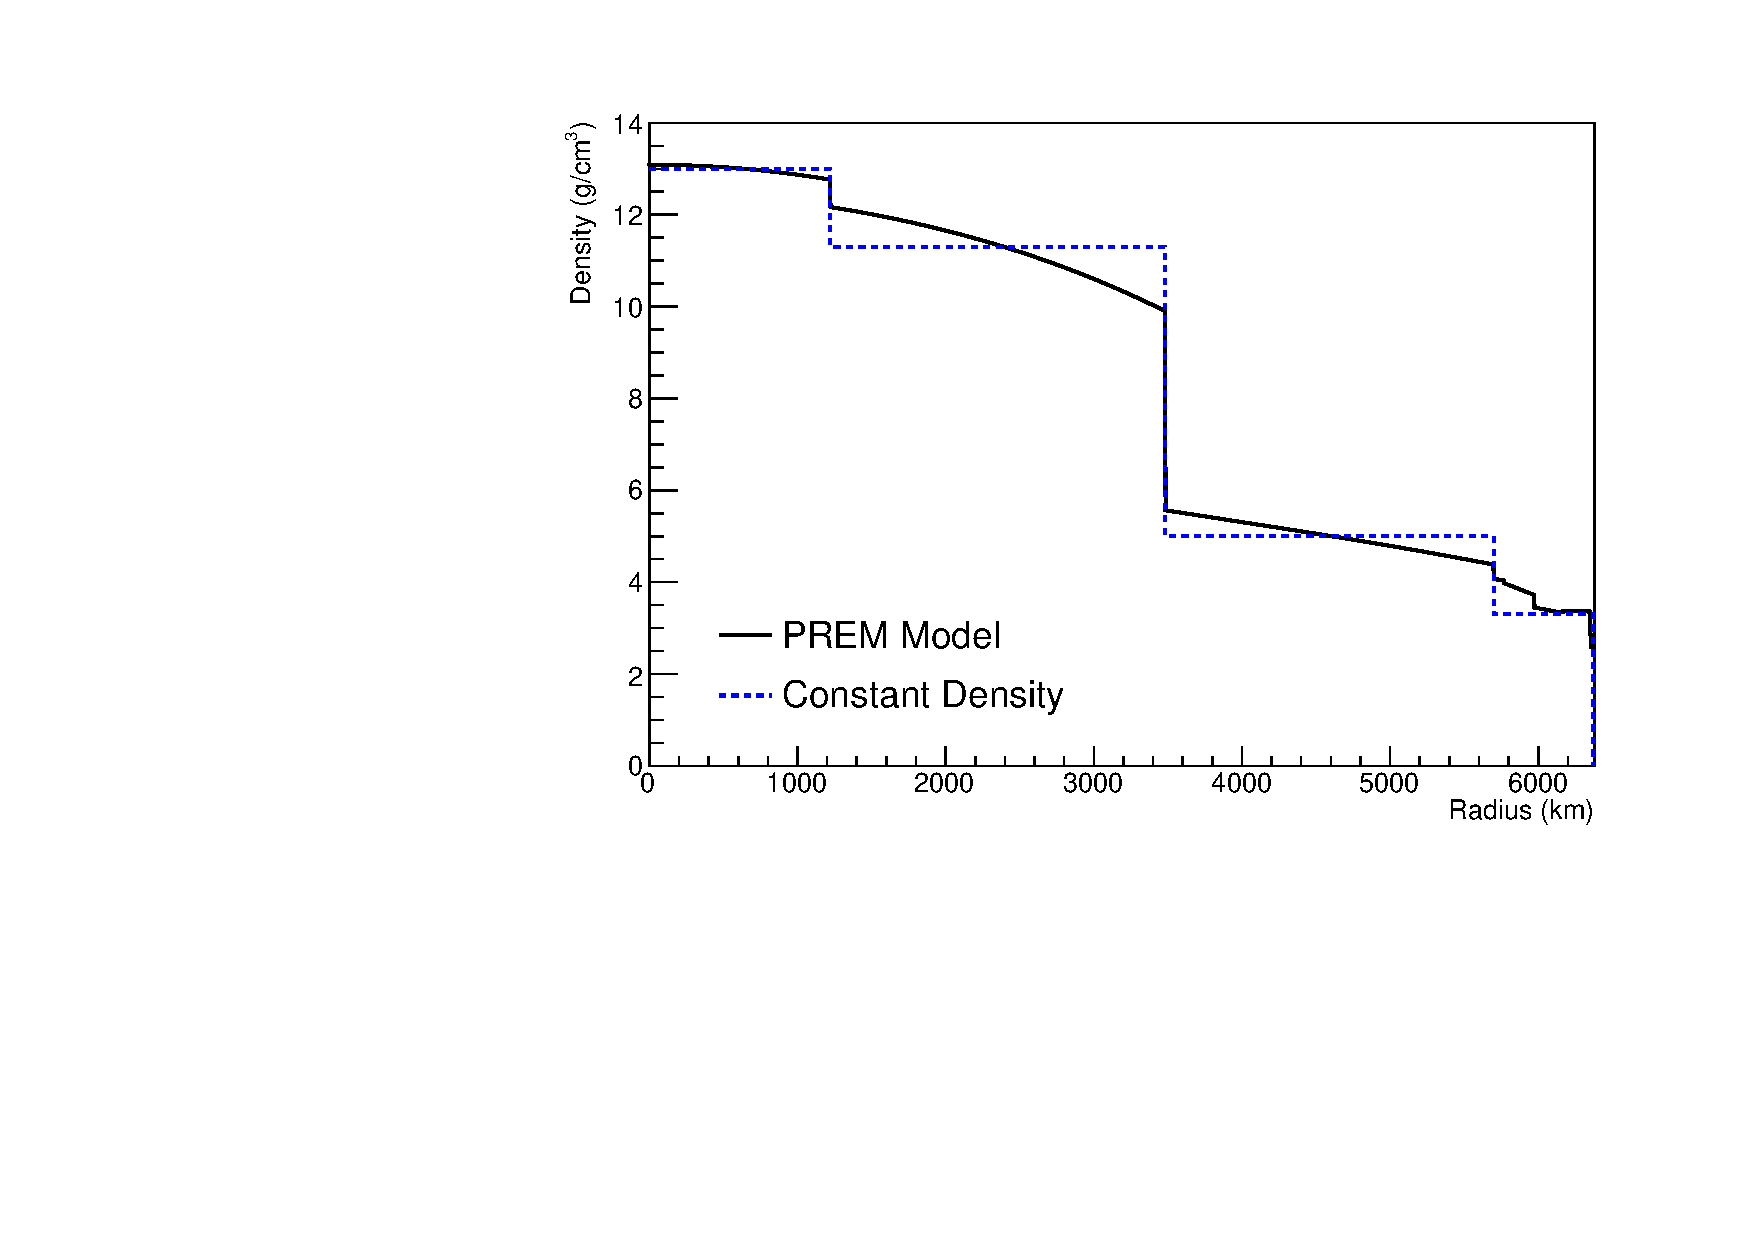
\includegraphics[width=\textwidth, trim={0mm 0mm 0mm 0mm}, clip,page=1]{Figures/Oscillation/DensityComparison.pdf}
  \end{subfigure}
  \caption{The density of the Earth given as a function of the radius, as given by the PREM model (Black), and the constant density four-layer approximation (Blue), as used in the official SK-only analysis.}
  \label{fig:Oscillation_SK_PREMModelApproximation}
\end{figure}

\begin{table}[ht!]
    \centering
    \begin{tabular}{c|c|c|c}
      \hline
      Layer & Outer Radius [\quickmath{\text{km}}] & Density [\quickmath{\text{g/cm}^{3}}] & Chemical composition (Z/A) \\
      \hline
      Inner Core & \quickmath{1220} & \quickmath{13} & \quickmath{0.468 \pm 0.029} \\
      Outer Core & \quickmath{3480} & \quickmath{11.3} & \quickmath{0.468 \pm 0.029} \\
      Lower Mantle & \quickmath{5701} & \quickmath{5.0} & \quickmath{0.496} \\
      Transition Zone & \quickmath{6371} & \quickmath{3.3} & \quickmath{0.496} \\
      \hline
    \end{tabular}
    \caption{Description of the four layers of the Earth invoked within the constant density approximation of the PREM model \cite{Dziewonski1981-sp}.}
    \label{tab:NeutrinoOscillationPhysics_PREMModel}
\end{table}

The atmospheric neutrino oscillation probabilities can be presented as two dimensional ``oscillograms'' as illustrated in \autoref{fig:Oscillation_SK_BasicOscillogram}. The distinct discontinuities, as a function of \quickmath{\cos(\theta_{Z})}, are due to the discontinous density in the PREM model.

\begin{figure}[h]
  \begin{subfigure}[t]{0.8\textwidth}
    \includegraphics[width=\textwidth, trim={0mm 0mm 0mm 0mm}, clip,page=1]{Figures/Oscillation/BasicOscillogramWithNotes.pdf}
  \end{subfigure}
  \caption{An ``oscillogram'' that depicts the \quickmath{P(\nu_\mu \rightarrow \nu_e)} oscillation probability as a function of neutrino energy and cosine of the zenith angle. The zenith angle is defined such that \quickmath{\cos(\theta_{Z}) = 1.0} represents neutrinos that travel from directly above the detector. The four-layer constant density PREM model approximation is used and Asimov A oscillation parameters are assumed (\autoref{tab:Theory_ParameterSets}).}
  \label{fig:Oscillation_SK_BasicOscillogram}
\end{figure}

Atmospheric neutrinos have sensitivity to \dcp through the overall event rate. \autoref{fig:Oscillation_SK_DCPSensitivity} illustrates the difference in oscillation probability between CP-conserving (\quickmath{\delta_{CP} = 0.}) and a CP-violating (\quickmath{\delta_{CP} = -1.601}) value taken from Asimov A oscillation parameter set (\autoref{tab:Theory_ParameterSets}). The result is a complicated oscillation pattern in the appearance probability for sub-GeV upgoing neutrinos. The detector does not have sufficient resolution to resolve these individual patterns so the sensitivity to \dcp for atmospheric neutrinos comes via the overall normalisation of these events.

The presence of matter means that the effect \dcp has on the oscillation probability is not equal between neutrinos and antineutrinos. Furthermore, the interaction cross-section for neutrinos is larger than antineutrinos so the two effects have to be disentangled. These effects are further convoluted by detector efficiencies as SK cannot distinguish neutrinos and antineutrinos well. Furthermore, the sample selections discussed in \autoref{sec:SelsAndSysts_Sels_Atms} have difference efficiencies for neutrino-antineutrino selections. All of these effects lead to a difference in the number of neutrinos detected compared to antineutrinos. This changes how the \dcp normalisation term is observed, resulting in a very complex sensitivity to \dcp.

\begin{figure}[h]
  \begin{subfigure}[t]{\textwidth}
    \includegraphics[width=\textwidth, trim={0mm 0mm 0mm 0mm}, clip,page=1]{Figures/Oscillation/AtmDCPSens.pdf}
  \end{subfigure}
  \caption{The effect of \dcp for atmospheric neutrinos given in terms of the neutrino energy and zenith angle. This oscillogram compares the \quickmath{P(\nu_{\mu} \rightarrow \nu_{e})} oscillation probability for a CP conserving (\quickmath{\delta_{CP}=0.0}) and a CP violating (\quickmath{\delta_{CP}=-1.601}) value taken from the Asimov A parameter set. The other oscillation parameters assume the Asimov A oscillation parameter set given in \autoref{tab:Theory_ParameterSets}.}
  \label{fig:Oscillation_SK_DCPSensitivity}
\end{figure}

The vacuum and matter oscillation probabilities for \quickmath{P(\nu_{e} \rightarrow \nu_{e})} and \quickmath{P(\bar{\nu}_{e} \rightarrow \bar{\nu}_{e})} are presented in \autoref{fig:Oscillation_SK_VacuumMatter}, where the PREM model has been assumed. The oscillation probability for both neutrinos and antineutrinos is affected in the presence of matter. However, the resonance effects around \quickmath{O(5)\text{GeV}} only occur for neutrinos in normal mass hierarchy and antineutrinos in inverse mass hierarchy. The exact position and amplitude of the resonance depend on \sinsqatm , further increasing the atmospheric neutrinos' sensitivity to the parameter.

\begin{figure}[h]
  \begin{subfigure}[t]{\textwidth}
    \includegraphics[width=\textwidth, trim={0mm 0mm 0mm 0mm}, clip,page=1]{Figures/Oscillation/MatterEffect.pdf}
  \end{subfigure}
  \caption{An illustration of the matter-induced effects on the oscillation probability, given as a function of neutrino energy and zenith angle. The top row of panels gives the \quickmath{P(\nu_{e} \rightarrow \nu_{e})} oscillation probability and the bottom row illustrates the \quickmath{P(\bar{\nu}_{e} \rightarrow \bar{\nu}_{e})} oscillation probability. The left column highlights the oscillation probability in a vacuum, whereas the middle and right column represents the oscillation probabilities when the four-layer fixed density PREM model is assumed. All oscillation probabilities assume the ``Asimov A'' set given in \autoref{tab:Theory_ParameterSets}, but importantly, the right column sets an inverted mass hierarchy. The ``matter resonance'' effects at \quickmath{E_{\nu} \sim 5\text{GeV}} can be seen in the \quickmath{P(\nu_{e} \rightarrow \nu_{e})} for normal mass hierarchy and \quickmath{P(\bar{\nu}_{e} \rightarrow \bar{\nu}_{e})} for inverted hierarchy.}
  \label{fig:Oscillation_SK_VacuumMatter}
\end{figure}

As the T2K beam flux is centered at the first oscillation maximum (\quickmath{E_{\nu} = 0.6\text{GeV}}), the sensitivity to \dcp is predominantly observed as a change in the event-rate of e-like samples in \quickmath{\nu/\bar{\nu}} modes. \autoref{fig:Oscillation_T2K_OscillationProbSensitivity} illustrates the \quickmath{P(\nu_\mu \rightarrow \nu_e)} oscillation probability for a range of \dcp values. %The magnitude of the oscillation peak has an approximate factor of two difference between the CP-violating values \quickmath{\delta_{CP} = \pm\pi/2} and the difference in oscillation probability between the CP-conserving
A circular modulation of the first oscillation peak (in both magnitude and position) is observed when varying throughout the allowable values of \dcp. The CP-conserving values of \quickmath{\delta_{CP}=0,\pi} have a lower(higher) oscillation maximum than the CP-violating values of \quickmath{\delta_{CP}=-\pi/2}(\quickmath{\delta_{CP}=\pi/2}). A sub-dominant shift in the energy of the oscillation peak is also present, which aids in separating the two CP-conserving values of \dcp.

\begin{figure}[h]
  \begin{subfigure}[t]{0.5\textwidth}
    \includegraphics[width=\textwidth, trim={0mm 0mm 0mm 0mm}, clip,page=1]{Figures/Oscillation/T2K_NuMu_x_NuMu_DelMsq32Sens.pdf}
    \subcaption{\delmsqatm}
  \end{subfigure}%
  \begin{subfigure}[t]{0.5\textwidth}
    \includegraphics[width=\textwidth, trim={0mm 0mm 0mm 0mm}, clip,page=1]{Figures/Oscillation/T2K_NuMu_x_NuMu_Sinsqth23Sens.pdf}
    \subcaption{\sinsqatm}
  \end{subfigure}
  \begin{subfigure}[t]{0.5\textwidth}
    \includegraphics[width=\textwidth, trim={0mm 0mm 0mm 0mm}, clip,page=1]{Figures/Oscillation/T2K_NuMu_x_NuE_DCPSens.pdf}
    \subcaption{\dcp}
  \end{subfigure}
  \caption{The oscillation probability for beam neutrino events given as a function of neutrino energy. All oscillation parameters assume the ``Asimov A'' set given in \autoref{tab:Theory_ParameterSets} unless otherwise stated. Each panel represents a change in one of the oscillation parameters whilst keeping the remaining parameters fixed.}
  \label{fig:Oscillation_T2K_OscillationProbSensitivity}
\end{figure}

T2K's sensitivity to \sinsqatm and \delmsqatm is observed as a shape-based variation of the muon-like samples, as illustrated in \autoref{fig:Oscillation_T2K_OscillationProbSensitivity}. The value of \quickmath{\Delta m^{2}_{32}} laterally shifts the position of the oscillation dip (around \quickmath{E_\nu \sim 0.6\text{GeV}}) in the \quickmath{P(\nu_\mu \rightarrow \nu_\mu)} oscillation probability. A variation of \sinsqatm is predominantly observed as a vertical shift of the oscillation dip with second-order horizontal shifts being due to matter effects. The beam neutrinos have limited sensitivity to matter effects due to the relatively shorter baseline as well as the Earth's mantle being a relatively low-density material (as compared to the Earth's core). For some values of \dcp, the degeneracy in the number of e-like events allows the mass hierarchy to be broken. This leads to a \dcp-dependent mass hierarchy sensitivity which can be seen in \autoref{fig:Oscillation_SK_BiProbabilityPlot}.

\begin{figure}[h]
  \begin{subfigure}[t]{0.65\textwidth}
    \includegraphics[width=\textwidth, trim={0mm 0mm 0mm 0mm}, clip,page=1]{Figures/Oscillation/BiProbabilityPlot.pdf}
  \end{subfigure}
  \caption{The number of electron-like events in the FHC and RHC operating mode of the beam, as a function of the oscillation probabilities. Both normal hierarchy (Solid)) and inverse hierarchy (Dashed) values of \delmsqatm are given.}
  \label{fig:Oscillation_SK_BiProbabilityPlot}
\end{figure}

Whilst all oscillation channels should be included for completeness, the computational resources required to run a fit are limited and any reasonable approximations which reduce the number of oscillation probability calculations that need to be made should be applied. The \quickmath{\nu_{e} \rightarrow \nu_{e,\mu,\tau}} (and antineutrino equivalent) oscillations can be ignored for beam neutrinos as the \quickmath{\nu_{e}/\bar{\nu}_{e}} fluxes are approximately two orders of magnitude smaller than the corresponding \quickmath{\nu_{\mu}/\bar{\nu}_{\mu}} flux. Furthermore, as the peak neutrino energy of the beam is well below the threshold for charged current tau production (\quickmath{E_\nu = 3.5\text{GeV}} \cite{Li_2018}, only a small proportion of the neutrinos produced in the beam have the required energy. For the few neutrinos that have sufficient energy, the oscillation probability is very small due to the short baseline. Whilst these approximations have be made for the beam neutrinos, the atmospheric flux of \quickmath{\nu_{e}} is of the same order of magnitude as the \quickmath{\nu_{\mu}} flux and the energy distribution of atmospheric neutrinos extends well above the tau production threshold.

\clearpage

\section{Treatment of Fast Oscillations}
\label{sec:Oscillation_FastOscillations}

As shown in \autoref{fig:Oscillation_SK_FastOscillogram}, atmospheric neutrino oscillations have a significantly more complex structure for upgoing neutrinos with energy below \quickmath{1\text{GeV}}. This is because the \quickmath{L/E} dependence of the oscillation probability in this region induces rapid variations for small changes in \quickmath{L} or \quickmath{E}. As discussed in \autoref{sec:Oscillation_Overview}, this is also the region in which atmospheric neutrinos have sensitivity to \dcp. In practice, the direction of the neutrino is inferred from the direction of the final state particles traveling in the detector, which can be poor for low-energy neutrino interactions. This creates a distinct difference from the beam neutrinos where the position of the source is very precisely known.

As a consequence of the unresolvable structure, an event rate consistent with the averaged oscillation probability is observed in the subGeV upgoing region. This creates a computational problem: A significantly large amount of Monte Carlo statistics would be required to accurately predict the number of events if Monte Carlo averaging was the only technique used. This section describes the `sub-sampling' approach developed for this analysis and compares it to the methodology used within the SK-only analysis.

\begin{figure}[h]
  \begin{subfigure}[t]{0.8\textwidth}
    \includegraphics[width=\textwidth, trim={0mm 0mm 0mm 0mm}, clip,page=1]{Figures/Oscillation/FastOscillationExample.pdf}
  \end{subfigure}
  \caption{The oscillation probability \quickmath{P(\nu_{\mu} \rightarrow \nu_{e})}, given as a function of neutrino energy and zenith angle, which highlights an example of the ``fast'' oscillations in the sub-GeV upgoing region.}
  \label{fig:Oscillation_SK_FastOscillogram}
\end{figure}

The official SK-only analysis uses the osc3++ oscillation parameter fitter \cite{thesis_roger}. To perform the fast oscillation averaging, it uses a 'nearest-neighbour' technique. For a given Monte Carlo neutrino event, the nearest twenty Monte Carlo neighbours in reconstructed lepton momentum and zenith angle are found and a distribution of their neutrino energies is built. The RMS, \quickmath{\sigma}, of this distribution is then used to compute an average oscillation probability for the given neutrino Monte Carlo event. 

For the \quickmath{i^{th}} event, the oscillation weight is calculated as

\begin{equation}
  W_{i} = \frac{1}{5} P(E_{i},\bar{L}_{i}) + \frac{1}{5} \sum_{\beta = -1, -0.5, 0.5, 1} P(E_{i} + \beta\sigma_{i},L_{\beta}),
\end{equation}

where \quickmath{P(E,L)} is the oscillation probability calculation for neutrino energy \quickmath{E} and path length \quickmath{L} and the two path lengths, \quickmath{\bar{L}_{i}} and \quickmath{L_{\beta}} are discussed below. All of the oscillation probability calculations are performed with a fixed zenith angle such that the same density profile is used.

The uncertainty in the production height is controlled by using an ``average'' production height, \quickmath{\bar{L}_{i}}, which represents the average path length computed using twenty production heights taken from the Honda flux model's prediction \cite{Honda:2011}. For a given event, the production heights are sampled in steps of \quickmath{5\%} of their cumulative distribution function. \quickmath{L_{\beta}} values are similarly calculated but instead use different combinations of four production heights,

\begin{equation}
  \begin{split}
    L_{-1.0} &= \frac{1}{4} L(45,50,55,60), \\
    L_{-0.5} &= \frac{1}{4} L(35,40,65,70), \\
    L_{+0.5} &= \frac{1}{4} L(25,30,75,68), \\
    L_{+1.0} &= \frac{1}{4} L(15,20,85,89). \\
  \end{split}
\end{equation}

This averaging technique works because of the inference between the zenith angle and the reconstructed direction of final state particles in the detector. For low-energy neutrinos, where the resolution of the true neutrino direction is poor, \quickmath{\sigma_{i}} will be large, resulting in significant averaging effects. Contrary to this, the inferred direction of high-energy neutrinos will be much closer to the true value, meaning that \quickmath{\sigma_{i}} will be smaller, culminating in small averaging effects.

In practice, these calculations are performed prior to the fit as only oscillation parameters at fixed points are considered. The MCMC technique used in this thesis requires oscillation probabilities to be evaluated at arbitary parameter values, not known \textit{a priori}. Calculating the five oscillation probabilities per event required by the SK technique is conputationally infeasible, so a differencct averaging technique is used. However, the concept of the averaging technique can be taken from it.

%In practice, this technique is performed before the fit in order to deal with the computational cost. This is possible as the Osc3++ framework uses binned oscillation parameters rather than continuous so the oscillation parameters used in the fit are known prior to run-time. The framework used in this analysis uses continuous oscillation parameters, and due to the MCMC fitting technique, there is no way to know which oscillation parameter values will be selected \textit{a priori}. Therefore, the oscillation parameter calculation has to be performed at run-time. Computing five oscillation probabilities per event would require far too many computational resources to be viable. Therefore SK technique can not be used within this analysis. 

%To perform a similar averaging as the SK analysis, a sub-sampling approach using binned oscillograms has been devised. The technique can be explained by considering a ``fine'' and ``coarse'' oscillogram. The fine oscillograms are used to define the array of \quickmath{\cos(\theta_{Z})} and \quickmath{E_{\nu}} used in the oscillation engine. The coarse oscillograms cover the same phase-space but have fewer bins, where the value of a particular coarse bin is taken as the linear average (flat prior in \quickmath{E_{\nu}} and \quickmath{\cos(\theta_{Z})}) of all fine bins which falls into it. The coarse oscillogram is then used for determining the oscillation weight for a given event. The binning which is used to calculate the oscillation probabilities, known as the `fine' binning, has \quickmath{N \times N} subdivisions per coarse bin. \autoref{fig:Oscillation_SK_SubSamplingExample} illustrates the \quickmath{N = 2} example where the assigned value to a coarse bin is the average of the four fine bins which fall in that coarse bin. Whilst the coarse bin edges do not have to be linear on either axis, the sub-division of the fine bins is linear over the range of a coarse bin.

To perform a similar averaging as the SK analysis, a sub-sampling approach using binned oscillograms has been devised. A coarsly binned oscillogram is defined in \quickmath{\cos(\theta_{Z})} and \quickmath{E_{\nu}}. For a given set of oscillation parameters, a single oscillation probability will be assigned to each coarse bin. This value will then apply to all Monte Carlo events which fall into that bin. To assign these oscillation probabilities, the probability is calculated at \quickmath{N \times N} points on a grid within a particular bin. This ensemble of oscillation probabilities is averaged to define the coarse bin's oscillation probability, assuming a flat prior in \quickmath{E_{\nu}} and \quickmath{\cos(\theta_{Z})}. \autoref{fig:Oscillation_SK_SubSamplingExample} illustrates the \quickmath{N = 2} example where the assigned value to a coarse bin is the average of the four fine bins which fall in that coarse bin. Whilst the coarse bin edges do not have to be linear on either axis, the sub-division of the fine bins is linear over the range of a coarse bin.

\begin{figure}[h]
  \begin{subfigure}[t]{\textwidth}
    \includegraphics[width=\textwidth, trim={0mm 0mm 0mm 0mm}, clip,page=1]{Figures/Oscillation/SubSamplingExample.pdf}
  \end{subfigure}
  \caption{Illustration of the averaging procedure for \quickmath{N=2}. The oscillation probabilities calculated on the finer left binning are averaged to obtain the oscillation probabilities in the coarser right binning. These averaged oscillation probabilities with the coarser binning are then applied to each event during the fit.}
  \label{fig:Oscillation_SK_SubSamplingExample}
\end{figure}

The coarse binning is defined with \quickmath{67 \times 52} bins in true neutrino energy \quickmath{\times} cosine zenith. It is picked to be identical to that provided in \cite{t2k_tn_425}. In general, the binning is logarithmically spaced in neutrino energy but has some hand-picked bin edges around the matter resonance to smoothly increased the bin density. This is to avoid smearing this region which can be well sampled by the Monte Carlo. The cosine zenith binning is approximately linearly spaced across the allowable range but the values of layer transitions are hit precisely: \quickmath{-0.8376} (core-mantle) and \quickmath{-0.4464} (mantle/transition zone). Bins are spread further apart for downgoing events as this is a region unaffected by the fast oscillation wavelengths and reduces the total number of calculations required to perform the calculation.

The choice of \quickmath{N} is justified based on two studies. Firstly, the variation of event rates of each sample is studied as a function of \quickmath{N}. For a given set of oscillation parameters thrown from the PDG prior constraints (detailed in \autoref{tab:Theory_PDGConstraints}), the oscillation probabilities are calculated using a given value of \quickmath{N}. Each sample is re-weighted and the event rate is stored. The value of \quickmath{N} is scanned from \quickmath{1}, which corresponds to no averaging, to \quickmath{19}, which corresponds to the largest computationally viable subdivision binning. The event rate of each sample at large \quickmath{N} is expected to converge to a stationary value due to the fine binning fully sampling the small-scale structure. \autoref{fig:Oscillation_SK_EventRateVariable} illustrates this behaviour for the \texttt{SubGeV\_elike\_0dcy} sample for \quickmath{9} different throws of the oscillation parameters.

\begin{figure}[h]
  \begin{subfigure}[t]{\textwidth}
    \includegraphics[width=\textwidth, trim={0mm 0mm 0mm 0mm}, clip,page=1]{Figures/Oscillation/EventRate_VariableGraphs.pdf}
  \end{subfigure}
  \caption{Event rate of the \texttt{SubGeV\_elike\_0dcy} sample as a function of the number of sub-divisions per coarse bin. Each subplot represents the event rate of the sample at a different oscillation parameter set thrown from the PDG priors detailed in \autoref{tab:Theory_PDGConstraints}. The red line in each subplot represents the mean of the event rate over the different values of sub-divisions for that particular oscillation parameter throw.}
  \label{fig:Oscillation_SK_EventRateVariable}
\end{figure}

Denoting the event rate for one sample for a given throw \quickmath{t} at each \quickmath{N} by \quickmath{\lambda_t^{N}}, the average over all considered \quickmath{N} values (\quickmath{\overline \lambda_t = \frac{1}{24} \sum_{N=1}^{24} \lambda_t^{N}}) is computed. The variance in the event rate at each \quickmath{N} is then calculated as

\begin{equation}
  \mathrm{Var}\Big[\lambda^{N}\Big] = \tfrac{1}{N_\mathrm{throws}} \sum_{t=1}^{N_\mathrm{throws}} \left(\lambda_t^{N} - \overline \lambda_t\right)^2 - \left[\tfrac{1}{N_\mathrm{throws}} \sum_{t=1}^{N_\mathrm{throws}} \left(\lambda_t^{N} - \overline \lambda_t\right)\right]^2 .
  \label{eq:Oscillation_SK_Variance}
\end{equation}

In practice the following procedure is undertaken. For a particular throw, the difference between the event rate at a particular choice of \quickmath{N} and the mean of the distribution is calculated. This is illustrated in \autoref{fig:Oscillation_SK_ExampleCalculation}. This value is then calculated for all the \quickmath{2000} throws, generaring a distribution of \quickmath{\lambda_t^{N} - \overline \lambda_t}. This is repeated for each of the values of \quickmath{N} considered within this study. The distributions of this value, for \quickmath{N = \{1,5\}}, are given in \autoref{fig:Oscillation_SK_DifferenceDistribution}. As expected, the distribution gets narrower and tends towards zero for the higher values of \quickmath{N}. 

\begin{figure}[h]                                                                                                                                                                                          
  \begin{subfigure}[t]{\textwidth}
    \includegraphics[width=\textwidth, trim={0mm 0mm 0mm 0mm}, clip,page=1]{Figures/Oscillation/ExampleCalculation.pdf}
  \end{subfigure}
  \caption{Event rate of the \texttt{SubGeV\_elike\_0dcy} sample, for a particular oscillation parameter throw, as a function of the number of sub-divisions, \quickmath{N}, per coarse bin. The difference between the mean event rate (red), \quickmath{\bar{\lambda}}, and the event rate at \quickmath{N=1}, \quickmath{\lambda^{N=1}} is defined as \quickmath{\lambda^{N} - \bar{\lambda}} and illustrated by the blue arrow.}
  \label{fig:Oscillation_SK_ExampleCalculation}
\end{figure}

\begin{figure}[h]                                                                                                                                                                                          
  \begin{subfigure}[t]{\textwidth}
    \includegraphics[width=\textwidth, trim={0mm 0mm 0mm 0mm}, clip,page=1]{Figures/Oscillation/DifferenceInEventRateToMean.pdf}
  \end{subfigure}
  \caption{The distribution of \quickmath{\lambda^{N} - \bar{\lambda}} for various values of \quickmath{N}. As expected, the distribution gets narrower for larger values of \quickmath{N}.}
  \label{fig:Oscillation_SK_DifferenceDistribution}
\end{figure}

The aim of the study is to find the lowest value of \quickmath{N} such that this variance is below \quickmath{0.001}. This utilises the width of the distributions given in \autoref{fig:Oscillation_SK_DifferenceDistribution}. This is the typical threshold used by T2K fitters to validate systematic implementation so has been set as the same criteria. The results of this study for each atmospheric sample used within this thesis are illustrated in \autoref{fig:Oscillation_SK_EventRateVariance} for \quickmath{2000} throws of the oscillation parameters. As can be seen, the variance is below the threshold at \quickmath{N = 10}, and is driven primarily by the \texttt{SubGeV\_mulike\_1dcy} and \texttt{SubGeV\_elike\_0dcy} samples.

%\begin{figure}[h]
\begin{sidewaysfigure}
  \begin{subfigure}[t]{\textwidth}
    \includegraphics[width=\textwidth, trim={0mm 0mm 0mm 0mm}, clip,page=1]{Figures/Oscillation/EventRate_VarianceGraphs.pdf}
  \end{subfigure}
  \caption{Variance of event rate for each atmospheric sample as a function of the number of sub-divisions per coarse bin. The solid red line indicates the \quickmath{0.1\%} threshold and the dashed red line indicates the variance at a sub-division \quickmath{N = 10}.}
  \label{fig:Oscillation_SK_EventRateVariance}
\end{sidewaysfigure}
  %\end{figure}
  

The second study to determine the value of \quickmath{N} is as follows. The likelihood for each sample is computed against an Asimov data set created with Asimov A oscillation parameters (\autoref{tab:Theory_ParameterSets}). Following \autoref{eq:Oscillation_SK_Variance}, the variance of the log-likelihood over all considered \quickmath{N} is computed. The results are shown in \autoref{fig:Oscillation_SK_LLHVariance}. 

%\begin{figure}[h]
\begin{sidewaysfigure}
  \begin{subfigure}[t]{\textwidth}
    \includegraphics[width=\textwidth, trim={0mm 0mm 0mm 0mm}, clip,page=1]{Figures/Oscillation/Likelihood_VarianceGraphs.pdf}
  \end{subfigure}
  \caption{Variance of sample likelihood, when compared to `Asimov data' set at Asimov A, for each atmospheric sample as a function of the number of sub-divisions per coarse bin. The solid red line indicates the \quickmath{0.1\%} threshold and the dashed red line is a graphical indication of the variance at a sub-division \quickmath{N = 10}.}
  \label{fig:Oscillation_SK_LLHVariance}
\end{sidewaysfigure}
%\end{figure}

A choice of \quickmath{N=10} sub-divisions per coarse bin has a variance in both event rate and log-likelihood residuals less than the required threshold of \quickmath{0.001}. The largest value of the likelihood variance is of order \quickmath{10^{-7}}, corresponding to an error on the log-likelihood of about \quickmath{3\times 10^{-4}} which is small enough to be negligible for the oscillation analysis.

\autoref{fig:Oscillation_SK_SmearingImplementation} illustrates the effect of the smearing using \quickmath{N = 10}. The fast oscillations in the sub-GeV upgoing region have been replaced with a normalisation effect whilst the large matter resonance structure remains.

\begin{figure}[h]
  \begin{subfigure}[t]{\textwidth}
    \includegraphics[width=\textwidth, trim={0mm 0mm 0mm 0mm}, clip,page=1]{Figures/Oscillation/SmearingImplementation.pdf}
  \end{subfigure}
  \caption{The oscillation probability, \quickmath{P(\nu_{\mu} \rightarrow \nu_{e})} (top row) and \quickmath{P(\nu_{e} \rightarrow \nu_{e})} (bottom row), given as a function of neutrino energy and zenith angle. The left column gives the ``fine'' binning used to calculate the oscillation probabilities and the right column illustrates the ``coarse'' binning used to reweight the Monte Carlo events. The fine binning choice is given with \quickmath{N = 10}, which was determined to be below the threshold from \autoref{fig:Oscillation_SK_EventRateVariance} and \autoref{fig:Oscillation_SK_LLHVariance}.}
  \label{fig:Oscillation_SK_SmearingImplementation}
\end{figure}

\section{Calculation Engine}
\label{sec:Oscillation_CalculationEngine}

As previously discussed in \autoref{sec:Oscillation_FastOscillations}, the calculation of oscillation probabilities is performed at run-time. Consequently, the time per calculation is crucial for fit performance. The initial fitting framework used for this analysis was developed with \texttt{ProbGPU} \cite{probgpu}. This is a GPU-only implementation of the \text{prob3} engine \cite{Prob3}. It is primarily designed for neutrino propagation in a beam experiment (single layer of constant density) with the atmospheric propagation code not being used prior to the analysis in this thesis.

Another engine, \texttt{CUDAProb3} \cite{cudaprob3}, has been interfaced with the fitting framework used in this analysis. It has been specifically optimised for atmospheric neutrino oscillation calculation so does not contain the code to replace the beam oscillation calculation. The engine utilises object-orientated techniques as compared to the functional implementation of \texttt{ProbGPU}. This allows the energy and cosine zenith arrays to be kept on GPU memory, rather than having to load these arrays onto GPU memory for each calculation. Reducing the memory transfer between CPU and GPU significantly reduces the time required for calculation. This can be seen in \autoref{fig:Oscillation_CalculationTime}, where the GPU implementation of \texttt{CUDAProb3} is approximately three times faster than the \texttt{ProbGPU} engine. 

\begin{figure}[h]
  \begin{subfigure}[t]{0.8\textwidth}
    \includegraphics[width=\textwidth, trim={0mm 0mm 0mm 0mm}, clip,page=1]{Figures/Oscillation/CalculationTime.pdf}
  \end{subfigure}
  \caption{The calculation time taken to both calculate the oscillation probabilities and fill the ``coarse'' oscillograms, following the technique given in \autoref{sec:Oscillation_FastOscillations},  for the \texttt{CUDAProb3} and \texttt{ProbGPU} (Red) calculation engines. \texttt{CUDAProb3} has both a GPU (Blue) and CPU (Black) implementation, where the CPU implementation is multithreaded. Therefore, 8-threads (solid) and 40-threads (dashed) configurations have been tested. \texttt{Prob3}, which is a CPU single-thread implementation has a mean step time of \quickmath{1.142\text{s}}.}
  \label{fig:Oscillation_CalculationTime}
\end{figure}

Another significant advantage of \texttt{CUDAProb3} is that it contains a CPU multithreaded implementation which is not possible with the \texttt{ProbGPU} or \texttt{prob3} engines. This eliminates the requirement for GPU resources when submitting jobs to batch systems. As illustrated in \autoref{fig:Oscillation_CalculationTime}, the calculation speed depends on the number of available threads. Using \quickmath{8} threads (which is typical of the batch systems being used) is approximately twice as slow as the \texttt{ProbGPU} engine implementation, but would allow the fitting framework to be run on many more resources. This fact is utilised for any SK-only fits but GPU resources are required for any fits which include beam samples due to the \texttt{ProbGPU} requirement. Based on the benefits shown by the implementation in this section, efforts are being placed into including linear propagation for beam neutrino propagation into the engine \cite{Liban}.

\section{Matter Density Profile}
\label{sec:Oscillation_MatterDensity}


For an experiment observing neutrinos propagating through the Earth, a model of the Earth's density profile is required. The model used within this analysis is based on the Preliminary Reference Earth Model (PREM) \cite{Dziewonski1981-sp}, as illustrated in \autoref{fig:Oscillation_SK_PREMModelApproximation}. \autoref{tab:NeutrinoOscillationPhysics_PREMModel} documents the density and radii of the layers used within the constant density approximaton used by the SK-only analysis \cite{thesis_roger}. The density measurements provided in the PREM model are provided in terms of mass density, whereas neutrino oscillations are sensitive to the electron number density. This value can be computed as the product of the chemical composition, or the \quickmath{Z/A} value, and the mass density of each layer. Currently, the only way to measure the chemical composition value for layers close to the Earth's core is through neutrino oscillations. The chemical composition of the upper layers of the Earth's Mantle and the Transition zone is well known due to it being predominantly pyrolite which has a chemical composition value of \quickmath{0.496} \cite{Bourret_2017}. The chemical composition dial for the core layers is set to a value of \quickmath{0.468}, as calculated in \cite{Rott2015}. As this value is lesss well known, it is assigned a Gaussian error with a standard deviation equivalent to the difference in chemical composition in core and mantle layers. \autoref{fig:Oscillation_SK_ChemicalComposition} illustrates the effect of moving from the \quickmath{Z/A = 0.5} method which is used in the official SK-only analysis to these more precise values.

%For an experiment observing neutrinos propagating through the Earth, a model of the Earth's density profile is required. The model used within this analysis is based on the Preliminary Reference Earth Model (PREM) \cite{Dziewonski1981-sp}, as illustrated in \autoref{fig:Oscillation_SK_PREMModelApproximation}. \autoref{tab:NeutrinoOscillationPhysics_PREMModel} documents the density and radii of the layers used within the constant density approximaton ued b the SK-only analysis \cite{thesis_roger}. The density measurements provided in the PREM model are provided in terms of mass density, whereas neutrino oscillations are sensitive to the electron number density. This value can be computed as the product of the chemical composition, or the \quickmath{Z/A} value, and the mass density of each layer. Currently, the only way to measure the chemical composition value for layers close to the Earth's core is through neutrino oscillations. The chemical composition of the upper layers of the Earth's Mantle and the Transition zone is well known due to it being predominantly pyrolite which has a chemical composition value of \quickmath{0.496} \cite{Bourret_2017}. The chemical composition dial for the core layers is set to a value of \quickmath{0.468}, as calculated in \cite{Rott2015}. As this value is lesss well known, it is assigned a Gaussian error with a standard deviation equivalent to the difference in chemical composition in core and mantle layers. \autoref{fig:Oscillation_SK_ChemicalComposition} illustrates the effect of moving from the \quickmath{Z/A = 0.5} method which is used in the official SK-only analysis \cite{thesis_roger} to these more precise values.

\begin{figure}[h]
  \begin{subfigure}[t]{\textwidth}
    \includegraphics[width=\textwidth, trim={0mm 0mm 0mm 0mm}, clip,page=1]{Figures/Oscillation/ChemicalComposition.pdf}
  \end{subfigure}
  \caption{The oscillation probability, \quickmath{P(\nu_{\mu} \rightarrow \nu_{e})} (top row) and \quickmath{P(\nu_{e} \rightarrow \nu_{e})} (bottom row), given as a function of neutrino energy and zenith angle. The left column gives probabilities where the constant \quickmath{Z/A = 0.5} approximation which is used in the official SK-only analysis. The middle column gives the probabilities where \quickmath{Z/A = [0.468,0.498]} values are used, as given in \autoref{tab:NeutrinoOscillationPhysics_PREMModel}. The right column illustrates the difference in oscillation probability between the two different techniques.}
  \label{fig:Oscillation_SK_ChemicalComposition}
\end{figure}

The beam oscillation probability in this thesis uses a baseline of \quickmath{295 \text{km}}, density \quickmath{2.6 \text{g/cm}^{3}}, and chemical composition \quickmath{0.5} as is done by the official T2K-only analysis \cite{Hagiwara2011}. 

%Whilst the propagator requires a fixed density layer model of the Earth, the density only has to be fixed for a specific \quickmath{E_{\nu} \times \cos(\theta_{Z})} bin in a given layer. As the density is a function of radius, which is a function of the direction in which a neutrino propagates, a better approximation of the PREM model can be made if a \quickmath{\cos(\theta_{Z})}-specific density is calculated. To achieve this, the average density, \quickmath{\left< \rho \right>_{i}}, in the \quickmath{i^{th}} layer, is calculated as the density, \quickmath{\rho(t)}, integrated over the track a given \quickmath{\cos(\theta_{Z})},

For a neutrino with given \quickmath{E_{\nu}}, \quickmath{\cos(\theta_{Z})}, the oscillation probability calculation engine must be passed a list of the matter regions that the neutrino traversed, with the path length and fixed density in each region. However, a neutrino passing through the earth experiences a range of radii, and thus a range of densities, in each region. In the SK-only analysis, the earth density model used is piecewise-constant, thereby ignoring this effect. For this thesis, the density values for the calculation engine are found by averaging the earth density along the neutrino's path,

\begin{equation}
  \left< \rho \right>_{i} = \frac{1}{t_{i+1}-t_{i}} \int^{t_{i}+1}_{t_{i}} \rho(t) dt
\end{equation}

where \quickmath{t_{i}} are the intersection points between each layer and \quickmath{t} is the path length of the trajectory across the layer. This leads to an improved approximation. For this averaging, the simplification of the PREM model developed in \cite{EarthGrav} is used. The layers of the prem model are combined into four to reduce calculation time, with a quadratic fit to each section. This fit was not performed by the author of the thesis and is documented in \cite{t2k_tn_425}. The coefficients of the quadratic fit to each layer are given in \autoref{tab:NeutrinoOscillationPhysics_AveragePREMModel} with the final distribution illustrated in \autoref{fig:Oscillation_SK_PREMModelApproximationWithAveragePREMModel}. The quadratic approximation is clearly much closer to the PREM model as compared to the constant density approximation. 



%The oscillation probability calculation time is approximately linear in the number of layers invoked within the Earth model. Therefore a four-layer model is still utilized with the only difference to the official SK-only analysis being that the four-layer model used for each value of \quickmath{\cos(\theta_{Z})} is different. Following the method outlined in \cite{EarthGrav}, a four-layer piecewise quadratic polynomial is fit to the PREM model for the four layers defined in \autoref{tab:NeutrinoOscillationPhysics_PREMModel}. This fit was not performed by the author of the thesis and is documented in \cite{t2k_tn_425}. The coefficients of the quadratic fit to each layer are given in \autoref{tab:NeutrinoOscillationPhysics_AveragePREMModel} with the final distribution illustrated in \autoref{fig:Oscillation_SK_PREMModelApproximationWithAveragePREMModel}. The quadratic approximation is clearly much closer to the PREM model as compared to the constant density approximation. 

\begin{figure}[h]
  \begin{subfigure}[t]{0.8\textwidth}
    \includegraphics[width=\textwidth, trim={0mm 0mm 0mm 0mm}, clip,page=1]{Figures/Oscillation/DensityComparisonWithAveragePREM.pdf}
  \end{subfigure}
  \caption{The density of the Earth given as a function of the radius, as given by the PREM model (Black), the constant density four-layer approximation (Blue), as used in the official SK-only analysis, and the quadratic approximation of the PREM model (Red).}
  \label{fig:Oscillation_SK_PREMModelApproximationWithAveragePREMModel}
\end{figure}

\begin{table}[ht!]
    \centering
    \begin{tabular}{c|c|c}
      \hline
      Layer & Outer Radius [\quickmath{\text{km}}] & Density [\quickmath{\text{g/cm}^{3}}] \\
      \hline
      Inner Core & \quickmath{1220} & \quickmath{13.09 - 8.84 x^{2}} \\
      Outer Core & \quickmath{3480} & \quickmath{12.31 + 1.09 x - 10.02 x^{2}} \\
      Lower Mantle & \quickmath{5701} & \quickmath{6.78 - 1.56 x - 1.25 x^{2}} \\
      Transition Zone & \quickmath{6371} & \quickmath{-50.42 + 123.33 x - 69.95 x^{2}} \\
      \hline
    \end{tabular}
    \caption{The quadratic polynomial fits to the PREM model for four assumed layers of the PREM model. The fit to calculate the coefficients is given in \cite{t2k_tn_425}, where \quickmath{x = R/R_{Earth}}.}
    \label{tab:NeutrinoOscillationPhysics_AveragePREMModel}
\end{table}

The effect of using the quadratic density per \quickmath{\cos(\theta_{Z})} model is highlighted in \autoref{fig:Oscillation_SK_AverageDensityPREMModel}. The slight discontinuity in the oscillation probability around \quickmath{\cos(\theta_{Z}) \sim -0.45} in the fixed density model, which is due to the transition to mantle layer boundary, has been reduced. This is expected as the difference in the density across this boundary is significantly smaller in the quadratic density model as compared to the constant density model. Whilst the difference in density across the other layer transitions is reduced, there is still a significant difference. This means the discontinuities in the oscillation probabilities remain but are significantly reduced. However, as the quadratic density approximation matches the PREM model well in this region, these discontinuities are due to the Earth model rather than an artifact of the oscillation calculation.

\begin{figure}[h]
  \begin{subfigure}[t]{\textwidth}
    \includegraphics[width=\textwidth, trim={0mm 0mm 0mm 0mm}, clip,page=1]{Figures/Oscillation/AverageDensityPREMModel.pdf}
  \end{subfigure}
  \caption{The oscillation probability, \quickmath{P(\nu_{\mu} \rightarrow \nu_{e})} (top row) and \quickmath{P(\nu_{e} \rightarrow \nu_{e})} (bottom row), given as a function of neutrino energy and zenith angle. The left column gives probabilities where the four-layer constant density approximation is used. The middle column gives the probabilities where the density is integrated over the trajectory, using the quadratic PREM approximation, for each \quickmath{\cos(\theta_{Z})} is used. The right column illustrates the difference in oscillation probability between the two different techniques.}
  \label{fig:Oscillation_SK_AverageDensityPREMModel}
\end{figure}

\clearpage

\section{Production Height Averaging}
\label{sec:Oscillation_ProdHAvergaing}

As discussed in \autoref{sec:Oscillation_Overview}, the height at which the cosmic ray flux interacts in the atmosphere is not known on an event-by-event basis. The production height can vary from the Earth's surface to \quickmath{\sim50\text{km}} above that. The SK-only analysis methodology (described in \autoref{sec:Oscillation_FastOscillations}) for including the uncertainty on the production height is to include variations from the Honda model when pre-calculating the oscillation probabilities prior to the fit. This technique is not possible for this analysis which uses continuous oscillation parameters that can not be known prior to the fit. Consequently, an analytical averaging technique was developed in \cite{t2k_tn_425}. The author of this thesis was not responsible for the derivation of the technique but has performed the implementation and validation of the technique for this analysis alone.

Using the \quickmath{20} production heights per Monte Carlo neutrino event, provided as \quickmath{5\%} percentiles from the Honda flux model, a production height distribution \quickmath{p_{j}(h | E_{\nu}, \cos{\theta_{Z}})} is built for each neutrino flavour \quickmath{j = {\nu_{e}, \bar{\nu}_{e}, \nu_{\mu}, \bar{\nu}_{\mu}}}. In practice, a histogram is filled with \quickmath{20} evenly spaced bins in production height \quickmath{h} between \quickmath{0} and \quickmath{50\text{km}}. The neutrino energy and cosine zenith binning of the histogram is the same as that provided in \autoref{sec:Oscillation_FastOscillations}. The average production height, \quickmath{\bar{h} = \int dh \frac{1}{4} \sum_{j} p_{j}(h | E_{\nu}, \cos(\theta_{Z}))}, is calculated. The production height binning of this histogram is then translated into \quickmath{\delta t(h) = t(\bar{h}) - t(h)}, where \quickmath{t(h)} is the distance travelled along the trajectory.

\iffalse
Using the path length distributions from the Honda flux, the production height can be calculated via,
\begin{equation}
  h = \sqrt{L^{2} + 2LR_{SK} \cos(\theta_{Z}) + R_{SK}^{2}} - R_{Earth}
\end{equation}
where \quickmath{L} is the path length provided from the Honda flux model and \quickmath{R_{SK} = R_{Earth} + 380\text{m}} is the elevation of the SK detector.
\fi

For the \quickmath{i^{th}} traversed layer, the transition amplitude, \quickmath{D_{i}(t_{i+1},t_{i})}, is computed. The time-ordered product of these is then used as the overall transition amplitude via

\begin{equation}
  \label{eq:Oscillation_FullTransitionAmplitude}
  A(t_{n+1},t_{0}) = D_{n}(t_{n+1},t_{n})...D_{1}(t_{2},t_{1})D_{0}(t_{1},t_{0}),
\end{equation}

where,

\begin{equation}
  \label{eq:Oscillation_LayerTransitionAmplitude}
  \begin{split}
    D_{n}(t_{n+1},t_{n}) &= \exp[-i H_{n}(t_{n+1} - t_{n})] \\
    &= \sum^{3}_{k=1} C_{k} \exp[ia_{k} (t_{n+1} - t_{n})]
    \end{split}
\end{equation}

is expressed as a diagonalised time-dependent solution to the Schrodinger equation. The \quickmath{0^{th}} layer is the propagation through the atmosphere and is the only term that depends on the production height. Using the substitution \quickmath{t_{0} = t(\bar{h}) - \delta t(h)}, it can be shown that

\begin{equation}
  D_{0}(t_{1},t_{0}) = D_{0}(t_{1},\bar{h})D_{0}(\delta t).
\end{equation}  

\iffalse
\begin{equation}
  U_{n}(t_{n+1},t_{n}) &= \exp[-i H_{n}(t_{n+1} - t_{n})] , \\
  &= V \exp[-i A (t_{n+1} - t_{n})] V , \\
  H &= \sum_{k} u(k) a(k) u(k)^{\dagger}, \\
  V &= u \text{i.e. eigenvector} \\
  A &= a \text{i.e. diagonal} \\
  H &= V A V^{\dagger}, \\
  U_{0}(t_{n+1},t_{n}) &= V \exp[-i A (t_{n+1} - t_{n})] V^{\dagger}, \\
  U_{0}(t_{1},t_{0}) &= U_{n}(t_{1},\bar{h}-\delta t),\\
  &= V \exp[-i A (t_{1} - (\bar{h} - \delta t))] V^{\dagger}, \\
  &= V \exp-[i A (t_{1} - \bar{h})] \exp[i A \delta t))] V^{\dagger}, \\
  &= V \exp-[i A (t_{1} - \bar{h})] V^{\dagger} V \exp[i A \delta t))] V^{\dagger}, \\
  &= U(t_{1},\bar{h}) U(\delta t), \\
  V^{\dagger} V &= 1, \\
\end{equation}
\fi

Thus \autoref{eq:Oscillation_FullTransitionAmplitude} becomes

\begin{equation}
  \begin{split}
    A(t_{n+1},t_{0}) &= D_{n}(t_{n+1},t_{n})...D_{1}(t_{2},t_{1})D_{0}(t_{1},\bar{h})D(\delta t) \\
    &= A(t_{n+1},\bar{h}) \sum_{k=1}^{3} C_{k} \exp[ia_{k} \delta t], \\
    &= \sum_{k=1}^{3} B_{k} \exp[ia_{k} \delta t].
  \end{split}
\end{equation}

The oscillation probability averaged over production height is then calculated as

\begin{equation}
  \begin{split}
    \overline P(\nu_{j} \rightarrow \nu_{i}) &= \int d(\delta t) p_{j}(\delta t|E_{\nu}, \cos\theta_{Z}) P(\nu_{j} \rightarrow \nu_{i}) \\
    &= \int d(\delta t) p_{j}(\delta t|E_{\nu}, \cos\theta_{Z})	A(t_{n+1},t_{0}) A^{*}(t_{n+1},t_{0}) \\
    &= \sum_{km} (B_{k})_{ij} (B_{m})^{*}_{ij} \int d(\delta t) p_{j}(\delta t|E_{\nu}, \cos\theta_{Z}) \exp[i(a_{k}-a_{m})\delta t]
  \end{split}
\end{equation}

In practice, implementation in CUDAProb3 \cite{cudaprob3} is relatively straightforward as the majority of these terms are already calculated in the standard oscillation calculation. \autoref{fig:Oscillation_SK_ProductionHeightAveraging} illustrates the results of the production height averaging. As expected, the main effect is observed in the low-energy downward-going and horizontal-going events. Upward-going events have to travel the radius of the Earth, \quickmath{R_{E} = 6371\text{km}}, where the production height uncertainty is a small fraction of the total path length. 

\begin{figure}[h]
  \begin{subfigure}[t]{\textwidth}
    \includegraphics[width=\textwidth, trim={0mm 0mm 0mm 0mm}, clip,page=1]{Figures/Oscillation/ProductionHeightAveraging.pdf}
  \end{subfigure}
  \caption{The oscillation probability, \quickmath{P(\nu_{\mu} \rightarrow \nu_{e})} (top row) and \quickmath{P(\nu_{e} \rightarrow \nu_{e})} (bottom row), given as a function of neutrino energy and zenith angle. The left column gives probabilities where a fixed production height of \quickmath{25\text{km}} is used. The middle column gives the probabilities where the production height is analytically averaged. The right column illustrates the difference in oscillation probability between the two different techniques.}
  \label{fig:Oscillation_SK_ProductionHeightAveraging}
\end{figure}

  \chapter{Oscillation Analysis}
\label{chap:OscillationAnalysis}

\section{Likelihood Calculation}
\label{sec:OscillationAnalysis_LLHCalc}

This analysis performs a joint oscillation parameter fit of the ND280,  and the SK atmospheric samples.

Once the Monte Carlo predictions of each beam and atmospheric sample has been built, following from \autoref{chap:SelsAndSysts}, a likelihood needs to be constructed. This is done by comparing the Monte Carlo prediction to ``data''. The data can consist of either an Asmiov Monte Carlo prediction, which is typically used for sensitivity studies, or real data. The Monte Carlo prediction is calculated at a particular point, \quickmath{\vec{\theta}}, in the model parameter space, \quickmath{N_{i}^{MC} = N_{i}^{MC}(\vec{\theta})}. Both the data and Monte Carlo spectra are binned, where the \quickmath{i^{th}} bin content is represented by \quickmath{N_{i}^{D}} and \quickmath{N_{i}^{MC}}, respectively. The bin contents for the beam near detector, beam far detector and atmospheric samples are denoted with \quickmath{ND}, \quickmath{FD} and \quickmath{Atm}, respectively. The binning index, \quickmath{i}, runs over all the bins within the sample and all samples with that set. Taking the beam far detector samples as example, it would run over all the reconstructed neutrino energy bins in all samples (FHC\quickmath{1\text{R}\mu}, RHC\quickmath{1\text{R}\mu}, etc.). The likelihood calculation between data and Monte Carlo for a particular bin follows a Poisson distribution, where the data is treated as a fluctuation of the simulation. 

Following the T2K analysis presented in \cite{Dunne2020-uf}, the likelihood contribution from the near detector also includes a Monte Carlo statistical uncertainty term, derived from the Barlow and Beeston statistical treatment \cite{Barlow1993-cc, Conway2011-go}. In addition to treating the data as a fluctuation of the Monte Carlo prediction, it includes a contribution from the likelihood that the generated simulation is a statistical fluctuation of the actual true simulation assuming infinite statistics. The technical implementation of this additional likelihood term is documented in \cite{t2k_tn_395}. The term is defined as,

\begin{equation}
  \frac{(\beta_{i}-1)^{2}}{2\sigma^{2}_{\beta_{i}}},
\end{equation}

where \quickmath{\beta_{i}} represents a scaling parameter for each bin \quickmath{i}, which is a value based on the amount of Monte Carlo statistics in a bin \cite{t2k_tn_395}. \quickmath{\sigma_{\beta_{i}} = \sqrt{\sum_{i} w_{i}^{2}}/N_{i}^{MC}}, and \quickmath{\sqrt{\sum_{i} w_{i}^{2}}} represents the sum of the square of the weights of the Monte Carlo events which fall into bin \quickmath{i}.

Additional contributions to the likelihood come from the variation of the systematic model parameters. For those parameters with well-motivated uncertainty estimates, a covariance matrix, \quickmath{V} describes the prior knowledge of each parameter as well as any correlations between the parameters. Due to the technical implementation, a single covariance matrix describes each ``block'' of model parameters, e.g. beam flux systematics. For simplicity, the covariance matrix associated with the \quickmath{k^{th}} block is denoted \quickmath{V^{k}}. This substitution results in \quickmath{\vec{\theta} = \sum_{k}^{N_{b}} \vec{\theta}^{k}} and \quickmath{V = \sum_{k}^{N_{b}} V^{k}}, for \quickmath{N_{b}} number of blocks describing: oscillation parameters, beam flux, atmospheric flux, neutrino interaction, near detector, beam far detector and atmospheric far detector systematics detailed in \autoref{sec:SelsAndSysts_Systs}. The number of parameters in the \quickmath{k^{th}} block is defined as \quickmath{n(k)}.

The final likelihood term is defined as,

\begin{align}
\label{eqn:Likelihood:Likelihood}
&-\ln(\mathcal{L}) = \\ 
& \sum_{i}^{\mathsf{ND bins}} N_{i}^{\mathrm{ND},MC}(\vec{\theta}) - N_{i}^{\mathrm{ND},D} + N_{i}^{\mathrm{ND},D}  \times \ln \left[ N_{i}^{\mathrm{ND},D}/N_{i}^{\mathrm{ND},MC}(\vec{\theta}) \right] + \frac{(\beta_{i}-1)^{2}}{2\sigma^{2}_{\beta_{i}}} \nonumber \\
& +  \sum_{i}^{\mathsf{FD bins}} N_{i}^{\mathrm{FD},MC}(\vec{\theta}) - N_{i}^{\mathrm{FD},D} + N_{i}^{\mathrm{FD},D}  \times \ln \left[ N_{i}^{\mathrm{FD},D}/N_{i}^{\mathrm{FD},MC}(\vec{\theta}) \right] \nonumber \\ 
& +  \sum_{i}^{\mathsf{Atm bins}} N_{i}^{\mathrm{Atm},MC}( \vec{\theta}) - N_{i}^{\mathrm{Atm},D} + N_{i}^{\mathrm{Atm},D} \times  \ln \left[ N_{i}^{\mathrm{Atm},D}/N_{i}^{\mathrm{Atm},MC}(\vec{\theta}) \right] \nonumber \\ 
& + \frac{1}{2} \sum_{k}^{N_{b}} \sum_{i}^{n(k)} \sum_{j}^{n(k)} (\vec{\theta}^{k})_{i} (V^{k})^{-1}_{ij} (\vec{\theta}^{k})_{j}. \nonumber
\end{align}

This is the value determined at each step of the MCMC to build the posterior distribution, as discussed in \autoref{chap:MarkovChainMonteCarlo}.

\iffalse
\subsection{Cross-Fitter Validation}
\label{sec:OscillationAnalysis_CrossFitter}

Alongside the analysis presented within this analysis, an alternative fitter \texttt{P-Theta}, has also been developing the analysis. For the purposes of this analysis, the main benefit of the alternative fitter is to validate the response to each parameter. 
\fi

\subsection{Likelihood Scans}
\label{sec:OscillationAnalysis_LLHScans}

Using the defintion of the likelihood presented in \autoref{sec:OscillationAnalysis_LLHCalc}, the response of each sample to a variation particular parameter can be studied. \autoref{fig:OscillationAnalysis_LLHScanOscPars} presents the variation of all the samples (beam and atmospheric) at SK. Each plot represents a ``scan'', where a particular parameter is scanned in some range. The ``data'' being used within the definition of the likelihood equation is built using the Asimov A oscillation parameter values defined in \autoref{tab:Theory_ParameterSets} alongside the pre-fit dial values as discussed in \autoref{sec:SelsAndSysts_Systs_Interaction}. Due to the correlations between oscillation parameters, the value of \quickmath{\chi^{2} \sim 1} does not equate to the typical \quickmath{1\sigma} sensitivity. However, it does give an indication of which samples response the strongest to a variation in the oscillation parameters. The point at which the likelihood tends to zero illustrates the value of the parameter used to build the Asimov data prediction. The likelihood scans only include the sample response and ignore the penalty contribution term from the variation of the parameter.

\begin{figure}[h]
  \begin{subfigure}[t]{0.5\textwidth}
    \includegraphics[width=\textwidth, trim={0mm 0mm 0mm 0mm}, clip,page=4]{Figures/OA/LLHScans_Osc.pdf}
    \subcaption{\quickmath{\sin^{2}(\theta_{23})}}
  \end{subfigure}%
  \begin{subfigure}[t]{0.5\textwidth}
    \includegraphics[width=\textwidth, trim={0mm 0mm 0mm 0mm}, clip,page=7]{Figures/OA/LLHScans_Osc.pdf}
    \subcaption{\quickmath{\Delta m^{2}_{23}}}
  \end{subfigure}
  \begin{subfigure}[t]{0.5\textwidth}
    \includegraphics[width=\textwidth, trim={0mm 0mm 0mm 0mm}, clip,page=8]{Figures/OA/LLHScans_Osc.pdf}
    \subcaption{\quickmath{\delta_{CP}}}
  \end{subfigure}%
  \begin{subfigure}[t]{0.5\textwidth}
    \includegraphics[width=\textwidth, trim={0mm 0mm 0mm 0mm}, clip,page=5]{Figures/OA/LLHScans_Osc.pdf}
    \subcaption{\quickmath{\sin^{2}(\theta_{13})}}
  \end{subfigure}
  \begin{subfigure}[t]{0.5\textwidth}
    \includegraphics[width=\textwidth, trim={0mm 0mm 0mm 0mm}, clip,page=3]{Figures/OA/LLHScans_Osc.pdf}
  \end{subfigure}
  \caption{The response of the likelihood, as defined in \autoref{sec:OscillationAnalysis_LLHCalc}, illustrating the response of the samples to the oscillation parameters. \delmsqsol and \sinsqsol are negated because these samples have no sensitivity to those parameters. The Asimov data set is built using the pre-fit dial values assuming Asimov A oscillation parameters defined in \autoref{tab:Theory_ParameterSets}. \finish{Need finer binning on delmsq23}}
  \label{fig:OscillationAnalysis_LLHScanOscPars}
\end{figure}

The response to \delmsqatm is much larger in beam samples, specfically \quickmath{\mu}-like samples, compared to atmospheric samples. This is in agreement with what we observe in the comparison of the data fit contours presented in \autoref{fig:NeutrinoOscillationPhysics_AtmosphericParamContour}. However, we know that the determination of the mass hierarchy is signficantly enhanced when using the atmospheric samples due to them transitioning through the Earth's core. A similar story is seen in the response to \sinsqatm. However, the disparity is much smaller. Summing the atmospheric sample likelihood contributions, the responce becomes close to that of the beam samples. The only samples which respond to the \sinsqreac parameter are the electron-like beam samples. Consequently, no increase in sensitivity beyond that of the T2K-only analysis is expected. The \delmsqsol and \sinsqsol are not considered as there is simply no sensitivity in any sample considered within this analysis.

In addition to the oscillation parameters, the response to the systematic model parameters can also be considered. Due to the correlated cross section model, the most informative 

\end{mainmatter}

%% Produce the appendices
\begin{appendices}
  \chapter{Atmospheric Sample Spectra}
\label{chap:AppendixA}

This appendix documents theinteraction mode breakdown of all the atmospheric samples used within the analysis. The generated tune of the model parameters and the Asimov A oscillation parameter set (defined in \autoref{tab:Theory_ParameterSets}) are assumed. The livetime of SK-IV is taken to be \quickmath{3244.4} days.

\section{Fully Contained Sub-GeV Samples}
The interaction mode breakdown of the fully contained Sub-GeV samples are shown in \autoref{fig:SKSamples:FCSubGeVCC0pi} and \autoref{fig:SKSamples:FCSubGeVCC1pi}, for the samples with enriched CC$0\pi$ and CC$1\pi^\pm$ respectively.

The CC$0\pi$ sample are dominated by CCQE events ($\sim 70\%$) with smaller contributions of 2p2h ($\sim 12\%$) and CC$1\pi$ ($\sim 10\%$) components. The energy peaks around $300$~MeV, which is slightly below that of the T2K samples but still has significant contribution upto $1$~GeV which overlaps the T2K sample energy range.

The one-ring CC$1\pi$ samples, where the pion is tagged via its decay electron, are dominated by CC$1\pi$ events ($\sim 75\%$) with a small contribution of CC$M\pi$ ($\sim 10\%$). The two-ring pion sample is mostly dominated by the NC$1\pi^0$ via resonances, and has several equally-sized contributions from CCQE, NC$1\pi^\pm$ via resonances, and NC coherent pion production, where the $\pi^0$ likely comes from nucleon and $\pi^\pm$ final state interactions in the nucleus.

\begin{figure}[ht]
    \begin{subfigure}[t]{0.49\textwidth}
    \includegraphics[width=\textwidth, trim= 0 0 0 30, clip]{Figures/Selections/AtmosphericByMode/SubGeV-elike-0dcy_LepMom.pdf}
    \caption{FC Sub-GeV 1R e-like 0 de}
    \end{subfigure}
    \begin{subfigure}[t]{0.49\textwidth}
    \includegraphics[width=\textwidth, trim= 0 0 0 30, clip]{Figures/Selections/AtmosphericByMode/SubGeV-mulike-0dcy_LepMom.pdf}
    \caption{FC Sub-GeV 1R $\mu$-like 0 de}
    \end{subfigure}
    \begin{subfigure}[t]{0.49\textwidth}
    \includegraphics[width=\textwidth, trim= 0 0 0 30, clip]{Figures/Selections/AtmosphericByMode/SubGeV-mulike-1dcy_LepMom.pdf}
    \caption{FC Sub-GeV 1R $\mu$-like 1 de}
    \end{subfigure}
    \begin{subfigure}[t]{0.49\textwidth}
    \includegraphics[page=1,width=\textwidth, trim= 0 0 0 30, clip]{Figures/Selections/AtmosphericByMode/Legend.pdf}
    \end{subfigure}
    \caption{Breakdown by interaction mode of the FC Sub-GeV atmospheric samples targeting CC0$\pi$ events.}
    \label{fig:SKSamples:FCSubGeVCC0pi}
\end{figure}

\begin{figure}[ht]
    \begin{subfigure}[t]{0.49\textwidth}
    \includegraphics[width=\textwidth, trim= 0 0 0 30, clip]{Figures/Selections/AtmosphericByMode/SubGeV-elike-1dcy_LepMom.pdf}
    \caption{FC Sub-GeV 1R e-like 1 de}
    \end{subfigure}
    \begin{subfigure}[t]{0.49\textwidth}
    \includegraphics[width=\textwidth, trim= 0 0 0 30, clip]{Figures/Selections/AtmosphericByMode/SubGeV-mulike-2dcy_LepMom.pdf}
    \caption{FC Sub-GeV 1R $\mu$-like 2 de}
    \end{subfigure}
    \begin{subfigure}[t]{0.49\textwidth}
    \includegraphics[width=\textwidth, trim= 0 0 0 30, clip]{Figures/Selections/AtmosphericByMode/SubGeV-pi0like_LepMom.pdf}
    \caption{FC Sub-GeV 2R $\pi^{0}$-like}
    \end{subfigure}
    \begin{subfigure}[t]{0.49\textwidth}
    \includegraphics[page=1,width=\textwidth, trim= 0 0 0 30, clip]{Figures/Selections/AtmosphericByMode/Legend.pdf}
    \end{subfigure}
    \caption{Breakdown by interaction mode of the FC Sub-GeV atmospheric samples targeting single pion events.}
    \label{fig:SKSamples:FCSubGeVCC1pi}
\end{figure}

\clearpage
\section{Fully Contained Multi-GeV Samples}
The interaction mode breakdown of fully contained multi-GeV samples is highlighted in \autoref{fig:SKSamples:FCMultiGeV}. Due to the event selection applied in SK which targets $\pi^+$ and $\pi^-$ separation, the $\nu_e$ sample mainly consists of events with pions (single pion production or multi-pion/DIS interactions). The pion separation is explained in Section \autoref{sec:SelsAndSysts_Sels_Atms}. This reasoning also explains the significant CCQE contribution of the $\bar{\nu}_e$ sample. The muon-like sample is dominated by CCQE interactions with $\sim10-15\%$ 2p2h and CC1$\pi$ contribution of events.

\begin{figure}[ht]
    \begin{subfigure}[t]{0.49\textwidth}
    \includegraphics[width=\textwidth, trim= 0 0 0 30, clip]{Figures/Selections/AtmosphericByMode/MultiGeV-elike-nue_LepMom.pdf}
    \caption{FC Multi-GeV single ring $\nu_e$-like}
    \end{subfigure}
    \begin{subfigure}[t]{0.49\textwidth}
    \includegraphics[width=\textwidth, trim= 0 0 0 30, clip]{Figures/Selections/AtmosphericByMode/MultiGeV-elike-nuebar_LepMom.pdf}
    \caption{FC Multi-GeV single ring $\bar{\nu}_e$-like}
    \end{subfigure}
    \begin{subfigure}[t]{0.49\textwidth}
    \includegraphics[width=\textwidth, trim= 0 0 0 30, clip]{Figures/Selections/AtmosphericByMode/MultiGeV-mulike_LepMom.pdf}
    \caption{FC Multi-GeV single ring $\mu$-like}
    \end{subfigure}
    \begin{subfigure}[t]{0.49\textwidth}
    \includegraphics[page=1,width=\textwidth, trim= 0 0 0 30, clip]{Figures/Selections/AtmosphericByMode/Legend.pdf}
    \end{subfigure}

    \caption{Breakdown by interaction mode of the FC Multi-GeV single ring atmospheric samples.}
    \label{fig:SKSamples:FCMultiGeV}
\end{figure}

\clearpage
\section{Fully Contained Multi-Ring Samples}

The interaction mode breakdown of fully contained multi-ring events is shown in \autoref{fig:SKSamples:FCMultiRing}. These samples see more interaction modes contributing in general, and there is a much larger contribution from multi-pion and DIS interaction modes, compared to the other samples.

\begin{figure}[ht]
    \begin{subfigure}[t]{0.49\textwidth}
    \includegraphics[width=\textwidth, trim= 0 0 0 30, clip]{Figures/Selections/AtmosphericByMode/MultiRing-elike-nue_LepMom.pdf}
    \caption{FC Multi-GeV multi-ring $\nu_e$-like}
    \end{subfigure}
    \begin{subfigure}[t]{0.49\textwidth}
    \includegraphics[width=\textwidth, trim= 0 0 0 30, clip]{Figures/Selections/AtmosphericByMode/MultiRing-elike-nuebar_LepMom.pdf}
    \caption{FC Multi-GeV multi-ring $\bar{\nu}_e$-like}
    \end{subfigure}
    \begin{subfigure}[t]{0.49\textwidth}
    \includegraphics[width=\textwidth, trim= 0 0 0 30, clip]{Figures/Selections/AtmosphericByMode/MultiRing-mulike_LepMom.pdf}
    \caption{FC Multi-GeV multi-ring $\mu$-like}
    \end{subfigure}
    \begin{subfigure}[t]{0.49\textwidth}
    \includegraphics[width=\textwidth, trim= 0 0 0 30, clip]{Figures/Selections/AtmosphericByMode/MultiRingOther-1_LepMom.pdf}
    \caption{FC Multi-GeV multi-ring Other}
    \end{subfigure}
    \begin{subfigure}[t]{0.49\textwidth}
      \includegraphics[page=1,width=\textwidth, trim= 0 0 0 30, clip]{Figures/Selections/AtmosphericByMode/Legend.pdf}
    \end{subfigure}
    
    \caption{Breakdown by interaction mode of the FC Multi-GeV  multi-ring atmospheric samples.}
    \label{fig:SKSamples:FCMultiRing}
\end{figure}

\clearpage
\section{Partially Contained Samples}
The breakdown for partially contained samples is highlighted in \autoref{fig:SKSamples:PC}. As with the multi-ring samples, there is no dominating interaction mode. The neutrino energies of events in this sample extend into the tens of GeV and become dominated by DIS interaction modes in the high energy limit.

\begin{figure}[ht]
    \begin{subfigure}[t]{0.49\textwidth}
    \includegraphics[width=\textwidth, trim= 0 0 0 30, clip]{Figures/Selections/AtmosphericByMode/PCStop_LepMom.pdf}
    \caption{PC stopping events}
    \end{subfigure}
    \begin{subfigure}[t]{0.49\textwidth}
    \includegraphics[width=\textwidth, trim= 0 0 0 30, clip]{Figures/Selections/AtmosphericByMode/PCThru_LepMom.pdf}
    \caption{PC through-going events.}
    \end{subfigure}
    \begin{subfigure}[t]{0.49\textwidth}
    \includegraphics[page=1,width=\textwidth, trim= 0 0 0 30, clip]{Figures/Selections/AtmosphericByMode/Legend.pdf}
    \end{subfigure}
    
    \caption{Breakdown by interaction mode of the PC atmospheric samples.}
    \label{fig:SKSamples:PC}
\end{figure}

\clearpage
\section{Upward-Going Muon Samples}
The breakdown for upward-going muons is illustrated in \autoref{fig:SKSamples:Upmu}. These samples are significantly dominated by DIS interactions with energies extending up into the hundreds of GeV.

\begin{figure}[ht]
    \begin{subfigure}[t]{0.49\textwidth}
    \includegraphics[width=\textwidth, trim= 0 0 0 30, clip]{Figures/Selections/AtmosphericByMode/UpStop-mu_LepMom.pdf}
    \caption{Up-$\mu$ stopping events}
    \end{subfigure}
    \begin{subfigure}[t]{0.49\textwidth}
    \includegraphics[width=\textwidth, trim= 0 0 0 30, clip]{Figures/Selections/AtmosphericByMode/UpThruNonShower-mu_LepMom.pdf}
    \caption{Up-$\mu$ through going non showering events}
    \end{subfigure}
    \begin{subfigure}[t]{0.49\textwidth}
    \includegraphics[width=\textwidth, trim= 0 0 0 30, clip]{Figures/Selections/AtmosphericByMode/UpThruShower-mu_LepMom.pdf}
    \caption{Up-$\mu$ through going showering events}
    \end{subfigure}
    \begin{subfigure}[t]{0.49\textwidth}
    \includegraphics[width=\textwidth, page=1]{Figures/Selections/AtmosphericByMode/Legend.pdf}
    \end{subfigure}

    \caption{Breakdown by interaction mode of the atmospheric upward going muon samples.}
    \label{fig:SKSamples:Upmu}
\end{figure}

\end{appendices}

%% Produce the un-numbered back matter (e.g. colophon,
%% bibliography, tables of figures etc., index...)
\begin{backmatter}
  %\begin{colophon}
 % The end
%\end{colophon}

%% You're recommended to use the eprint-aware biblio styles which
%% can be obtained from e.g. www.arxiv.org. The file mythesis.bib
%% is derived from the source using the SPIRES Bibtex service.
\bibliographystyle{h-physrev}
%\bibliographystyle{plain}
%\bibliographystyle{apsrev4-1}
\bibliography{Thesis}

%% I prefer to put these tables here rather than making the
%% front matter seemingly interminable. No-one cares, anyway!
%\listoffigures
%\listoftables

%% If you have time and interest to generate a (decent) index,
%% then you've clearly spent more time on the write-up than the
%% research ;-)
%\printindex

\end{backmatter}

%% Close
\end{document}
